% Stanford University PhD thesis style -- modifications to the report style
% This is unofficial so you should always double check against the
% Registrar's office rules
% See http://library.stanford.edu/research/bibliography-management/latex-and-bibtex
%
% Example of use below
% See the suthesis-2e.sty file for documentation
%
\documentclass{report}
\usepackage{Suthesis-2e}
\usepackage{notation}
\usepackage{seqsplit}
\usepackage[hidelinks=true]{hyperref}
\usepackage{graphicx}
\usepackage{booktabs}
\usepackage{multirow}
\usepackage{xspace}
\usepackage{subfig}
\usepackage{amsmath,diagbox,tabu}
\usepackage{amsfonts}
\usepackage{mathtools}
\usepackage{slashed}

\hypersetup{
  colorlinks = true,
  urlcolor   = green,
  linkcolor  = blue,
  citecolor  = red
}


\dept{Physics}

\begin{document}
\title{ Search of the Higgs Boson Produced through Vector Boson Fusion Decaying to a pair of $b \bar{b}$ with the ATLAS Detector}
\author{Zihao Jiang}
\principaladviser{Lauren Tompkins}
\firstreader{Dong Su}
\secondreader{Ariel Schwartzman}
\thirdreader{somebody}
\fourthreader{somebody}

\beforepreface
\prefacesection{Abstract}
The Run I operation of the Large Hadron Collider (LHC) was so successful that both ATLAS and CMS experiments observed the existence of the Higgs boson (God Particle) through four kinds of Higgs decays. However, The Higgs boson was not observed through its highest branching ratio decay channel to a pair of bottom quarks. The LHC raised the center of mass energy to 13 TeV for its Run II operation (from 2015 to 2018) and opened a new window for exploring the properties of Higgs especially the Higgs decay to b-quarks.

This thesis focuses on searching the Higgs boson produced by Vector Boson Fusion (VBF) and decaying to bottom quarks. A search using the ATLAS detector was performed with 2016 proton-proton collision data. The multi-variate analysis measured the signal strengths of both the inclusive Higgs production and the vector-boson fusion production relative to the Standard Model prediction. This analysis led to the observation of Higgs coupling to b-quarks in the summer of 2018. Furthermore, potential improvements of the analysis techniques using complex neural networks are investigated. In order to understand better the Quantum Chromodynamics (QCD) backgrounds of the Higgs search, the characteristic variables of the gluon splitting vertex are measured.


\prefacesection{Acknowledgments}
I want to thank somebody


\afterpreface

\chapter{Introduction}
\label{chap:intro}
The search for the Standard Model (SM) Higgs boson\cite{Englert:1964et,Higgs:1964pj,Higgs:1964ia,Guralnik:1964eu}  is one of the main goals of the LHC physics program.  A new particle with mass of 125~\gev, and its properties compatible with those expected for the SM Higgs boson, has been discovered by the ATLAS\cite{HIGG-2012-27} and CMS\cite{CMS-HIG-12-028} Collaborations. Since its discovery, more precise measurements have strengthened the hypothesis that the new particle is indeed a Higgs boson\cite{HIGG-2013-02,HIGG-2014-06,HIGG-2014-14,CMS-HIG-12-036,CMS-HIG-12-041}.

Such a particle can be produced at the LHC through several different mechanisms. It is expected that the second largest value for the expected production cross-sections\cite{Dittmaier:2011ti}, as a function of the Higgs boson mass, is that of the vector boson fusion (VBF) mechanism $pp\to qqH$. Besides, for a Higgs boson with a mass in the range $115~\gev < m_{H} < 130~\gev$, the expected dominant decay mode is to pairs of $b$-quarks.

This thesis presents the VBF \Hbb analysis with data collected by the ATLAS experiments in 2016 and the work which would in future benefit the search or measurements of the same kind. The thesis is organized in the following way: An introduction to the theory of the Standard Model and Higgs physics is presented in Chapter \ref{chap:theory} gives; Chapter \ref{chap:collider} gives a brief description of the Large Hadron Collider; Chapter \ref{chap:detector} describes the ATLAS detector especially its sub-systems which are relevant for this thesis; The reconstruction of physics objects used by the Higgs search and the gluon measurement are documented in Chapter \ref{chap:reconstruction}; In Chapter \ref{chap:vbf}, the main search of the Higgs boson with fully hadronic final state is presented; Improvements of \btagging and \qgtagging with modern neural networks are shown in Chapter \ref{chap:btagging} and Chapter \ref{chap:qgtagging}; The measurement of \gbb in gluon splitting dominated phase space is presented in Chapter \ref{chap:gbb}.


\chapter{Standard Model and Theory of the Higgs Boson}
\label{chap:theory}
Particle physics research aims to answer the question what are the fundamental (inseparable) building blocks of our universe. Human beings have been endeavoring to answer this question and made progresses most noticeably in the $20^{\text{th}}$ century. The discovery of electron in 1897 was the prelude of a more than a hundred year long discovery relay. Due to the great advances of observational and experimental apparatuses, physicists in the past century unveiled fundamental particles as light as photons, which have no mass and can be felt directly by human eyes, and those very massive such as top quarks which can only be created instantaneously and observed in powerful accelerators. Meanwhile, advanced mathematical tools helped analyze and summarize the characteristics of these fundamental particles. Through the collaborative effort of many generations of physicists, we now have established a framework called Standard Model (SM) based on quantum mechanics, a probabilistic theory. The Standard Model is a very successful theory which incorporates all the fundamental particles we know thus far and describes the interactions among them precisely. Since the birth of this theory, it has been tested extensively and successfully predicted the existence of several particles when the experimental efforts are lagging behind. Sometimes we even think the model is too successful as the attempts to search for beyond Standard Model (BSM) particles have been fruitless. The Standard Model is the causal model and guidance for this thesis. Particularly, we are interested in exploring and testing the SM descriptions of the Higgs boson and the Quantum Chromodynamics (QCD).

In this chapter, we first introduce the reader to the Standard Model in Sec.\ref{sec:theory-sm} and then focus on the discussion of the Higgs boson and its phenomenology Sec.\ref{sec:theory-higgs}. The theory discussions are adapted from the pedagogical QFT references such as \cite{peskin} and \cite{schwartz}.


\section{Field Theory and Standard Model}
\label{sec:theory-sm}
\subsection{Overview: Particles and Interactions in Standard Model}

The Standard Model has two types of particles: Bosons and Fermions; the former have integer spins and the later have fractional spins. All particles in the Standard Model are summarized in Fig. \ref{fig:theory-sm}.

The fermions include leptons and quarks, and are what we normally know as matter. They have spin $\frac{1}{2}$. Electrons($e^-$), muons($\mu^-$), taus($\tau^{-}$) and their anti-particles ($e^+,\mu^+,\tau^+$) are leptons which carry electric charges. Associated with these charged leptons are the neutral neutrinos ($\nu_e,\nu_{\mu},\nu_{\tau}$) and their anti-particles ($\bar{\nu_e},\bar{\nu_{\mu}},\bar{\nu_{\tau}}$). There are three ``up'' type quarks with $\frac{2}{3}$ electric charges ($u$, $c$, $t$) and three ``down'' type quarks with $-\frac{1}{3}$ electric charges. 

The spin 1 bosons are the mediators of fundamental interactions. In total, there are four types of interactions namely: strong, weak, electromagnetic(EM) and gravitational. Within the Standard Model framework, since gravity is much weaker than the others, we only consider the first three kinds of forces. At subatomic scale, the strong force has the greatest strength and EM force is the second in the rank. Among the force carriers photon($\gamma$) and gluon($g$) are massless particles and mediate the electromagnetic and strong interactions respectively. The $W^{\pm}$ and $Z$ bosons are massive particles and carry the weak force. 

All fermions interact through week forces. Only electrically charged fermions interact with the photon(EM force). Only the quarks carry color(the strong interaction version of electric charge) and interact with gluons. The Higgs boson is the only spin 0 boson within the SM and generates mass for $W^{\pm}/Z$ bosons and fermions (except neutrinos). The mechanism of mass generation is covered later in this chapter. The Higgs boson also couples to itself. 

\begin{figure}[htpb!]
\begin{center}
  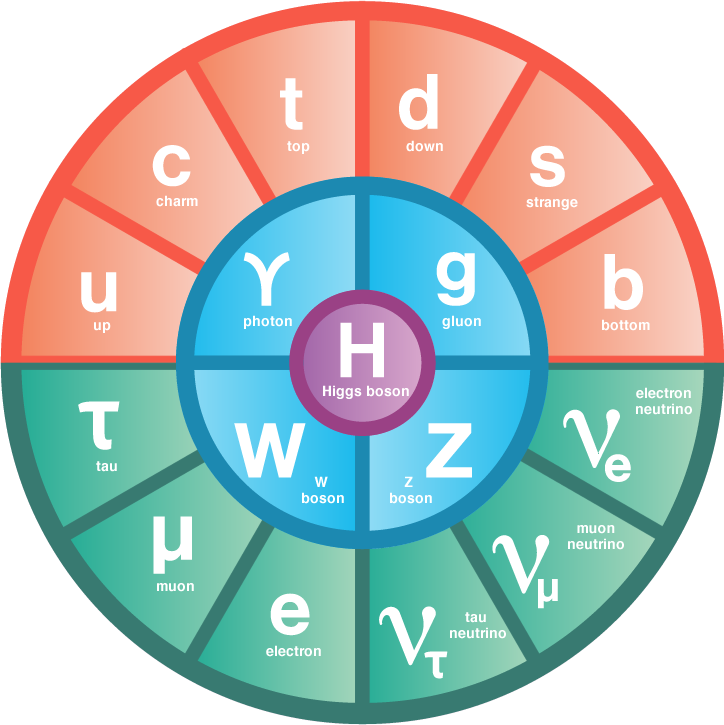
\includegraphics[width=0.45\linewidth]{figures/theory/SM}
\caption{Fundamental particles within the Standard Model}
\label{fig:theory-sm}
\end{center}
\end{figure}

\subsection{Standard Model in QFT Form}

Quantum Field Theory (QFT) the marriage between Quantum Mechanics and Special Relativity, is the modern formalism to describe fundamental physics. In the language of QFT, fields of creation and annihilation operators allow us to calculate the probability distributions of particles which are excited states of fields over time and space. The Standard Model is a special gauge QFT which is invariant with respect to the internal (gauge) $SU(3)\times SU(2)\times U(1)$ symmetry. The gauge symmetries, which give birth to the gauge bosons, are field local symmetries in addition to the global symmetries such as spatial and time. 

The Lagrangian which governs the motion of SM particles can be separated into two parts: $SU(3)$ and $SU(2)\times U(1)$. The $SU(3)$ part of the Lagrangian corresponding to the strong interaction goes as in Eq.\ref{eq:l-su3}. The first term has $F^{a}_{\mu\nu}  = \partial_{\mu}G^a_{\nu}-\partial_{\nu}G^a_{\mu}+g_3f^{abc}G^b_{\mu}G^c_{\nu}$, where $G$ is the gauge field (in this case gluons), $f^{abc}$ is the structure constant of $SU(3)$ group and $g_3$ is the coupling strength for strong interaction. The second term has $\slashed{D} = \gamma^{\mu}(\partial_{\mu}- i\frac{g_3}{2}\lambda^aG^a_{\mu})$, where $\gamma$'s are the Dirac matrices, the $\lambda$'s are the $SU(3)$ matrices and $\psi$ are the quark fields. 
\begin{equation}
  \mathcal{L}_{SU(3)} = -\frac{1}{4}F^{a}_{\mu\nu}F_{a}^{\mu\nu}+ \bar{\psi}(i\slashed{D}) \psi
  \label{eq:l-su3}
\end{equation}

The $SU(2)\times U(1)$ part of the Lagrangian is the unified theory which combines electromagnetic and weak forces. Both kinds of forces exhibit similar properties in the energy scale of \GeV and can be regarded as the same kind of force. This part of the Lagrangian has the same terms as in Eq.\ref{eq:l-su3}, replacing the gauge/fermion fields, structure constants, coupling strength and group matrices to be the corresponding ones in $SU(2)$ and $U(1)$. Note that $U(1)$ group is Abelian and hence $f^{abc}=0$ and the group matrix is a number, while for $SU(2)$ the group matrices are the Pauli matrices ($\sigma$). 


\section{Higgs Physics}
\label{sec:theory-higgs}
\subsection{The Broken Symmetry}

Quarks, charged leptons and weak interaction gauge bosons have mass. From the previous section, the Lagrangian at this point does not explicitly provide mass to these particles. The mechanism through which these particles acquire mass is called spontaneous symmetry breaking.

Recall that the Higgs potential is of the from $V(\phi)=(\frac{1}{2}\mu^2\phi^{\dagger}\phi+\lambda(\phi^{\dagger}\phi )^2)$. Let us denote the two components as $\phi^+ = \frac{\phi_1+i\phi_2}{\sqrt{2}}$ and $\phi^0 = \frac{\phi_3+i\phi_4}{\sqrt{2}}$. If the term $\mu^2<0$, then the potential follow a Mexican hat shape in the 2-dimensional space as shown in Fig.\ref{fig:theory-mexican} and has a minimum at $\phi^{\dagger}\phi = \frac{-\mu^2}{2\lambda} = \frac{\nu^2}{2}$, i.e. the Higgs field acquires a vaccum expectation value. Let us now expand the theory among the direction where $\phi_0 = \frac{1}{\sqrt{2}}\begin{psmallmatrix*}[r]0\\ \nu+H \end{psmallmatrix*}$, i.e. $\phi_3=\nu+H$ and  $\phi_1=\phi_2=\phi_4 = 0$. Once we have chosen a specific direction, the $SU(2)\times U(1)$ symmetry is broken.


\begin{figure}[htpb!]
\begin{center}
  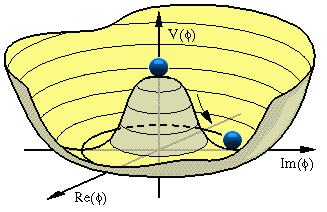
\includegraphics[width=0.45\linewidth]{figures/theory/MexicanHat.png}
\caption{Mexican Hat Potential}
\label{fig:theory-mexican}
\end{center}
\end{figure}


Now, recall from Eq.\ref{eq:l-su21}, since $D_{\mu}$ takes the form in Eq.\ref{eq:SU2U1D}, the covariate derivatie of $\phi$ conatains a term as shown in Eq.\ref{eq:SU2U1cov}, where three degree of freedoms of the original $SU2$ and $U1$ gauge bosons now have mess terms and transform to physical massive $W^{\pm}$ and $Z$ bosons, and one degree of freedom remains massless as the physical photon $\gamma$. 

\begin{equation}
 D_{\mu}  = \partial_{\mu}-ig_1\frac{Y}{2}B_{\mu} - ig_2\frac{\sigma}{2}W_{\mu}
  \label{eq:SU2U1D}
\end{equation}


\begin{equation}
  \begin{split}
   &\phi^{\dagger}(ig_1\frac{Y}{2}B_{\mu}+ig_2\frac{\sigma}{2}W_{\mu})^{\dagger} (ig_1\frac{Y}{2}B_{\mu}+ig_2\frac{\sigma}{2}W_{\mu}) \phi  \\
   =& (\frac{1}{2}\nu g_2)^2 W_{\mu}^+W^{-\mu} + \frac{1}{2}(\frac{1}{2}\nu \sqrt{g_1^2+g_2^2})^2 Z_{\mu}Z^{\mu} + \text{H field terms, where}\\
   &W^{\pm} = \frac{1}{\sqrt{2}}(W^1\mp iW^2) \text{, } Z = -\sin{\theta_W}B+\cos{\theta_W}W^3 \text{ and } \cos{\theta_W} = \frac{g_2}{\sqrt{g^2_1+g^2_2}}
  \end{split}
  \label{eq:SU2U1cov}
\end{equation}


Similarly, the Yukawa couplings in Eq.\ref{eq:l-su21} after symmetry breaking gives mass to the fermions. The expanded terms for electron, for example, is $\mathcal{L} = m_e\bar{e} e + \frac{m_{e}}{\nu}\bar{e}e H$. Two aspects of lepton mass are worth commenting. First, there are no right handed neutrinos, hence the neutrinos do not interact with the Higgs boson. Secondly the coupling of lepton fields with higgs has a strength which is proportional to the mass of the lepton. Hence the heavier the lepton fields are, the stronger the interaction is. For quarks, one more complication arises. The Yukawa coupling is not diagonal. Generations of quarks can mix through the unitary complex CKM matrix.

Finally the Higgs boson gets its own mass through self-interaction term in the Higgs potentail after symmetry breaking. The free parameters of the Standard Model has thus been all revealed to us. There are 9 mass parameters for the fermions and 4 parameters for the quark CMK matrix. Each gauge symmetry gets one free coupling parameter while the strong interaction has one more parameter called QCD vaccum angle. On the Higgs side, the vaccum expectation and Higgs mass are free parameters. In total, the theory has 19 free parameters. All parameters, with the Higgs mass measured by Run I ATLAS and CMS experiments measured to be roughly 125\GeV[ref needed], have been revealed. 


\subsection{Higgs Phenomenology}

The Standard Model Lagrangian dictates the possible Higgs couplings. On the decay side, the Higgs branching ratio is shown in Fig. \ref{fig:theory-higgsbr}. At $M_H = 125\GeV$, the most probable decay mode of Higgs is \Hbb. Recall that the Higgs to fermion coupling strength is proportional to the fermion mass. Although the top quark is way heavier than the bottom quark, the Higgs is not heavy enough to produce on-shell top pairs. On the production side, the Higgs production cross sections of different modes are shown in Fig. \ref{fig:theory-higgsp}. The Feymann diagrams of the leading four production modes: (1) gluon fusion (2) vector bosn fusion (3) associated production and (4) $t\bar{t} H$ production are shown in Fig. \ref{fig:theory-higgsfeymann}


\begin{figure}[htpb!]
\begin{center}
  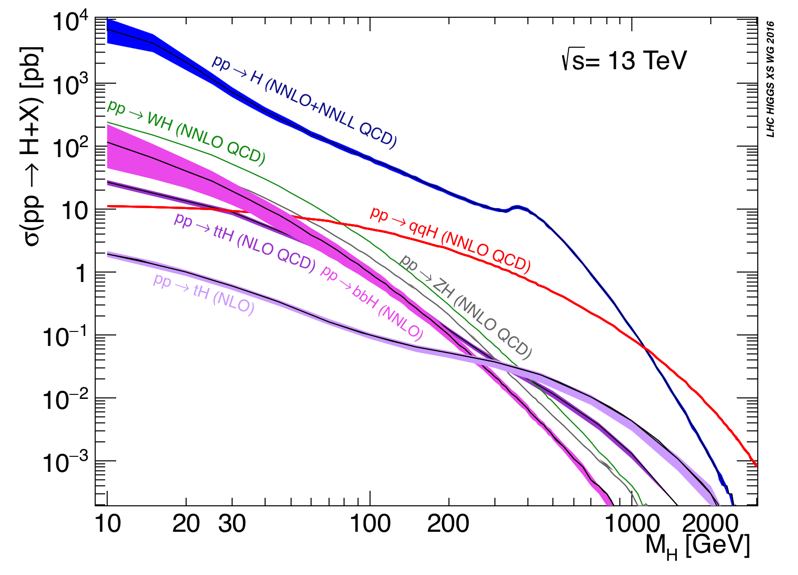
\includegraphics[width=0.6\linewidth]{figures/theory/HiggsCrossSection.png}
\caption{Higgs Production Cross Section at $\sqrt{s}= 13\tev$}
\label{fig:theory-higgsp}
\end{center}
\end{figure}

\begin{figure}[htpb!]
\begin{center}
  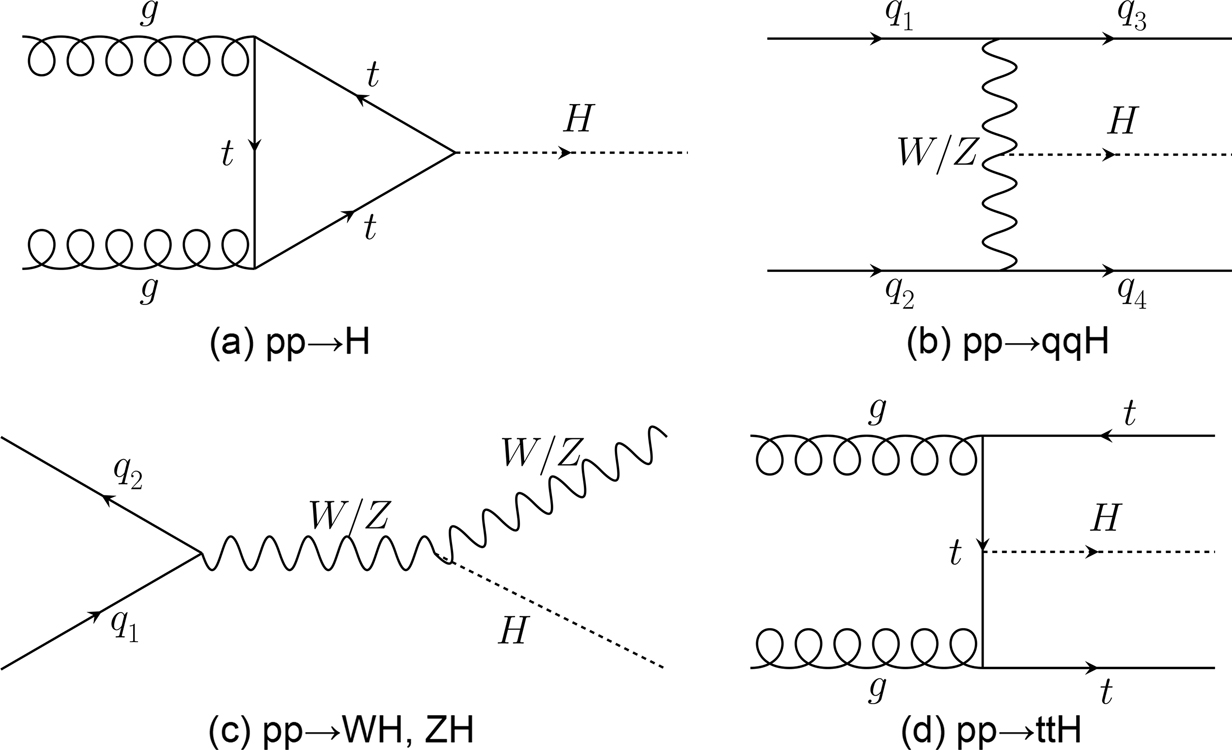
\includegraphics[width=0.45\linewidth]{figures/theory/ProductionFeymann}
\caption{Leading Higgs production Feymann Diagrams ranked in order of strength from (a) to (d)}
\label{fig:theory-higgsfeymann}
\end{center}
\end{figure}


To establish a discovery, particle physics community has agreed on that the observation of the signal significance roughly goes as $\frac{S}{\sqrt{B}}$ have to be greater than $5\sigma$. That is saying, in our measurements, the background-only model has less than $5.8\times 10^{-7}$ chance to fluctuate and generate the data we are seeing. Therefore, the sensitivity of Higgs search should not only consider the cross section of a specific channel which is the product of Higgs production cross section times and branching ratio, but also take into account the irreducible backgrounds. The discovery of Higgs in 2012 was not made through gluon fusion with Higgs decaying to bottom quarks, which has the largest cross section, but through three channels \Hgammagamma, $h\rightarrow ZZ^{(*)}$ and $h\rightarrow WW^{(*)}\rightarrow l\nu l\nu$\cite{HIGG-2012-27,CMS-HIG-12-028}, as the Standard Model di-photon and di-boson processes are orders of magnitude weaker than fully hadronic final state QCD processes. The combination of Run I 7 and 8 \tev data also found evidence of the Higgs Yukawa coupling to $\tau$ with greater than $3\sigma$ significance through the combination of its $\tau_{\text{lep}}\tau_{\text{lep}},\tau_{\text{lep}}\tau_{\text{had}}$ and $\tau_{\text{had}}\tau_{\text{had}}$ decays \cite{HIGG-2013-32,CMS-HIG-13-004}. Meanwhile, the Run I searches of \Hbb decay were not conclusive. ATLAS and CMS searches measured signal signifiance to be 1.4 and 2.1 (2.6 and 2.1 expected)\cite{HIGG-2013-23,CMS-HIG-13-012}. The Higgs to quark Yukawa coupling still remains to be confirmed. 

\begin{figure}[htpb!]
\begin{center}
  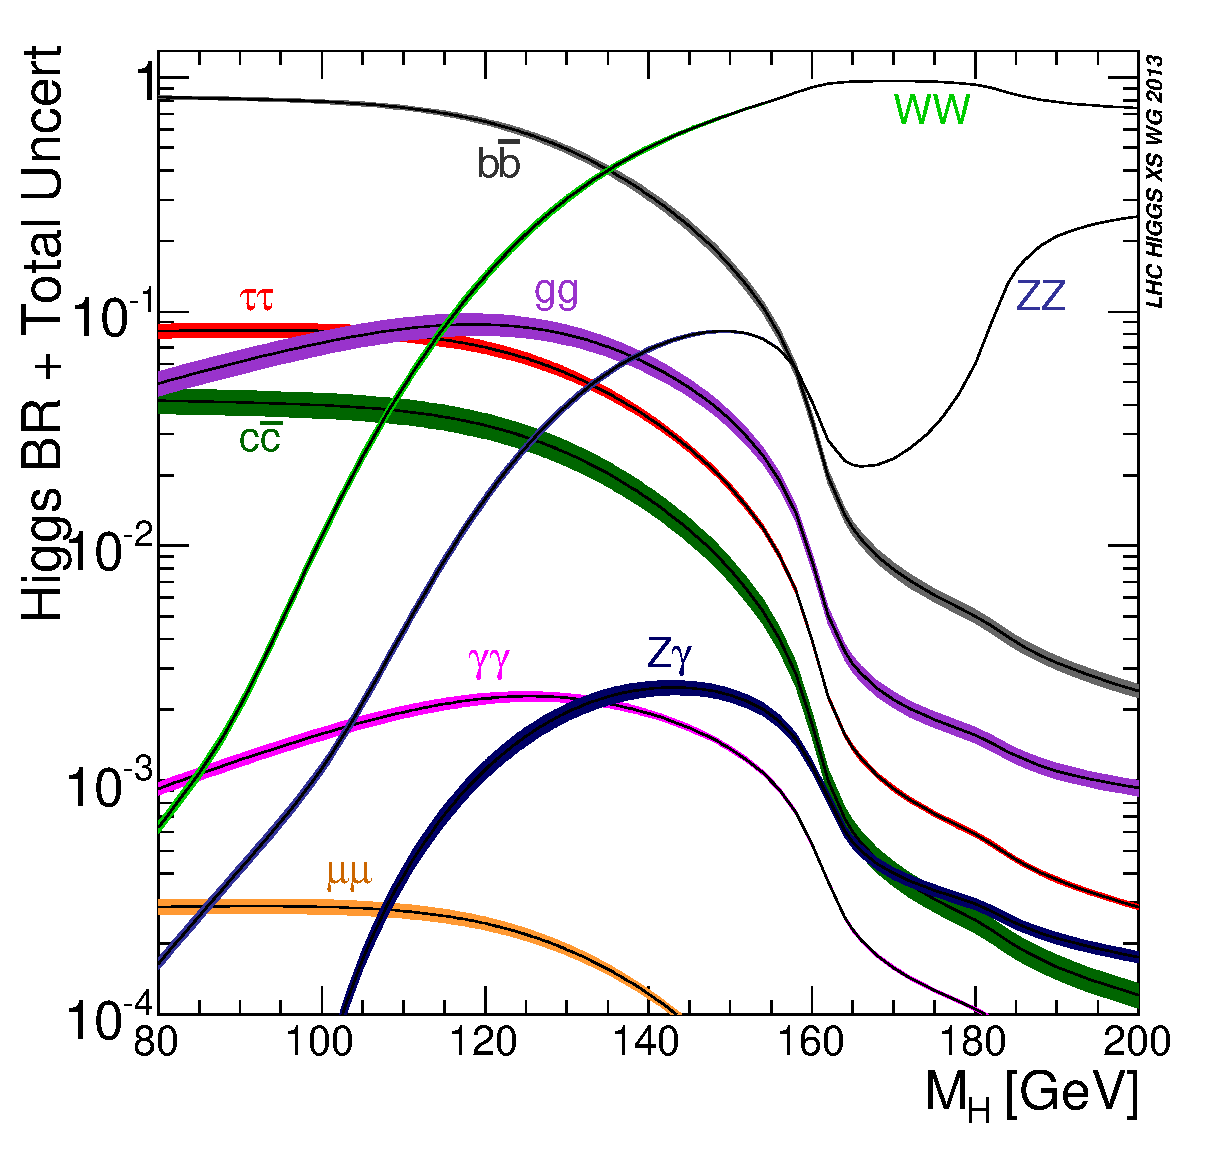
\includegraphics[width=0.45\linewidth]{figures/theory/Higgs_BR_LM.eps}
\caption{Higgs Branching Ratios as a function of hypothetical Higgs mass}
\label{fig:theory-higgsbr}
\end{center}
\end{figure}





\chapter{The Large Hadron Collider}
\label{chap:collider}
\section{The Machine}

In some sense, particle physicists conduct high energy physics experiments in an unimaginative way. To study what is inside the proton we accelerate them to very high speeds and smash them together to see what comes out. The searches of Higgs boson relies heavily on accelerators which have high enough center of mass energy to produce them. The Large Hadron Collider is the largest physics experiment ever constructed in the history of mankind. The designed maximum center of energy can reach 14\tev. The cancellation of the US super-conducting super-collider made the LHC the most powerful accelerator in the world. In a scale of 10 years, the LHC will retain this title for a long time, as no country has expressed explicit interest in constructing the next collider. As the US has terminated the operation of the Tevatron, the LHC is also the only machine with which the Higgs boson can be studied at the moment.

The LHC is located across the border between Switzerland and France. It is one of the accelerators of the accelerator complex at the European Organization for Nuclear Research (CERN) based in Geneva, Switzerland (Fig.\ref{fig:lhc-CERN}). The tunnel of the LHC is 27 km in circumference and 100 meters underground. Before the LHC era, the tunnel was used to host an electron-positron collider called LEP\cite{refneeded}. Two beams of particles go around the accelerator in opposite directions and cross each other at four interaction locations where four experiments, ATLAS, CMS, ALICE and LHCb are located. Proton-proton collisions are the main usage of the LHC, while usually during the last few weeks of operations of each year the machine also collides heavy ions.

\begin{figure}[htpb!]
\begin{center}
  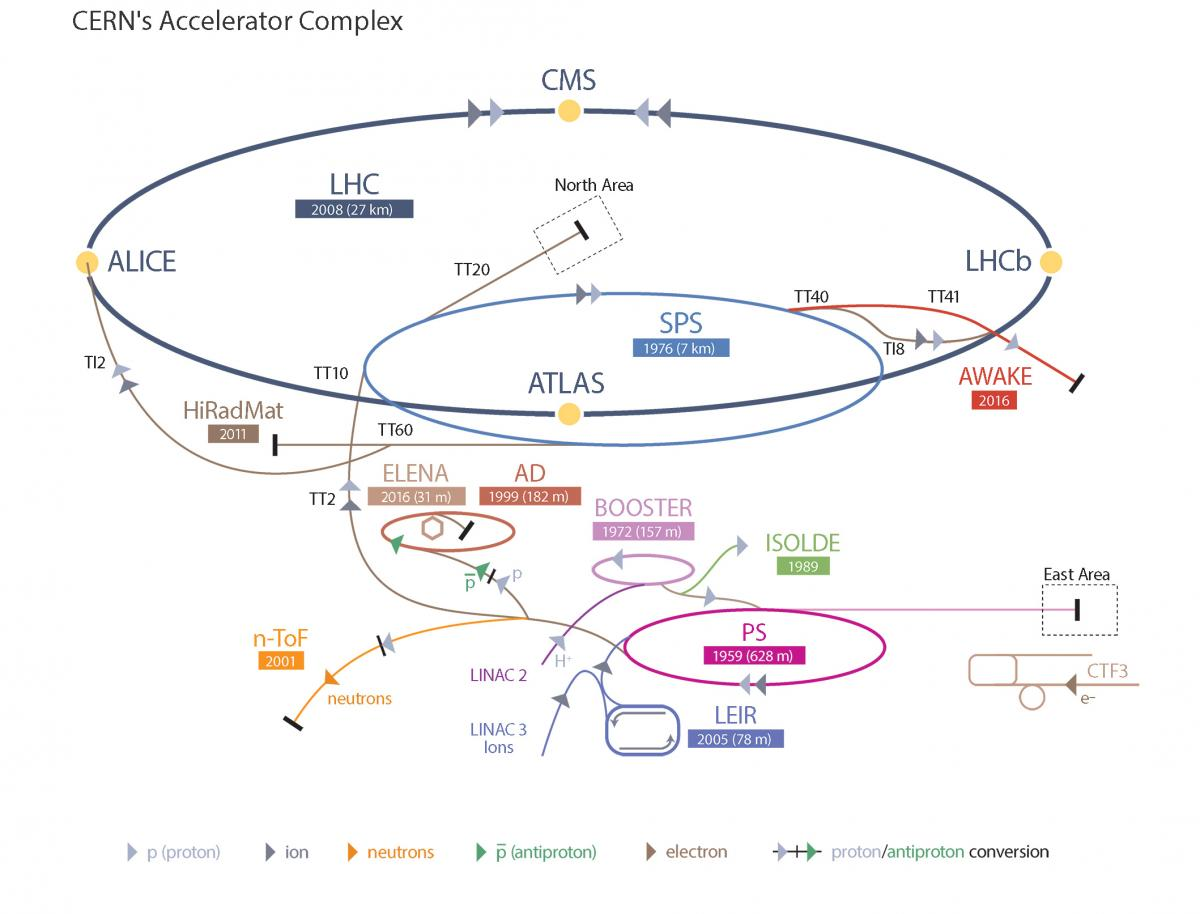
\includegraphics[width=0.7\linewidth]{figures/LHC/LHC_default}
\caption{Diagram of the CERN Accelerator Complex}
\label{fig:lhc-CERN}
\end{center}
\end{figure}


Acceleration of the protons are staged. Many smaller accelerators built for past lower energy experiments are utilized to pre-accelerate the beams before injecting them to the LHC. We obtain the protons from hydrogen gas and first put them through the very first linear acceplerator, the Linac2. The outcoming protons are accelerated to 50\mev and enter a small ring accelerator of radius 25 meters called Proton Synchrotron Booster to be accelerated up to 1.4\gev. Then the protons are fed into the Proton Synchrotron, which is 100 meters in radius, and accelerated to 25\gev. The Super Proton Synchrotron of radius 6.9 kilo-meters then accelerate the beams to 450\gev and eventually inject the beams into the LHC. The LHC depending on its configuration accelerates the beams to 7 to 14\tev.

Radio Frequency (RF) cavities are used by the LHC to accelerate particles. Each of the LHC beam has 8 RF cavities, each of which delivers 2MV acceleration to the particles. The frequency of the RF cavities are held at 400$MHz$ which is an integer multiple (harmonic number $\approx$ 35600)of the revolution frequency $f$ of the proton beam so that the only protons of specific energies are accelerated. To bend the protons inside the circular accelerator, super-conducting magnetic dipoles are used. For the LHC to operate at 13\tev, the dipole field strength needed is about 8.33 telsa. The LHC, employs in total 1232 dipoles which are built with NbTi coils which needed to be cooled down to 1.9$K$ with superfluid Helium to reach super-conductivity.

Most of the collisions at the LHC are generic QCD events, and we are able to produce interesting particles such as Higgs only with very small probabilities (see Fig.\ref{fig:lhc-lhccrossection}). Therefore, we need to collide as many pairs of protons as possible to accumulate sufficient statistics. The beams at the LHC contain proton bunches which are spaced at 25ns. The nominal proton beams in LHC come with 2808 bunches with each bunch containing $1.15\times 10^{11}$ protons in a beam size of 3.5 micrometers. Since 2016, the filling scheme of the LHC changed to Batch Compression Merging and Splitting (BCMS \cite{BCMS}) and reduced the number of bunches down to 2556 per ring while also reducing the beam size down to 2.5 micrometers and retaining $1.15\times 10^{11}$ protons per bunch. As the LHC delivers round symmetric beams, this change yielded brighter beams by lowering the bunch emittance in the instantaneous luminosity equation \ref{eq:lumi}. In Eq.\ref{eq:lumi}, N is the number of protons per bunch, $n_c$ is the number of crossing bunches, f is the beam revolution frequency, $\gamma$ is the relativistic factor, $\epsilon_n$ is the normalized emittance, $\beta_{\text{ip}}$ is the beta function value at the interaction point and the F factor corrects for luminosity loss due to cross angle. The average number of interactions per bunch crossing at the Interaction Point 1 for the ATLAS experiment from 2015 to 2018 was measured to be $<\mu>=34.2$ shown in Fig.\ref{fig:lhc-mu}. 


\begin{equation}
L = \frac{FN^2 n_c f\gamma}{4\pi \epsilon_n \beta_{\text{ip}}}
\label{eq:lumi}
\end{equation}


\begin{figure}[htpb!]
\begin{center}
  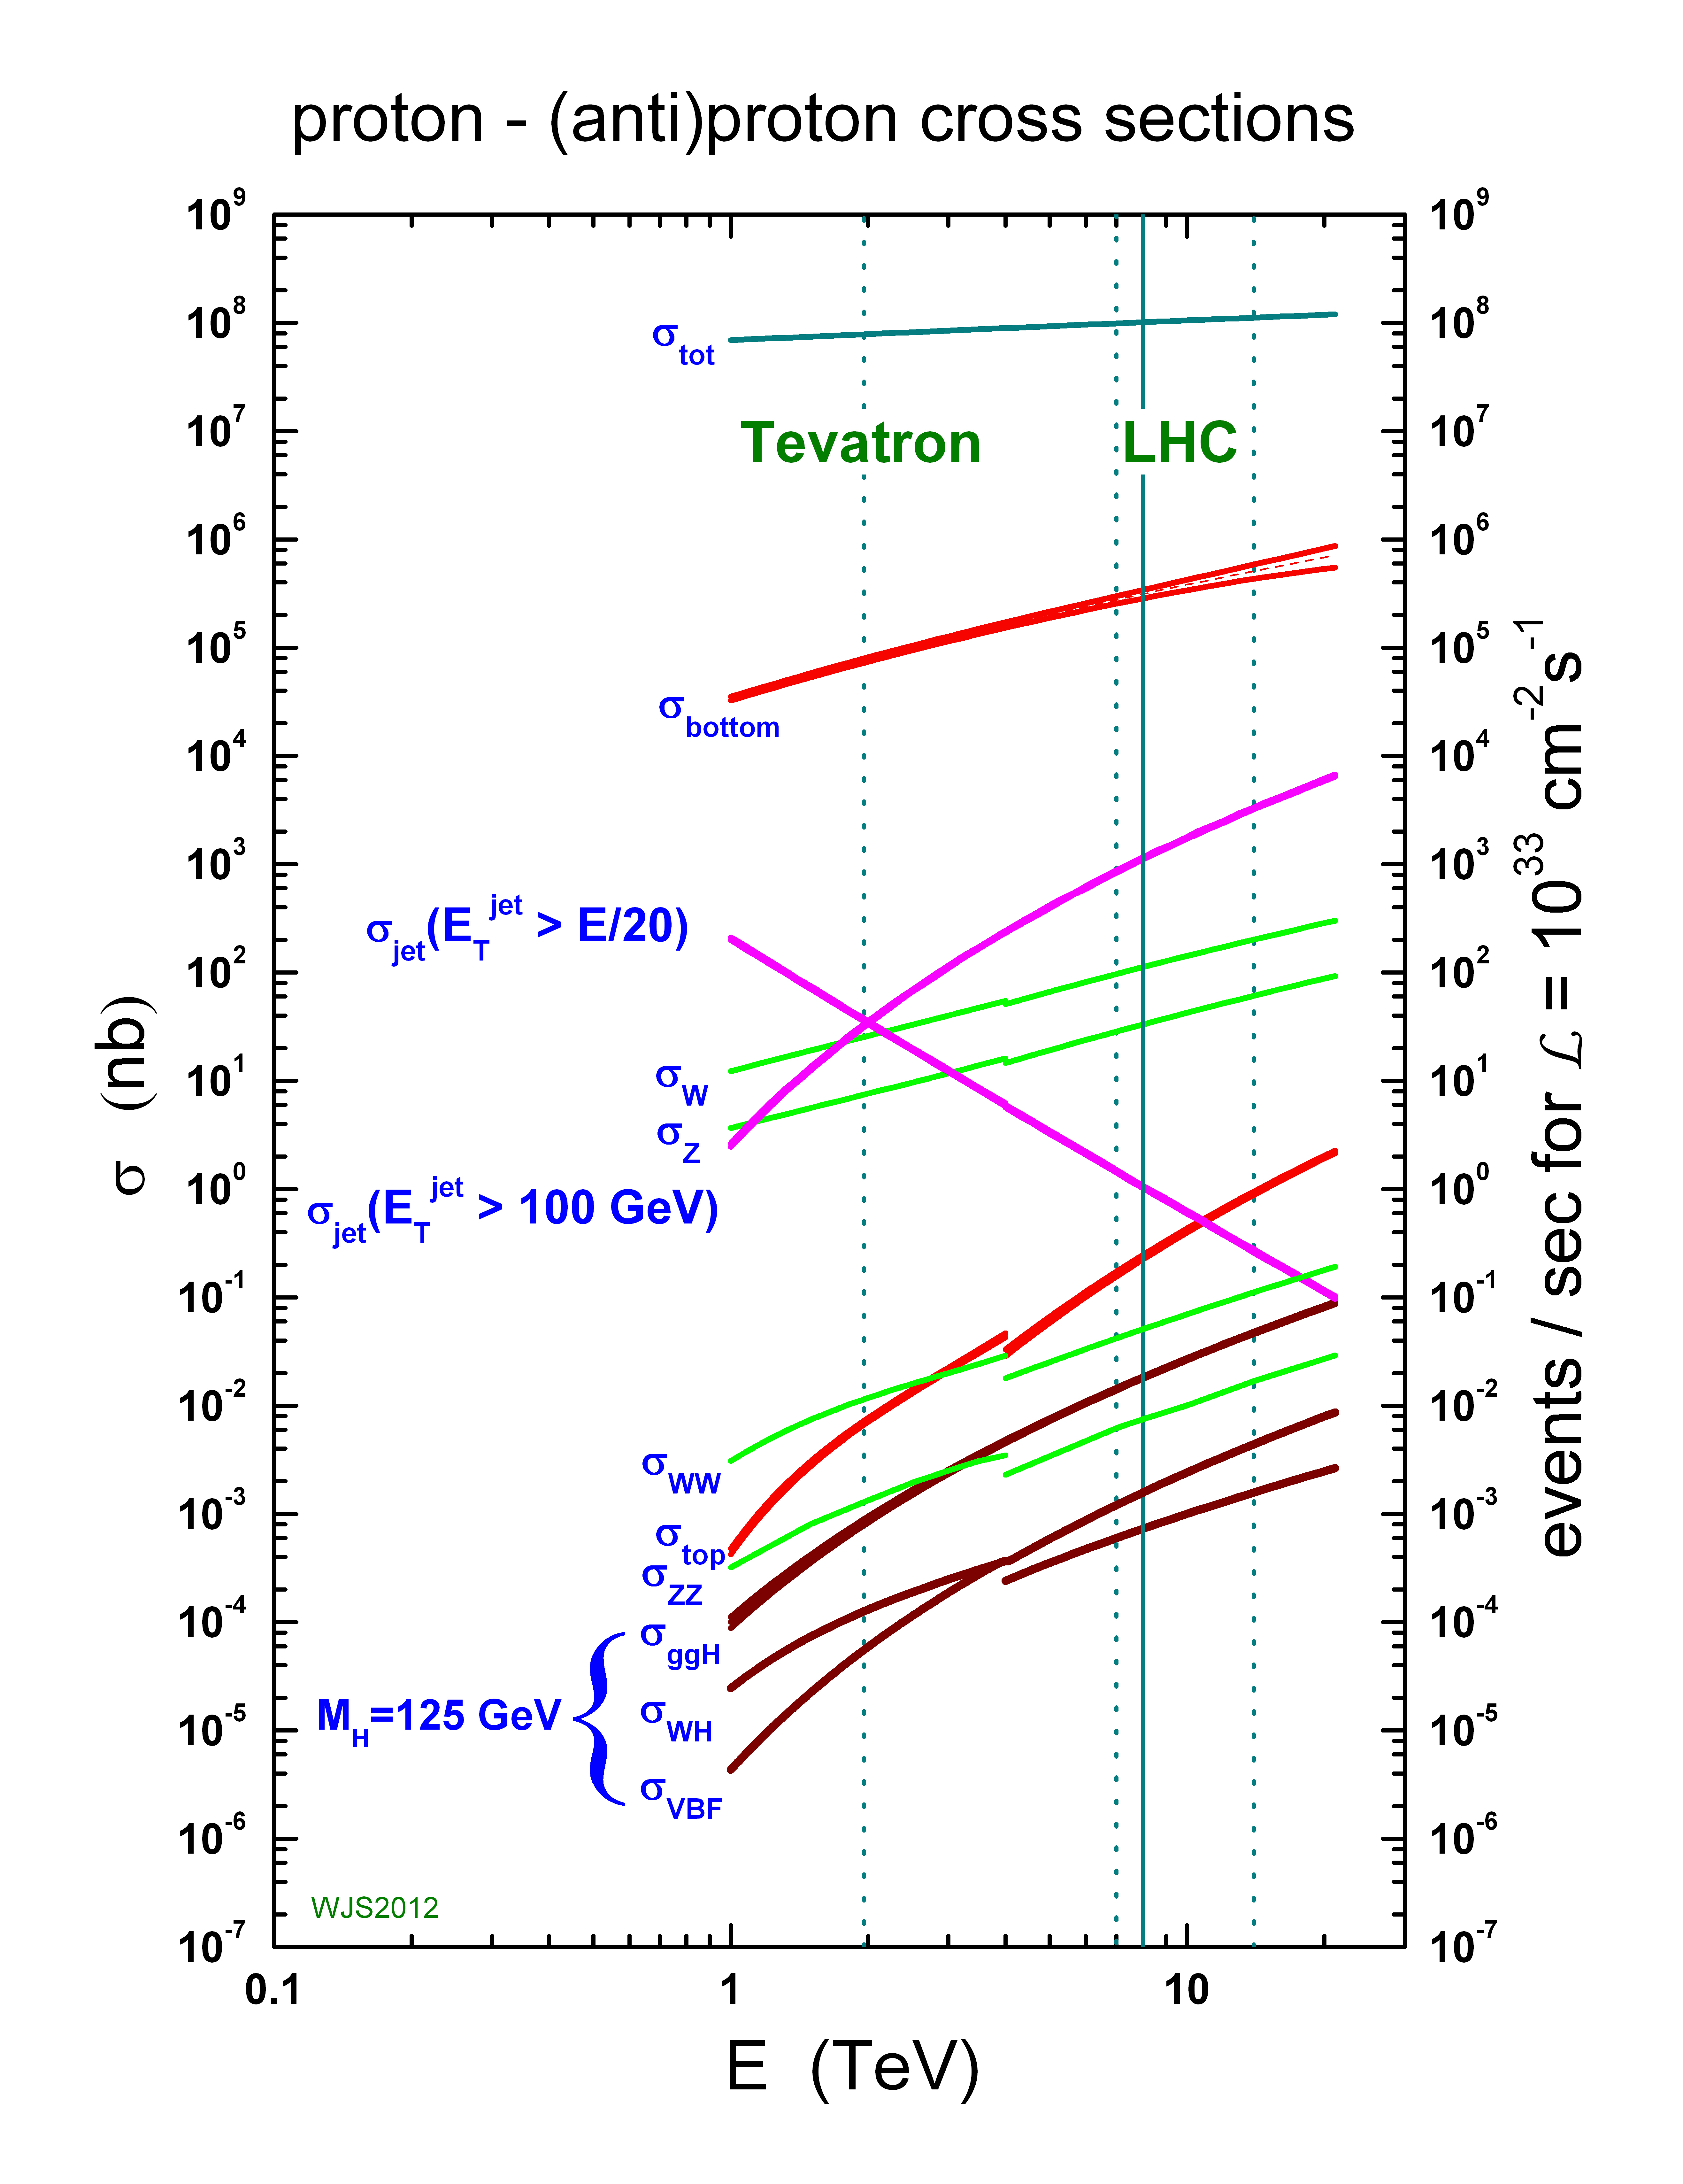
\includegraphics[width=0.6\linewidth]{figures/LHC/crosssections2013}
\caption{LHC Production Cross Sections \cite{stirlingprivate}}
\label{fig:lhc-lhccrossection}
\end{center}
\end{figure}

\begin{figure}[htpb!]
\begin{center}
  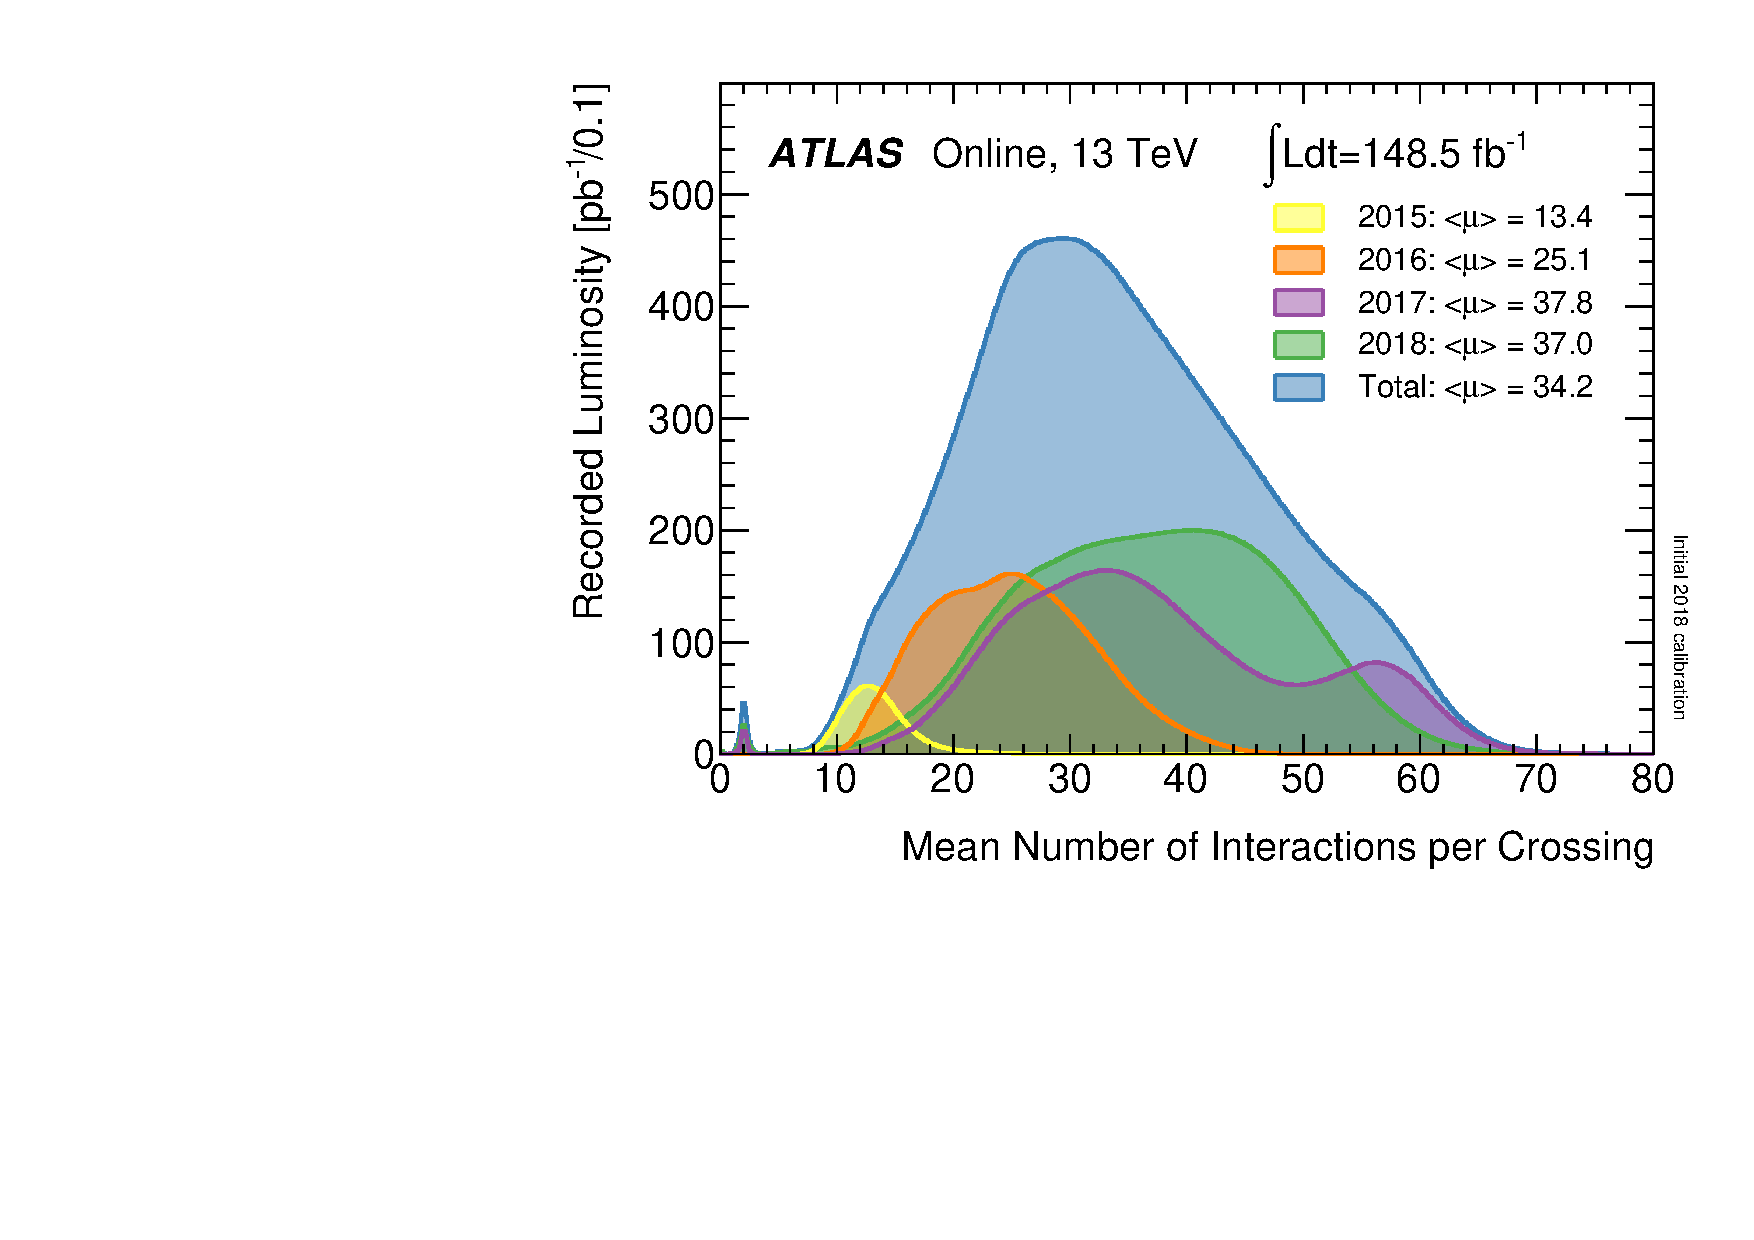
\includegraphics[width=0.6\linewidth]{figures/LHC/mu_2015_2018}
\caption{Number of interactions per bunch crossing at the ATLAS detector}
\label{fig:lhc-mu}
\end{center}
\end{figure}

\section{Operations}

The LHC operations are interleaved between Runs and Long Shutdowns. The Run I experiments start in 2011. The energy of the collider rampped up from 7 to 8\tev and deliver in total 30 \ifb. After the Long Shutdown from 2013 to 2014 (LS1), the machine restarted in 2015 with energy of 13\tev for Run II operation to deliver 150 \ifb of data. The machine now is in the second Long Shutdown (LS2) and will restart in 2021 for Run III operation with 14\tev to deliver 300 \ifb of data. Eventually, after experiments upgrade, the LHC will enter HL-LHC era and keep running to deliver 3000\ifb of data. This thesis primarily uses the datasets collected during Run II LHC operation by the ATLAS detector. The luminosity accumulation through this period is shown in Fig.\ref{fig:lhc-lumi}. Specifically, analyses in this thesis used the 2016 dataset which amounts to 36 \ifb.


\begin{figure}[htpb!]
\begin{center}
  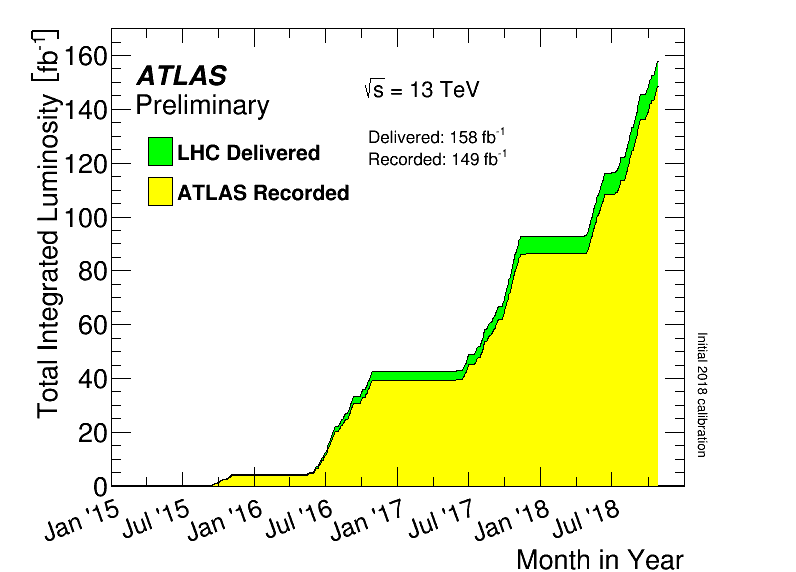
\includegraphics[width=0.6\linewidth]{figures/LHC/intlumivstimeRun2.png}
\caption{Integrated luminosity delivered by the LHC and collected by the ATLAS detector during the Run II experiment. The 2015 run was mostly a trial to test the collider and detector conditions after the LS1.}
\label{fig:lhc-lumi}
\end{center}
\end{figure}

\clearpage

\chapter{ATLAS Detector}
\label{chap:detector}
The name ATLAS is short for \textit{A Toroidal LHC Apparatus}. It is a multi-purpose particle detector which is designed primarily to detect and measure particles coming out of proton-proton collisions. The detector is located 100 meters underground at the LHC point one so that it is shielded from cosmic rays and weighs about 7000 tons. The ATLAS detector has a forward-backward symmetric cylindrical geometry with radius of 25 meters and length 44 meters. Over three thousand collaborators work at the ATLAS experiment. By design and for cross validation purpose, the ATLAS detector is very similar in regard of its functionality to its counterpart the CMS (Compact Muon Solenoid) detector at LHC point five. 

The collaboration uses a right-handed coordinate system as the convention. The beam pipe which penetrates through the detector is the $z$-axis of the coordinate system, while the origin of which is the beam interaction point (IP) also the center of the detector. The $x$-axis points from the origin of the detector towards the LHC ring center while $y$ axis points upward to the ground. Cylindrical coordinate is used in addition to the Cartesian coordinate described above. The $x-y$ plane parameterized by ($r,\phi$) where $r$ is the radius inside the plane and $\phi$ is the azimuthal angle around the beam. A polar angle $\theta$ is also defined with respect to the beam. The particle pseudorapidity defined as $\eta = -\ln \tan(\theta/2)$ is more commonly used than the polar angle as the difference between two massless particles' pseudorapidity is Lorentz invariant. The measure in the angular plane is defined as $\Delta R = \sqrt{\Delta \phi^2+\Delta \eta^2}$.

The ATLAS detector has approximately $4\pi$ coverage in solid angle. It contains many sub-systems as shown in Fig.\ref{fig:detector-atlas} which are used to measure different properties of the particles as well as distinguish different types of them. The major sub-components are the inner tracking detector, electromagnetic and hadronic calorimeters, and a muon spectrometer. There is also a dedicated data acquisition system to read out, filter and save the massive amount of data collected by these systems. The inner-most part of the detector is the inner detector,more details to be found in Sec.\ref{sec:detector-id}, primarily used to measure the charged-particle trajectories. A superconducting solenoid provides 2T magnetic field pointing in the $z$ direction can bend the charged-particles which will leave energy deposits on the layers of the inner detector, first few of which are silicon pixel layers followed by semiconductor microstrips (SCT) and then a transition radiation tracker (TRT). Most of the particles produced from the collisions end their journey in the calorimeter system, see Sec.\ref{sec:detector-calo}. The combination of electromagnetic lead/liquid-argon (LAr) calorimeter and the hadronic calorimeter built with steel/scintillator tiles measures the energies of particles. Only neutrinos and muons typically go beyond the calorimeters. Neutrinos hardly interact with materials and escape the detector while muons then enters the muon spectrometer with superconducting toroids providing 4T magentic field as will be described in Sec.\ref{sec:detector-mu}. The data coming out of the detector goes through a trigger system (Sec.\ref{sec:detector-trigger}) in order not to swap the disk. First level of filtering is done with level one trigger (L1) implemented in hardware. Another level of software trigger then accepts events at a even smaller rate. 


\begin{figure}[htpb!]
\begin{center}
  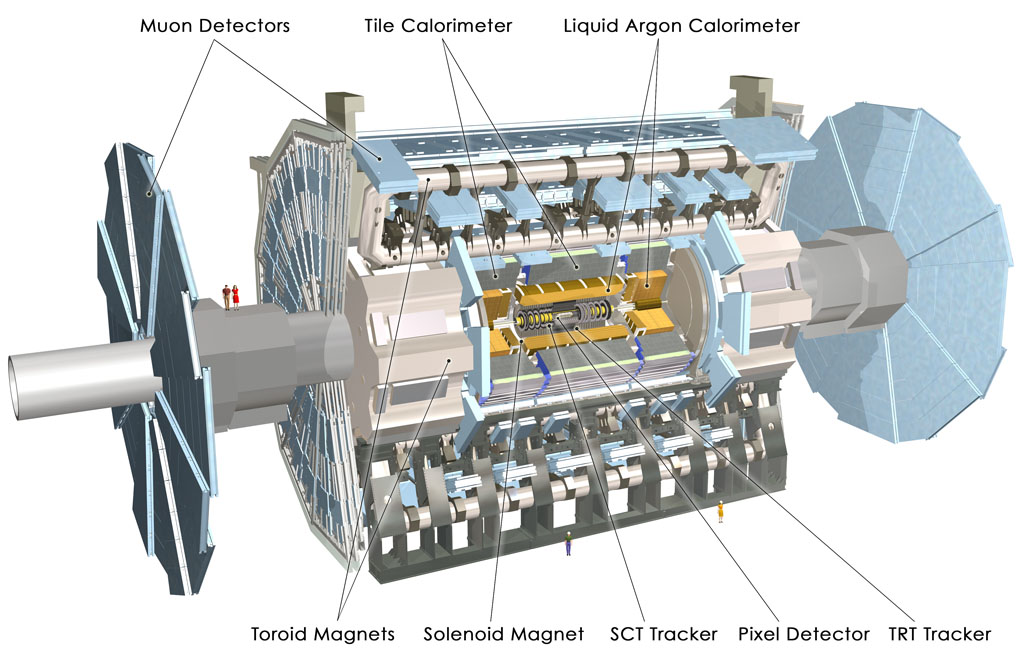
\includegraphics[width=0.85\linewidth]{figures/detector/ATLAS_Silver_White_MK}
\caption{View of the ATLAS detector and its sub-systems}
\label{fig:detector-atlas}
\end{center}
\end{figure}




\section{Inner Detector}
\label{sec:detector-id}

The inner detector (also known as the tracker) consists of three sub-detectors is responsible for vertex finding, charged-particle trajectory finding and momentum measurements. The original design of the inner detector is presented in Fig.\ref{fig:detector-id}, in which it includes three layers of pixel detectors, four double layers of SemiConductor Tracker (SCT) and 36 layers of gaseous straw tubes as transition radiation detector. This design lasted for the entire Run I period for ATLAS. For Run II, the silicon pixel detector was upgraded to include an additional layer inserted at $R=33.25mm$~\cite{CERN-LHCC-2010-013}. The entire tracker covers a pseudorapidity range of $|\eta|<2.5$.


\begin{figure}[htpb!]
\begin{center}
  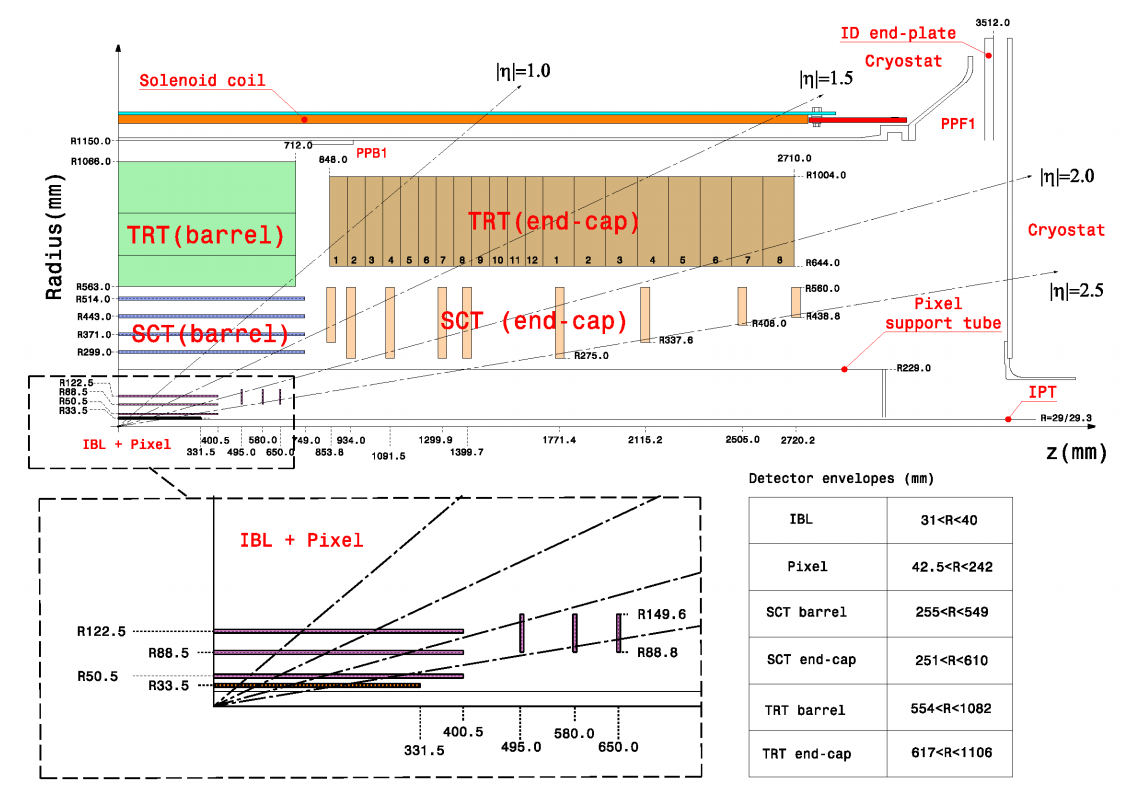
\includegraphics[width=0.9\linewidth]{figures/detector/ID}
\caption{View of a quadrant of the ATLAS inner detector in its original design (not including IBL which is inserted at $R=33.25mm$ for the Run II ATLAS experiment) \cite{SCTpaper}}
\label{fig:detector-id}
\end{center}
\end{figure}



\subsubsection{Pixel}

The pixel detector is the component closest to the beam line to provide best possible spatial resolution. The standard pixel sensors are bonded to readout electronics through the hybridization technique. The Run I ATLAS three pixel layers used the planar design. The size of the pixel is $50\times 400 \mu m^2$, which are limited by the size of the electronics attached to the pixels. For the Run II experiment, the collaboration decided to add another layer of pixel called insertable B-layer (IBL). Since the pixel layers are very close to the beam, radiation damage is a serious concern. The energetic particles such as neutron could knock the silicon atoms out of the lattice leading to higher bias voltage needed to deplete the bulk of the silicon as well as reducing the charge collection efficiency. At the time, a new type of pixel detector design with 3D sensor shown in Fig.\ref{fig:detector-sensor} was available. The 3D sensor collects the charge in the direction perpendicular to that of the planar sensor reducing the drifting path and hence is more radiation hard. However due to a lack of operational experience, the 3D design was only partially adopted (25\% of all the IBL sensors) and used to cover the high $|\eta|$ region (out of the $|\eta|<2.5$ active tracking regime). For the majority of the sensors, the planar design was used with the pixel size reduced to $50\times 250\mu m^2$. 

\begin{figure}[htpb!]
\begin{center}
  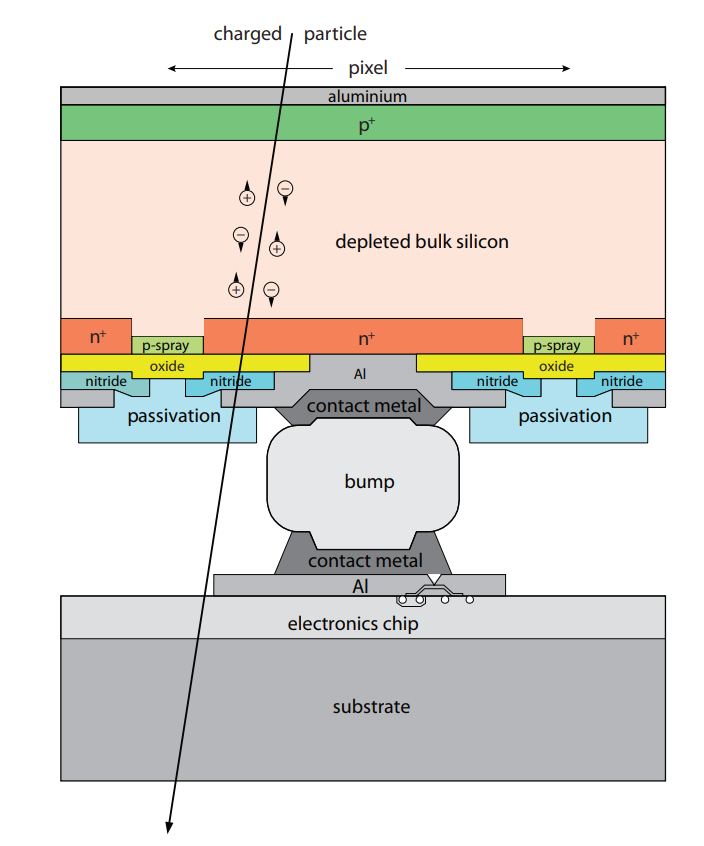
\includegraphics[width=0.35\linewidth]{figures/detector/PixelPlanar}
  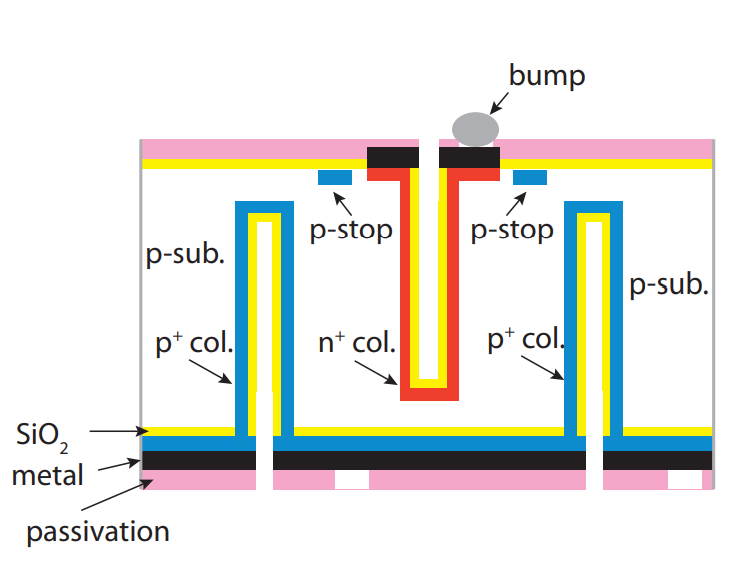
\includegraphics[width=0.40\linewidth]{figures/detector/Pixel3D}
\caption{Examples of planar (left) and 3D (right) pixel designs from \cite{PixReview}. The 3D pixel sensor design has smaller drifting path }
\label{fig:detector-sensor}
\end{center}
\end{figure}


\subsubsection{SCT}

Fabrication and manufacturing of pixel detector are difficult. Before the advent of the pixel detector, microstrips are the first type of silicon trackers. The microstrips instead of reading out the two-dimensional signals directly, places two layers close to each other and reads out one-dimensional signal (hit on a strip) from both layers. The read out electronics hence can be much more simply connected to the sensors. Of course one downside of the design is the large number of ghosts when there are multiple tracks hitting the detector at the same time.

The ATLAS SCT detector adopts the microstrip design. Two sets of sensors of the same layer are rotated 40$mrad$ with respect to each other. The SCT has both the coaxial cylindrical barrel layers and disk-shaped endcap layers. The former of which has 8448 and latter has 6944 sensors\cite{SCTpaper}. Nominal design resolutions are $17\mu m$ in the $R-\phi$ plane and $580 \mu m$ in the $z$-direction \cite{PERF-2007-01}.


\subsubsection{TRT}

The outermost layer of ID is Transition Radiation Detector which serves to both find charged particle hits and identify electrons. The entire TRT consists of 298304 2mm radius straw tubes\cite{TRTpaper} as drift chambers filled with $Xe$, $CO_2$ and $O_2$ during Run I and with $Ar$, $CO_2$ and $O_2$ during Run II to collect the electrons rising from primary ionization of charged particles. In addition, polypropylene fibers with diameter of $19\mu m$ serve as the radiators. Photons emitted primarily from the transition radiations of electrons going across media of different refraction index are signals of electron identification.


\section{Calorimeter}
\label{sec:detector-calo}

The ATLAS calorimeter shown in Fig.\ref{fig:detector-calo} has two major functional components which are the electromagnetic (EM) and hadronic calorimeter which separately measure the EM and hadronic showers shapes of incoming particles and their total energy. Both the EM and hadronic calorimeters at ATLAS are sampling calorimeters. In contrast to homogeneous calorimeters, the absorbers of sampling calorimeters are interleaved with detector components only measure partial energy deposits. Sampling calorimeters are an economic design. Having two sampling calorimeters, ATLAS detector achieve pretty balanced performance between EM and hadrnoic calorimeters while the CMS experiment chose to have an expensive EM calorimeter built of crystals sacrificing the performance of hadronic calorimeter. 


\begin{figure}[htpb!]
\begin{center}
  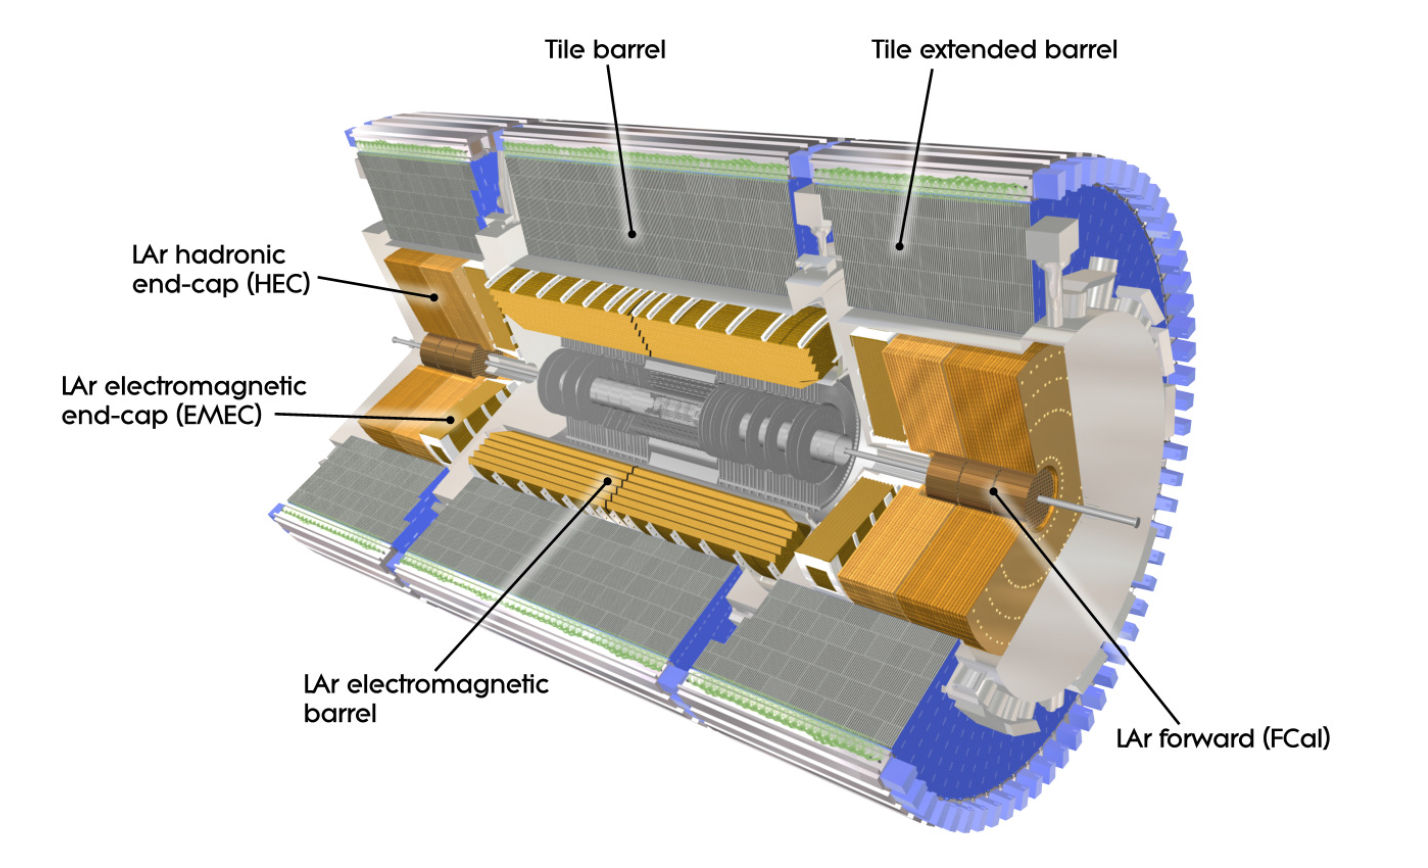
\includegraphics[width=0.9\linewidth]{figures/detector/calo}
\caption{View of ATLAS calorimeter system \cite{LARReadout}}
\label{fig:detector-calo}
\end{center}
\end{figure}

 
\subsubsection{EM Calorimeter}

The lead/liquid-argon EM calorimeter has three components\cite{ATLASDetector}, one with exact $\phi$ symmetry covering the barrel part of the detector and two placed at each endcap covering $|\eta|<3.2$. The barrel part of the EM calorimeter is designed to provide great spatial resolution and is separated into three layers with interaction lengths varying from $22X_0$ to $33X_0$. At $\eta =0$, for instance, the first layer has extremely fine segmentation in $\eta$, i.e $\Delta \eta = 0.0031$ and is able to distinguish different particle types. The second layer is composed of near squares with angular segmentation of $\Delta \eta \times \Delta \phi = 0.025 \times 0.0245$ and has the largest interaction length of 17$X_0$. The third layer has the same $\phi$ resolution and half $\eta$ resolution of the second layer. 
The endcap electromagnetic calorimeter (EMEC) also has two different layers, with the first one having finer segmentation. The EM calorimeter completely operates in cryostats to maintain Ar in liquid state.

\subsubsection{Hadronic Calorimeter}

Hadronic calorimeter surrounds the EM calorimeter. The barrel consists of steel/scintillator tiles and has three subsystems: one central and two extended barrels\cite{ATLASDetector}. This part of the hadronic calorimeter covers $|\eta|<1.7$ and has interaction length of 7.4$\lambda$. The hadronic end-cap calorimeter (HEC) consists of cooper/liquid-argon and has coverage $1.5<|\eta|<3.2$\cite{ATLASDetector}. Another calorimeter dedicated to cover high $|\eta|$ region, the forward calorimeter (FCal), is made of copper-tungsten/liquid-argon\cite{ATLASDetector}. It serves both as an EM and a hadronic calorimeter for the forward region. The entire calorimeter system covers up to $|\eta|=4.9$.






\section{Muon Spectrometer}
\label{sec:detector-mu}
Outside the calorimeters sits the muon spectrometer show in Fig.\ref{fig:detector-mu}. Even though the muon spectrometer only serves to measure and detect the muons, it has profound importance for physics. One of the early concerns for ATLAS and CMS experiments are that the detector's capability to handle the high rate from LHC collisions. The ID and calorimeters could potentially be blacked out. Once channel that still allows us to study the Higgs in such circumstance is the Higgs to four muons, the background of which is also low rate and should be able to handle. Hence the muon system is the safety insurance for ATLAS to produce meaningful physics result. The entire muon spectrometer is divided into four parts. The Monitored Drift Tubes (MDT) and Cathode Strip Chambers (CSC) are the precision chambers used for precision muon measurements, while the Resistive Plate Chambers (RPC) and Thin Gap Chambers (TGC) are used for fast muon triggering. Muons entered into the muon spectrometer are bent the second time by the 4T toroid magnetic field. 

\begin{figure}[htpb!]
\begin{center}
  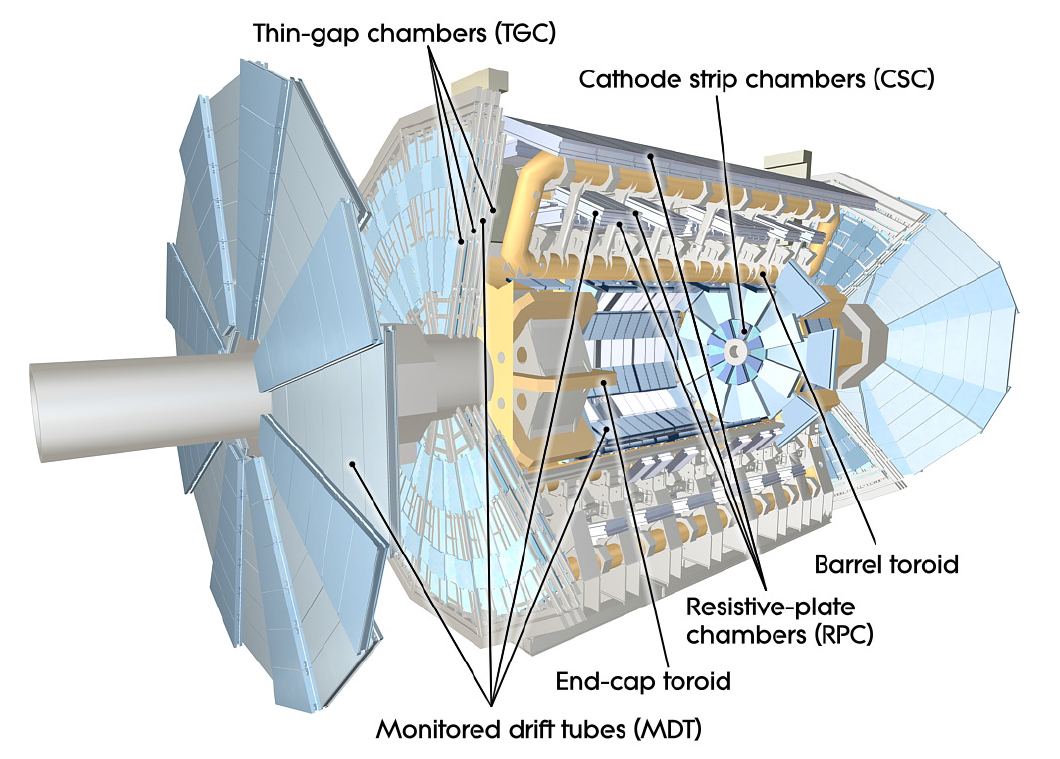
\includegraphics[width=0.8\linewidth]{figures/detector/muon}
\caption{View of ATLAS muon spectrometer}
\label{fig:detector-mu}
\end{center}
\end{figure}


There are three layers of precision chambers at the barrel of the detector and for layers at the endcaps located at the ATLAS large wheels. Most of the layers are MDT which cover $|\eta|<2.7$ except for the innermost layer of the endcap, which uses CSC due to very high rate forward rate. MDT consists of 29.97mm pressurized drift tubes filled with $Ar$ and $CO_2$ gas and provide $35\mu m$ resolution in $z$. Within CSC active gas (also $Ar$ and $CO_2$) volume there are perpendicular cathode strips such that CSC can provide two dimensional coordinate system. The CSC safe operating count rate is 1000 $Hz/cm^2$ much higher than the 150 $Hz/cm^2$ of the MDT with comparable resolution. The RPC modules are made of two resistive plates apply 4.9$kV/mm$ to the gas mixture filled in the short 2$mm$ space in between ($C_2H_2F_4/Iso-C_4H_{10}/SF_6$). They are inserted near the MDT and with reasonable cost can read out safely at 1000 $Hz/cm^2$. The TGC essentially has the same design as CSC but with smaller wire and cathode spacing to allow faster electron drifts. 



\section{Trigger and Data Acquisition}
\label{sec:detector-trigger}


\chapter{Physics Objects Reconstruction and Identification}
\label{chap:reconstruction}
Digital signals from the detectors are processed by software to reconstruct the physics objects in the detector. The most relevant objects for this thesis are the charged particle trajectories (tracks) and bundled decay products of hadrons (jets). This chapter presents the reconstruction methods of them in Sec. \ref{sec:reco-tracking} and \ref{sec:reco-jets} respectively. 


\section{ID Tracks and Vertices}
\label{sec:reco-tracking}
Many algorithms and software designs are available for tracking. For details readers may refer to \cite{Cornelissen:1020106}. The following presents the reader with a brief summary of primary algorithms used by ATLAS as the tracking reconstruction procedure, the so called ``inside-out'' procedure. Track finding starts from the precision detectors pixel and SCT. We first find 3-D representation of pixel and SCT clusters/hits called ``space points''. Then track seed searches are done with three pairs ``space points'' with $z$ constraints (tighter cut on the primary vertices, which are the interaction points of $p\bar p$ collisions) or no constraints (loose cut on primary vertices.) Track seeds at this point contain directional information. The track fitting utilizes Kalman filter assuming the hit sequence to follow Hidden Markov Model. While the filter moves along the track seeds direction, it incorporates the new hits it sees and updates the track fit with five helix parameters at the perigee of the track. Only 10\% of the seeds eventually lead to real tracks. To resolve the ambiguity arising from seeded tracking, track candidates are ranked by their quality scores. Scores favor tracks with high $\chi^2$, less holes and hits from higher resolution part of the detector. Shared hits are then assigned to higher score tracks and lower score tracks are refitted. For very dense environments, in which the pixel clusters may merge, see for example Fig.\ref{fig:reco-trackingcluster}, neural network tools are utilized to separate apart clusters created by no more than two individual charged particles\cite{PERF-2012-05,Aaboud:2017all}. The track segment found by the pixel and SCT collaboratively are then extended to include matched TRT hits. The alignment, which refers to the accurate determination of the tracking detector geometry, of the tracker needs to be performed online to reduce hit to track residuals as the thermal condition of the pixel detector changes during data taking. Especially during the early Run II operation, the IBL was observed to have an unexpected bowing giving rise to an up to 6$\mu m$ vertical shift and needs real time corrections.\cite{tracking-align}.

\begin{figure}[htpb!]
\begin{center}
  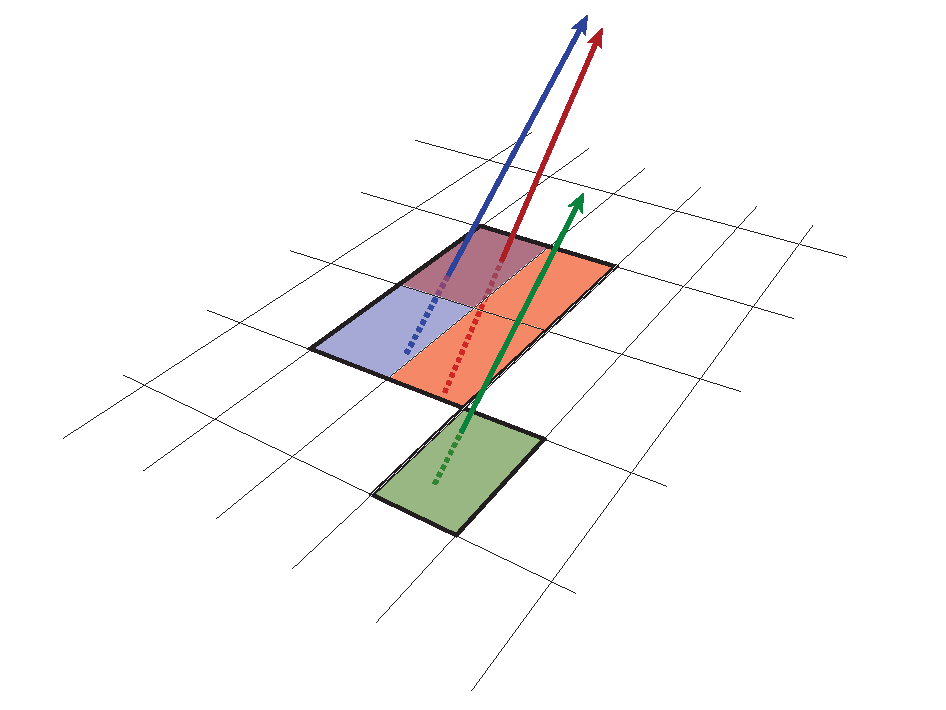
\includegraphics[width=0.55\linewidth]{figures/Reco/TrackingClusterB}
  \caption{ Illustration a merged pixel cluster due to collimated charged particles originating from high energy parent (Ref.\cite{Aaboud:2017all}). }
\label{fig:reco-trackingcluster}
\end{center}
\end{figure}


Tracks used by physics analyses need to pass quality and kinematics cuts. The loose track quality\cite{ATL-PHYS-PUB-2015-018} is defined as:

\begin{itemize}
\item \pT $>$ 400 \mev
\item $|\eta| < $ 2.5
\item At least 7 silicon (pixel + SCT) hits
\item At most 1 shared module, which are modules (1 hit for pixel and 2 hits for the same layer SCT) shared between two reconstructed tracks
\item At most 2 silicon holes, which are charged particle interaction with the tracker materials but left on hits on the tracker 
\item At most 1 pixel holes
\end{itemize}

On top of the criteria of loose tracks, the tight track criteria\cite{ATL-PHYS-PUB-2015-018} include also the following:

\begin{itemize}
\item No pixel holes
\item At least 1 hit on IBL or B-layer
\item Silicon hits $\geq$ 9 (if $|\eta|\leq 1.65$)
\item Silicon hits $\geq$ 11 (if $|\eta|\geq 1.65$)
\end{itemize}

The reconstruction efficiency of tracks depend on the type of decay, initial particle momentum and psuedorapidity and so on. Fig. \ref{fig:reco-trackingeff} shows the per-track tracking efficiency as a function of parent particle \pt in different decay modes. Particularly relevant for this thesis is the efficiency of tracking for $B$ mesons, which with loose track requirement stays reasonably above 85\% up to 1\TeV. When the pile-up contribution goes up, accidental combinations of hits could also pass all the cuts we apply to the track candidates and yield so called ``fake'' tracks. This effect is estimated to be $\leq 5\%$ for the loose category tracks with $\mu = 30$ as shown in Fig.\ref{fig:reco-trackingfake}.


\begin{figure}[htpb!]
\begin{center}
  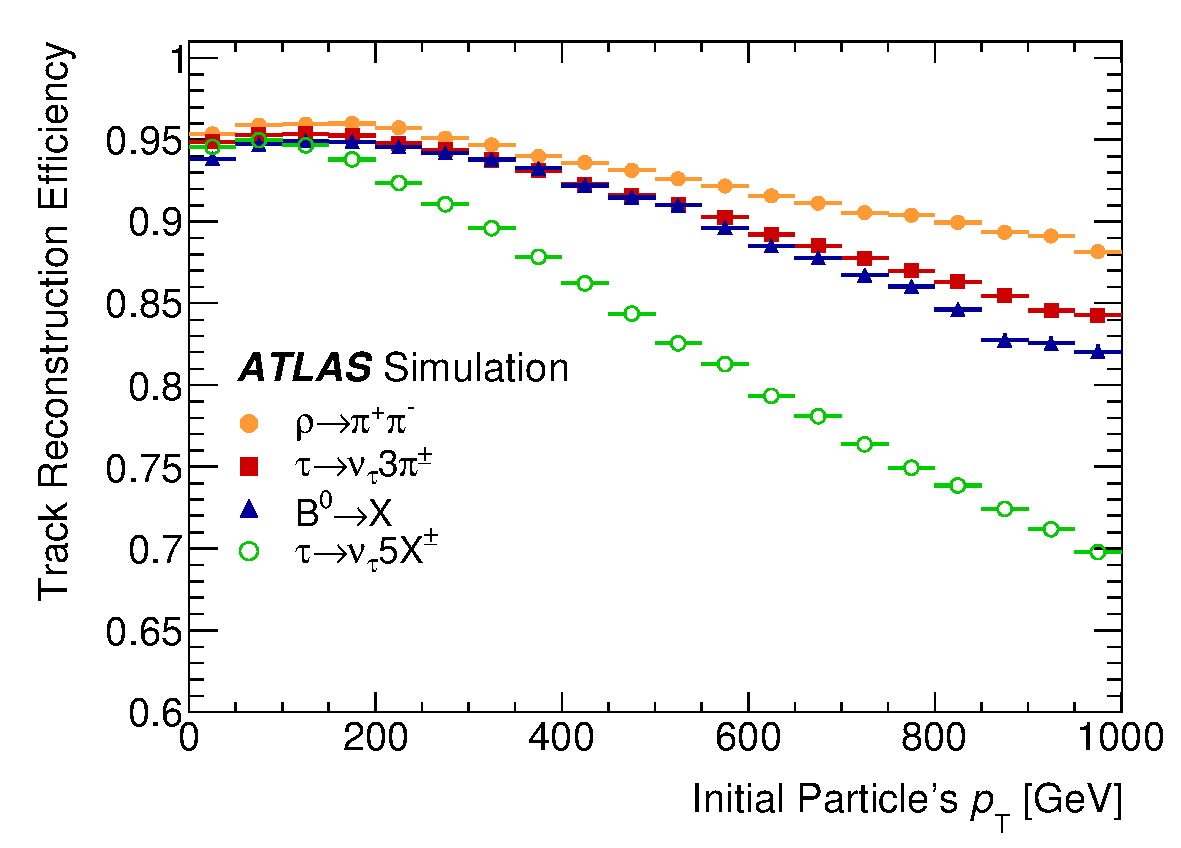
\includegraphics[width=0.55\linewidth]{figures/Reco/TrackingEfficiency}
  \caption{Per-track tracking efficiency as a function of \pt of the parent particle which decays before the IBL for $\rho$, three- and five-prong $\tau$ and B0 (Ref.\cite{Aaboud:2017all})}
\label{fig:reco-trackingeff}
\end{center}
\end{figure}

\begin{figure}[htpb!]
\begin{center}
  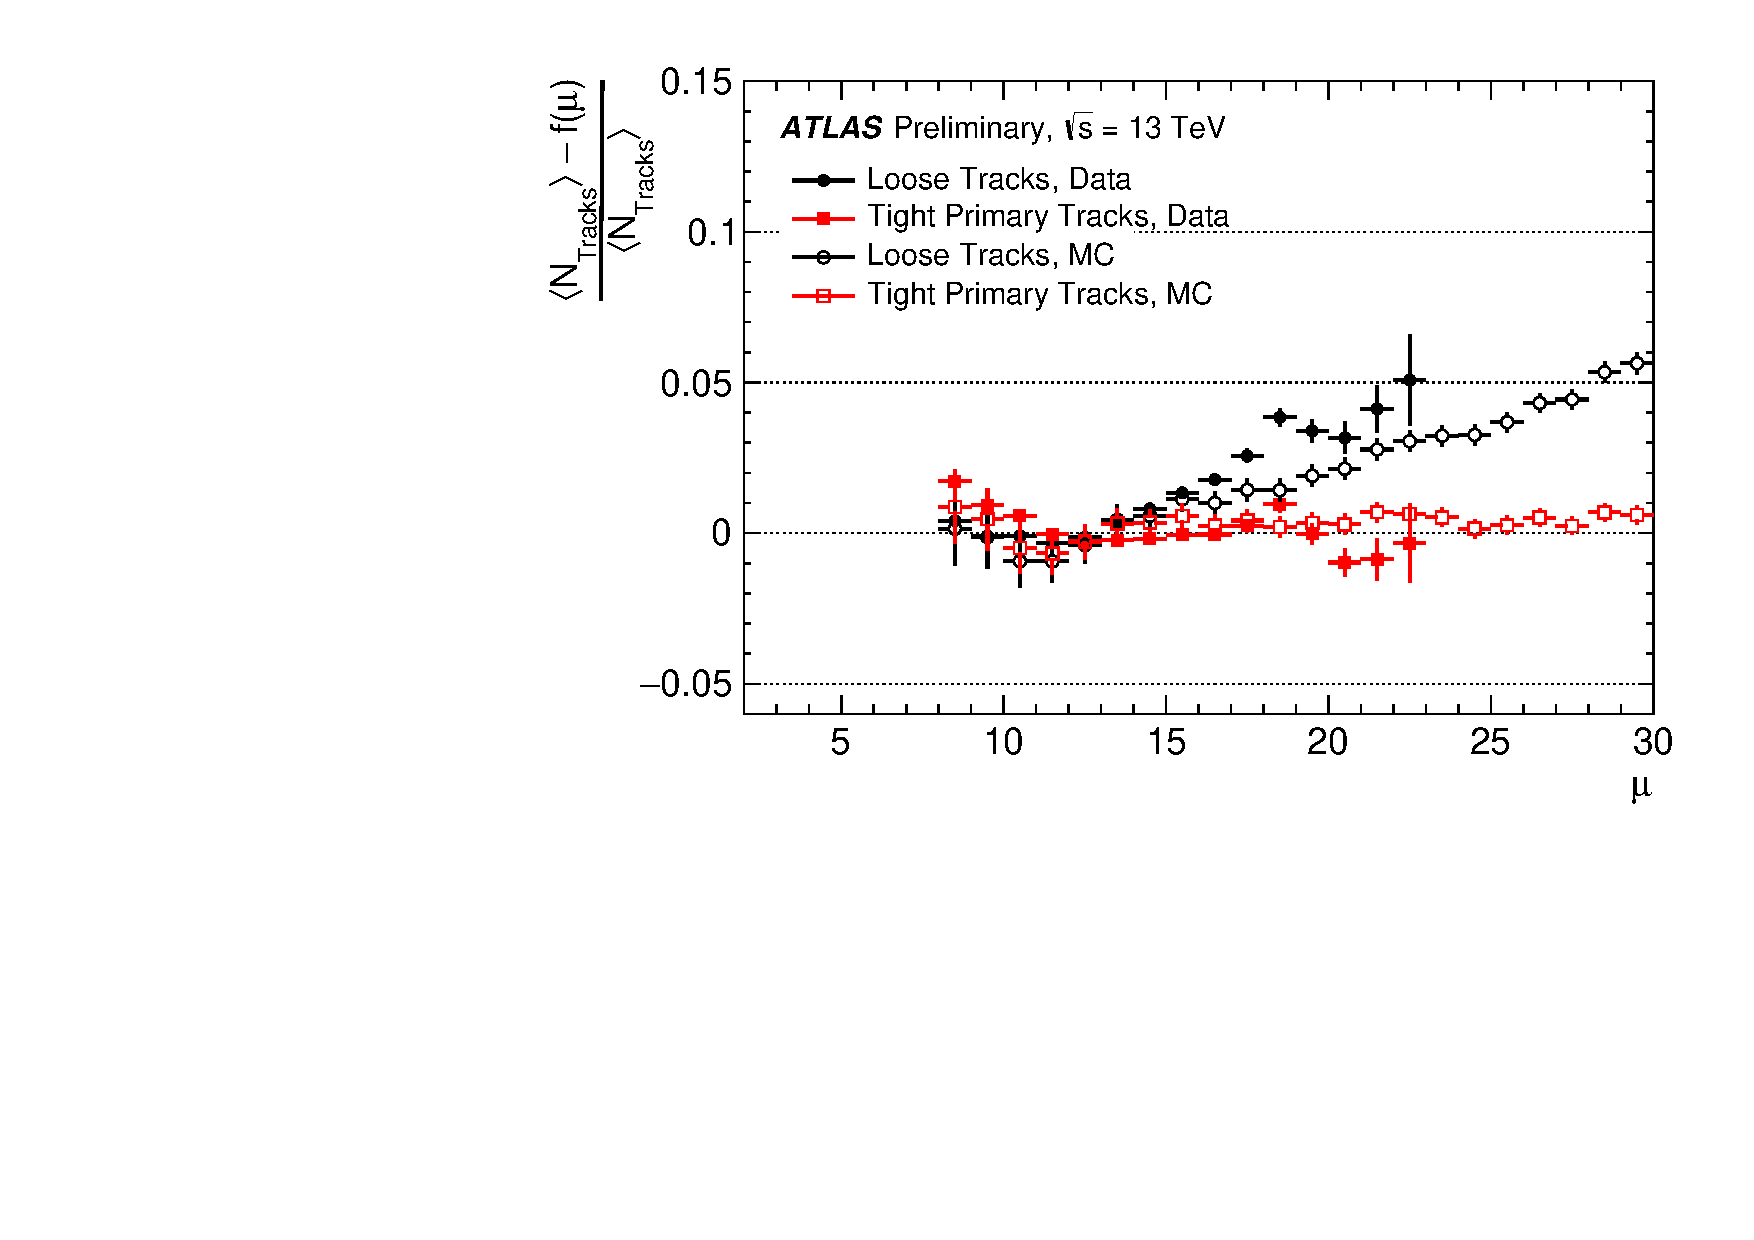
\includegraphics[width=0.55\linewidth]{figures/Reco/TrackingFake}
\caption{An estimation of the tracking fake rate, assuming the real tracks scale linearly as a function of $\mu$ for different track categories (Ref.\cite{ATL-PHYS-PUB-2015-051}). }
\label{fig:reco-trackingfake}
\end{center}
\end{figure}


The reconstructed tracks can help us find the event primary vertex, where the proton-proton hard scattering takes place. The set of tracks which are considered for vertices finding need to pass \cite{ATL-PHYS-PUB-2015-026}:

\begin{itemize}
\item $\pT > 400 \mev$
\item $|\eta|<2.5$
\item Number of silicon hits$>=$9 if $|\eta|\leq 1.65$
\item Number of silicon hits$>=$11 if $|\eta|>1.65$
\item At least 1 hit on IBL or B-layer
\item At most 1 shared module
\item No pixel holes
\item At most 1 SCT holes
\end{itemize}

%\begin{figure}[htpb!]
%\begin{center}
%  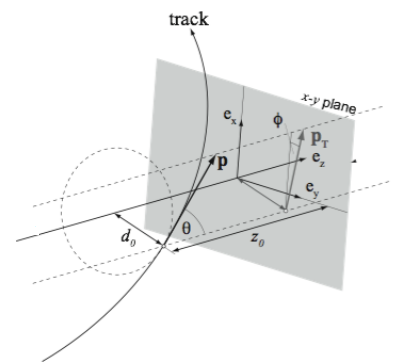
\includegraphics[width=0.55\linewidth]{figures/Reco/trackpar.png}
%\caption{Tracking parameter definitions. Tracks are parameterized by their five helix parameters. The $d_0$ and $z_0$ are the transversal and longitudinal impact parameters. The $\sigma(d0)=\frac{\d_0}{}$ and $\sigma(z0)$ are defined as the impact parameter significance
%\label{fig:reco-trkdef}
%\end{center}
%\end{figure}

The vertices finding algorithm, documented in \cite{PERF-2015-01}, starts with a seed position which is the mode of the z coordinates of all tracks. Knowing the seed, the algorithm iteratively calculates the vertex position by down-weighting the tracks which are far away and not compatible with this vertex. Each iteration re-calculates the vertex position. Tracks which are 7 $\sigma$ away are considered to not belong to this vertex and pooled for the iteration of finding the next vertex. Among all the vertices considered with at least two tracks associated to them, the one with highest track $\sum\pt^2$ is usually deemed as the primary vertex.

\begin{figure}[htpb!]
\begin{center}
  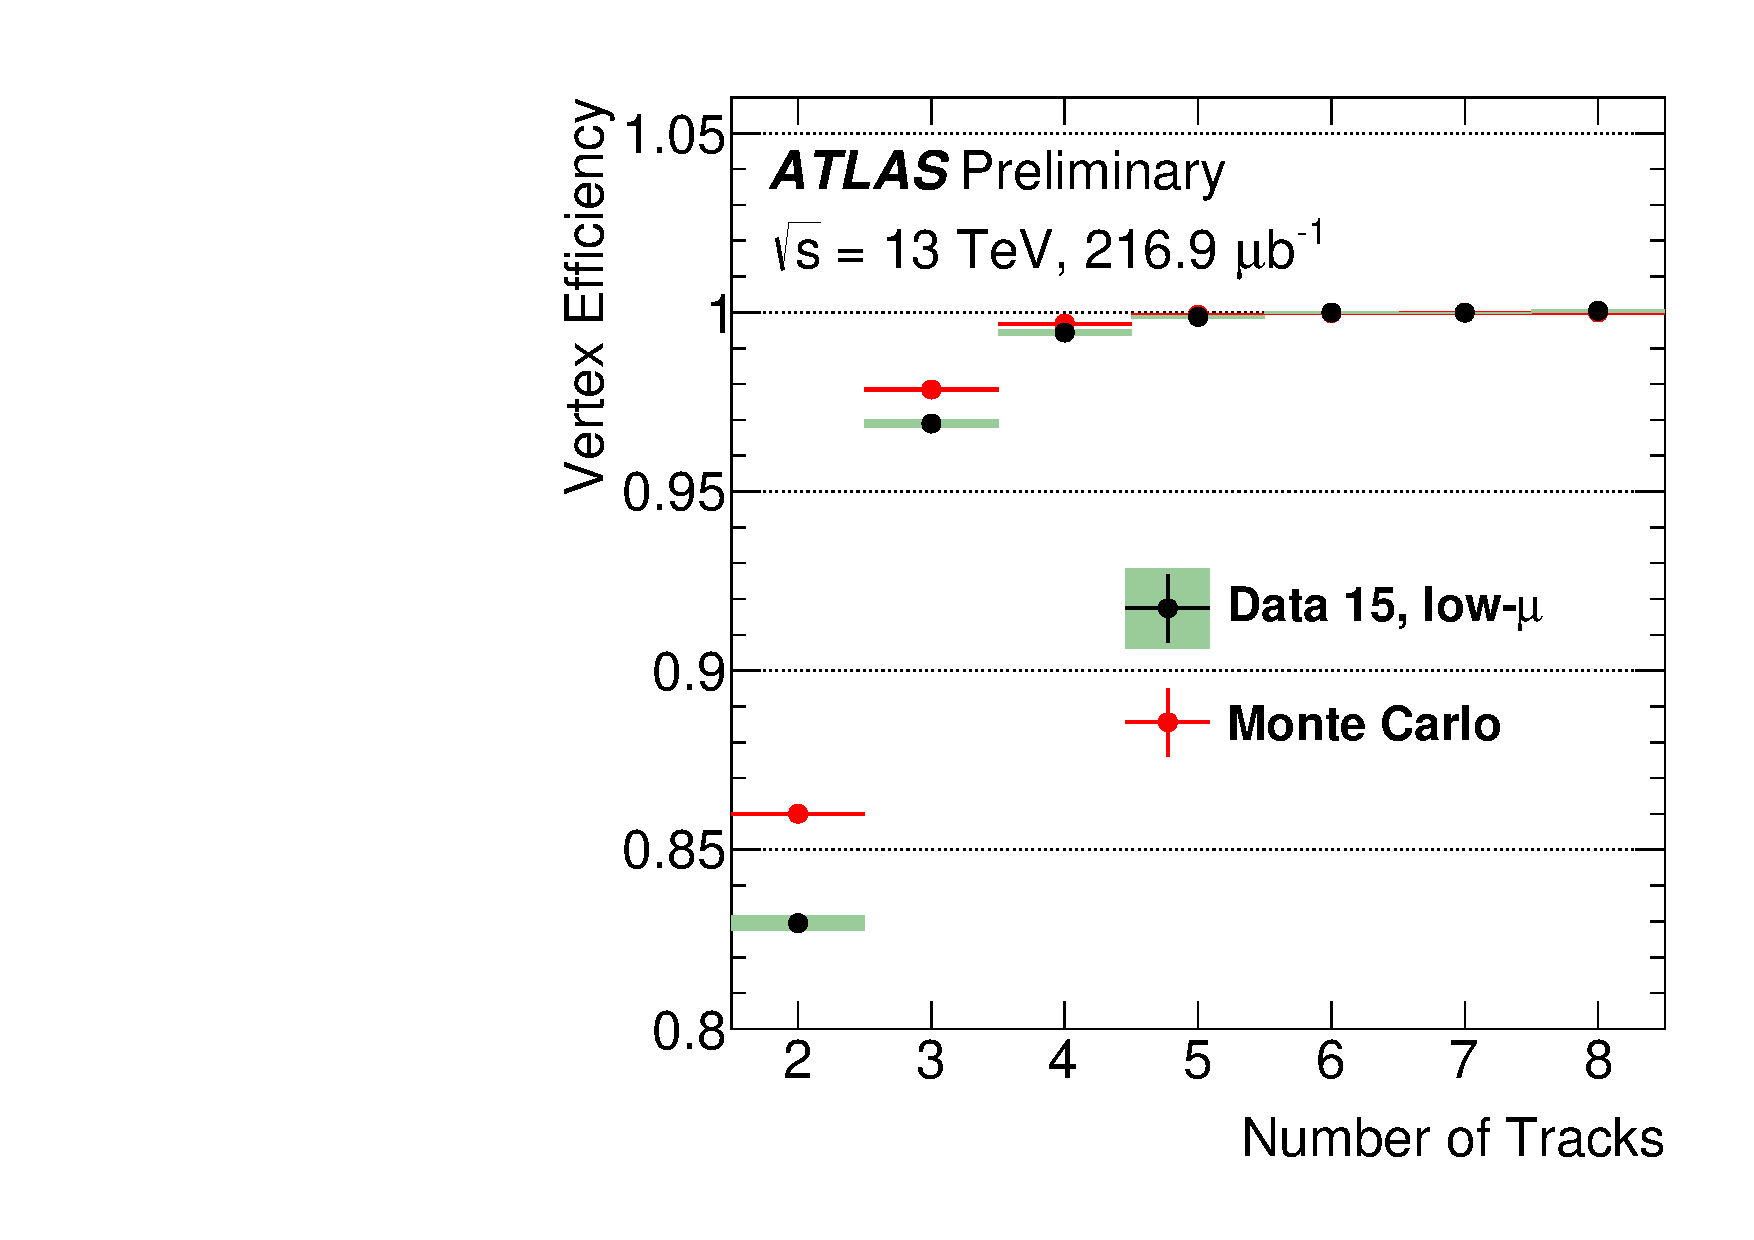
\includegraphics[width=0.55\linewidth]{figures/Reco/TrackingVertex}
\caption{Vertex reconstruction efficiency as a function number of tracks\cite{ATL-PHYS-PUB-2015-026}}
\label{fig:reco-primaryvertexeff}
\end{center}
\end{figure}




\section{Jets}
Energy deposits in calorimeter cells are first grouped into 3-D clusters called topological clusters (topocluster)\cite{PERF-2014-07}. We first form proto-clusters at the EM energy scale. The cells which pass a signal to noise significance $E/\sigma$  threshold are considred to belong to a cluster. The clustering algorithm starts with the seeds of significance$>4$ and then collects topologically connected (in the same layer adjacent or in two adjacent layers but have $\eta- \phi$ overlap) cells which are sig$>2$ and their direct neighbors with sig>0. Large clusters may lead to bad jet resolutions and are hence splitted if >=2 local maxima exists with $E^{EM}>500$ MeV with some spatial and layer constraints.

Many jet clustering algorithms exist. The most widely used algorithm within ATLAS is a sequential algorithm called $anti-kt$\cite{Cacciari:2008gp}. The jet shaped formed by this algorithm is not affected by soft radiations and making all the jet objects as conical. The algorithm treats clusters as input pseudo jets and calculates two metrics $d_ij$ and $d_iB$. If a pseudo jet is closer to the beam than to any other particle by these metircs then it is left alone. Otherwise it is combined with its nearest neighbor as as a single pseudo-jet adding together their momenta. The clustering algorithm continues untill no pseuodo jets can be combined.

As hadrnoic objects, jets require more dedicated correction of its four momenta than any other objects. ATLAS apply a series corrections\cite{PERF-2016-04} to jets in steps. First $|\eta|$ resolution is improved by using event primary vertex as jet origin. Pile-up contamination is corrected in the next step. Then MC based four momenta correction as well as jet initial composition corrections are applied. Jets in data also receive in situ callibration which corrects the difference between MC and data.


\clearpage

%%%%%%%%%%%%%%%%%%%%%%%%%%%%%%%%%%%
%%%%%  VBF
%%%%%%%%%%%%%%%%%%%%%%%%%%%%%%%%%%%
\chapter{VBF $h\rightarrow b\bar{b}$ Search with 2016 dataset}
\label{chap:vbf}
\section{Introduction}
As discussed in Chapter \ref{chap:intro}, the search of the Standard Model Higgs boson decaying to bottom quarks is essential in confirming the properites and the nature of the Higgs boson. The most sensitive production channel to study \Hbb is Vector Boson Associated (VH) production, as the requirement of having leptons or missing energies in the final state can reduce the background significantly. Most of the previous attempts to measure \Hbb were through the VH channel. Collaboratiely, the CDF and D0 experiments measured the \Hbb signal strength to be $\mu=\sigma/\sigma_\text{SM}=1.9 \pm 0.8$ ~\cite{Aaltonen:2012qt}. In the LHC era, Run I and early Run II combination of ATLAS and CMS experiments measured $\mu=0.90 \pm 0.27$ with a $3.6\sigma$ observed significance~\cite{HIGG-2016-29} and $\mu=1.1 \pm 0.3$ with a $3.8\sigma$ observed signifiance~\cite{CMS-HIG-16-044} respectively.

The Vector Boson Fusion (VBF) production mode serves as an orthogonal and complementary channel to the VH production, as the final states of the VBF \Hbb process are fully hadronic. Compared to Gluon-Gluon Fusion (ggF) production mode which also has fully hadronic final states but look very similar to generic multi-jet QCD processes, the VBF production has special event toplogies which can be exploited to surpress the QCD background. Since the Higgs bosns are Higgs bosons are color singlets with no color connection from other leading order final state particles to the decay product bottom quarks; little QCD radiation and hadronic activity is expected between the VBF jets, creating a rapidity gap between them. 

Using 20.2 \ifb~of data from 8~\tev~collisions, the ATLAS experiment measured a yield of -0.8$\pm$2.3 times the Standard Model predicted value\cite{HIGG-2014-12}. The CMS Collaboration released a result\cite{CMS-HIG-14-004} at \rts=8~\tev, and observed a fitted signal strength of $\mu = \sigma/\sigma_{SM} = 2.8^{+1.6}_{-1.4}$, corresponding to an observed significance of 2.2 standard deviations.   From combined measurements by both the ATLAS and CMS experiments\cite{HIGG-2015-07}, the measured signal strength for VBF production and the Higgs coupling to bottom quarks are $\mu_{\rm VBF}({\rm ATLAS+CMS})  = 1.18_{+0.25}^{-0.23}$ and $\mu_{bb} ({\rm ATLAS+CMS}) = 0.70^{+0.29}_{-0.27}$, respectively. The Run I VBF \Hbb results from both experiments are not very sensitive and conclusive and demonstrates the need of a continued study of this process. Due to the increase of the center of mass energy for the Run II LHC operation, the theoretical VBF Higgs production cross-section for mass at 125 \GeV increases by a factor of 2.3 from 8 to 13~\tev leading to a potentially more sensitive analysis than Run I. 

The overall strategy of the Run II VBF \Hbb analysis is fairly similar to that of Run I. The VBF \Hbb events have two $b$-jets and two VBF jets in the final states. Therefore, the event pre-selection starts from tagging two $b$-jets and requiring the events to have two more non $b$-tagged jets as documented in \ref{sec:vbf-objsel}. Two sets of the triggers target specifically for two different topologies in which either the two VBF jets are central (\fourcentral channel) or at least one VBF jet is in forward region (\twocentral channel) as described in \ref{sec:vbf-evtsel}. As documented in ~\cite{HIGG-2014-12}, Boosted Decision Tree (BDT) based analysis yields better overall sensitivity than cut-based analysis. This analysis adopted the BDT method to find most sensitive phase space to extract Higgs signal as described in \ref{sec:vbf-bdt}. The BDT is trained on simulated VBF signal events against backgrounds which are sidebands (events passing pre-selections with \Mbb in the region 80 \GeV~$< \Mbb<$~100 \GeV~ and  150 \GeV~$<$ \Mbb) of data events where the signals are depleted. The observed signal is extracted from a simultaneous fit to the \Mbb distribution in several regions defined by the event BDT scores with varying signal to background ratios. In each region\ref{sec:vbf-likelihood}, data is assumed to be the sum of non-resonant background (modeled with Bersnstein polynomials \ref{sec:vbf-nonres}), a resonant $Z$ contribution and a resonant Higgs contribution, both of which are parameterized by Bukin functions \ref{sec:vbf-parsigz}.

The Higgs mass window, i.e. the region 100 \GeV~$< \Mbb<$~140 \GeV, is kept blinded until the final profile likelihood fit is performed.  The fit strategy is validated first with a sideband-only fit to the $Z$ contributions, as described in Section~\ref{sec:vbf-zunblind}. The signal is extracted via a likelihood minimization where all relevant uncertainties are profiled and presented in Section~\ref{sec:vbf-higgsunblind}. Both the VBF process strength and the \Hbb process strength are measured. In Sec.~\ref{sec:vbf-higgscomb} the results are fit simultaneously with a related analysis (VBF$+gamma$), the search for Higgs decays to $b$-quarks in events enriched in VBF production with the additional requirement of a photon. Finally the combination results with other Higgs production and decay modes are shown in \ref{TODO}.


%In this analysis we cannot separate the VBF \Hbb and $ggF$ \Hbb contributions except during the BDT training, which is trained only on VBF events.  Thus all results are reported for the sum of the VBF and $ggF$ contributions.   Depending on the channel and region, the VBF and ggF contribution to the total Higgs signal varies significantly. In the most sensitive BDT regions, 81\% (\twocentral) and 82\% (\fourcentral) of the expected Higgs yield come from VBF production; while in the least sensitive regions, the ggF production dominate (77\% for \twocentral and 75\% for \fourcentral).


%This analysis is performed separately for two exclusive channels which correspond to the two trigger chains used to collect the data.  The \fourcentral channel requires four jets within $|\eta| < $2.8.  The \twocentral channel requires two central jets, and at least one jet with 4.4~$>|\eta|>$~3.2.  These channels are described in more detail in Section~\ref{sec:evtsel}. The kinematic properties of these jets are used as inputs to a boosted decision tree (BDT), described in Section~\ref{sec:bdt}.  The BDT is trained to classify events as signal-like or background-like.  

%Training signal events are taken from Monte Carlo (MC) simulation.  The background training uses events from data which pass the full event selection but have a Higgs candidate mass, \Mbb, 



\clearpage

\section{Datasets}
\subsection{Simulations}

The simulated samples used in this analysis are provided by the MC15c
production campaign of the ATLAS MC Production
Group \cite{TWiki_AtlasProductionGroup}. 
Simulated samples are used for the SM Higgs boson
ggF and VBF production, and strong and electroweak \zjets{} production.

For all signal samples, the detector response is simulated with the \geantFour{}
package~\cite{Agostinelli:2002hh}.
For the \zjets{} background samples, the detector response is simulated 
with the fast-simulation
package \atlfastTwo{}~\cite{Richter-Was:683751}.
Pile-up effects are taken into account by using minimum bias events
generated with \pythia{}~\cite{Sjostrand:2014zea} where the mean number of interactions
per bunch crossing is adjusted to the data-taking period.

VBF and ggF Higgs boson samples are generated with the next-to-leading order (NLO)
generator \powheg{}~\cite{Nason:2004rx,Frixione:2007vw,Alioli:2010xd} using the
CT10 PDF set~\cite{Lai:2010vv} and interfaced with \pythia{} for parton showering
and fragmentation with the AZNLO tune.
%Alternative samples, obtained by processing the same generated events with 
%\herwig{}~\cite{Bahr:2008pv,Bellm:2015jjp}
%for parton showering and fragmentation, are used for assessing modeling uncertainties.
We use two \zjets{} samples generated with \madgraph{}~\cite{Alwall:2014hca} 
using the NNPDF PDF set~\cite{nnpdf} and interfaced with \pythia{} for parton showering
and fragmentation with the A14 tune. One sample is used to model QCD $Z$ production.
In this sample electro-weak (EWK) production of $Z$
(e.g., $q+q \rightarrow W^{+} + W^{-} + qq  \rightarrow Z + qq$)
is explicitly not generated. To improve the efficiency of the sample
for our final state, two light partons (light quarks or gluons) are
required in the final state ($pp \rightarrow Z+ q/g + q/g$).
The second sample contains exclusively electroweak $Z$ production.
The cross sections of MC samples we use in this analysis are presented Table. \ref{tab:xsec}.

\begin{table}[htpb]
\centering
\caption{MC sample cross section times branching ratio}
\label{tab:xsec}
\begin{tabular}{|l|l|l|l|l|}
\hline
                   & VBF $h\rightarrow b \bar b$  & ggF $h\rightarrow b \bar b$  & QCD \zjets{} & EWK \zjets{} \\ \hline
$\sigma \times$ Br (Pb) & 2.22 & 25.91 & 666.52         & 4.86         \\ \hline
\end{tabular}
\end{table}

\subsection{Data}
We use 24.5~\ifb~of $13~\tev{}$ data recorded by the ATLAS detector in
2016. We use only the data that was collected during periods with all
detector subsystems were operational.  Additionally, the online transverse
beamspot position was required to be within 2mm of the nominal detector
center  due to the configuration of the $b$-jet trigger during this
period\footnote{
We use a special GRL from the ATLAS $b$-trigger group
\seqsplit{data16\_13TeV.periodAllYear\_DetStatus-v87-pro20-20\_DQDefects-00-02-04\_PHYS\_StandardGRL\_All\_Good\_25ns\_BjetHLT.xml}.}
%The luminosity determination is reported in Ref.~\cite{lumiwiki}.
The 2015 dataset is not used because the desired topology trigger chains were not available.

\clearpage

\section{Selections}
\subsection{Objects}
\label{sec:vbf-objsel}

The VBF \Hbb events have four jets in the final state.
The identification of the $b$-jets requires reconstruction of
{\it central} jets within the tracker coverage ($|\eta|<2.5$), while
the identification of forward VBF jets requires reconstruction
of {\it forward} jets with $2.5<|\eta|<4.4$. 


\subsubsection{Track and Primary Vertex Selection}

Several jet properties are computed using tracks associated to the jets. The tracks must pass the following selections:

\begin{itemize}
\item \pT $>$ 500 \mev
\item $|\eta| < $ 2.5
\item At least 7 silicon (pixel + SCT) hits
\item The sum the number of pixel hits shared with another track and half the number of SCT hits shared with another track must be less than 2
\item At most 2 missing silicon hits
\item At most 1 missing pixel hit
\item Track must be associated to the primary vertex, or $|z_0^{\rm PV}sin(\theta)| < 3$ mm  where $z_0^{\rm PV}$ represents the $z$ position of the track with respect to the primary vertex.
\end{itemize}

The track to jet matching is performed using ghost-association~\cite{GhostMatching,jetareas,atlasjetsub}, which provides a robust matching procedure that makes use of the area of the jet~\cite{GhostMatching}. In this procedure, the track four-vectors are used with track jet \pT set to an infinitesimal amount (the ``ghosts"), and re-clustering with calorimeter constituents is performed using the R=0.4 anti-$k_t$
algorithm.  Tracks which are clustered into the jet are then considered to be associated to the jet.  
The primary vertex is defined as the vertex in the event with the highest $\Sigma$ \pT$^2$ of the tracks associated to the vertex and at least two tracks.


\subsubsection{Jets}
\label{sec:vbf-jets}

%
%Jets are clustered with the anti-$k_t$
%algorithm~\cite{Cacciari200657,Cacciari:2008gp} (R=0.4) starting from
%topological clusters built from energy deposited in the
%calorimeter (AntiKt4EMJets). Jets are calibrated using a 
%simulation-based, energy and $\eta$ dependent
%calibration scheme, with in-situ corrections from data.~\cite{JESwiki}.
%
%The jet energy scale (JES) uncertainty is determined using residual
%uncertainties after the in-situ correction, with additional
%uncertainties including high-p$_T$ extrapolation and pile-up
%contributions.
%
%Jet quality criteria are applied to identify so-called~\textit{bad
%jets}, those not produced by in-time real energy deposits in the
%calorimeters, but instead caused by various sources including hardware
%problems in the calorimeter, LHC beam-gas interactions, and cosmic-ray
%induced showers. The jet quality criteria used for rejecting such jets
%follow the~\textit{Loose} selection detailed
%in~\cite{ATLAS-CONF-2015-029}. 

Jet reconstruction and calibration follows the description in Chapter \ref{chap:reconstruction}.
This analysis uses exclusively anti-$k_t$ R=0.4 jets.
Jets with $\pt < 60$ \GeV~and $|\eta| <$ 2.4 need to satisfy the
Jet Vertex Tagger, which is a pile-up jet rejection tool\cite{ATLAS-CONF-2014-018}, selection to ensure their origins are hard scattering vertices.
All jets are required to have $\pt>20$ \GeV and $|\eta|<4.4$.


\subsubsection{\bjets}

\label{sec:vbf-btagging}
The {\it MV2}-tagger as will be explained in Chapter \ref{chap:btagging} is used to identify \bjets. Specifically its variation {\it MV2c10} trained with $10\%$ $c$-jets in the training sample is used for this analysis.

%weights of three \btagging algorithms (JetFitter, IP3D and SV1) as
%well as $\pt$ and $\eta$ of the jet as an input to a neural network
% to determine a final tagging discrimination weight for each
%jet.
%Further details about the \btagging algorithms used can be
%found in \cite{Aad:2015ydr,ATL-PHYS-PUB-2016-012}.

Three different {\it MV2c10}-tagger operating points are considered, respectively with 60\% (tight), 70\% (medium) and 85\% (loose) tagging efficiency for jets
with $\pt > 20~\GeV{}$ and $\eta < 2.5$ as measured in semi-leptonic $t\bar{t}$ events. The corresponding light jet rejections vary from 1204 to 84 and the charm jet rejections vary from 6 to 150.

%The corresponding light jet, charm jet and tau rejection factors are detailed in Ref.~\cite{MV2c10wiki}.
%overall tagging efficiency of 70$\%$ and a
%corresponding light jet rejection factor of 381, charm jet
%rejection factor of 13 and a tau rejection factor of \btag
%55 \cite{MV2c10wiki} for jets with $\pt > 20~\GeV{}$ and $\eta < 2.5$. This working point is measured in a sample of \ttbar events.

In order to correct for differences in the \btagging performance between the data and MC simulation, per-jet scale factors are applied to the simulated jets and their product is taken as an event weight.
%\footnote{Currently, https://twiki.cern.ch/twiki/bin/view/AtlasProtected/BTagCalib2015\#Recommendation\_November\_2016 .  This will be updated before unblinding.}  

\subsubsection{Jet track distributions for quark/gluon separation}
\label{sec:vbf-qgtagging}

The VBF jets in the signal are expected to originate from a light quark, 
while in the backgrounds they primarily come from gluons.

The track multiplicity in the jet, \ntrk, is exploited to discriminate between quark- or gluon- initiated jets in the BDT, as gluon has larger color factor and hence larger average number of \ntrk. A dedicated study~\cite{qgtagging}  provides MC calibrations for the $n_{\rm track}$ distribution, as well as shape-based uncertainties.

%Gluons have a larger QCD color factor, and consequently their shower evolution produces more splittings. This property manifests itself in a larger per-jet particle multiplicity and a wider angular spread of the jet consituents.
%The $n_{track}$-based quark/gluon tagger~\cite{qgtagging} is used for jets with $\pT>50 \GeV$ and $|\eta|<2.1$.

\subsection{Event Selection}
\label{sec:vbf-evtsel}

The event selection targets two different signal topologies:
\begin{itemize}
\item \fourcentral: both VBF jets and \bjets from the Higgs decay are 
  found in the central region of the detector ($|\eta|<2.8$)
\item \twocentral: at least one VBF jet is required to be
  in the forward region ($|\eta|>3.1$)
\end{itemize}

These two categories are designed to be exclusive and are fed by two separate trigger paths.  

\subsubsection{Trigger Definitions}

\paragraph{\fourcentral:} Two triggers are used for this channel depending on the data taking periods. The pre-ICHEP dataset (data taking periods A-D of year 2016) uses HLT\_2j45\_bmv2c2070\_split\_2j45, which requires four central Level-1 jet objects, referred to as regions of interest (ROI),  with \ET $>$ 15 \GeV~( L1\_4J15).  In the HLT, two of these jets are required to have an HLT jet \ET of at least 45 \GeV~and be tagged with the 70\% working point of online $b$-tagging algorithm. The integrated luminosity of this pre-ICHEP trigger is 9.4~\ifb. Post-ICHEP (data taking periods E-L) due to the bandwidth limit, this analysis swtiched to using the HLT\_2J35\_bmv2c60\_2J35 trigger is used, which is seeded by the same L1 object.  In the HLT two of these jets are required to have an HLT jet \ET of at least 35 \GeV~and be tagged with the 60\% working point of online $b$-tagging algorithm. The integrated luminosity of this trigger is 13.3~\ifb.

\paragraph{\twocentral:} The HLT\_j80\_bmv2c2070\_split\_j60\_bmv2c2085\_split\_j45\_320eta490 is used for this channel for the entire dataset.  At L1, it requires at least one central jet with a Level-1 ROI \ET of 40 \GeV~and $|\eta| < 2.5$.  Additionally it requires another central jet with ROI \ET $>$ 25 \GeV~and a third, forward jet with ROI \ET of at least 20 and  $3.1 < |\eta| < 4.9$.   At the HLT one central jet \btagged  with the 70\% online working point with at least 80 \GeV~is required, in addition to a second jet with at least 60 \GeV~tagged at the looser 85\% working point. Lastly, the forward jet is required to have \ET $>$ 45 \GeV~at the HLT.


\subsubsection{Event Pre-Selection and Jet Assignment}
\label{sec:vbf-presel}

\paragraph{\fourcentral:} Events are required to pass the \fourcentral trigger depending on the data taking period. At least two offline jets with \pT $>$ 55 \GeV~and ($|\eta| < 2.5$) which pass the offline \btagging at the medium working point are required for the event to pass pre-selection.  These jets also have to be matched to the HLT trigger \btagged trigger objects. Two additional jets with \pT $>$ 55 \GeV~and  ($|\eta| < 2.8$) are also required. If there is a jet with \pT $>$ 60 \GeV~and 3.2 $< |\eta| <$ 4.4 the event is vetoed in order to avoid overlap with the \twocentral channel.

All pairs of \btagged jets passing the medium working point are considered and the high \pT  pair becomes our Higgs candidate.  All pairs of non-\btagged jets are also considered and the highest invariant mass pair form the VBF jets. Events in which the VBF jets pair cannot be formed are rejected.
%The VBF jet assignment fails where there are only four jets above the \pT threshold, of which three are $b$-tagged.
%These events are rejected. 

%Lastly, only events with a Higgs candidate transverse momentum, \pTbb, %of 
%greater than 150 \GeV~are considered.  This requirement is needed to remove kinematic sculpting of the \Mbb distribution in the low \Mbb region.  Figure~\ref{fig:mbb_ptcuts} shows the \Mbb distribution for a variety of \pTbb cuts for the  pre-selected events outside of the Higgs mass window (the background sample) for the \fourcentral channel on the left.  It can be seen that a broad ``bump" is present in the distribution between 200 and 300~\GeV~when no \pTbb cuts are applied.  

\paragraph{\twocentral:} Events are required to pass HLT\_j80\_bmv2c2070\_split\_j60\_bmv2c2085\_split\_j45\_320eta490.   We require at least one offline jet with \pT $>$ 95 \GeV~which is \btagged at the medium working point.  We also require at least one additional jet with \pT $>$ 70 \GeV~which passes the loose offline \btagging working point.  These two jets must be matched to the HLT \btagged objects.  In addition to these jets, at least one forward jet with \pT $>$ 60 \GeV~and 3.2 $< |\eta| <$ 4.4 is required.  Lastly, the event must have at least one more jet with \pT $>$ 20 \GeV~ and $|\eta| <$ 4.4.  

Jet assignment proceeds as follows.  All pairs of \btagged jets passing the loose working point which contain at least one jet passing the medium working point are considered and the highest \pT pair becomes our Higgs candidate.  The VBF jet candidates are formed from all pairs of jets passing pre-selection which are not part of the Higgs candidate pair,  including at least one of the forward jets from the pre-selection.  There is no requirement that these jets fail  the \btagging requirements. The highest invariant mass pair are labeled the VBF jets. 

%Lastly, only events with a Higgs candidate transverse momentum, \pTbb, greater than 160 \GeV~are considered.  This requirement is needed to remove kinematic sculpting of the \Mbb{} distribution in the low \Mbb{} region.  \Mbb{} is correlated with \pTbb{}, and the \pTbb{} distribution has a turn-on due to the jet \pT requirements. Figure~\ref{fig:mbb_ptcuts} shows the \Mbb distribution for a variety of \pTbb cuts for the background sample for the \twocentral channel on the right.  As the \pTbb{} cut is increased, the distribution assumes a regular falling spectrum.  The sculpting is worse for the \twocentral channel than the \fourcentral channel due to the higher threshold jet requirements.


\paragraph{\pTbb cut:} Common to both channels is a \pTbb cut applied at the last step of pre-selection. As shown in Fig. \ref{fig:vbf-mbb_ptcuts}, the jet trigger and kinematic requirements sculpt the \Mbb distribution. A \pTbb cut at 150\GeV and 160\GeV is applied to \fourcentral and \twocentral channels smooth the \Mbb distribution.

\begin{figure}[htbp]
  \centering
 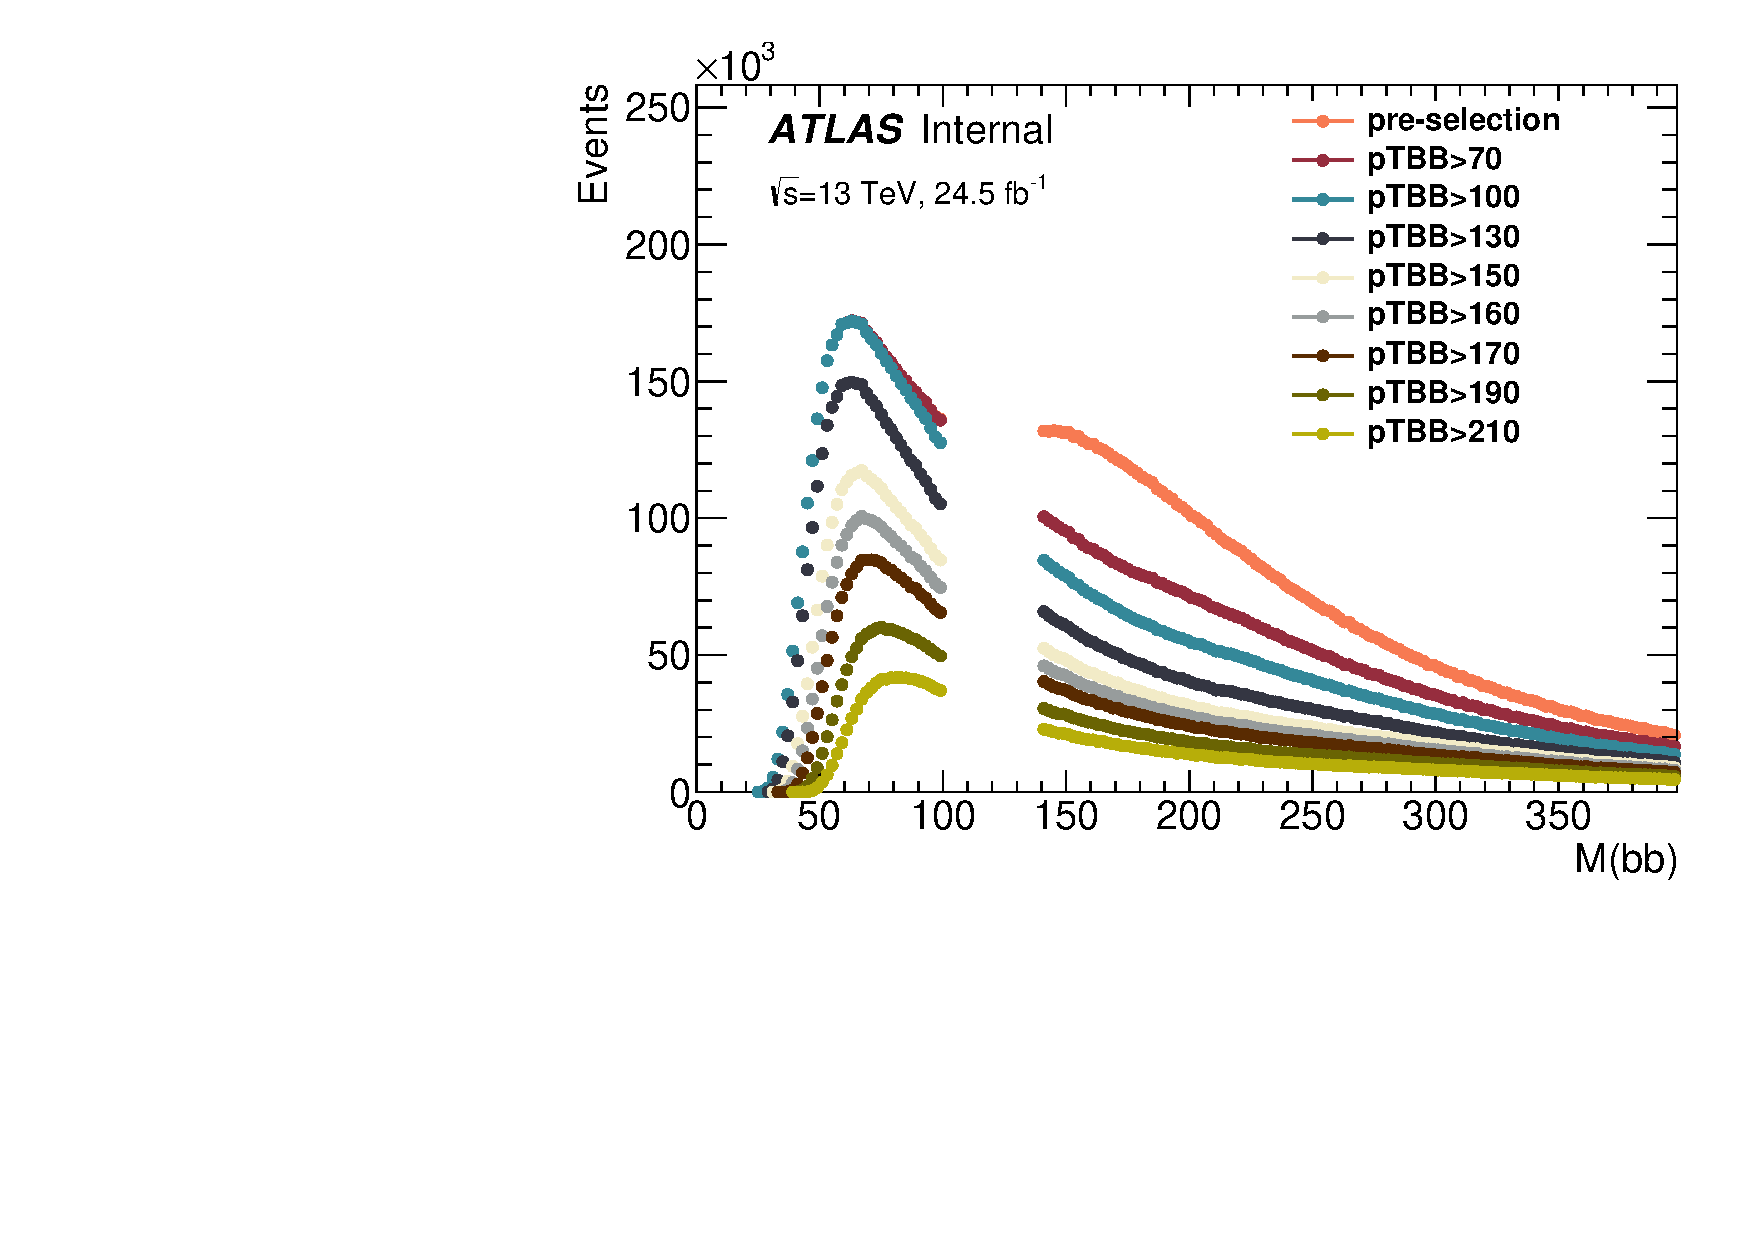
\includegraphics[width=0.45\textwidth]{figures/VBF/Presel-Mbb_4cen.pdf}
 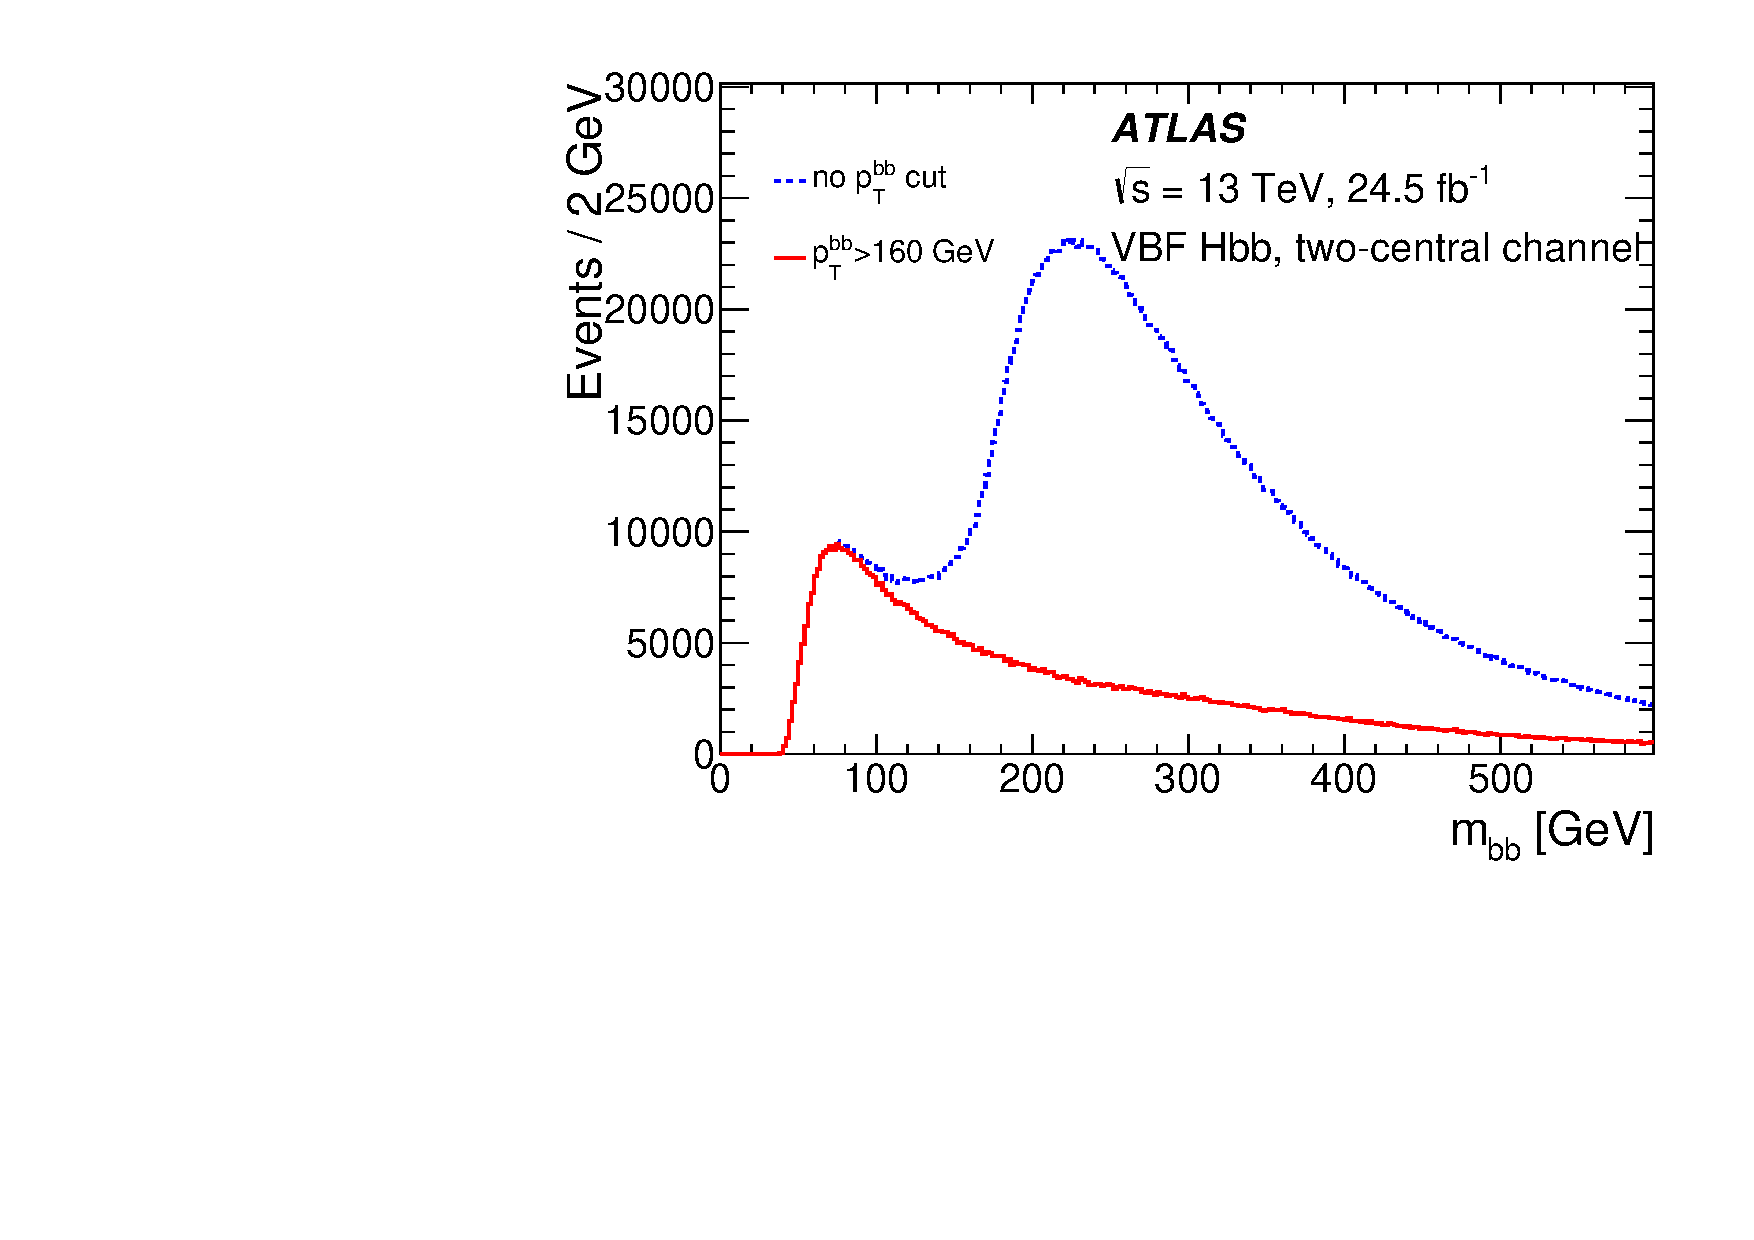
\includegraphics[width=0.45\textwidth]{figures/VBF/Presel-Mbb_2cen.pdf}
 \caption{Distributions of \Mbb for a variety of \pTbb cuts using data events.  \fourcentral events on the left, \twocentral on the right.  All event pre-selection criteria except the \pTbb cuts are applied.}
  \label{fig:vbf-mbb_ptcuts}
\end{figure}


%\paragraph{0-tag samples:} Both the \fourcentral and \twocentral channels have corresponding 0-tag samples in which the offline jets are required to be anti-\btagged at the 85\% working point. These samples are used to determine the sensitivity when determining the signal and control BDT regions.   A relatively tight anti-tag is required in order to minimize any leakage of the signal into the 0-tag sample.  In these samples supporting triggers are used, which have the same Level-1 and HLT jet requirements, but no \btagging requirements.  These triggers are heavily pre-scaled.  

\paragraph{Overlap with VBF$+\gamma$ Analysis:} The result of this analysis is eventually combined with the complementary VBF$+\gamma$ analysis which studies the same event topology with an additional photon radiated by the initial/final state quarks or the vector bosons. For the two analyses to remain orthogonal, the inclusive analysis vetos events selected by the VBF$+\gamma$ analysis in data. From simulation it is determined that only 0.11\% and 0.047\% of the inclusive VBF signal MC would pass selections of both analyses given that they pass \twocentral and \fourcentral respectively. The size of this overlap is so small, less than $0.5\%$ (a criterion for us to account a particular source of systematics in the final fit \ref{sec:vbf-uncertainties}), such that it is neglected.  

%Then put into BDT & we have SR1, SR2 & CR.  Used to have 0 tag control sample but not used.
%The details of the event selection are summarized in Table~\ref{tab:evtsel}. 
%With exception of the trigger requirements, the same requirements are placed on the data and MC samples.  In the MC15 samples the trigger decision is missing for the \twocentral channel, therefore an alternative emulation is used, described briefly in Section~\ref{sec:vbf-trig}.


The details of the event selection are summarized in Table~\ref{tab:evtsel}. 
Jet \pT thresholds and $|\eta|$ requirements are chosen so that the efficiency of selecting a jet at trigger level that would pass the offline selection is at least 97\%. Cut flows for both selections are displayed in Tables~\ref{tab:cutflow_4cen} and~\ref{tab:cutflow_2cen}.


\begin{table}[htbp]
  \begin{center}
    \resizebox{\textwidth}{!}{
      \begin{tabular}{ l  c c }
        \toprule
        & \fourcentral & \twocentral \\
        \midrule
        L1 trigger          & L1\_4J15                 & L1\_J40\_0ETA25\_2J25\_J20\_31ETA49                                \\
\\
        Primary HLT trigger  & HLT\_2j45\_bmv2c2070\_split\_2j45  & HLT\_j80\_bmv2c2070\_split\_j60\_bmv2c2085\_split\_j45\_320eta490  \\ 
                 & HLT\_2j35\_bmv2c2060\_split\_2j35  &   \\ 

      \\ 
        Support HLT trigger & HLT\_4j45                          & HLT\_j80\_0eta240\_j60\_j45\_320eta490                             \\ 
        \\
                                              &                                                     & $\geq4$ jets with $\pt>20$ \GeV{} and $|\eta|<4.4$ \\
                                              &                                                     & $\geq1$ jet with $\pt>60$ \GeV{} and $3.2<|\eta|<4.4$  \\ 
                                              &                                                     & $\geq2$ jets with $\pt>70$ \GeV{} and $|\eta|<2.5$ \\ 
        \multirow{-4}{*}{Jet selection}       & \multirow{-4}{*}{$\geq4$ jets with $\pt>55$ \GeV{} and $|\eta|<2.8$} & $\geq1$ jet with $\pt>95$ \GeV{} and $|\eta|<2.4$  \\ 
        \\
        
        \multirow{2}{*}{$b$-tagging}          & \multirow{2}{*}{$\geq2$ $b$-jets with $\pt>55$ \GeV{} and $|\eta|<2.5$} & $\geq2$ $b$-jets with $\pt>70$ \GeV{}                  \\ 
                                              &                                                        & $\geq1$ $b$-jets with $\pt>95$ \GeV{} and $|\eta|<2.4$ \\ 
        Forward jet veto                      &   No jet with $\pt>60$ \GeV{} and $3.2<|\eta|<4.4$    &  \\ 
        Higgs boson candidate                 &       $\pt(b\bar{b})>150$ \GeV{}                       &  $\pt(b\bar{b})>160$ \GeV{} \\  
        
        \bottomrule
      \end{tabular}
    }
  \end{center}
  \caption{Event selection for the two event categories. The \fourcentral has two primary trigger paths.  The first is used for the pre-ICHEP dataset, the second is used for the post-ICEP dataset. \bjets{} are tagged with the 70\% working point and are required to have $|\eta| < 2.5$}
  \label{tab:evtsel}
\end{table}




\begin{table}[]
\centering

\begin{tabular}{|l|l|l|l|l|l|}
\hline
                       & \multicolumn{5}{c|}{Pre-ICHEP}                                 \\ \hline
                       & data 2tag  & VBF       & ggF        & Zbb(QCD)     & Zbb(EWK)  \\ \hline
Events                 & 122517049* & 20127.8 & 234762.8 & 3880727.1    & 29277.8 \\ \hline
Trigger                & 29623250   & 627.0    & 2192.1    & 98931.1    & 1444.5  \\ \hline
2 medium \btagged jets & 13910362   & 334.3    & 1207.3    & 45110.5    & 705.0    \\ \hline
$\ge$ 4 jets           & 9255271    & 215.2    & 892.1     & 35903.9    & 566.7    \\ \hline
Forward jet veto       & 9021208    & 205.8    & 869.9     & 34675.7    & 545.1    \\ \hline
Jet Assignment         & 8290467    & 197.2    & 820.2     & 33604.2    & 532.1    \\ \hline
$\pTbb>150\GeV$        & 3146579    & 121.8    & 532.4     & 21084.0    & 379.2    \\ \hline
Photon veto in data    & 3145966    & 121.8    & 532.4     & 21084.0    & 379.2    \\ \hline
                       & \multicolumn{5}{c|}{Post-ICHEP}                                \\ \hline
                       & data 2tag  & VBF       & ggF        & Zbb(QCD)     & Zbb(EWK)  \\ \hline
Events                 & 169139398* & 28565.5 & 332929.0 & 5505804.9 & 41551.4 \\ \hline
Trigger                & 43820814   & 1024.1   & 3602.9    & 166327.2   & 2271.5  \\ \hline
2 medium \btagged jets & 19370468   & 501.8    & 1868.4    & 64549.5    & 955.6    \\ \hline
$\ge$ 4 jets           & 10218887   & 273.8    & 1133.7    & 45143.9    & 712.8    \\ \hline
Forward jet veto       & 9963404    & 261.9    & 1105.7    & 43605.2    & 685.1    \\ \hline
Jet Assignment         & 9065632    & 250.2    & 1037.5    & 42163.0    & 667.9    \\ \hline
$\pTbb>150\GeV$        & 3755031    & 158.0    & 685.4     & 27202.8    & 486.5    \\ \hline
Photon veto in data    & 3754301    & 158.0    & 685.4     & 27202.8    & 486.5    \\ \hline
\end{tabular}
  \caption{Cutflow for the \fourcentral events.  MC events are normalized to cross section times branching ratio.  The total number of data events is after the application of the derivation skimming whereas the MC events are the total number of events in the MC samples. *The data number of total events is the number of all events after the derivation skim.}
  \label{tab:cutflow_4cen}
\end{table}


\begin{table}[]
\centering
  
\begin{tabular}{|l|l|l|l|l|l|}
\hline
                            & data       & VBF       & ggF       & Zbb(QCD)    & Zbb(EWK)    \\ \hline
Events                      & 291656447* & 52628.6 & 613382.5 & 10143797.6 & 76540.4    \\ \hline
Trigger                     & 18425823   & 679.2    & 594.0    & 23942.1    & 555.7      \\ \hline
1 Medium \btagged jet       & 10321971   & 455.0    & 405.2    & 14816.1    & 369.6      \\ \hline
$\ge$ 2 loose \btagged jets & 3529025    & 269.7    & 244.5    & 7753.0     & 203.9      \\ \hline
Forward jet requirement     & 2814936    & 214.9    & 181.6    & 5328.1     & 162.7      \\ \hline
$\ge$ 4 jets                & 2527300    & 208.1    & 176.0    & 5307.6     & 161.7      \\ \hline
Jet Assignment              & 2527300    & 208.1    & 176.0    & 5307.6     & 161.7      \\ \hline
$\pTbb>160\GeV$             & 884095     & 147.3    & 126.5    & 3565.7     & 122.4      \\ \hline
Photon veto in data         & 883906     & 147.3    & 126.5    & 3565.7     & 122.4      \\ \hline
\end{tabular}
   \caption{Cutflow for the \twocentral events. MC events are normalized to cross section times branching ratio. The total number of data events is after the application of the derivation skimming whereas the MC events are the total number of events in the MC samples. *The data number of total events is the number of all events after the derivation skim.}
   \label{tab:cutflow_2cen}
\end{table}


\subsection{Event Weights}
In order to compare with the distributions observed in data, the simulated samples are normalized
to the number of events expected based on the theoretical cross section and the integrated luminosity.
An event weight $w_{MC}$ is applied, defined as:
\begin{equation}\label{eq:mcweight}
w_{MC} = \frac{\sigma\times k}{N} L,
\end{equation}
where $\sigma$ is the theoretical cross section for the process considered, $N$ is the
number of simulated events, $L$ the integrated luminosity and $k$ a
correction to the LO cross section to reproduce a higher--order
(e.g. NLO) calculation for the process of interest.

In addition, a weight is applied  to account for the pile--up
conditions in data. While events are generated for the whole spectrum
of number of interactions per bunch crossing $<\mu>$, the proportions
are not the same as in data. The pile--up weight, $w_{PU}$ ensures that the
$<\mu>$ distribution in simulated samples matches the one in data.

To ensure an accurate modeling of the detector effects, reconstruction
and selection efficiencies $\epsilon$ are calibrated with {\it scale factors}
(SF) defined as 
\begin{equation}
SF = \frac{\epsilon_{data}}{\epsilon_{MC}},
\end{equation}
where $\epsilon_{data}$ and $\epsilon_{MC}$ are measured in dedicated
data calibration samples and in the equivalent MC simulation, respectively.
We apply scale factors for offline \btagging, JVT and \ntrk. 

We apply efficiency scale factors to jets which pass the offline \btagging working point in simulated events. 
The scale factors of \bjets and $c-$jets are derived from $t\bar t$ events while scale factors of light jet are derived from di-jet events. 
We also apply inefficiency scale factors to jets which fail \btagging. The total \btagging weight, $w_{b-tag}$, is calculated as the product of the scale factors of all jets passing the preselection. Similarly per-jet SFs are applied for JVT efficiency and \ntrk for all jets passing the preselection and we multiply the SFs to get JVT and \ntrk weights $w_{JVT}$ and $w_{\ntrk}$.

The online \btagging and offline \btagging use the same tagging algorithm but different track collections. 
We correct the simulated event weights by the ratio (scale factor) of online b-tagging efficiency with respect to offline b-tagging efficiency at different working points. 
The scale factors are parameterized as a function of online \bjet $p_T$ and measured in $t\bar t$ events. 
The trigger weight is calculated as $w_{trig} = \prod_{i} SF(p_T)_{i}$, where $SF(p_T)_i$ denotes the scale factor of $i^{th}$ signal jet matched to an online b-jet of a given $p_T$. 

The final event weight of a simulated event is $w = w_{MC}\times w_{PU} \times w_{b-tag} \times w_{JVT} \times w_{\ntrk} \times w_{trig}$. 




\clearpage

\section{Multi-variate Analysis}
\label{sec:vbf-bdt}

\subsection{BDT Input and Training}
Evets passing the pre-selections are fed into Boosted Decision Tree (BDT) to find phase space with high signal purity.
The BDT is trained with scikit-learn package~\cite{scikit-learn}.
The classifier has 200 trees and employs the AdaBoost method.
The background sample is taken from data events with $80~\GeV < \Mbb <100$~\GeV~
and $150~\GeV<\Mbb<190$~\GeV~and contains approximately 690k events for
the \fourcentral channel and 90k events for the \twocentral channel.
The signal contamination in this region is negligible.
The $Z$ contribution to the low-mass sideband is not explicitly accounted
for due to its small size (see Tables~\ref{tab:cutflow_4cen}
and~\ref{tab:cutflow_2cen} for the number of events of each type passing pre-selection).
As will be shown in Figure~\ref{fig:vbf-BDTResponse},
the BDT response of the QCD-produced \zjets~ sample is very similar to the background samples. 

The signal sample is the VBF Monte Carlo simulated dataset and
contains 10k events for the \fourcentral channel and 2k events for
the \twocentral channel.  Half of the signal and background samples are
used for training and the other half are used for validation.

The following variables are used for training:
\begin{enumerate}
\item $M_{\rm JJ}$, the invariant mass of the VBF jet pair. 
\item $p_{\rm T,JJ}$, the transverse momentum of the VBF jet pair. 
\item $\cos{\theta}$, cosine of the polar angle of the cross product of the momenta of the VBF jets in the Higgs boson's rest frame.
\item $Max (\eta)$, the maximum between the absolute values of the pseudo-rapidity of the VBF jets: $Max (\eta) \equiv max( |\eta_{J1}|, |\eta_{J2}| )$
\item $\eta* = \frac{1}{2}( |\eta_{\rm J1}| + |\eta_{\rm J2}| - |\eta_{\rm B1}| - |\eta_{\rm B2}|)$, average pseudo-rapidity difference between VBF and signal jets.
\item $min\Delta R$(J1), minimum angular separation between the leading VBF jet and its closest jet. 
\item $min\Delta R$(J2), minimum angular separation between the sub-leading VBF jet and its closest jet. 
\item QGTagger(J1),  the number of tracks associated to the leading VBF jet, as described in Section~\ref{sec:vbf-qgtagging}.
\item QGTagger(J2),  the number of tracks associated to the sub-leading VBF jet, as described in Section~\ref{sec:vbf-qgtagging}.
\item $p_{T}$ balance, the ratio of vectorial and scalar sum of signal and VBF jets \pT,  $\frac{\overrightarrow{p_{T}}(J1)+\overrightarrow{p_{T}}(J2)+\overrightarrow{p_{T}}(B1)+\overrightarrow{p_{T}}(B2) }{ p_{T}(J1)+p_{T}(J2)+p_{T}(B1)+p_{T}(B2)}$
\item $\Delta M_{\rm JJ}$, the difference between largest invariant mass calculated using all jet pairs and only VBF jet pair. 
\end{enumerate}

The distributions of all input variables for each channel are
shown in Appendix\ref{sec:app-vbf-inputs}.
The correlation between the input variables and the \Mbb value of the event
is examined to ensure that the variables chosen will not create artificial
structures in the \Mbb distribution.
As shown in Figure~\ref{fig:vbf-BDTInputsCor}, most variables have a
small correlation factor of less than 0.1 with \Mbb. 
The BDT response of lower and upper data sidebands are checked and no obvious
mass dependece is observed as shown in Figure\ref{fig:vbf-bdtsidebands}.

\begin{figure}[htbp]
  \centering
 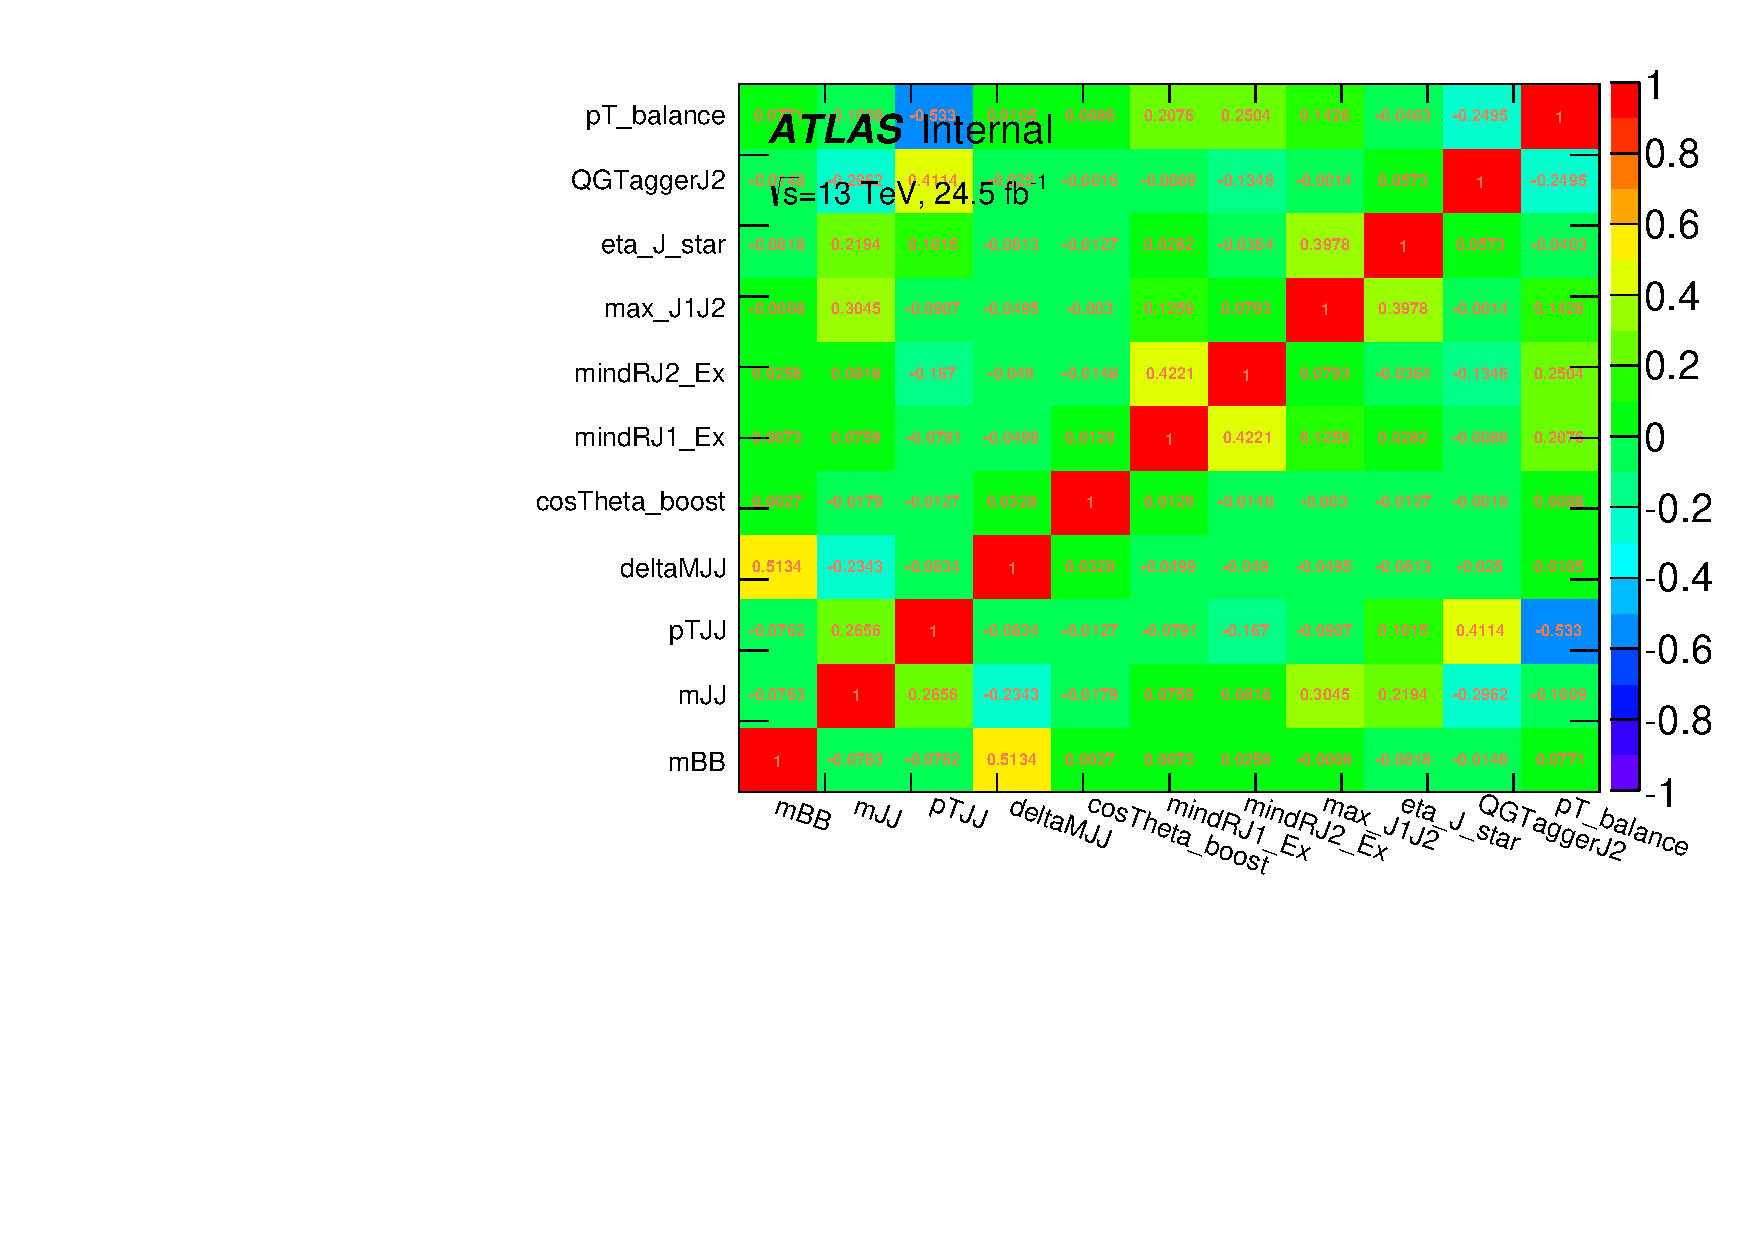
\includegraphics[width=0.48\textwidth]{figures/VBF/BDT_VBF_var_cor_2cen.pdf}
 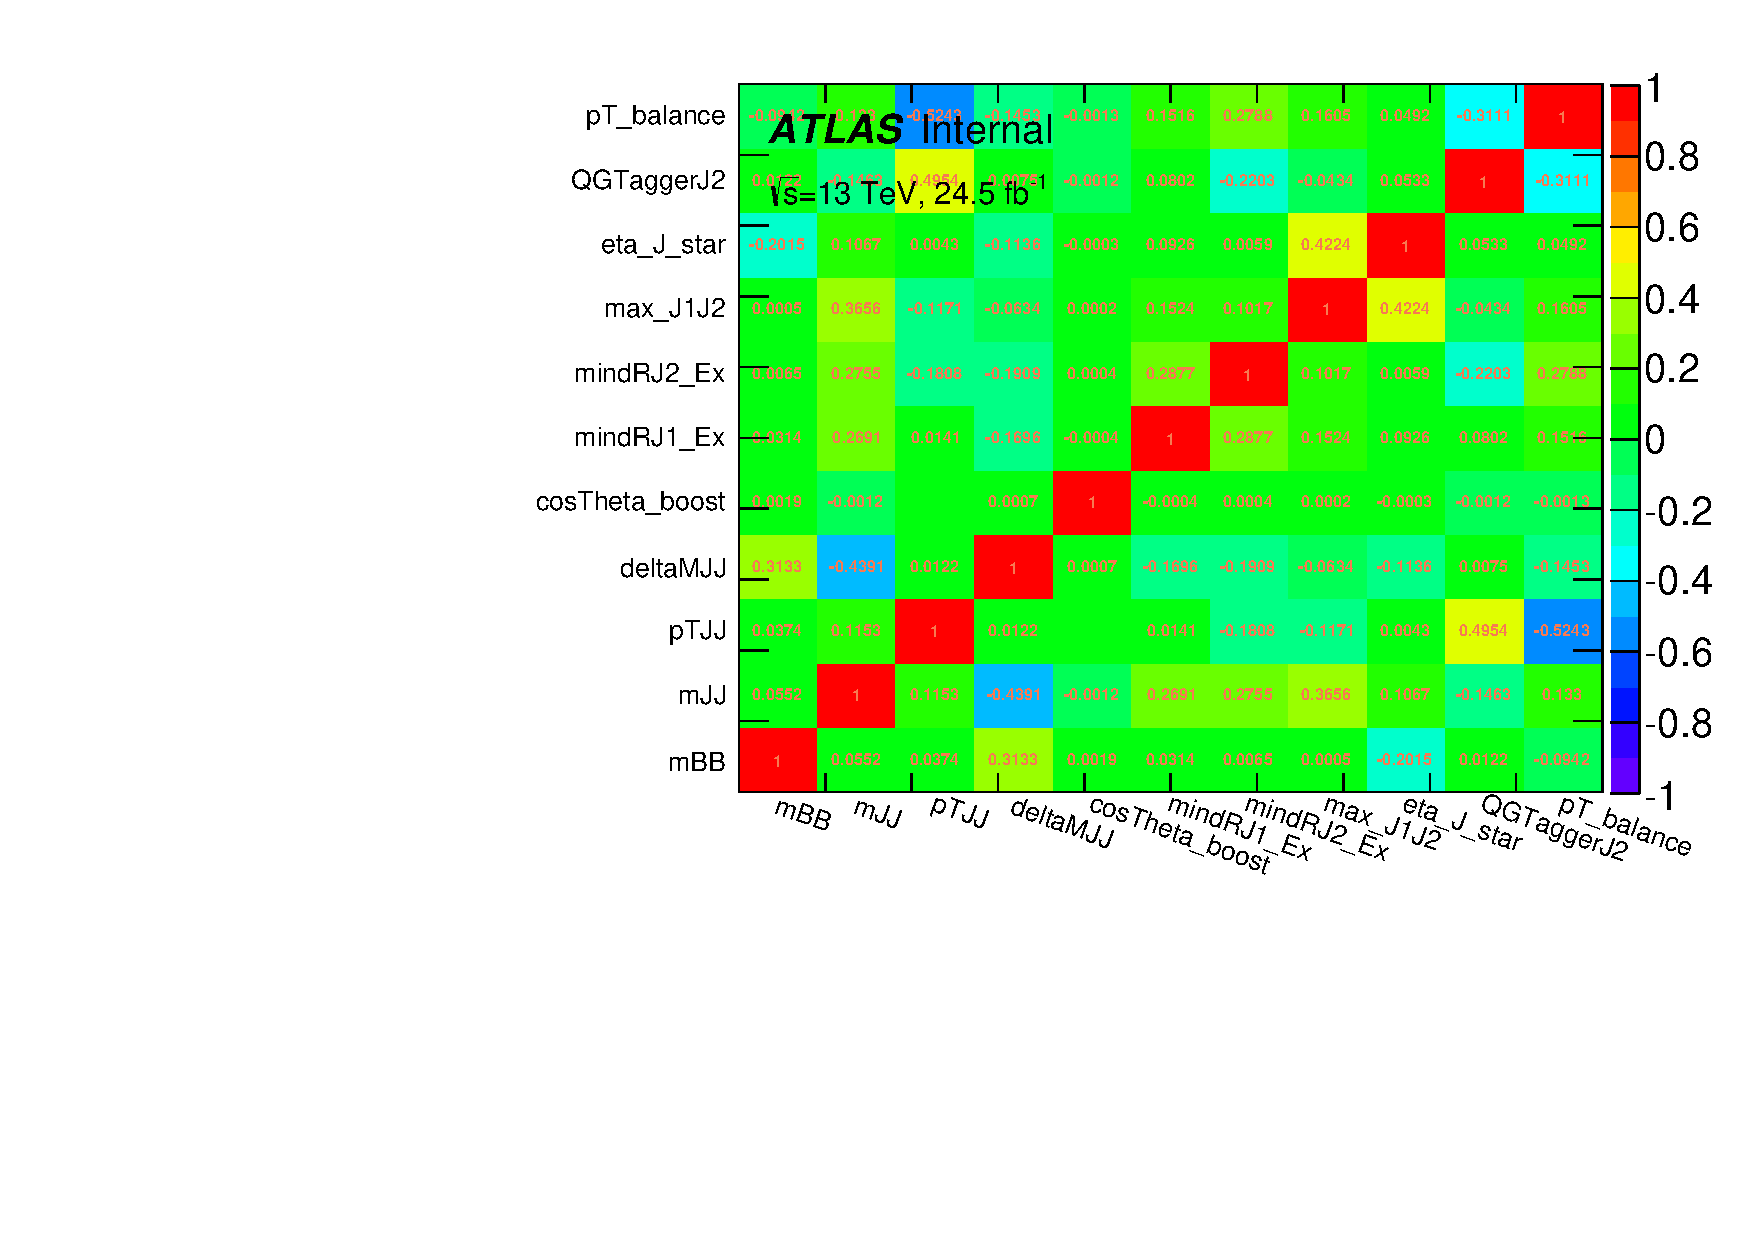
\includegraphics[width=0.48\textwidth]{figures/VBF/BDT_data_var_cor_2cen.pdf}\\
 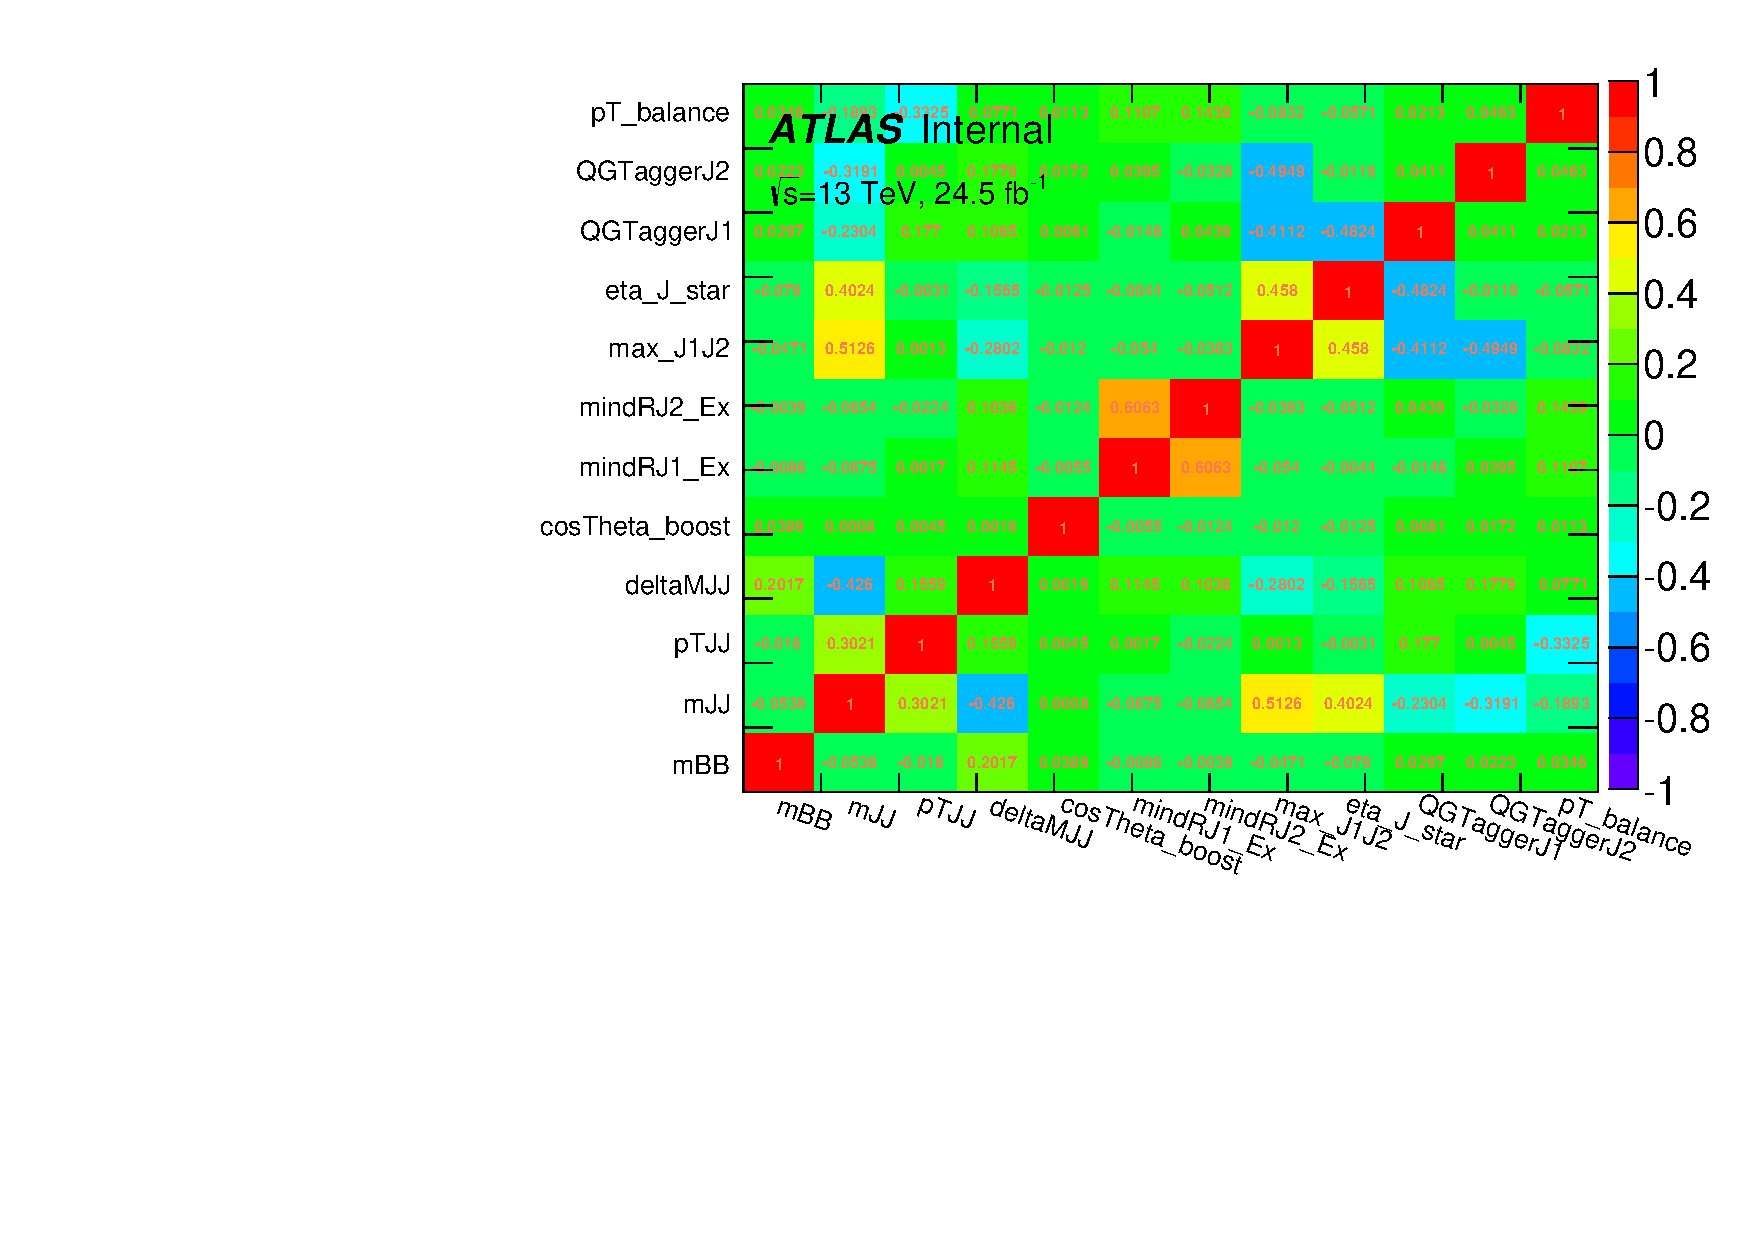
\includegraphics[width=0.48\textwidth]{figures/VBF/BDT_VBF_var_cor_4cen.pdf}
 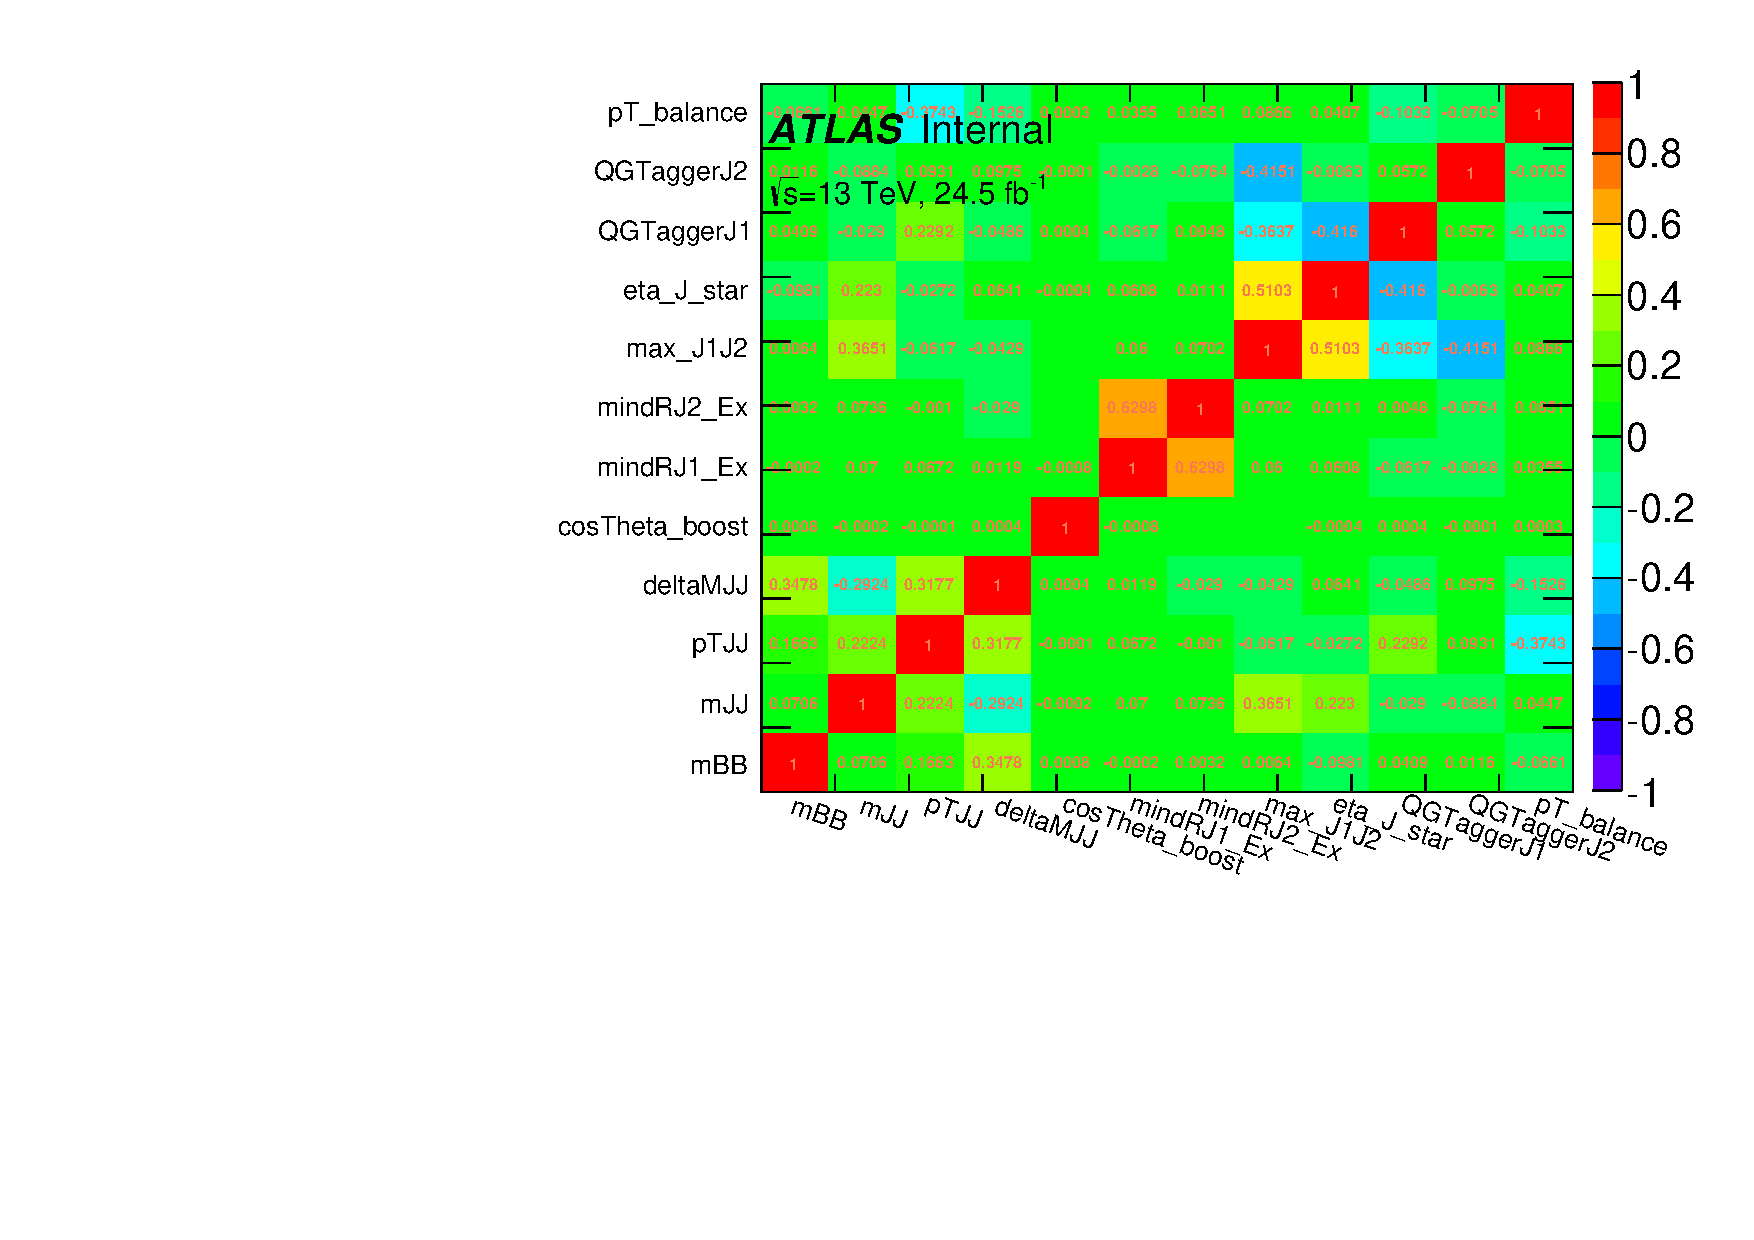
\includegraphics[width=0.48\textwidth]{figures/VBF/BDT_data_var_cor_4cen.pdf}\\
\caption{Correlations between BDT input variables and $\Mbb$ of signal (left) and background (right) of  the \twocentral (top) and \fourcentral (bottom) channels.}
  \label{fig:vbf-BDTInputsCor}
\end{figure}


\begin{figure}[htbp]
  \centering
 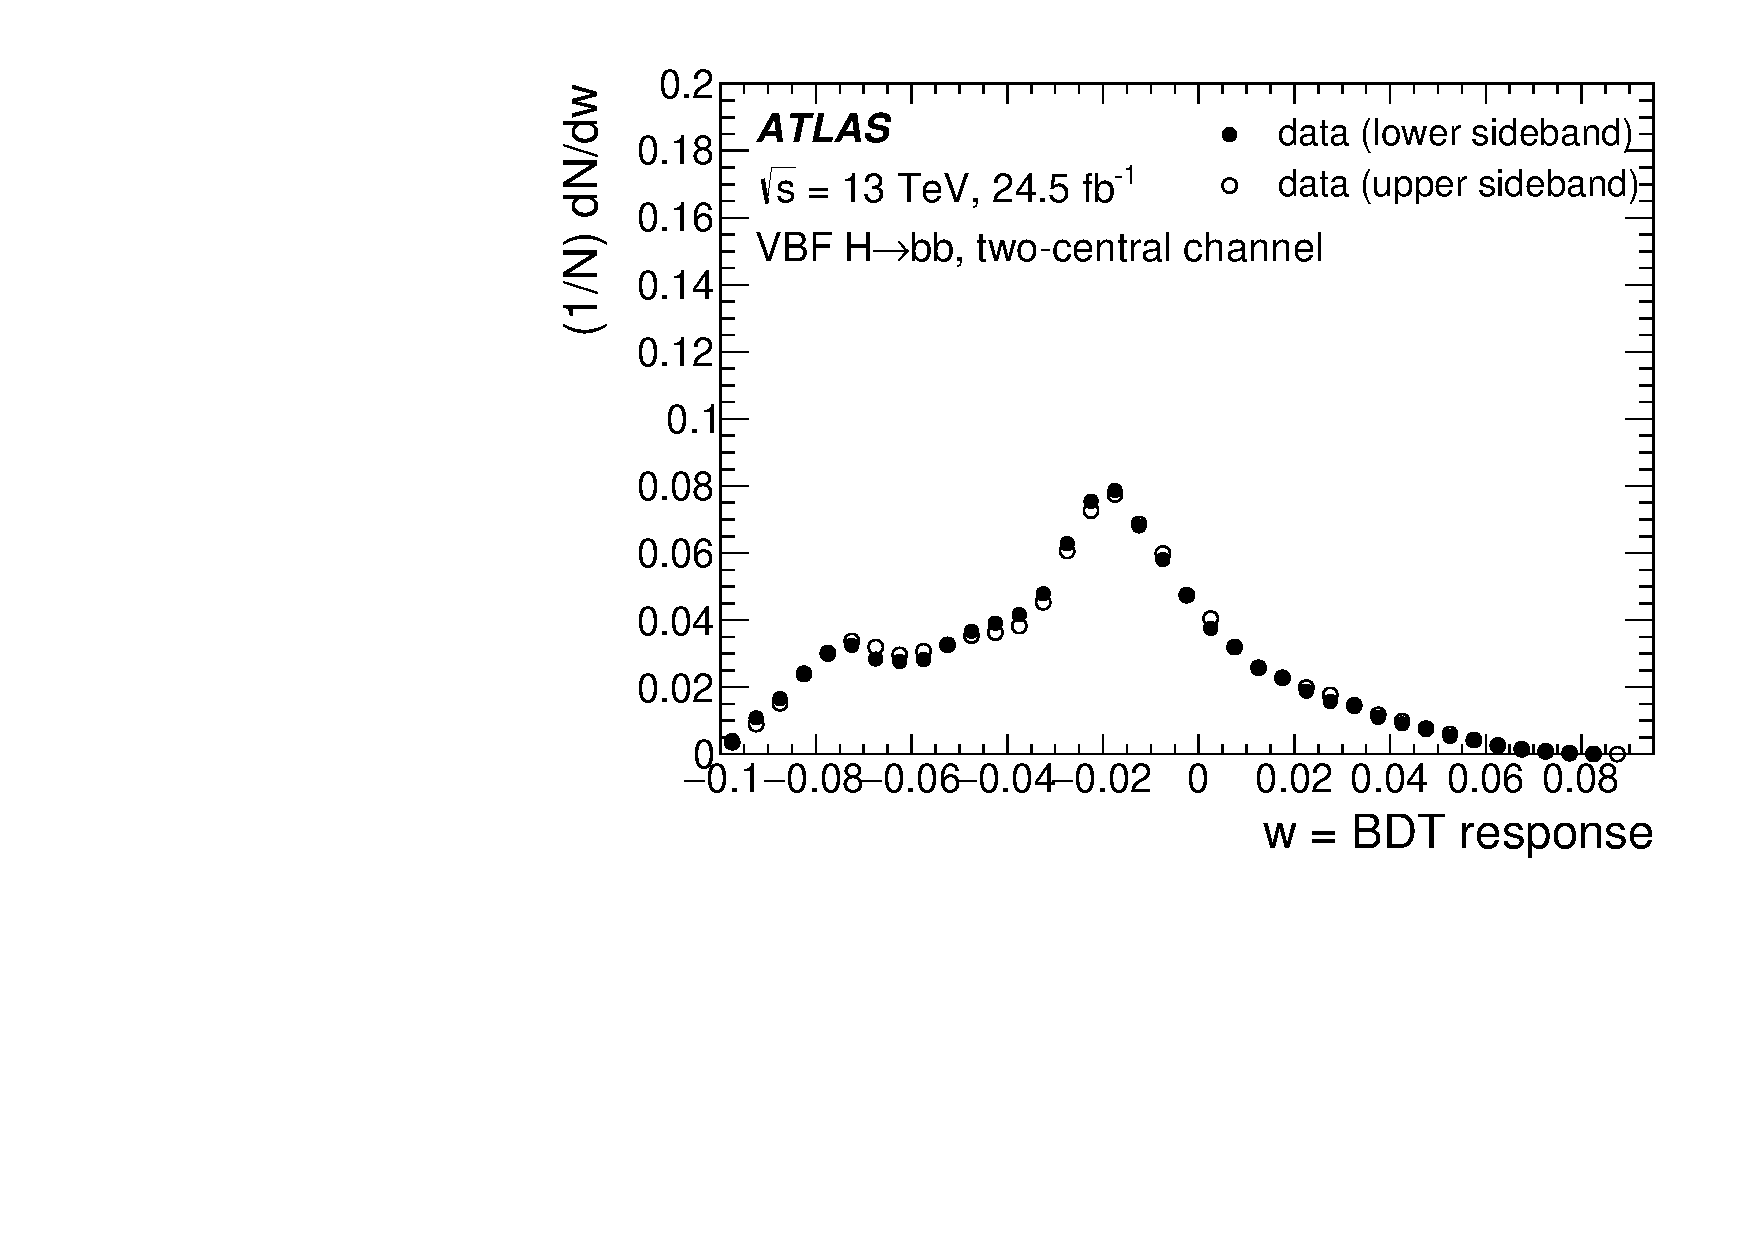
\includegraphics[width=0.48\textwidth]{figures/VBF/VBF_BDT_sidebands_2cen.pdf}
 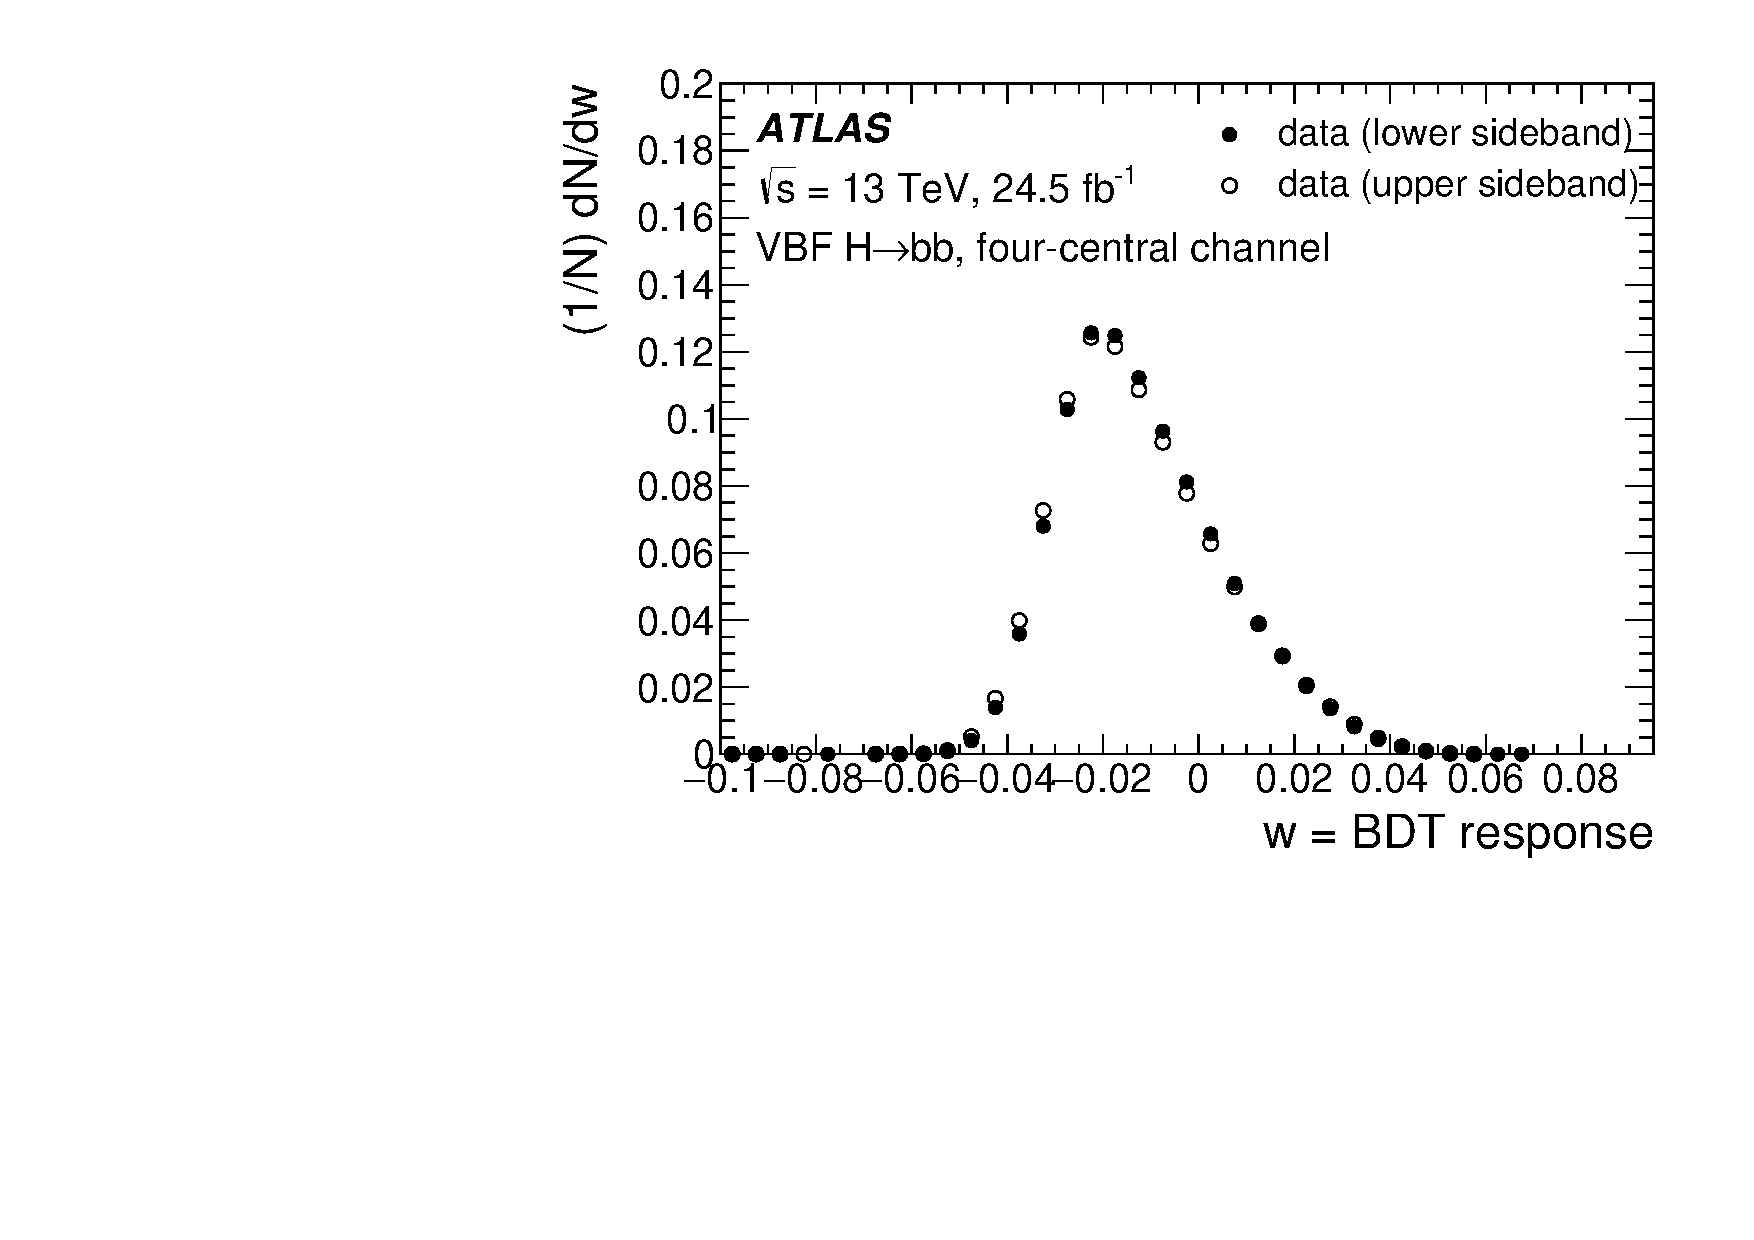
\includegraphics[width=0.48\textwidth]{figures/VBF/VBF_BDT_sidebands_4cen.pdf}
\caption{Comparison of the BDT response distributions between lower and upper data sideband events for the \twocentral (left) and \fourcentral channels. No obvious BDT response dependence on \Mbb is observed. }
  \label{fig:vbf-bdtsidebands}
\end{figure}




%The most correlated variables with \Mbb is $\Delta M_{\rm JJ}$.
%Further studies of the correlation with \Mbb and the BDT variables,
%the relative importance of each variable in the BDT, and a 3-fold
%validation test are shown in Appendix~\ref{sec:vbf-app-bdt}.
%From these studies we conclude that the BDT discriminant is not
%significantly correlated with \Mbb with the exception of very high BDT scores.

The BDT response for  the signal and background training and validation
samples for both channels is shown in Figure~\ref{fig:vbf-BDTResponse}.
In the \fourcentral channel the VBF \Hbb BDT distribution peaks at 0.03.
The background sample peaks at -0.02.  In the \twocentral channel the
VBF \Hbb distribution has a single broad peak at 0.05 and the
background peaks at -0.02. Good agreement is seen between the training
and validation datasets, indicating that the BDT training is adequate.
A Kolmogorov-Smirnov test is used to check the compatibility between
the training and validation datasets.  The \twocentral channel has
a 0.52 $p$-value for the observed agreement in the background sample
and 0.58 $p$-value for the signal sample. The \fourcentral channel has
a $p$-value of 0.95 for the background and $p$-value of 0.99 for the signal.
Figure~\ref{fig:vbf-BDTResponse} also shows the compatibility of the BDT
shapes for all samples considered in this analysis.
The ggF Higgs production and QCD-produced \zjets ~ samples have a
nearly identical response to the background sample in the \fourcentral channel.
In the \twocentral channel these samples have a slightly higher average BDT score than the background distribution.
The EWK \zjets ~ production has a most probable BDT score which is higher than the
background samples, but less than the VBF \Hbb sample in both cases.



\begin{figure}[htbp]
  \centering
 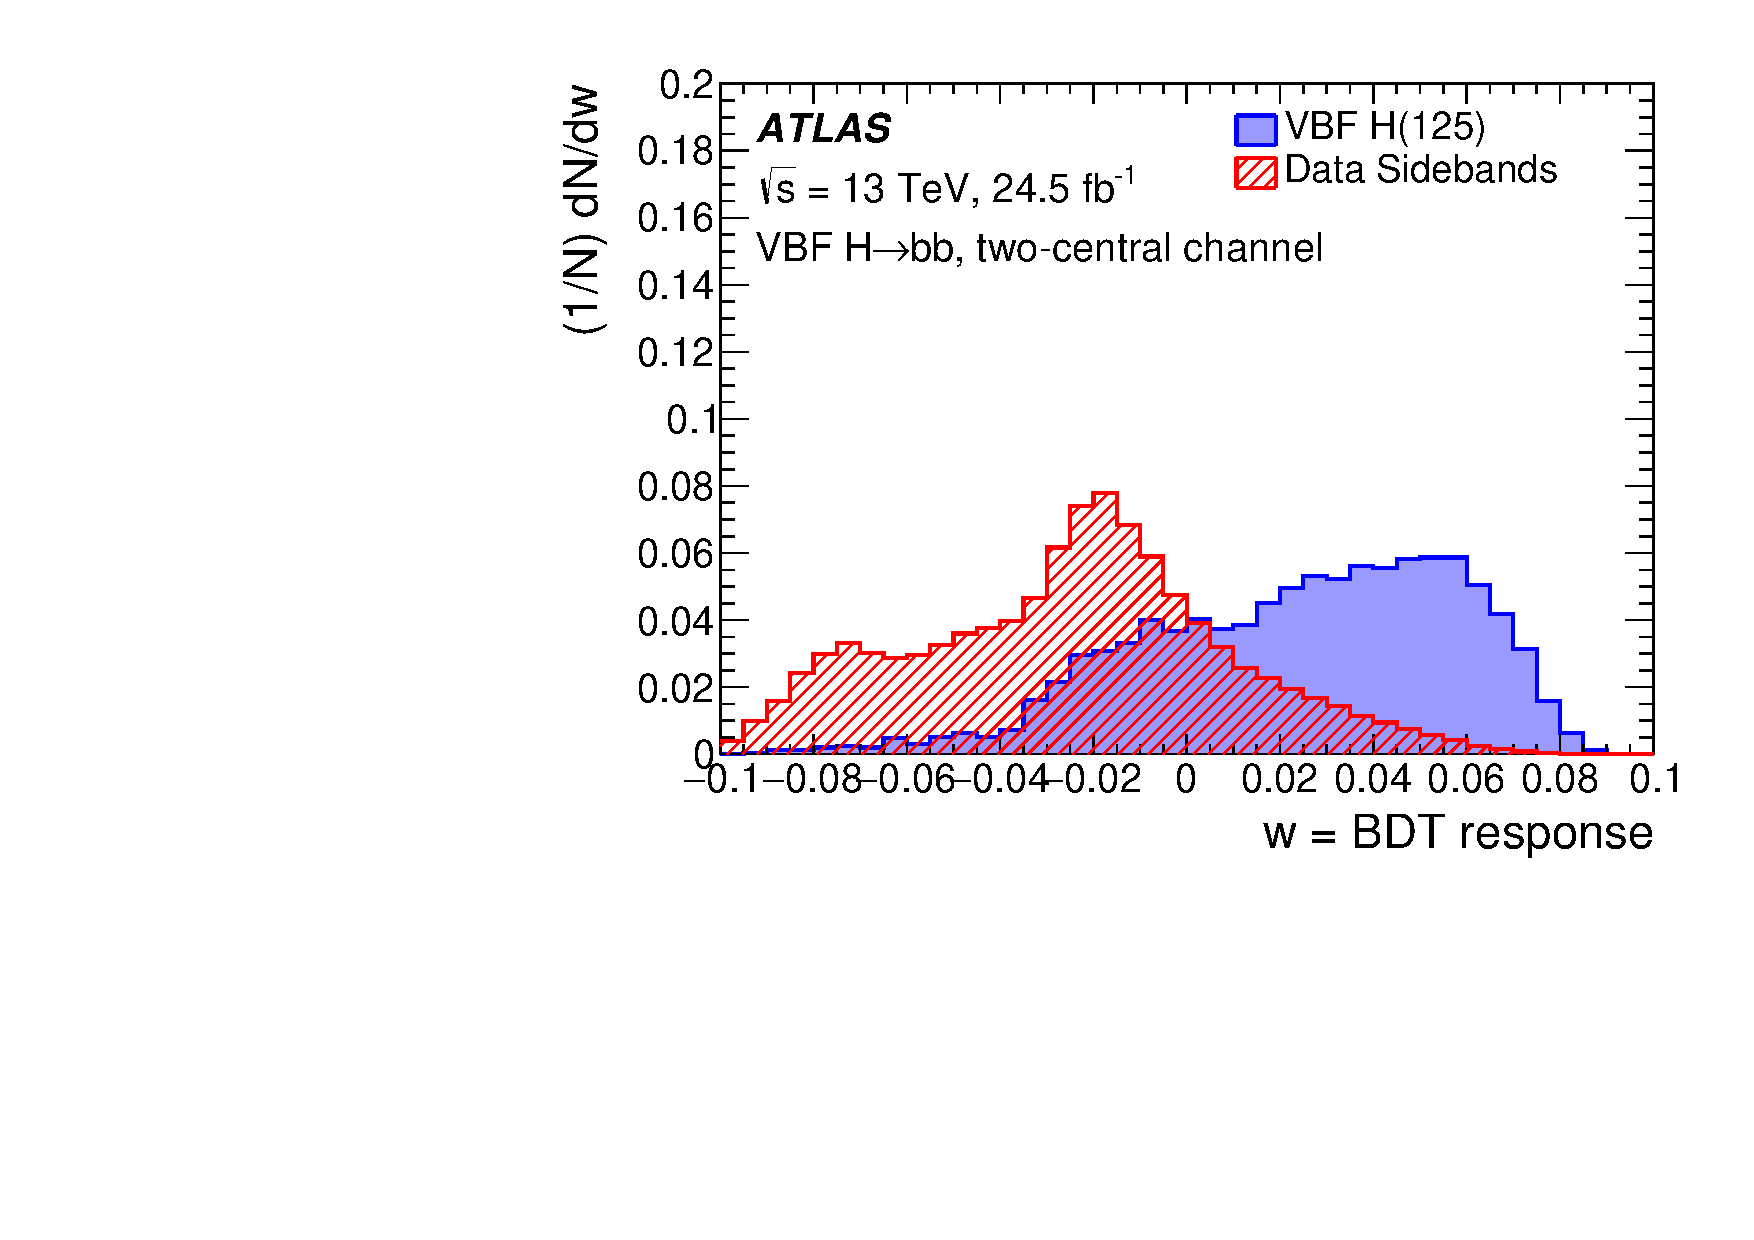
\includegraphics[width=0.48\textwidth]{figures/VBF/BDT_response_2cen.pdf}
 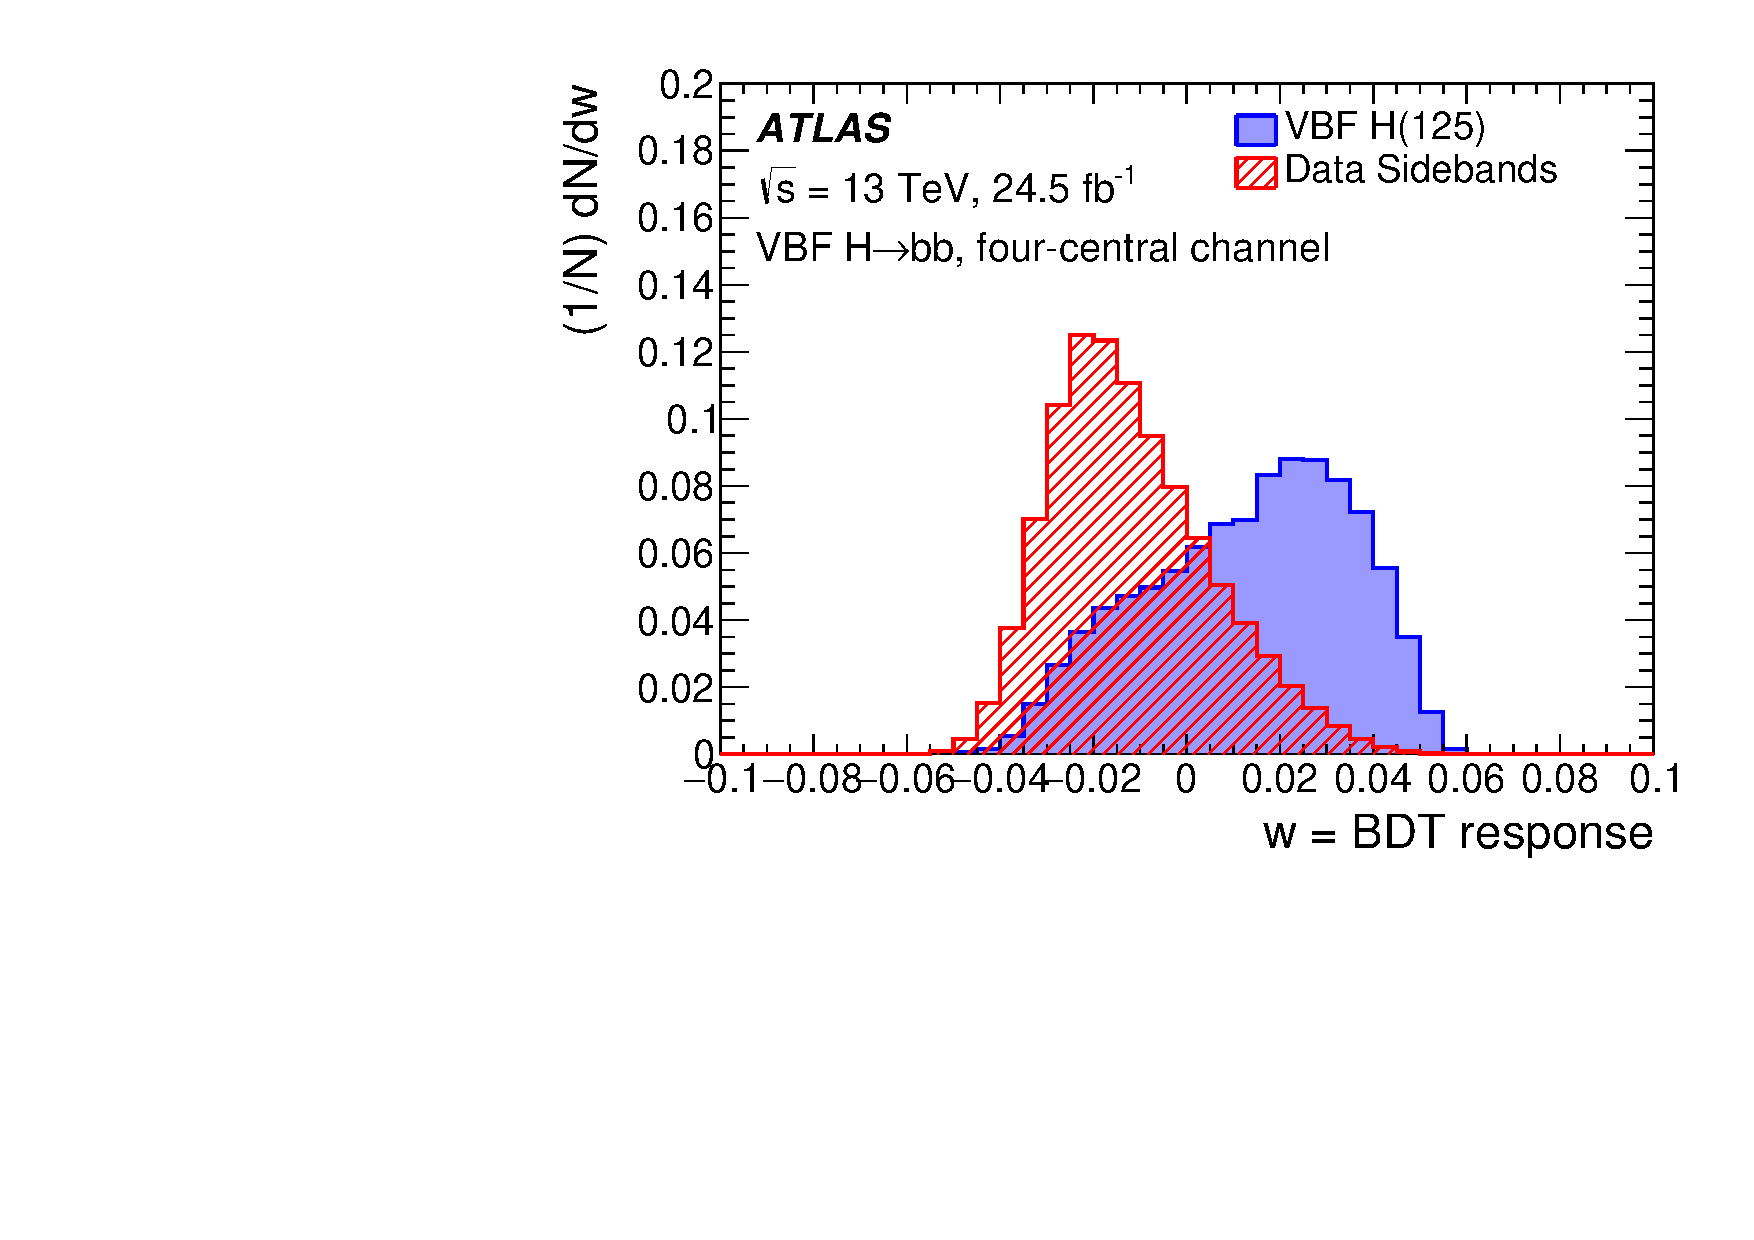
\includegraphics[width=0.48\textwidth]{figures/VBF/BDT_response_4cen.pdf}\\
 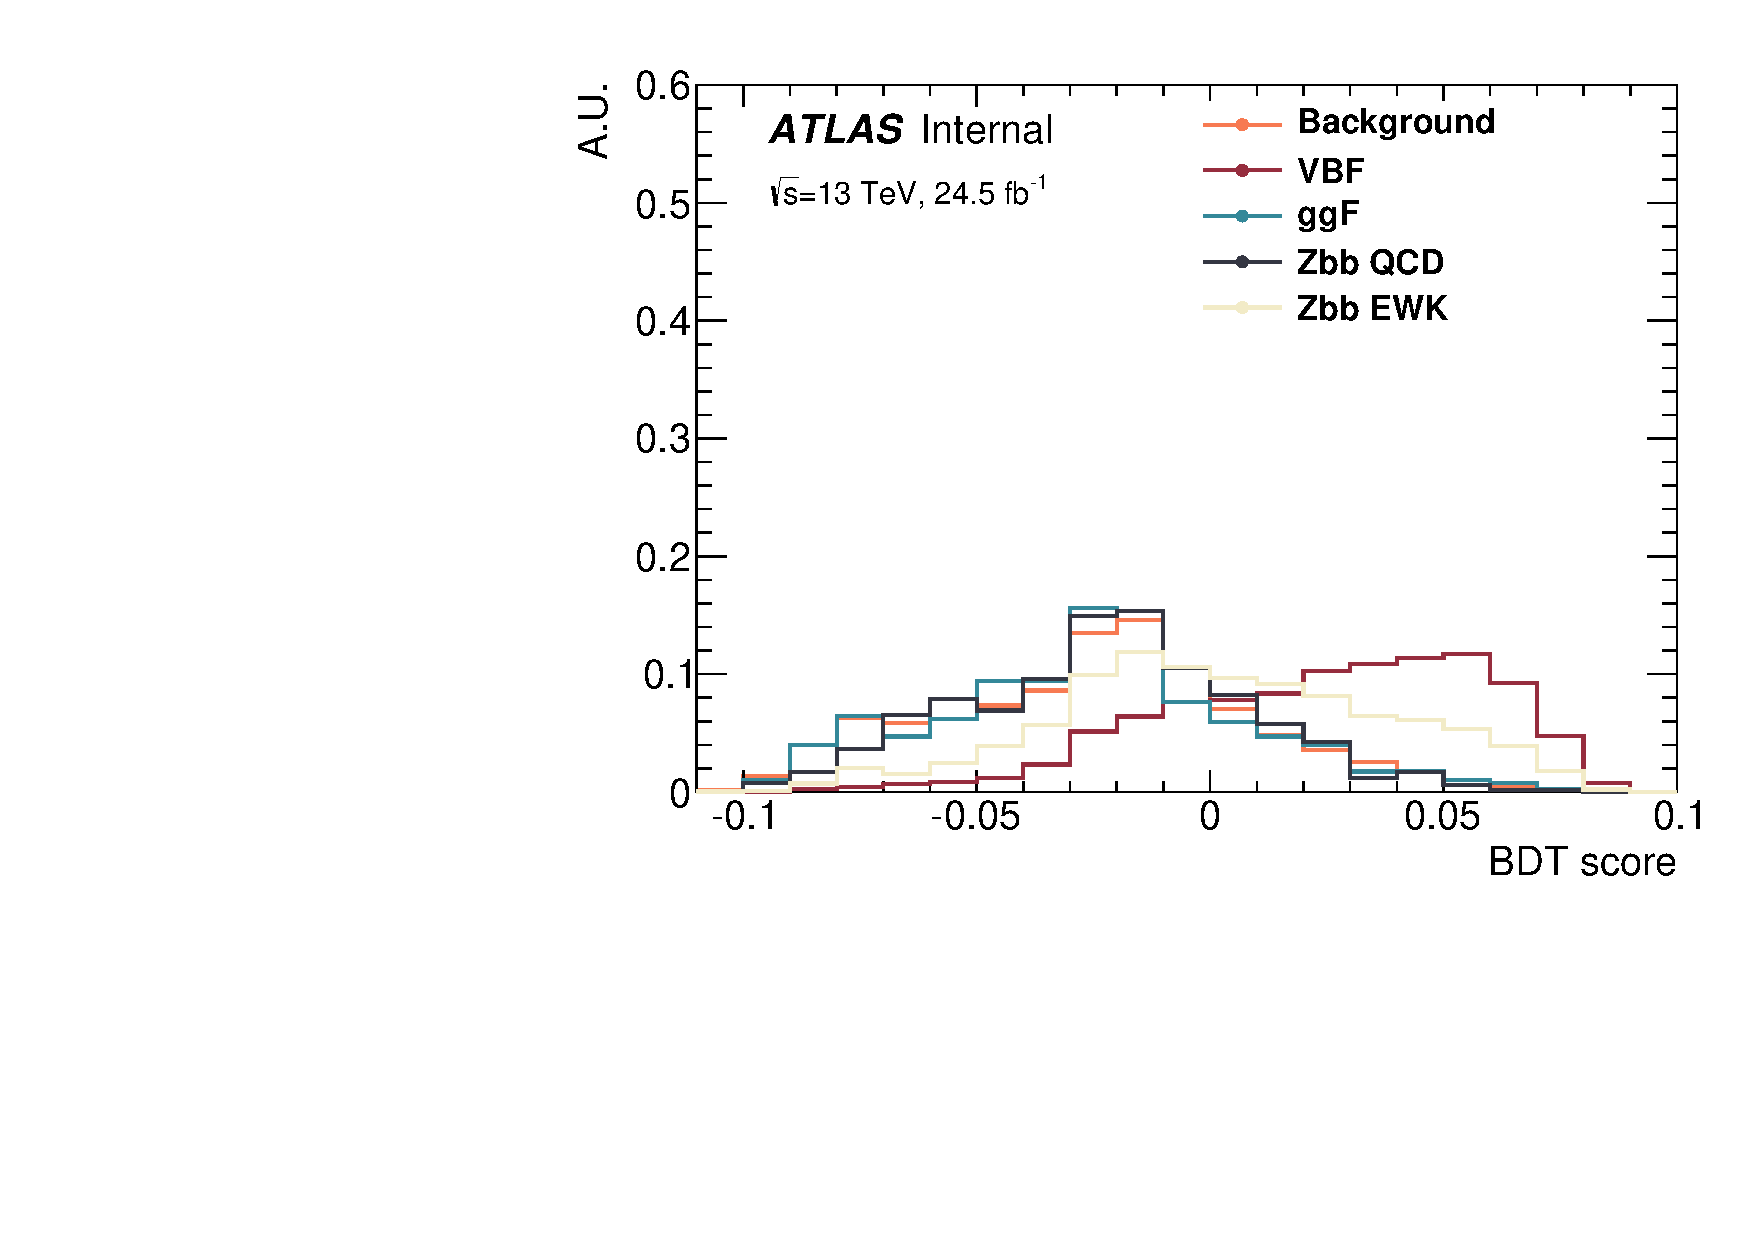
\includegraphics[width=0.48\textwidth]{figures/VBF/BDT_score_breakdown_2cen.pdf}
 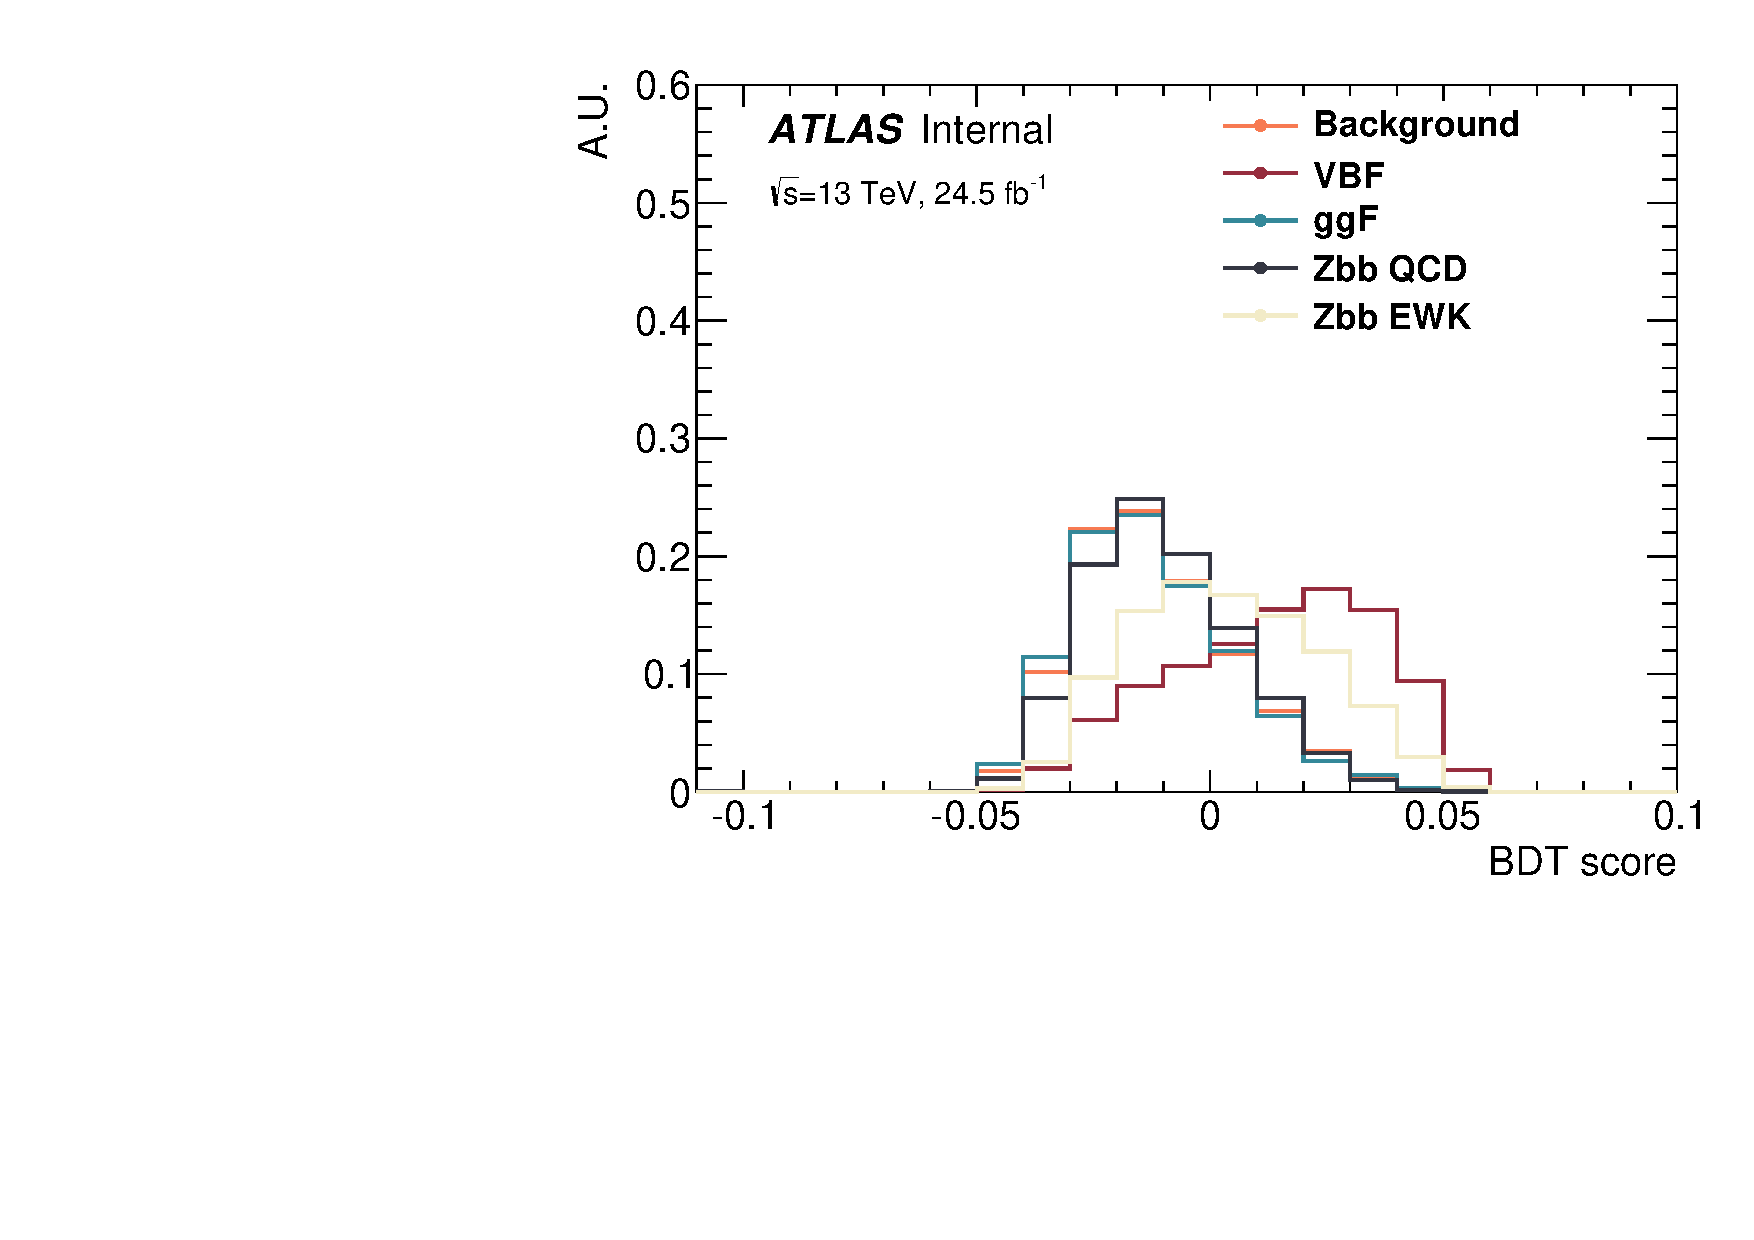
\includegraphics[width=0.48\textwidth]{figures/VBF/BDT_score_breakdown_4cen.pdf}\\
\caption{BDT Response for  the \twocentral (left) and \fourcentral (right) channel.  The top row shows the response for both the training and validation samples.  The bottom row shows a comparison of response for the signal, multijet background, $ggF$ Higgs and $Z$ boson samples. }
  \label{fig:vbf-BDTResponse}
\end{figure}


\subsection{Signal Regions}
For the \twocentral channel, we choose a region in which
a sufficiently large number of \zjets{} events pass the BDT to
adequately control the contribution of this background in the final fit.
The top 80\% of the VBF signal events pass this requirement to define the first signal region.
The second encompasses the remainder of the BDT distribution. This definition of the regions
is a conservative approach that ensures a constraining power of the \zjets{} contribution
sufficient to prevent biasing the Higgs strength as the leading order $Z$ MC
modeling might not be accurate and we have to float its contribution in the fit.

%(see Section~\ref{sec:vbf-ztreat} and Appendix~\ref{sec:vbf-app-alternative2cen} for more details). 
%Alternative definitions of the SRs, aimed at maximizing the sensitivity for the Higgs boson, 
%have been considered and discarded in favor of having higher precision in determining the \zjets{} contribution in each region.
%Table~\ref{tab:BDTSensitivity} illustrates the impact of the choice of SR I definition on the overall Higgs sensitivity and 
%the precision on the \zjets{} contribution in that region.
%For example, extending the lower boundary of the SR I from including 50\% to 80\% VBF events, 
%the \zjets{} contribution grows by a factor of five, corresponding to a 2.7 times improvement in constraining power, while the Higgs sensitivity is reduced by 17\%.   The last column of Table~\ref{tab:BD%TSensitivity} is chosen as the BDT region definition. 

For the \fourcentral channel, we scan the VBF signal events in the entire BDT scores to maximize the sum of $\frac{S}{\sqrt{B}}$ for the top 70\% VBF signal to define in total four signal regions. In this channel, the \zjets{} contribution is larger and the constraining power in each SR is adequate to prevent large bias to the Higgs strength (see Section~\ref{sec:vbf-zunblind}).
Therefore the manual adjustment of the SR boundaries adopted for \twocentral is not necessary.

The definition of the signal regions, the yields of each processes and the estimation of sensitivity are listed in Tables~\ref{tab:BDTReg2cen_alt} and ~\ref{tab:BDTReg4cen_alt}. 


%\begin{table}[]
%\centering
%\caption{Higgs and \zjets{} sensitivity for different definitions of BDT regions in \twocentral channel. The $\Delta \mu_H$ is estimated with Asimov fit for all regions and channels combined. The $\Delta \mu_Z$ is estimated in sideband only fit for SR I of the \twocentral channel. The most sensitive region is always defined to retian VBF events with top x\% BDT scores. The rest of the regions are defined to maximize the sum of $\frac{S}{\sqrt{B}}$. The final configuration we choose is the last column such that we have sufficient constraining power of \zjets{}.}
%\label{tab:BDTSensitivity}
%\resizebox{\textwidth}{!}{
%\begin{tabular}{|c|c|c|c|c|c|}
%\hline
%                                                                                             & \begin{tabular}[c]{@{}c@{}}4 regions\\     SR I top 30\% VBF\end{tabular} & \begin{tabular}[c]{@{}c@{}}3 regions\\   SR I top 50\% VBF\end{tabular} & \begin{tabular}[c]{@{}c@{}}3 regions\\   SR I top 60\% VBF\end{tabular} & \begin{tabular}[c]{@{}c@{}}3 regions\\   SR I top 70\% VBF\end{tabular} & \begin{tabular}[c]{@{}c@{}}2 regions\\   SR I top 80\% VBF\end{tabular} \\ \hline
%$\Delta \mu_H$                                                                               & 1.4                                                                       & 1.67                                                                    & 1.71                                                                    & 1.78                                                                    & 1.84                                                                    \\ \hline
%\begin{tabular}[c]{@{}c@{}}$\Delta \mu_Z$\\ 2 central SR I\\ Sideband only fit\end{tabular}  & 5.0                                                                       & 3.37                                                                    & 2.6                                                                     & 1.6                                                                     & 1.25                                                                    \\ \hline
%\begin{tabular}[c]{@{}c@{}}\# Z events in \\ the side band of \\ 2 central SR I\end{tabular} & 51.19                                                                     & 140.8                                                                   & 214.5                                                                   & 445.3                                                                   & 760.34                                                                  \\ \hline
%\begin{tabular}[c]{@{}c@{}}\# Z events in\\  the sideband of \\ the rest of SRs\end{tabular} & 2263.7                                                                    & 2574.1                                                                  & 2500.4                                                                  & 2269.6                                                                  & 1954.56                                                                 \\ \hline
%\end{tabular}}
%\end{table}


\begin{table}[htpb]
\centering
\begin{tabular}{|l|l|l|}
\hline
Region                       & SR I                  & SR II                 \\ \hline
BDT Score Range              & \textgreater -0.006    & \textless -0.006       \\ \hline
\multicolumn{3}{|c|}{Total Yield}                                            \\ \hline
QCD $Z$                      & $946.2 \pm 91.1$    & $2525.3 \pm 145.9$  \\ \hline
EWK $Z$                      & $70.9 \pm 2.3$      & $54.6 \pm 2.1$      \\ \hline
\multicolumn{3}{|c|}{Sideband}                                               \\ \hline
Non-resonant (sideband low)  & $22812 \pm 151.0$    & $62742 \pm 250.5 $   \\ \hline
Non-resonant (sideband high) & $38020 \pm 195.2$    & $100936 \pm 317.7 $  \\ \hline
\multicolumn{3}{|c|}{Yield in Higgs Mass Window}                             \\ \hline
VBF                          & $101.2 \pm 2.0$     & $22.2\pm 0.9$       \\ \hline
ggF                          & $23.7 \pm 2.6$      & $75.8\pm 6.1$       \\ \hline
Non-resonant (extrapolated)   & $32546.0 \pm 180.4$ & $92738.2 \pm 304.5$ \\ \hline
\multicolumn{3}{|c|}{Expected Sensitivity}                                   \\ \hline
$S/ \sqrt(B)$                & 0.70                  & 0.32                  \\ \hline
\end{tabular}
\caption{Signal region definitions, yields and sensitivities for the \twocentral channel. }
\label{tab:BDTReg2cen_alt}

\end{table}


\begin{table}[htpb]
\centering
\begin{tabular}{|l|l|l|l|l|}
\hline
Region                       & SR I                & SR II                      & SR III                     & SR IV                      \\ \hline
BDT Score Range              & \textgreater0.033   & [0.026, 0.033]             & [0.015, 0.026]             & [0.002, 0.015]             \\ \hline
\multicolumn{5}{|c|}{Total Yield}                                                                                                         \\ \hline
QCD $Z$                      & $64.1 \pm 14.8$   & $787.8 \pm 66.2$         & $2485.9 \pm 132.1$       & $7274.4 \pm 206.1$       \\ \cline{2-5} 
EWK $Z$                      & $12.3 \pm 0.8$    & $63.5 \pm 1.7$           & $128.2 \pm 2.4$          & $184.0 \pm 2.9$          \\ \hline
\multicolumn{5}{|c|}{Sideband}                                                                                                            \\ \hline
Non-res. (sideband low)  & $8626 \pm 92.9$    & $13998 \pm 118.3 $        & $43393 \pm 208.3$         & $108343 \pm 329.2$        \\ \cline{2-5} 
Non-res. (sideband high) & $12267 \pm 110.8$  & $18550 \pm 136.2$         & $55413 \pm 235.4$         & $134435 \pm 366.7$        \\ \hline
\multicolumn{5}{|c|}{Yield in Higgs Mass Window}                                                                                          \\ \hline
VBF                          & $51.6 \pm 0.6$    & $28.4\pm 0.3$            & $43.1\pm 0.5$            & $41.9\pm 0.5$            \\ \cline{2-5} 
ggF                          & $11.3 \pm 0.4$    & $13.2 \pm 0.4$           & $43.4 \pm 1.4$           & $127.0 \pm 1.5$          \\ \cline{2-5} 
Non-res. (extrapolated)   & $8797.1 \pm 93.8$ & $15685.8\pm 125.2$       & $53156.7\pm 230.6$       & $142273.1\pm 377.2$      \\ \hline
\multicolumn{5}{|c|}{Expected Sensitivity}                                                                                                \\ \hline
$S/ \sqrt(B)$                & 0.67                & 0.33                       & 0.38                       & 0.45                       \\ \hline
\end{tabular}
\caption{Signal region definitions, yields and sensitivities for the \fourcentral channel. }
\label{tab:BDTReg4cen_alt}

\end{table}



\clearpage

\section{Statistical Analysis}
This section describes the signal extraction strategy. In order to describe the data, we consider three contributions to the \Mbb{} distribution:  
\begin{itemize}
  \item Signal \Hbb from either VBF or ggF production
  \item Resonant \zjets{} from QCD and EW production
  \item Non-resonant processes dominated by QCD multi-jet production
\end{itemize}

The shapes of the signal and \zjets{} contributions are each parameterized by a Bukin function as described in \ref{sec:vbf-parsigz}. The non-resonant background is taken from data using a fit with an analytical function in the \Mbb{} sidebands of the signal regions and control region as described in Section~\ref{sec:vbf-nonres}.
The signal strength is measured with a profile likelihood fit performed simultaneously for all signal and control regions.

It is noteworthy that the $Z$ normalization is treated as a nuisance parameter in the fit. The \zjets{} contribution plays an important role in the overall fitting procedure due to the fact that it comprises a significant fraction lower \Mbb{} sideband ( 1--7 (2--4)\% of the \fourcentral(\twocentral) selection), yet the sideband does not extend to low enough \Mbb{} values to reliably constrain its contribution using the shape templates.  Therefore, the non-resonant background fit can be partially compensated by the $Z$-yield and vice-versa.  To mitigate the impact of this degeneracy, we could fix the contributions of \zjets{} in the fits to predictions from MC.  However, our \zjets{} MC is only leading order ($Z+$2 partons), and large or varying $k$-factors may be present in the different BDT regions.  Therefore, we assume no prior knowledge of $Z$ contribution in all BDT regions and allow the contribution to float in the profile likelihood fit. This is the most conservative strategy and yields the largest decrease in overall sensitivity.

To validate the fit closure and conduct sensitivity study, Asimov datasets are constructed. An Asimov dataset is the sum of the Higgs signal, \zjets{} process and the analytical non-resonant background. The parameterization of Higgs signal and \zjets{} components are described in \ref{sec:vbf-parsigz}. The normalization of the Higgs signal and \zjets{} components is the product of the expected strength and the yield taken from MC prediction. The parameterization of the analytical non-resonant background is described in \ref{sec:vbf-nonres}.

%The normalization of the non-resonant background is estimated by scaling the number of events of the 0-tag sample by the ratio of the events in the sidebands for the 2- and 0-tag samples. Specifically $B$ is given by $N_{\rm 0~tag, mw}\times \frac{N_{\rm 2~tag, sb}}{N_{\rm 0~tag, sb}}$ where  $N_{\rm 0~tag, mw}$ is the number of events from the 0-tag sample in the Higgs mass window, and $N_{\rm 2(0)~tag, sb}$ is the number of events in the side-band regions for 2(0)-tag sample.

%\subsection{Treatment of \zjets{} contribution}
%\label{sec:vbf-ztreat}

\subsection{Signal and \zjets Parameterization}
\label{sec:vbf-parsigz}

We parameterize the signal and \zjets{} Monte Carlo templates to smooth out the local fluctuations coming from the limited statistics using a histogrammed Bukin function. The MC templates and parametrization of signal and \zjets{} \Mbb{} distributions are shown in Figures~\ref{fig:vbf-sigpar_alt} and \ref{fig:vbf-zpar_alt}. The $\chi^2$ between simulated and fitted distributions are summarized in Table~\ref{tab:sigpar_alt}. In general, the $\Mbb$ distributions for the Higgs signal and \zjets{} are well represented by the Bukin function. The potential bias of using smoothed MC templates is studied in the full profile likelihood fit. Perfect closure is obtained with $\mu_{H}=1$ and $\mu_{Z}=1$, as injected in the Asimov data.  Therefore we conclude that the parameterized templates produce no significant bias.  The likelihood fit is described in detail later in this section.

\begin{table}[htbp]
\centering
\begin{tabular}{|c|c|c|c|c|}
\hline
\multicolumn{5}{|c|}{$H\rightarrow b\bar b$ \fourcentral}                                                    \\ \hline
Region                                & \multicolumn{2}{c|}{SR I}        & \multicolumn{2}{c|}{SR II}        \\ \hline
\multicolumn{1}{|l|}{$\chi^2$ (Prob)} & \multicolumn{2}{c|}{0.85(0.64)}  & \multicolumn{2}{c|}{1.01(0.44)}   \\ \hline
\multicolumn{5}{|c|}{$H\rightarrow b\bar b$ \twocentral}                                                   \\ \hline
Region                                & SR I            & SR II          & SR III           & SR IV          \\ \hline
\multicolumn{1}{|l|}{$\chi^2$ (Prob)} & 1.06 (0.39)     & 0.77 (0.71)    & 1.10 (0.35)      & 1.21 (0.25)    \\ \hline
\multicolumn{5}{|c|}{\zjets}                                                                                 \\ \hline
Channel                               & \multicolumn{2}{c|}{\twocentral} & \multicolumn{2}{c|}{\fourcentral} \\ \hline
\multicolumn{1}{|l|}{$\chi^2$ (Prob)} & \multicolumn{2}{c|}{1.7 (0.04)}  & \multicolumn{2}{c|}{1.32 (0.17)}  \\ \hline
\end{tabular}
\caption{Goodness of fit for the Bukin parameterizations and signal and \zjets{} \Mbb{} distributions. There are not enough events for the \zjets{} sample to divide amongst BDT regions, therefore a the goodness of fit is shown for each channel preselection.}
\label{tab:sigpar_alt}
\end{table}

\begin{figure}[htbp]
  \centering    
 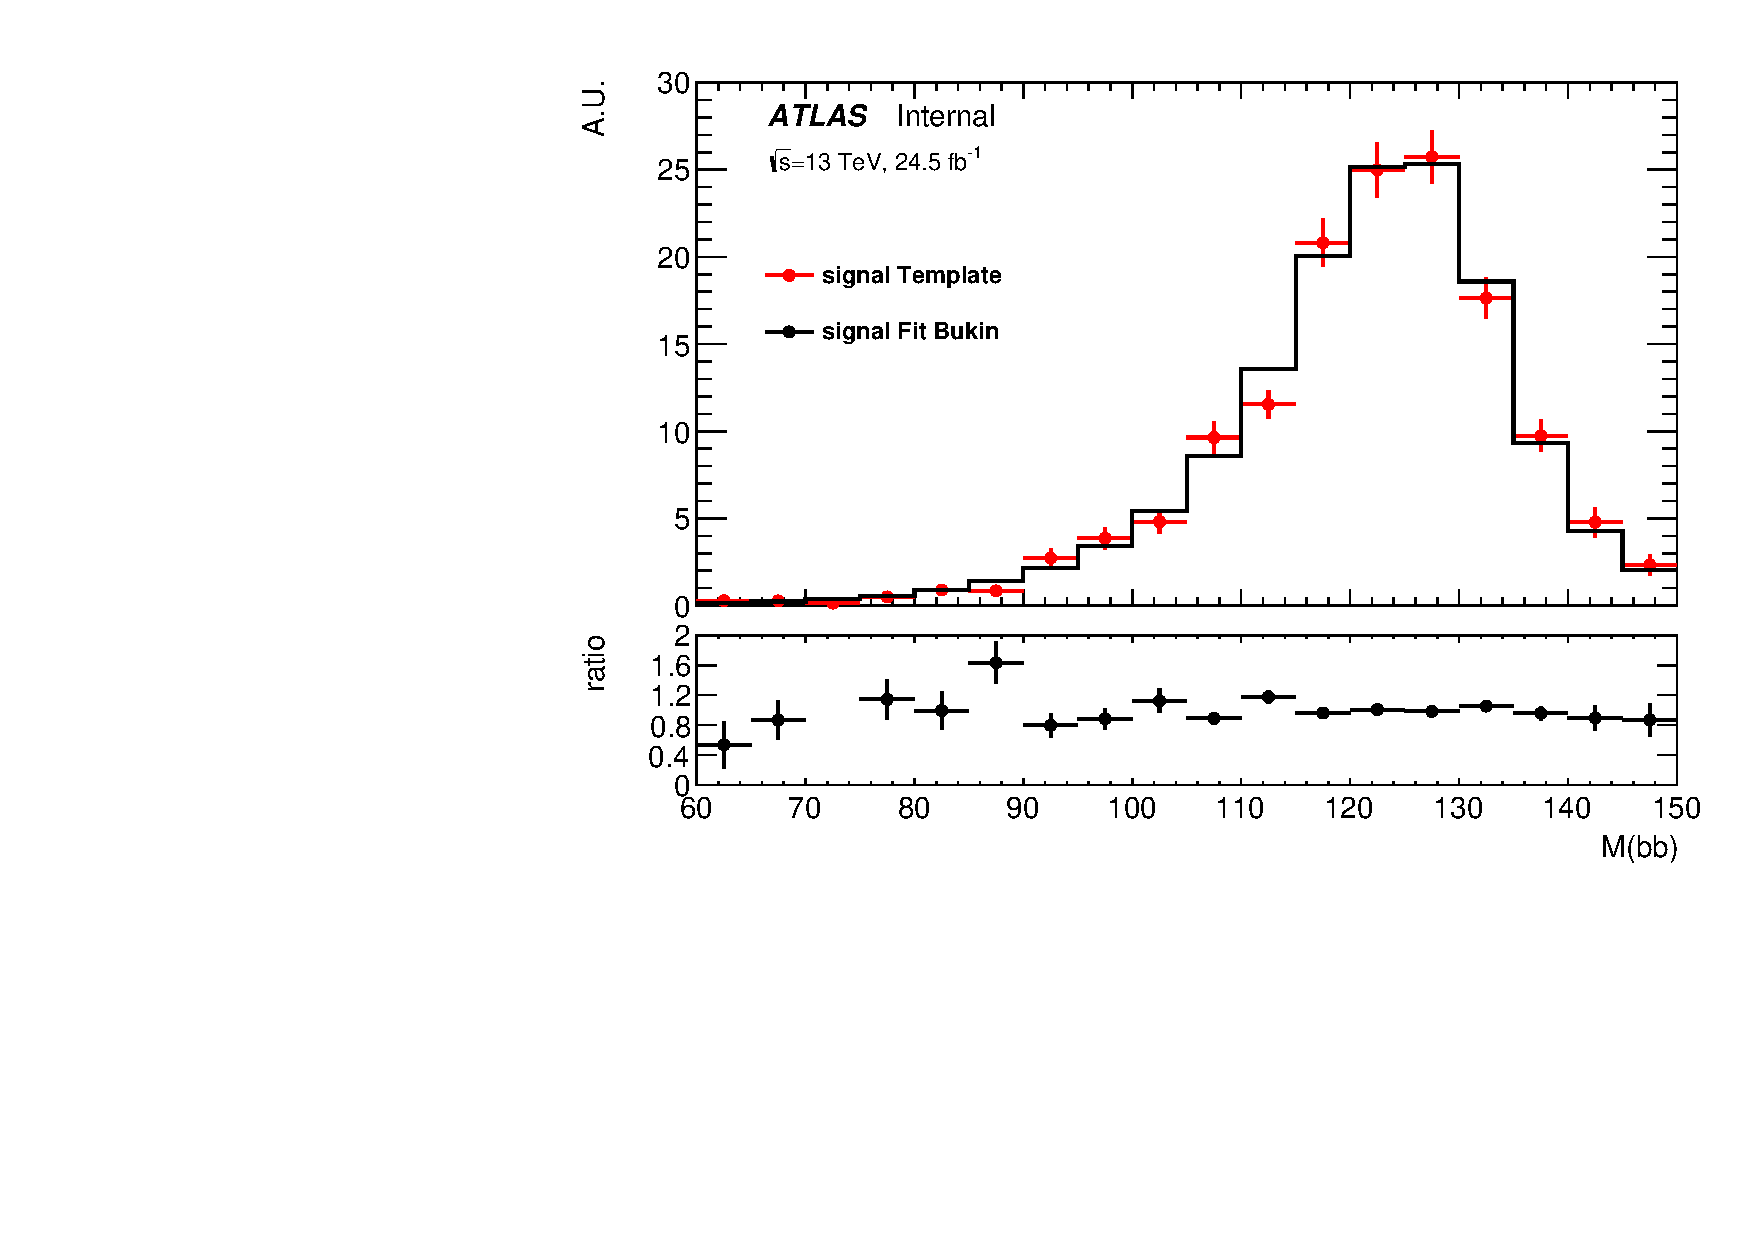
\includegraphics[width=0.45\textwidth]{figures/VBF/sig_2cen_SRI.pdf}
% 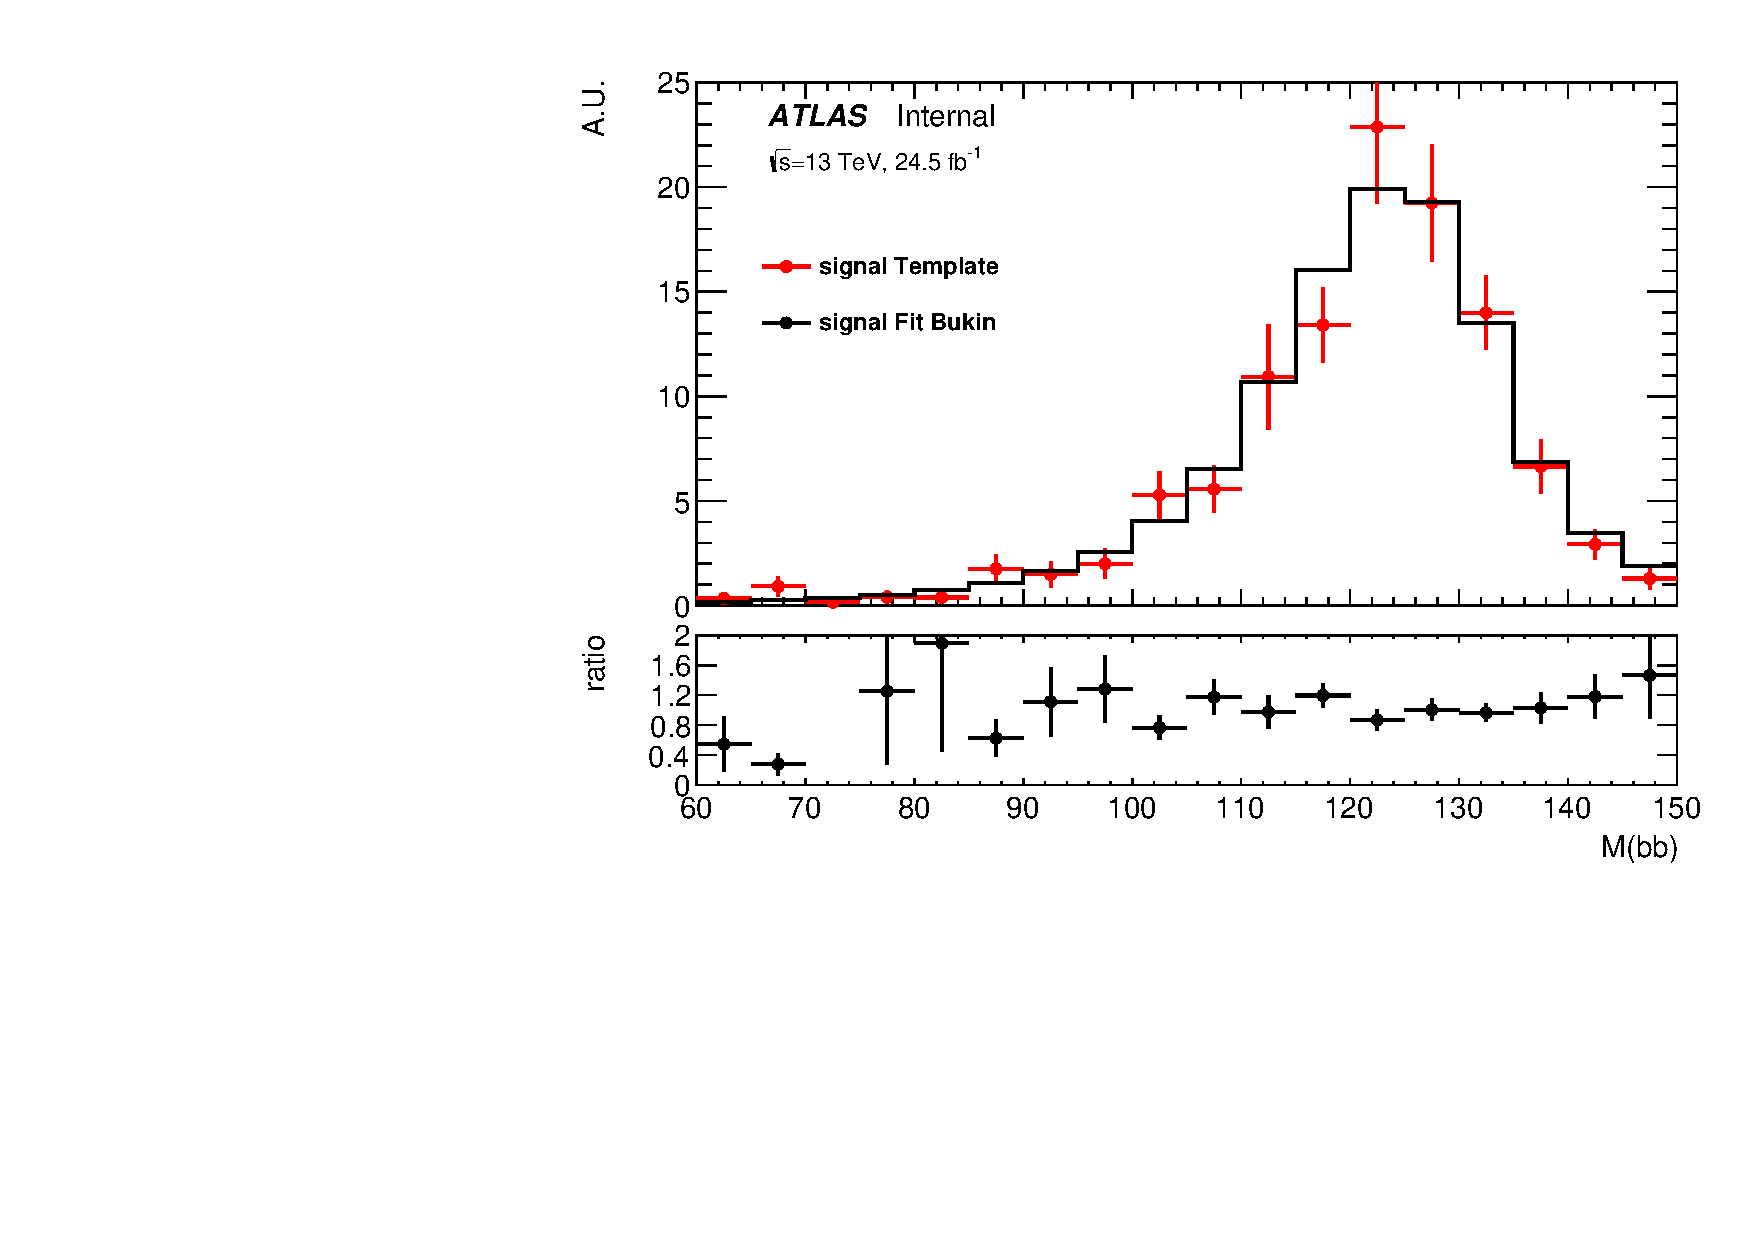
\includegraphics[width=0.24\textwidth]{figures/VBF/sig_2cen_SRII.pdf}\\
 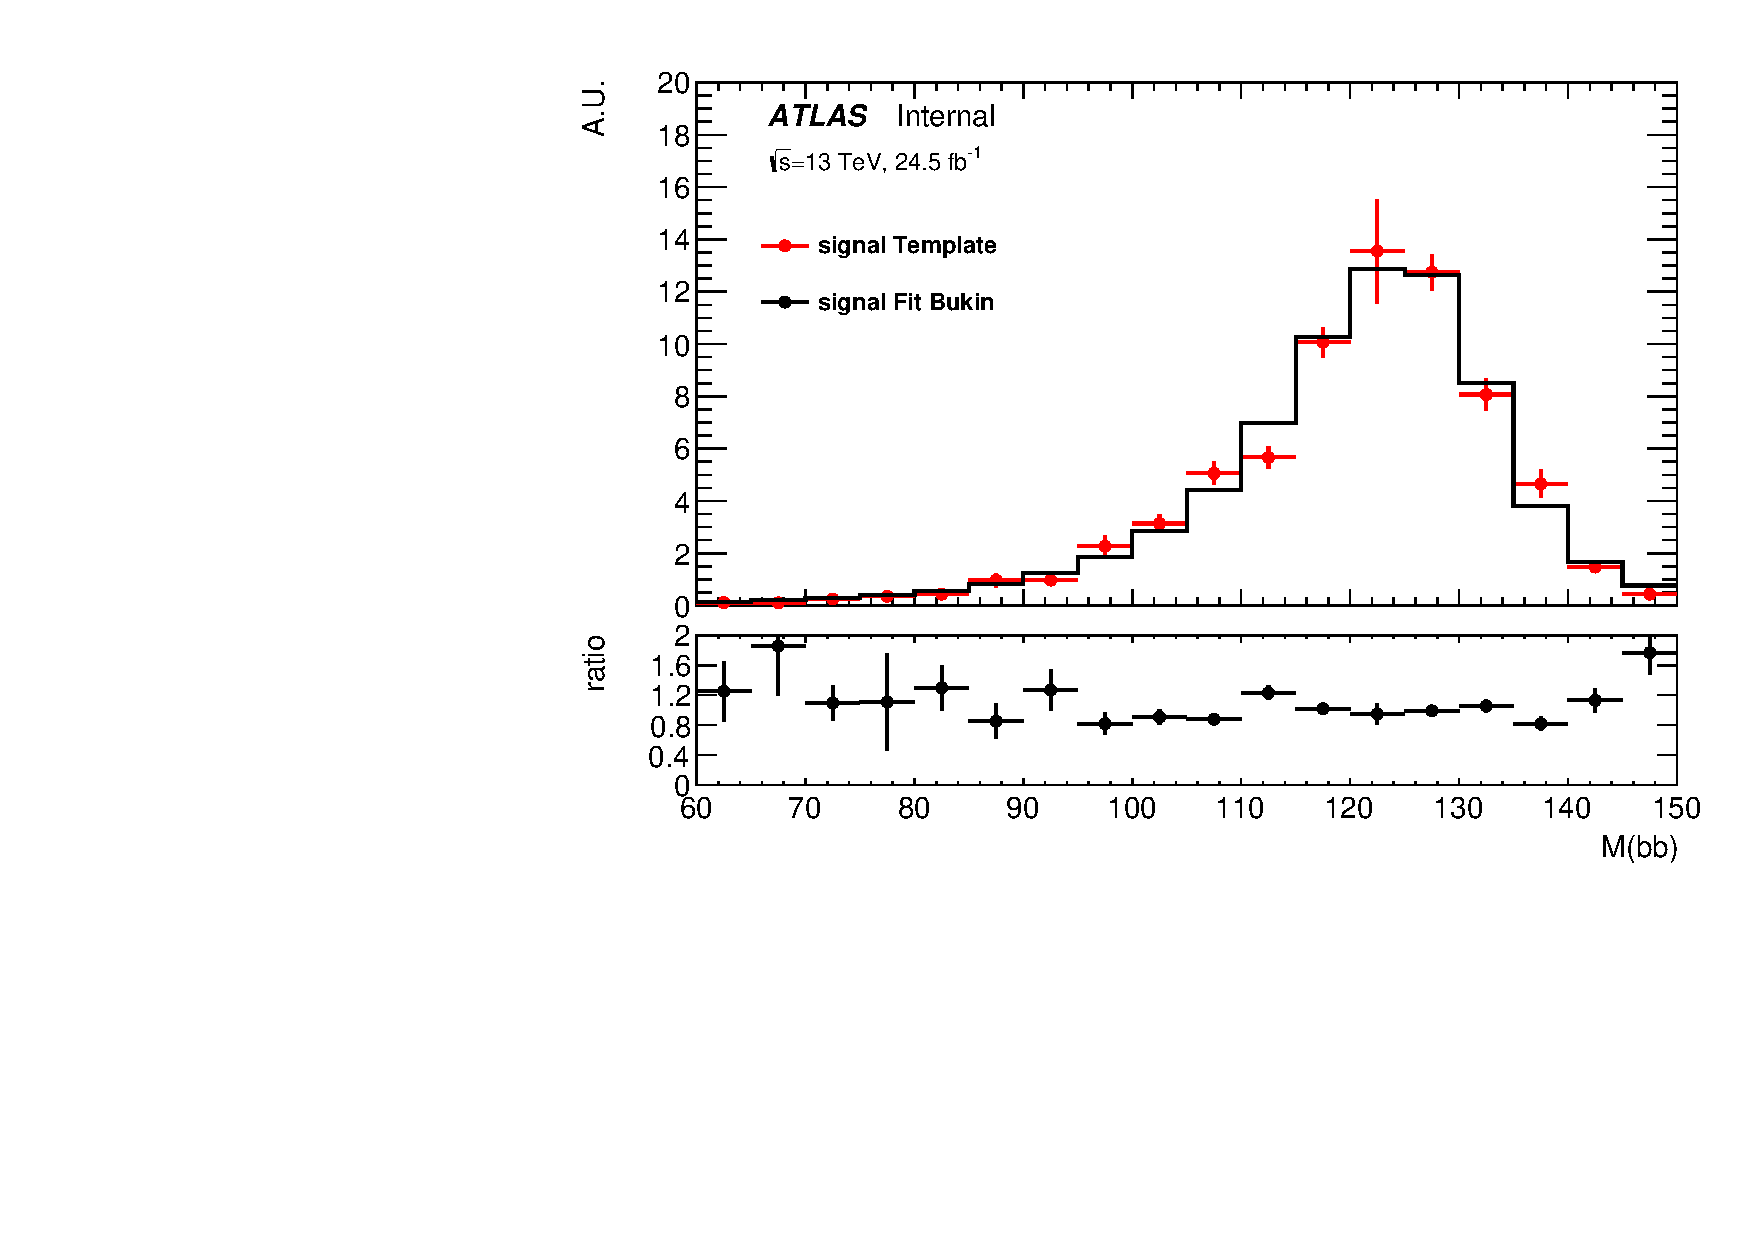
\includegraphics[width=0.45\textwidth]{figures/VBF/sig_4cen_SRI.pdf}
% 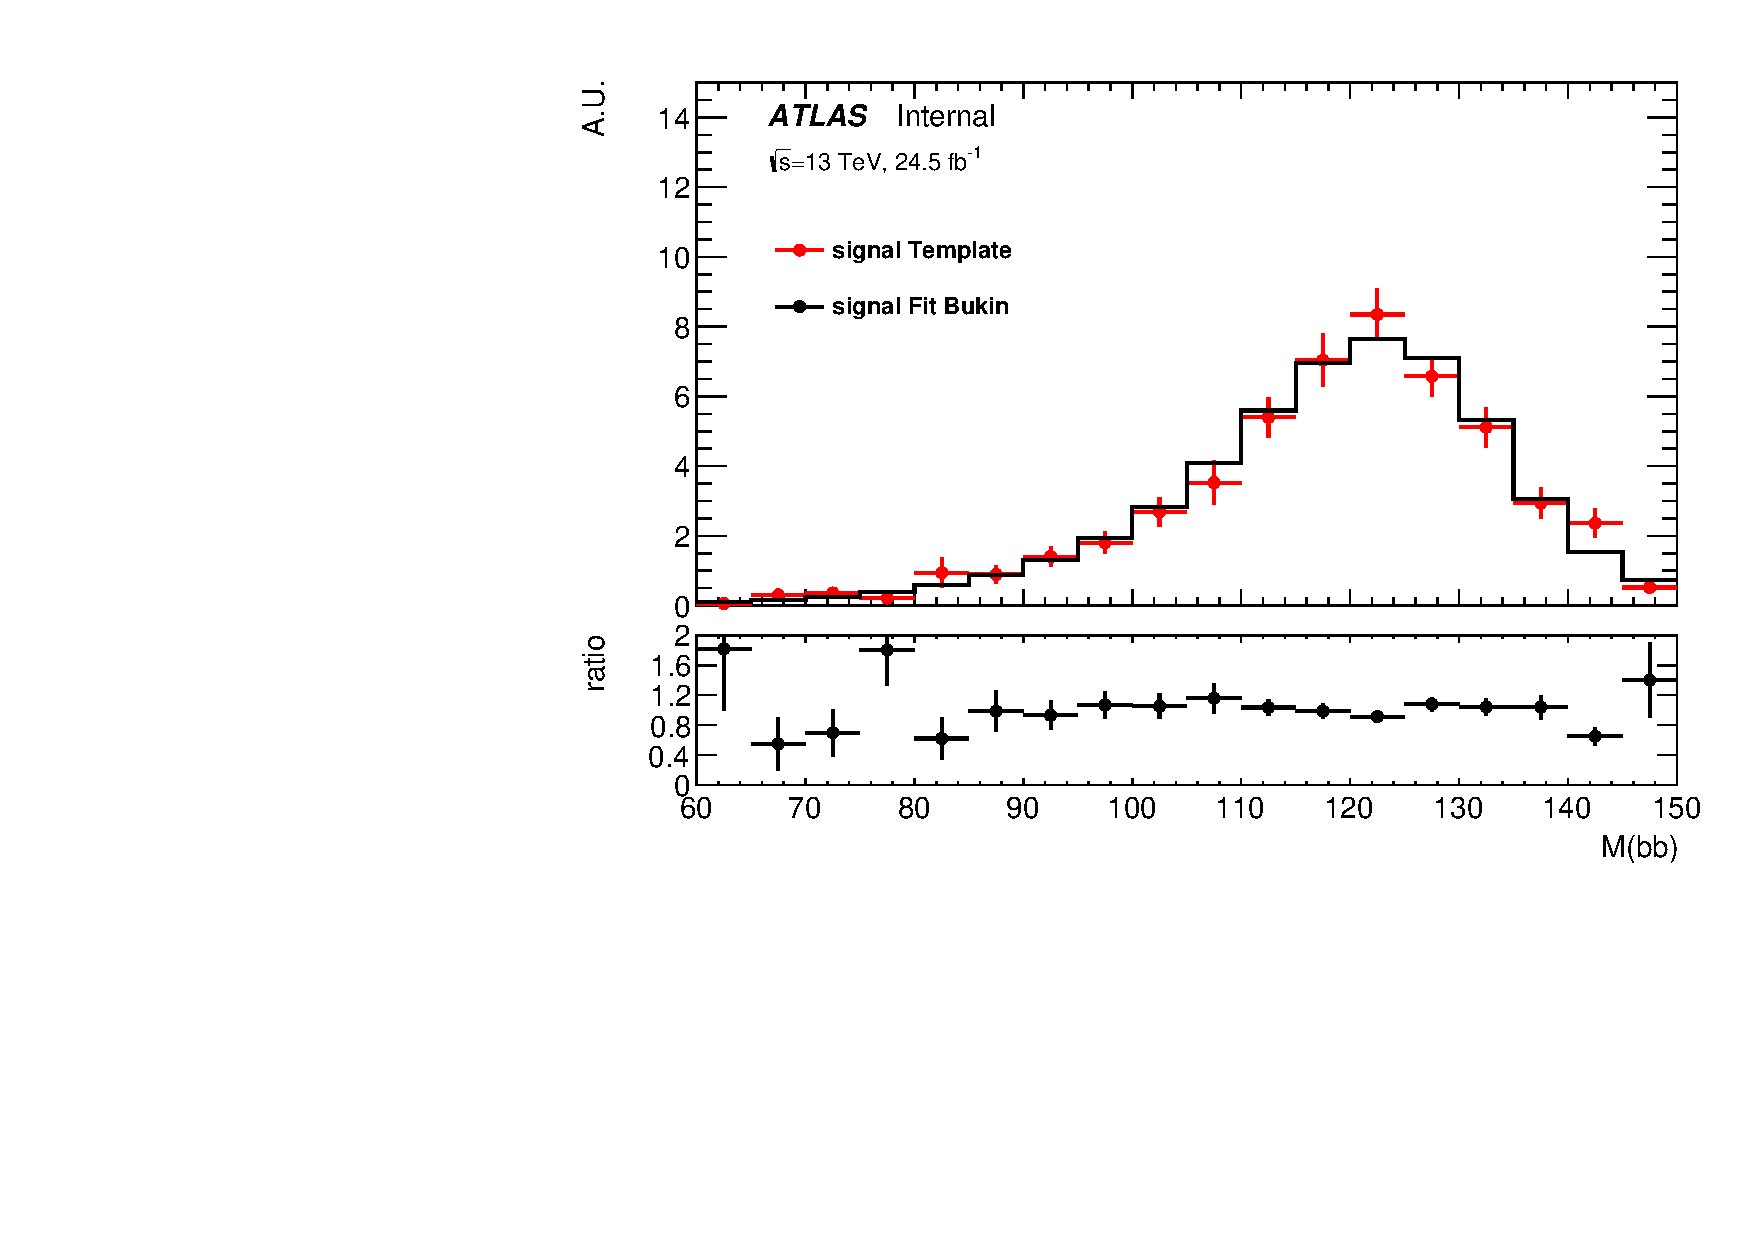
\includegraphics[width=0.24\textwidth]{figures/VBF/sig_4cen_SRII.pdf}
% 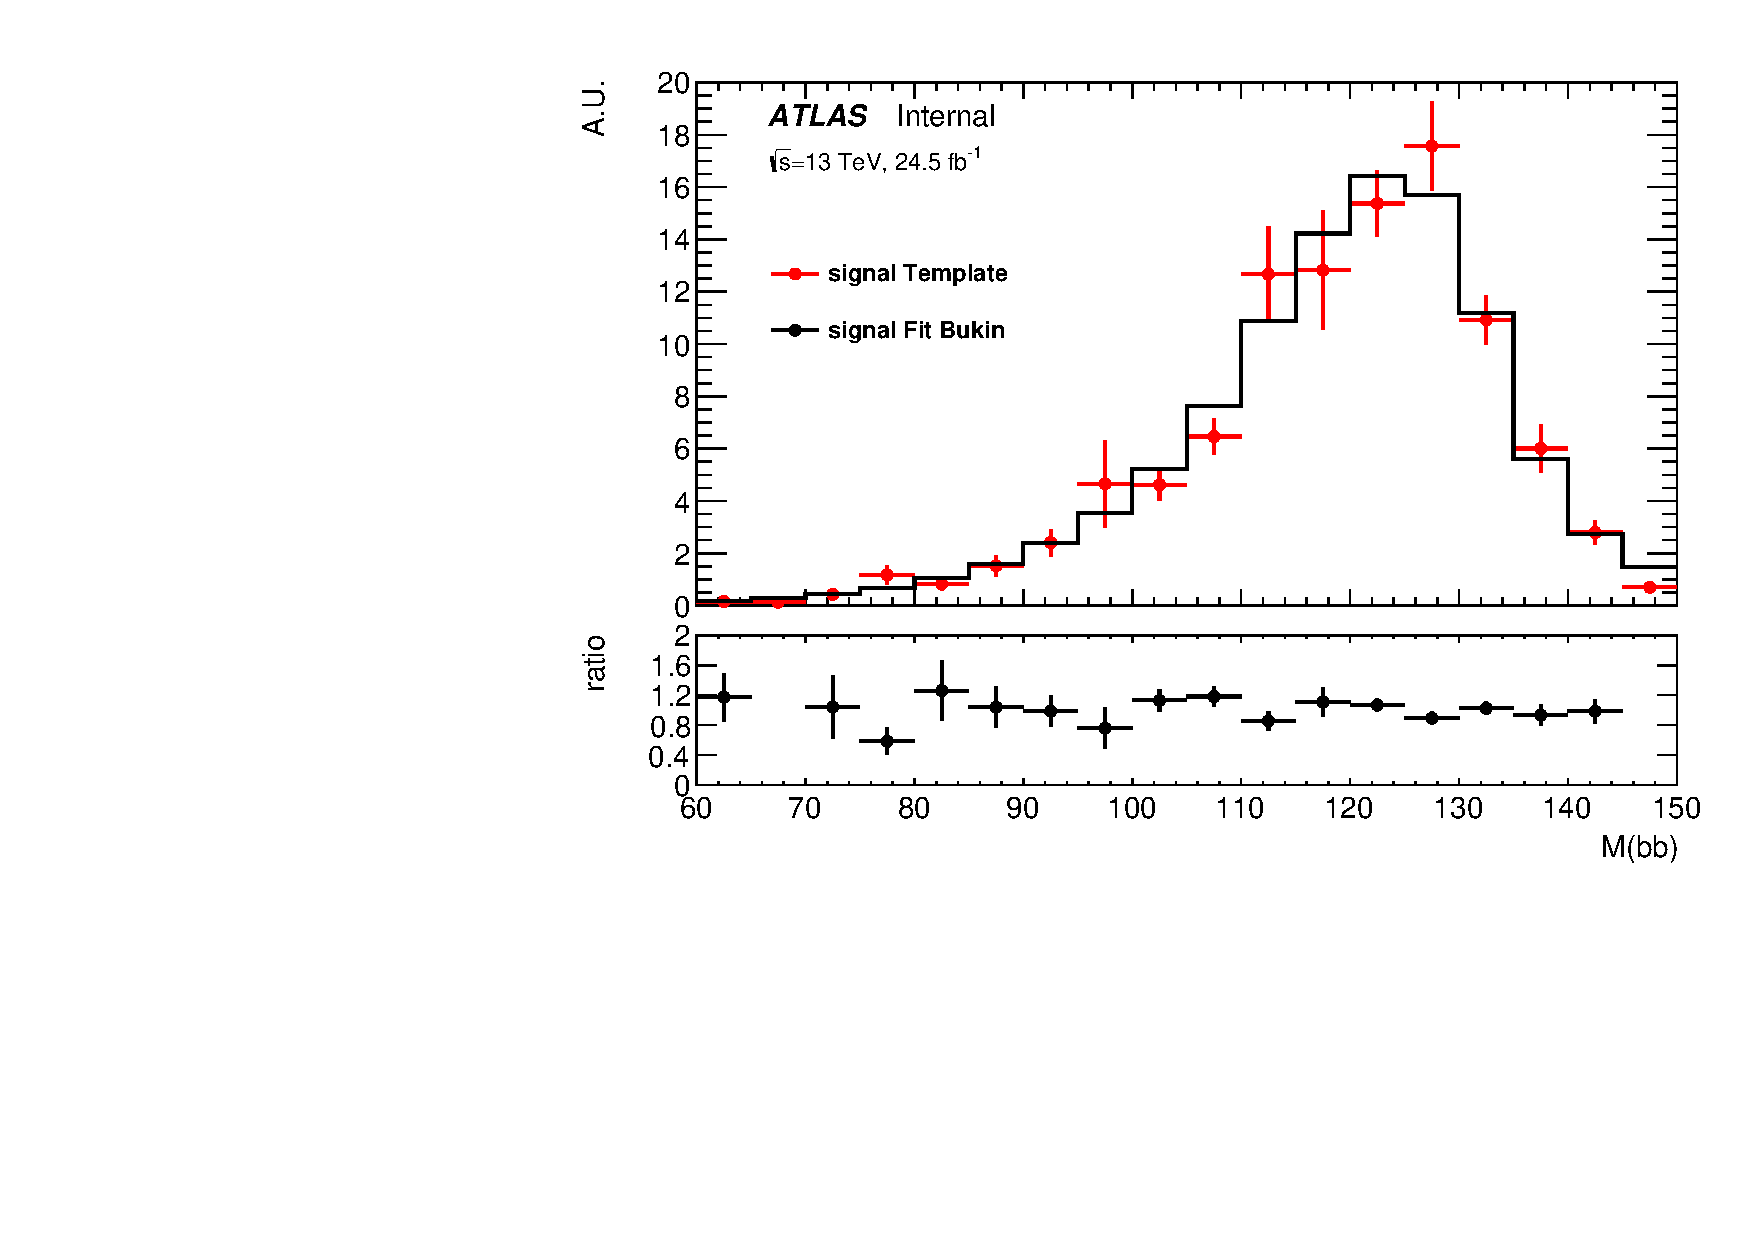
\includegraphics[width=0.24\textwidth]{figures/VBF/sig_4cen_SRIII.pdf}
% 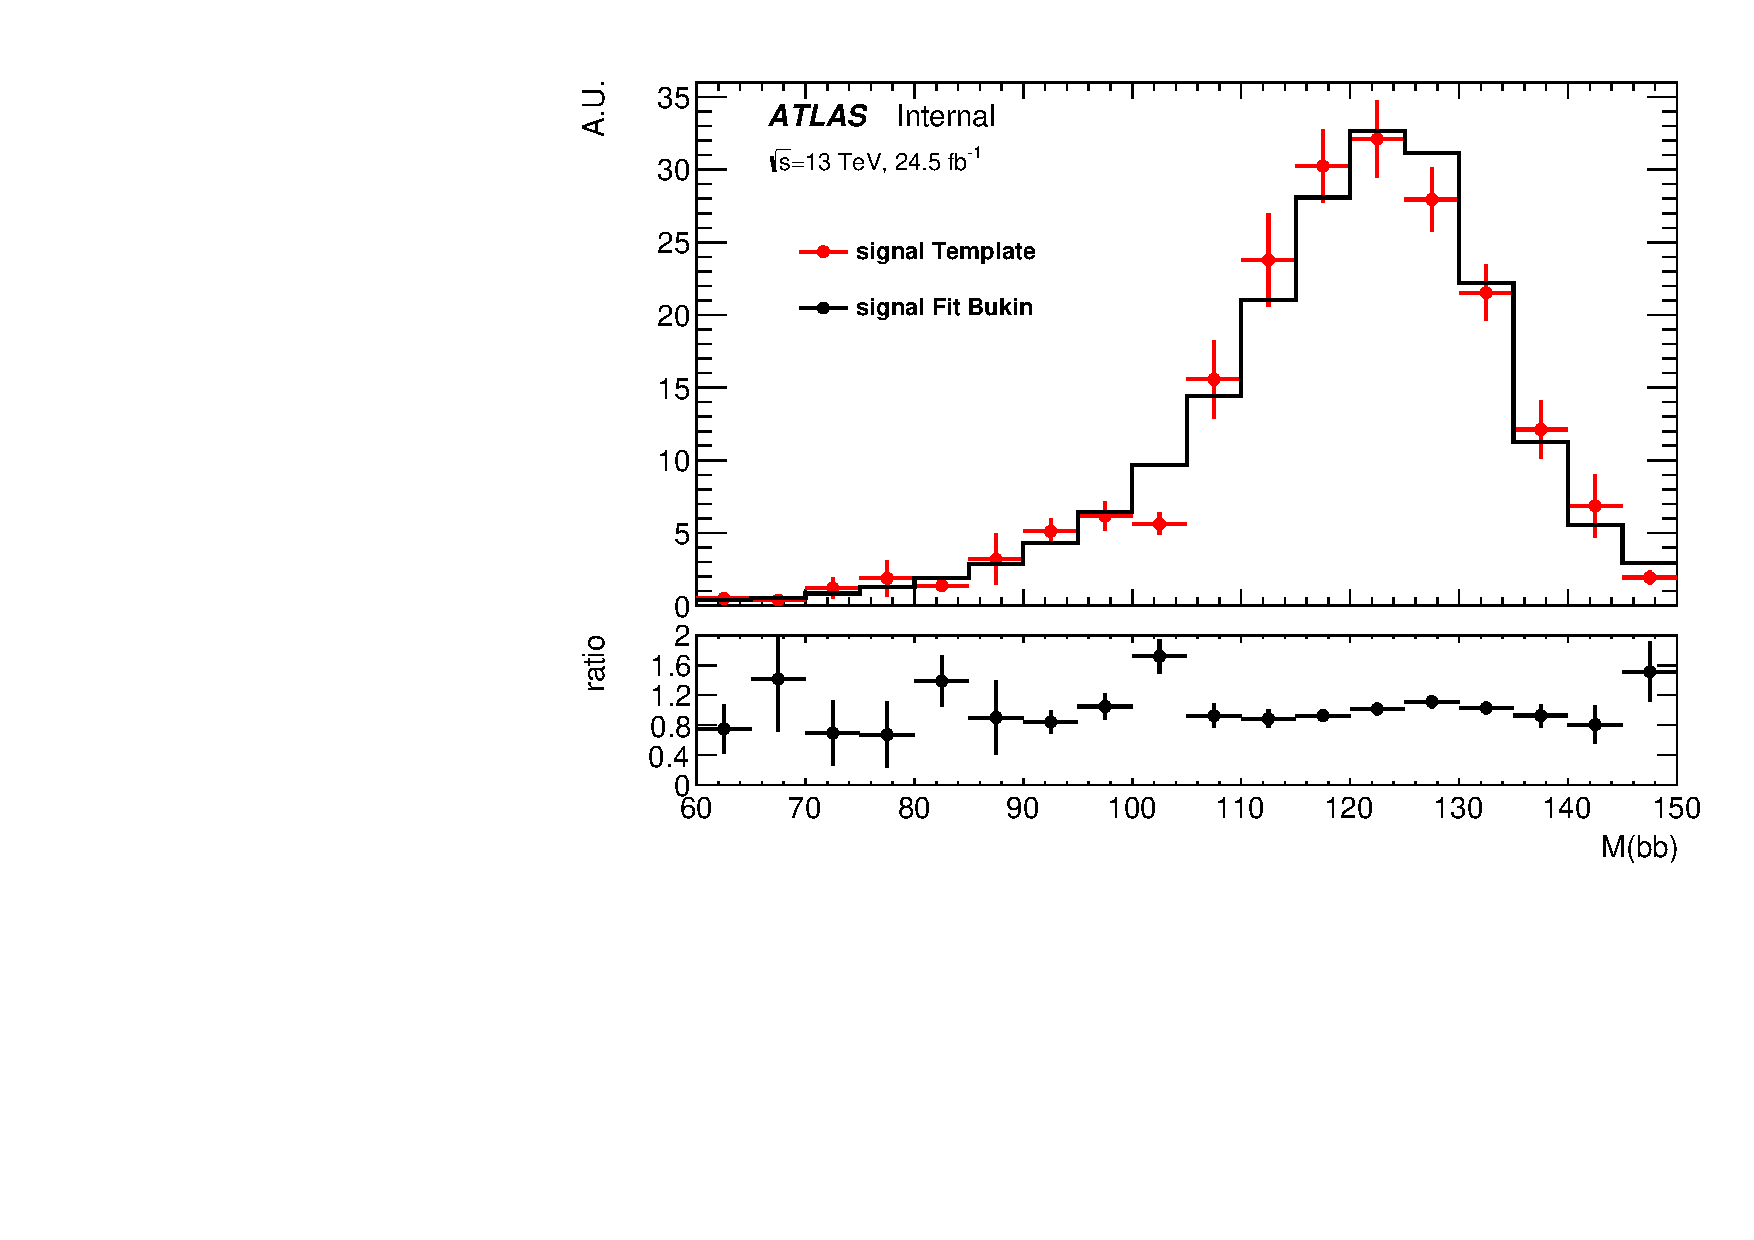
\includegraphics[width=0.24\textwidth]{figures/VBF/sig_4cen_SRIV.pdf}

\caption{Example of Bukin function parametrizations of signal \Mbb{} distributions of SR I in \twocentral channel (left) and SR I in \fourcentral channel (right)}
  \label{fig:vbf-sigpar_alt}
\end{figure}


\begin{figure}[htbp]
  \centering    
 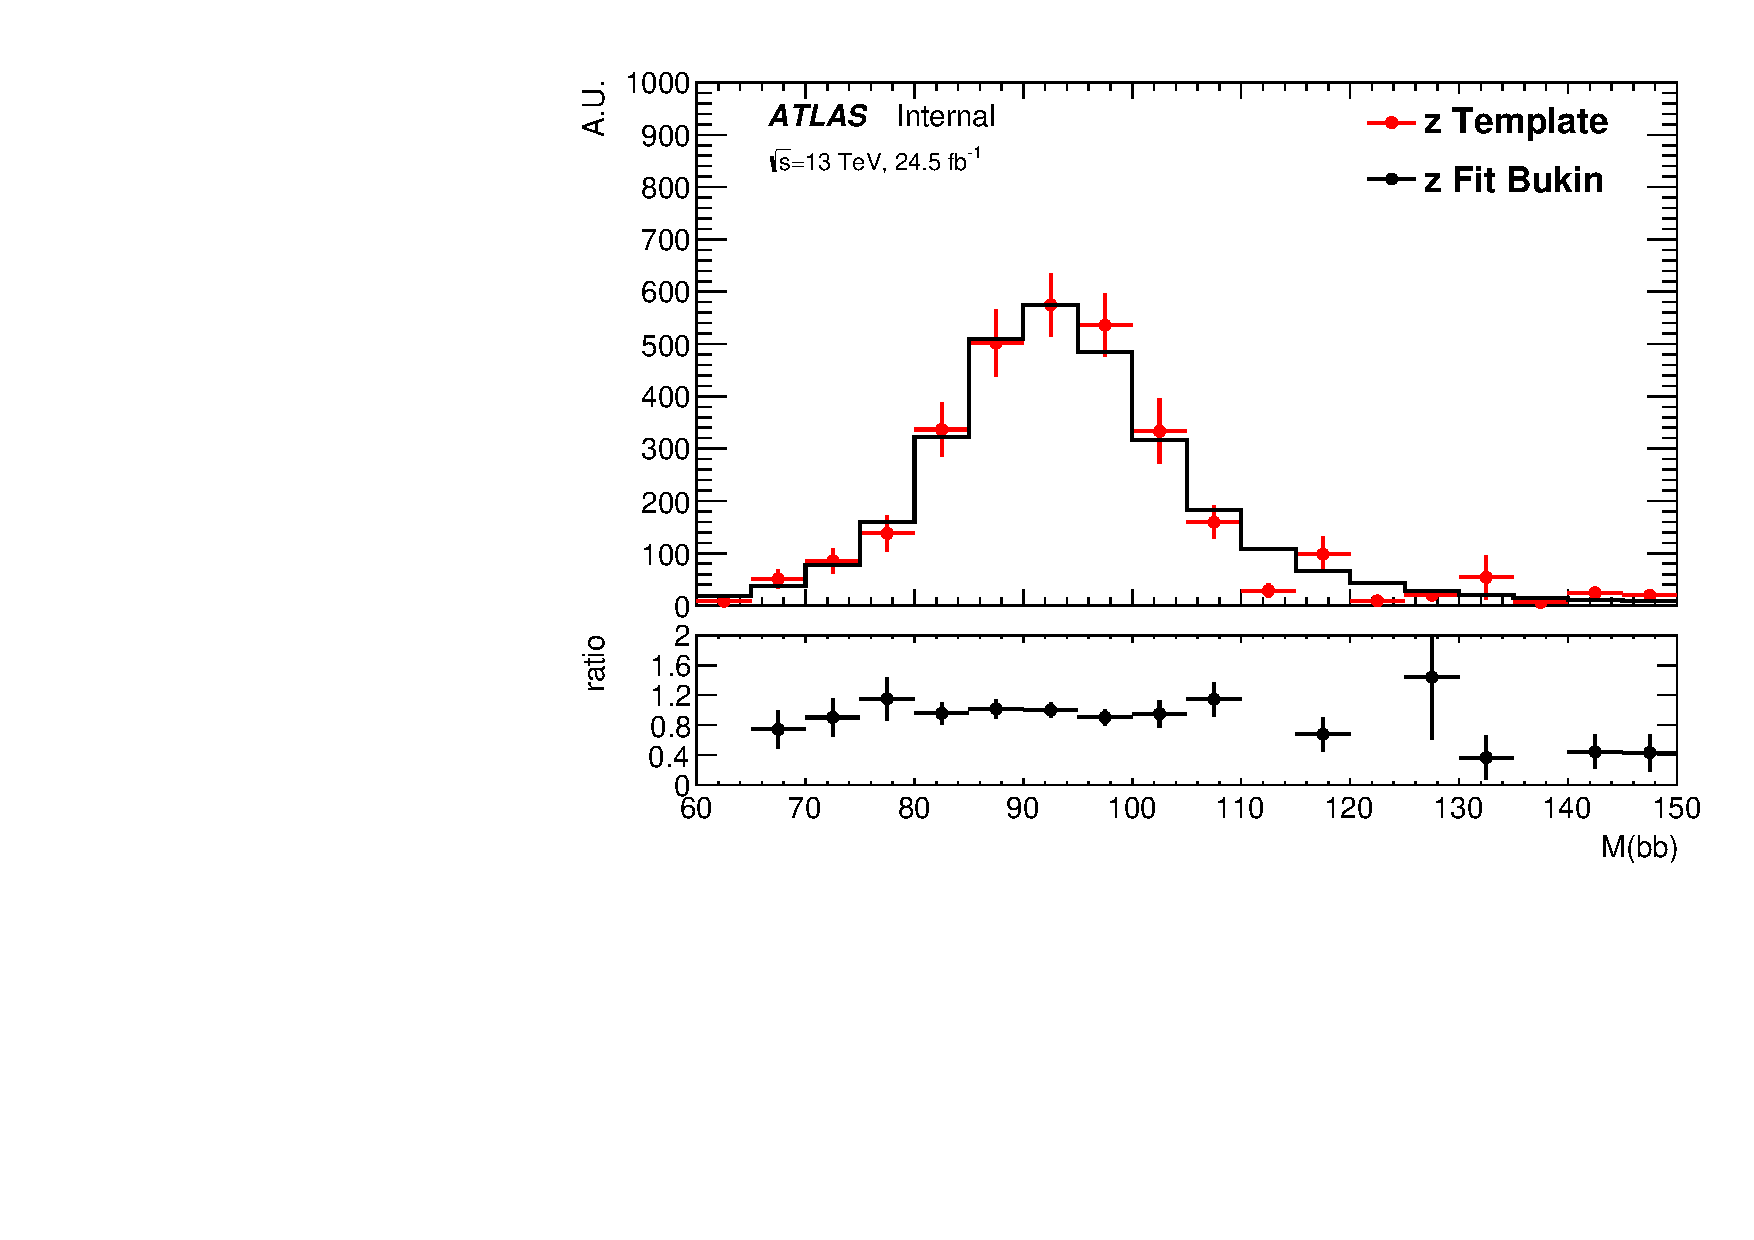
\includegraphics[width=0.45\textwidth]{figures/VBF/SigPar/z_2cen.pdf}
 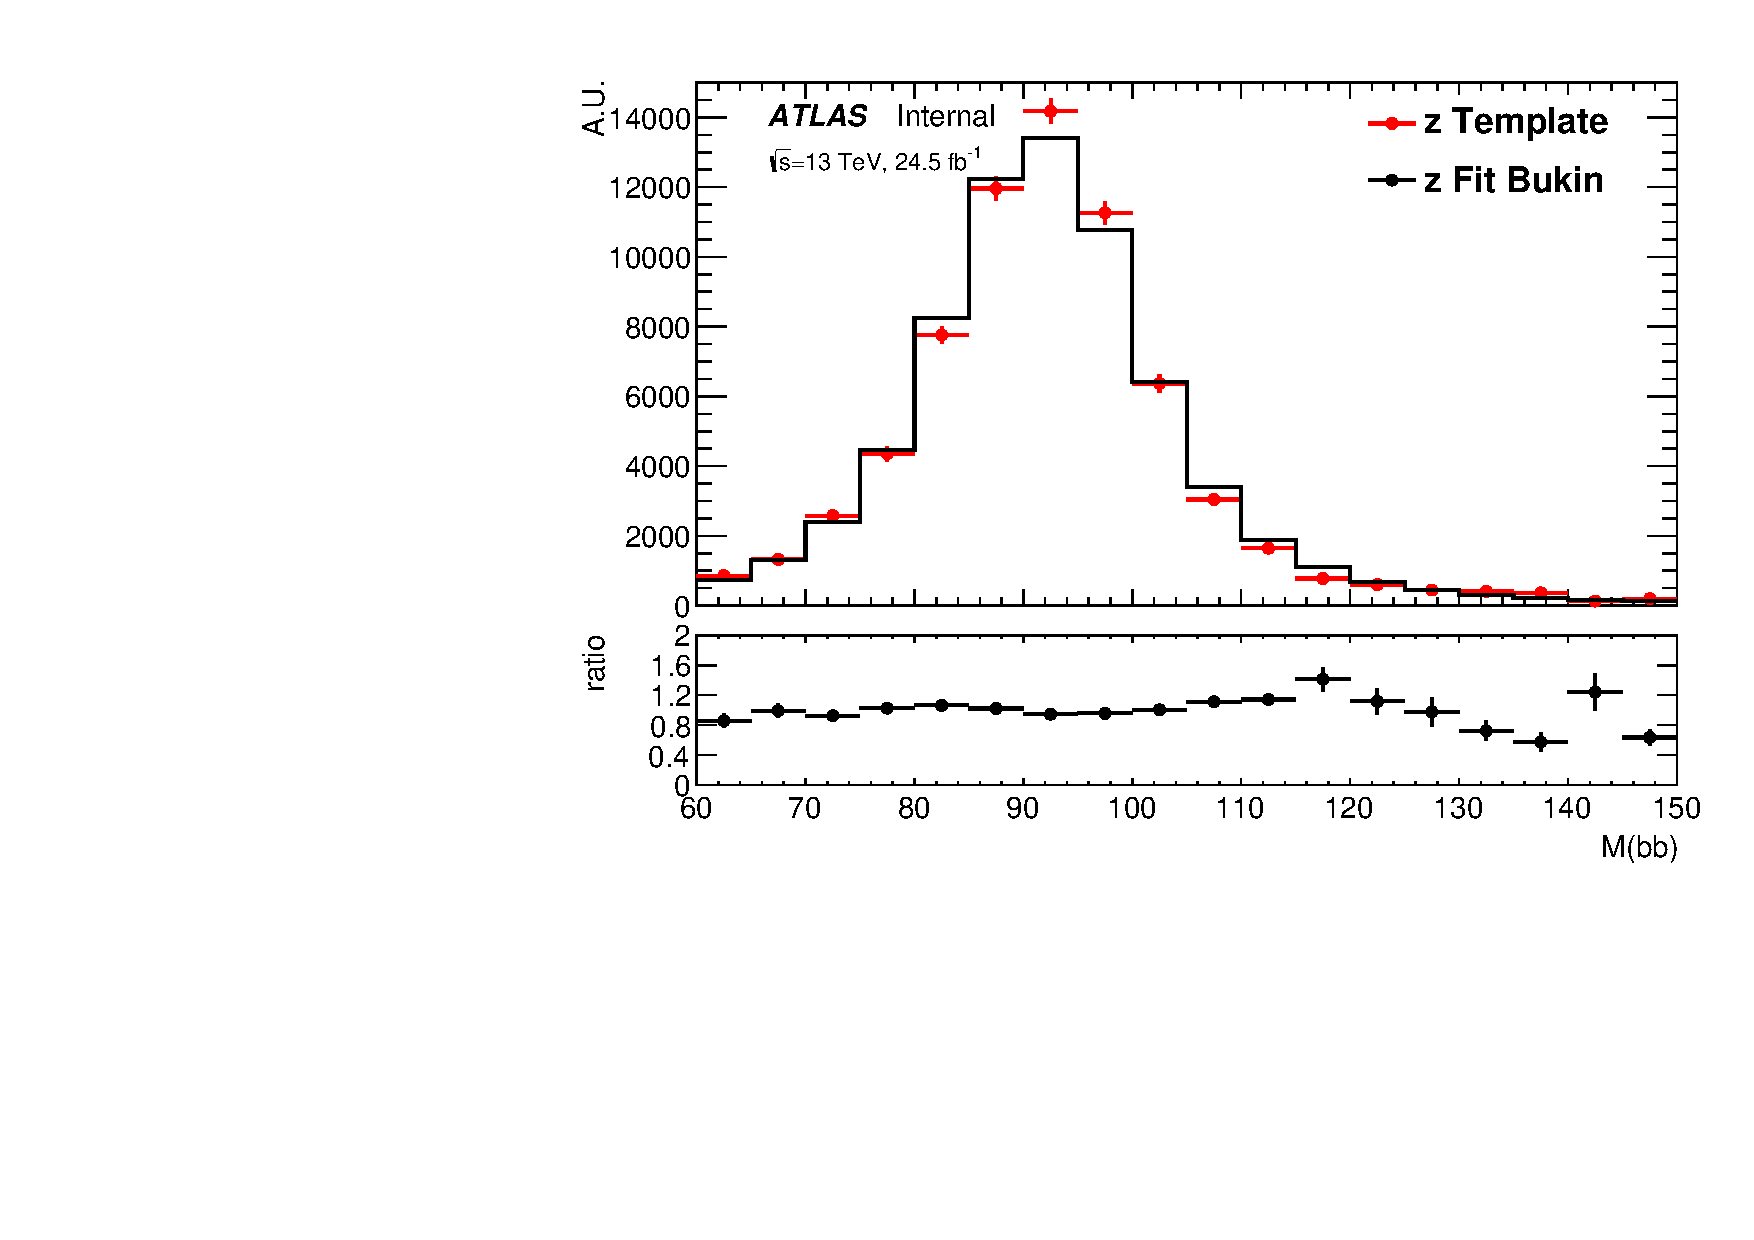
\includegraphics[width=0.45\textwidth]{figures/VBF/SigPar/z_4cen.pdf}

\caption{Bukin function parametrization of \zjets~\Mbb{} distribution in \twocentral (left) and \fourcentral (right). There are not enough events to divide the sample amongst BDT regions, therefore the distributions are shown for each channel preselection.}
\label{fig:vbf-zpar_alt}
\end{figure}



\subsection{Non-resonant Background Estimation}
\label{sec:vbf-nonres}

In order to determine the non-resonant background, we fit  the sidebands of each of the BDT regions independently with an analytical function. The sidebands of the \Mbb{}  distribution of each BDT region are shown in Fig. \ref{fig:vbf-mbb_sidebands}. %An alternative approach  using a control region and a linear transfer factor to relate the control region shape to the signal regions is documented in Appendix~\ref{sec:vbf-app-oldfitbkgds}.  However, due to concerns about the validity of the approach, documented in Appendix~\ref{sec:vbf-app-LinearityTest}, the more conservative approach of independent fits is taken here.  

\begin{figure}[htbp]
  \centering
 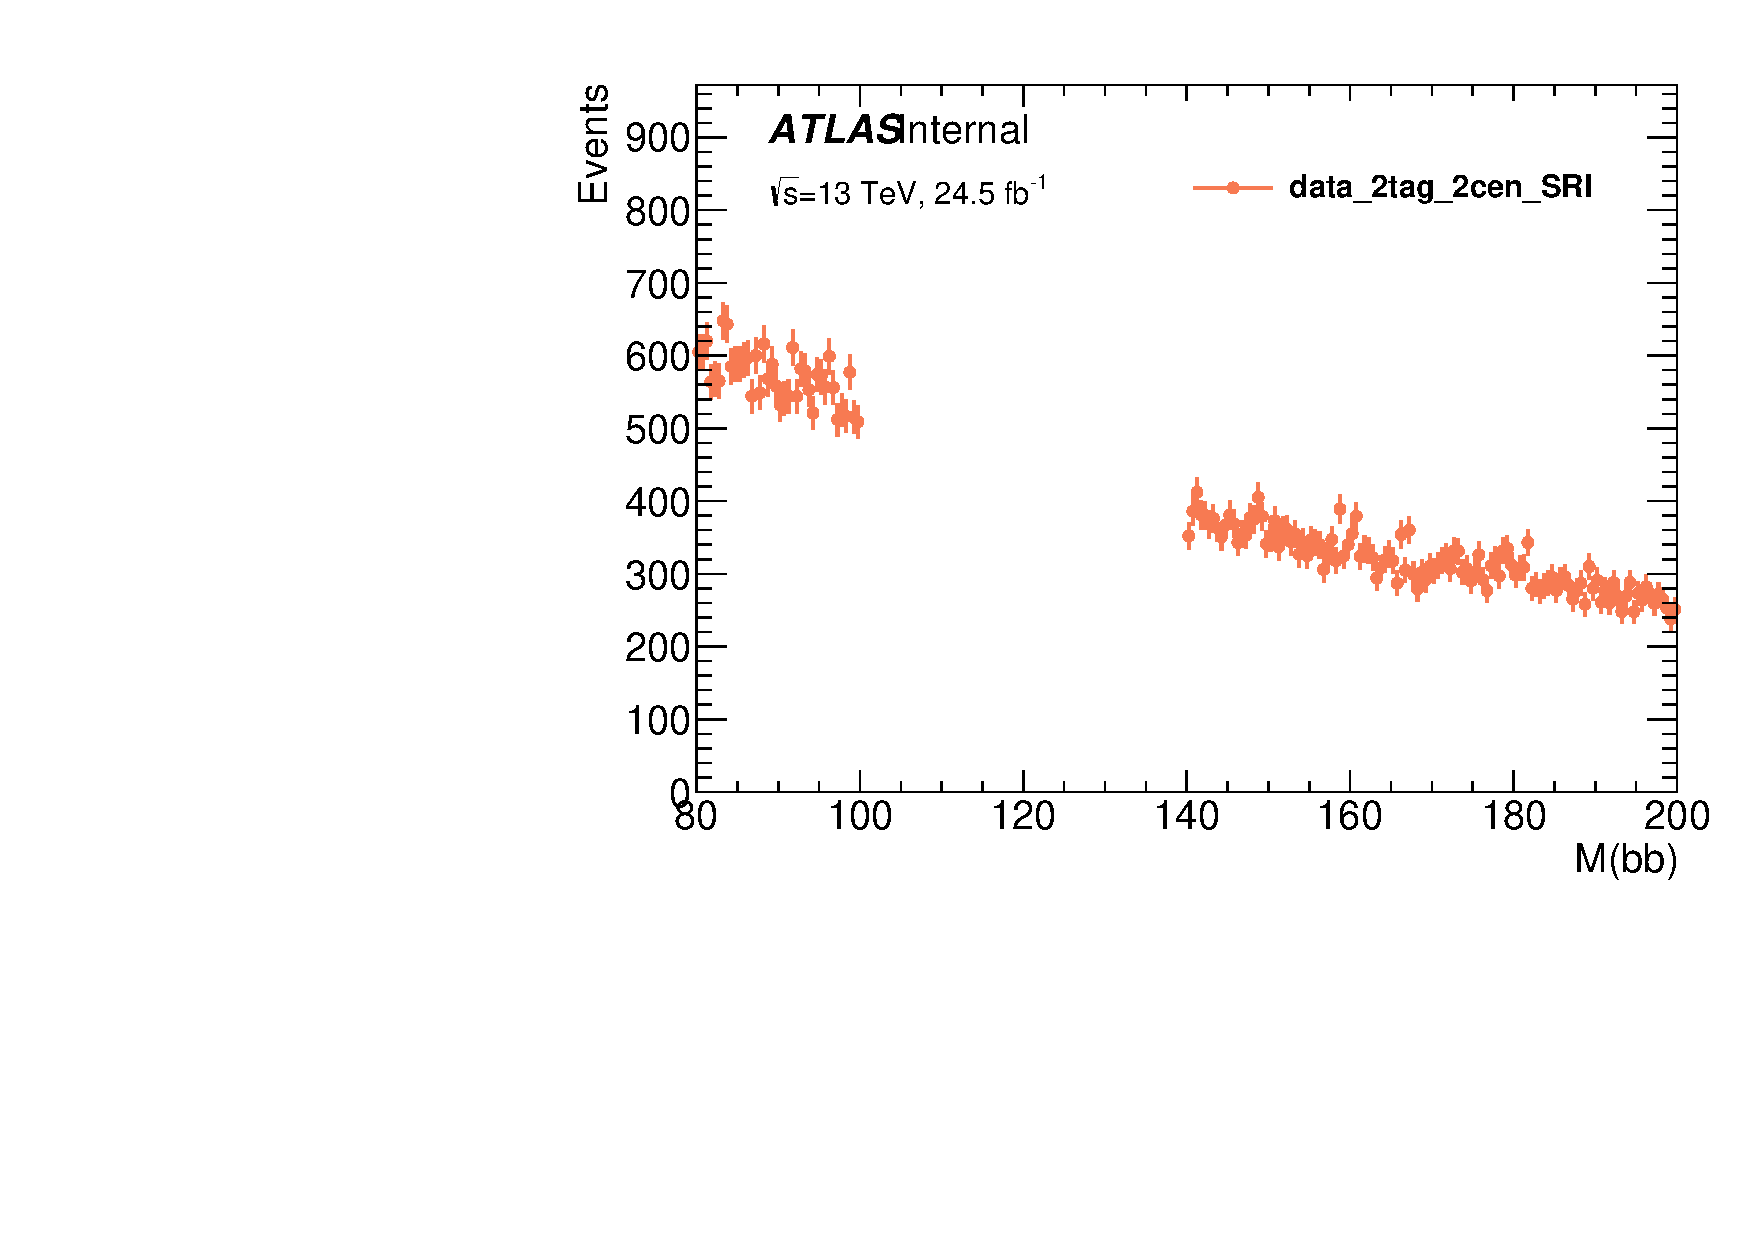
\includegraphics[width=0.45\textwidth]{figures/VBF/Mbb_SRI_2cen.pdf}
 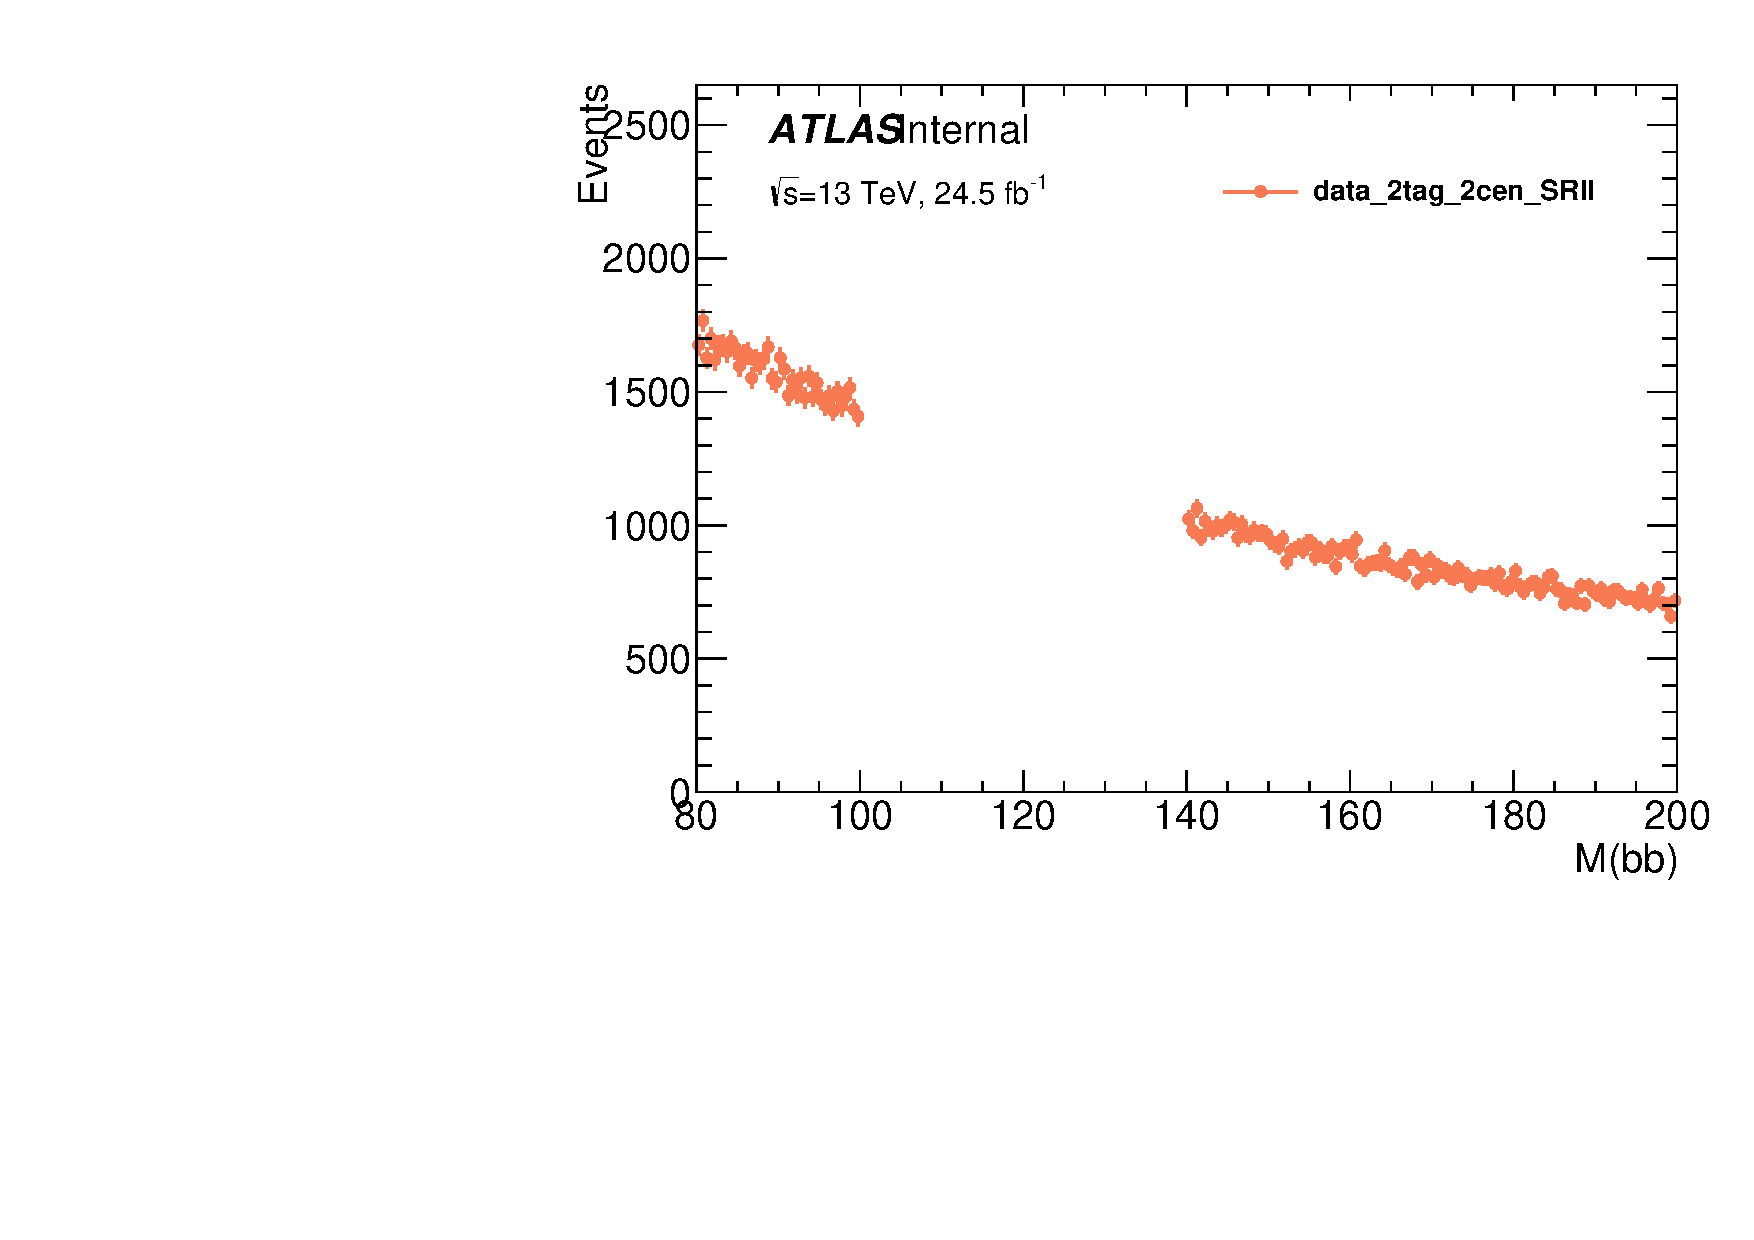
\includegraphics[width=0.45\textwidth]{figures/VBF/Mbb_SRII_2cen.pdf}\\
 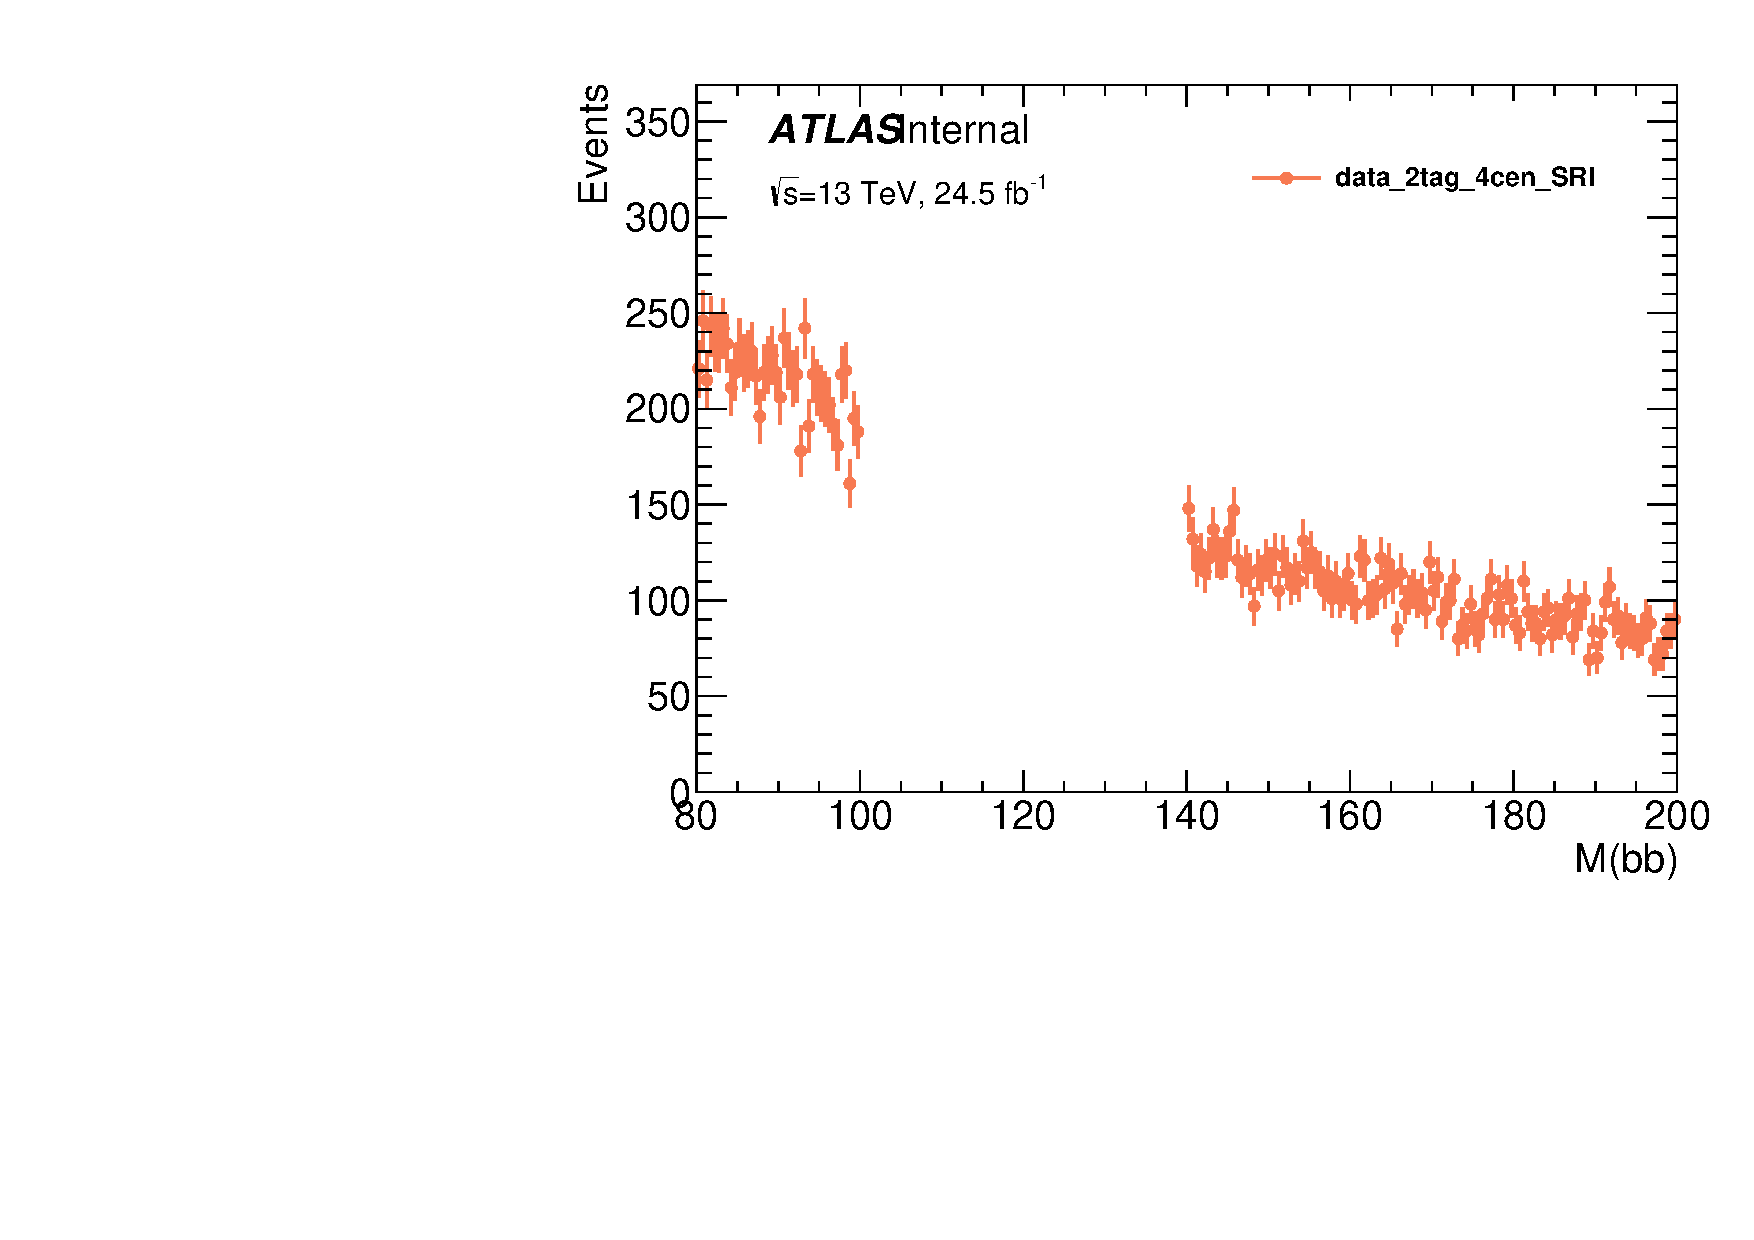
\includegraphics[width=0.45\textwidth]{figures/VBF/Mbb_SRI_4cen.pdf}
 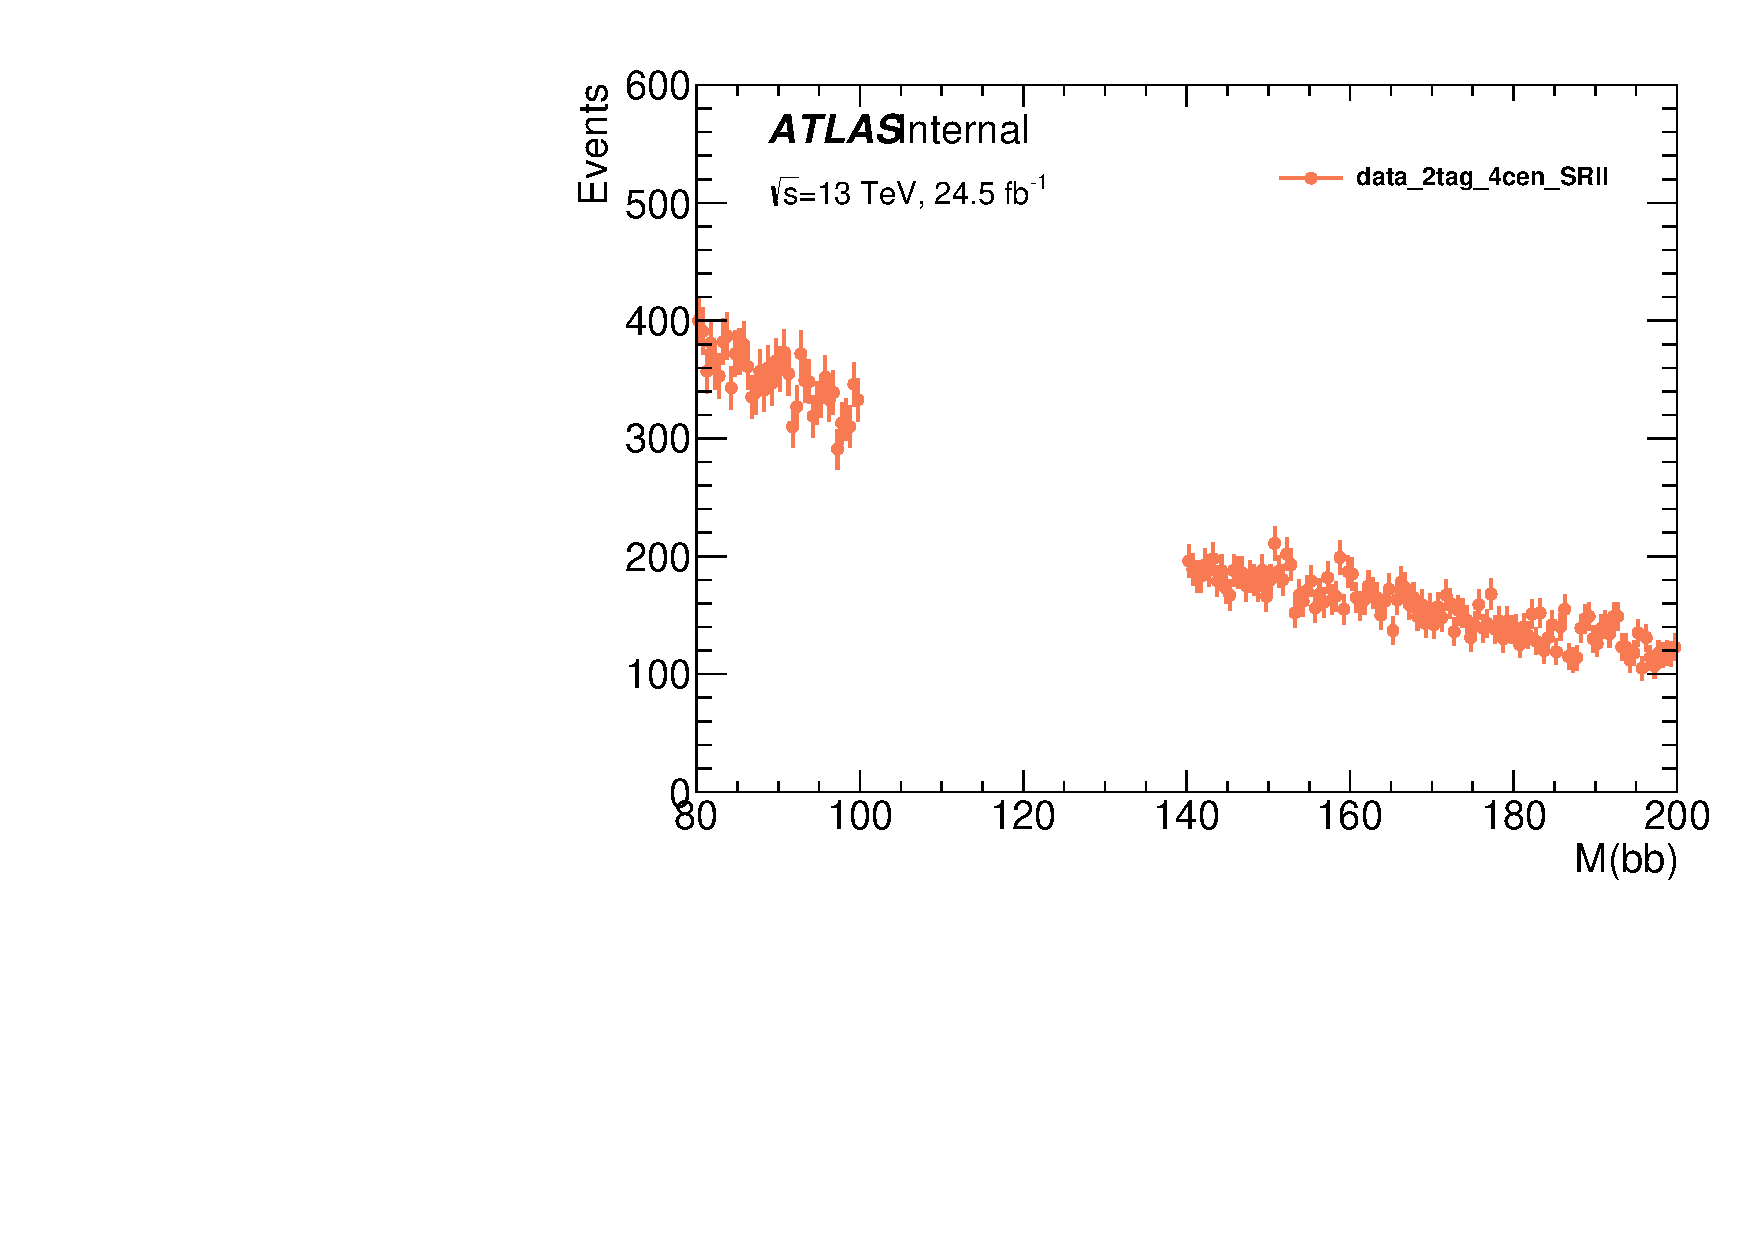
\includegraphics[width=0.45\textwidth]{figures/VBF/Mbb_SRII_4cen.pdf}\\
 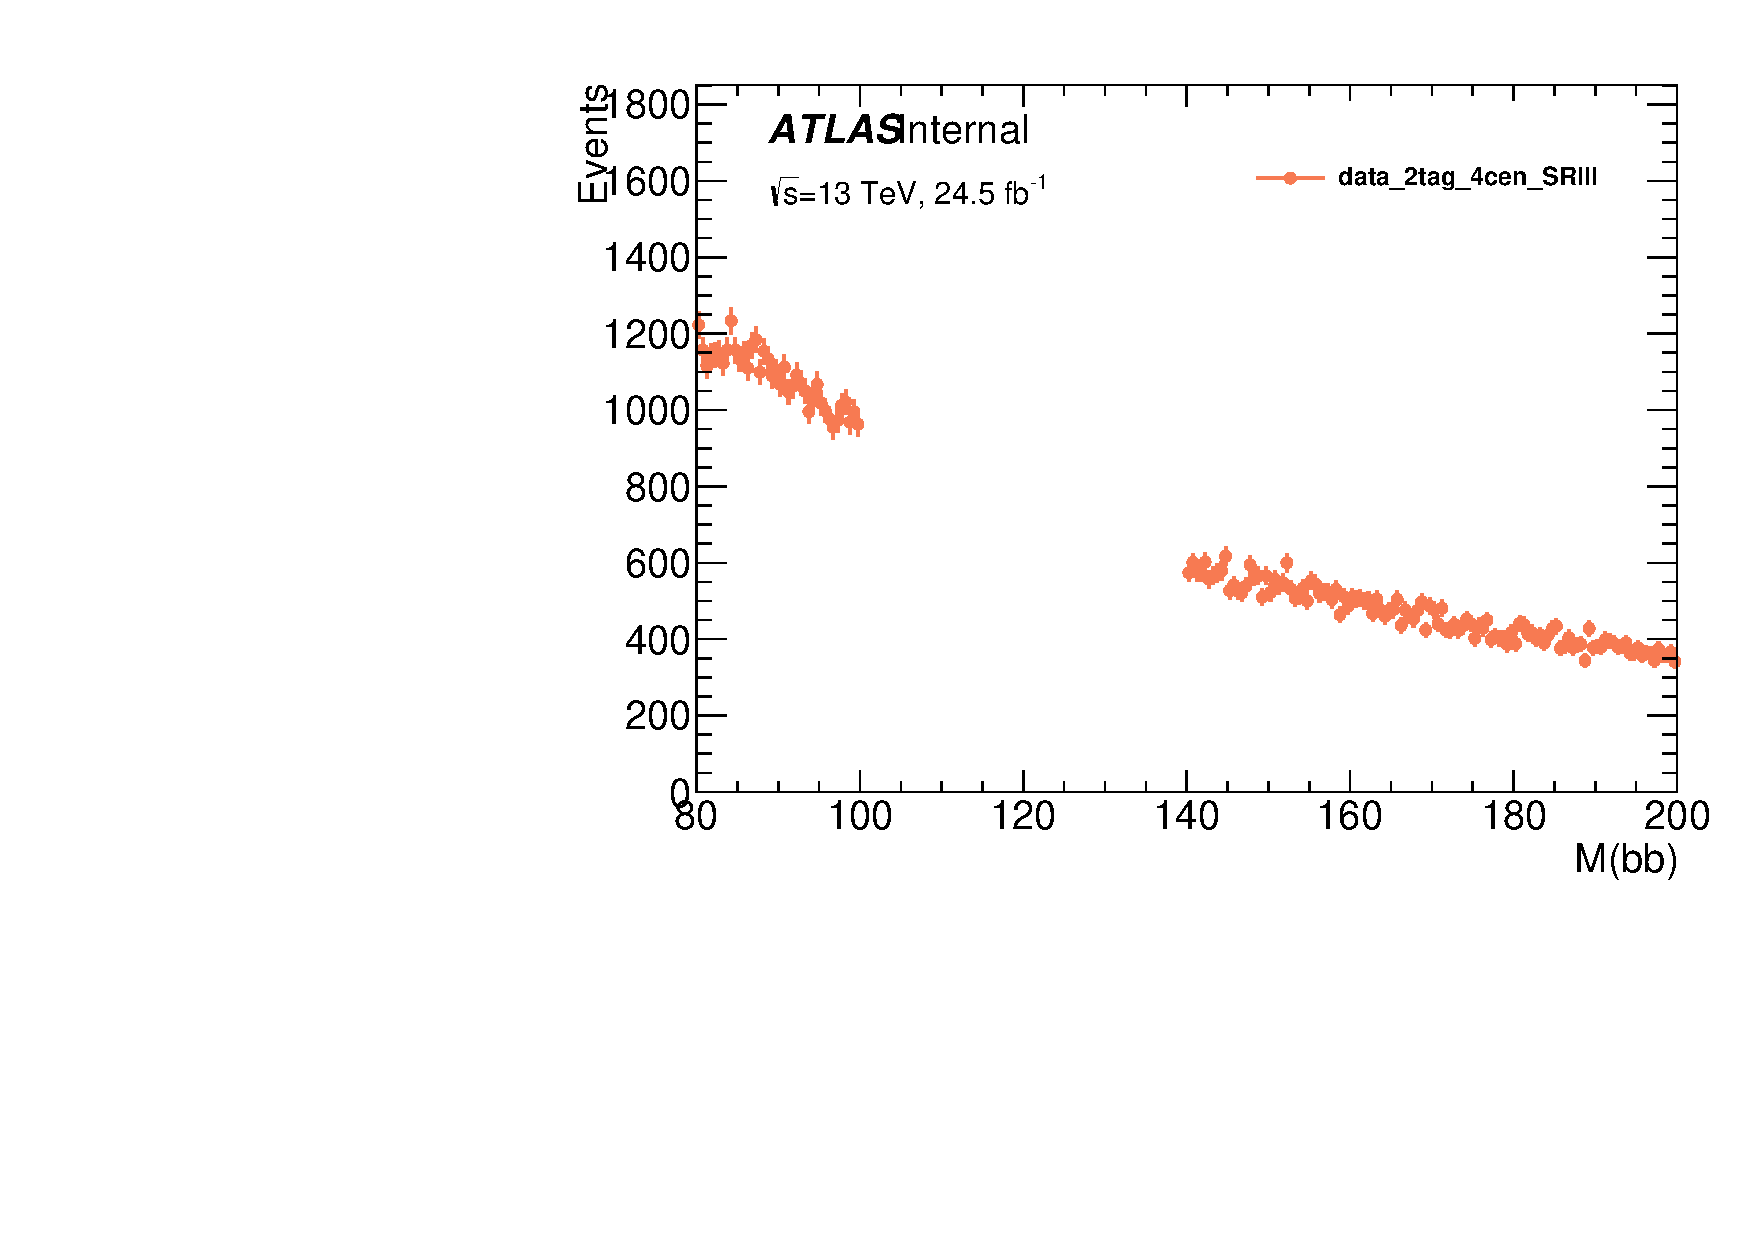
\includegraphics[width=0.45\textwidth]{figures/VBF/Mbb_SRIII_4cen.pdf}
 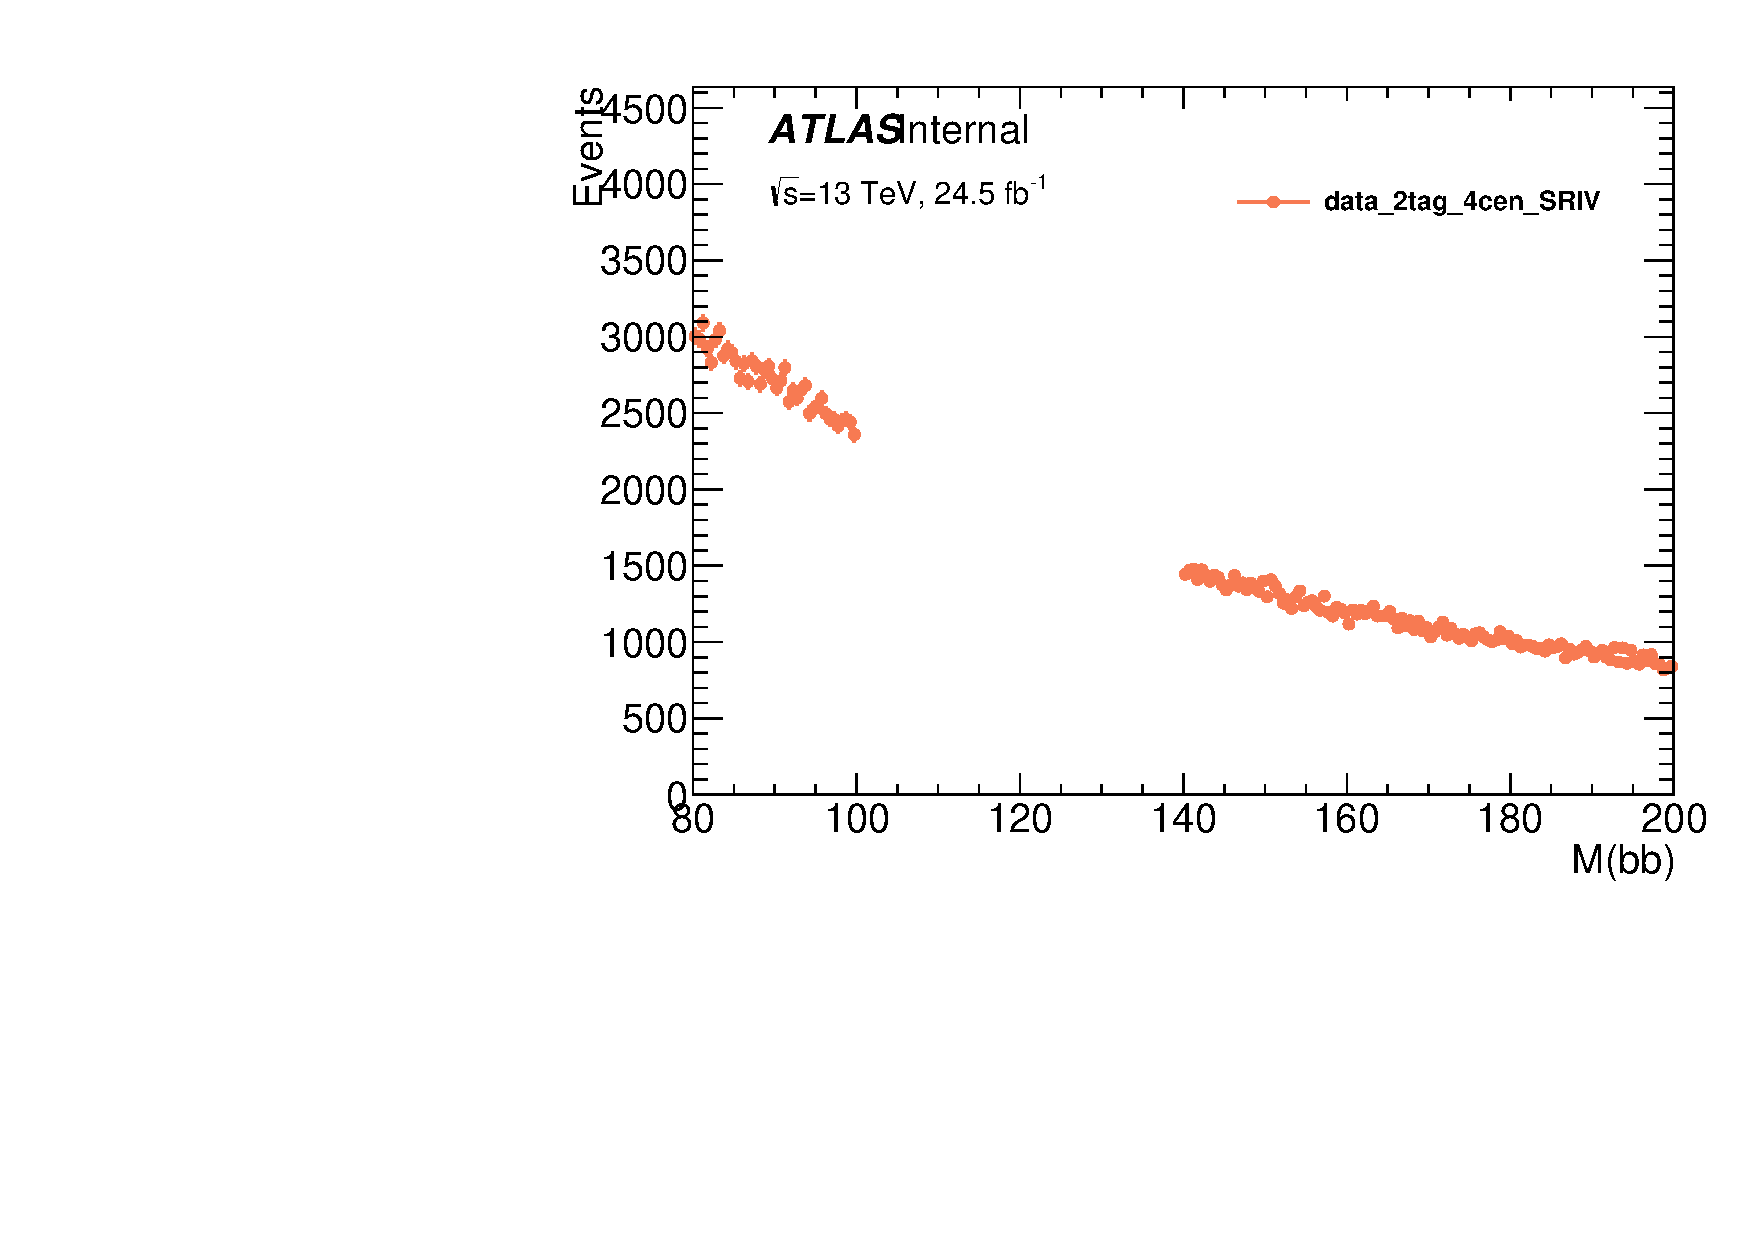
\includegraphics[width=0.45\textwidth]{figures/VBF/Mbb_SRIV_4cen.pdf}\\
\caption{\Mbb{} shapes of all BDT regions in sidebands} 
  \label{fig:vbf-mbb_sidebands}
\end{figure}


Several function families are considered and tested. The primary family of functions considered is that of the Bernstein polynomials listed in Equation~\ref{eq:bernstein}, which were
used successfully in the previous iteration of this analysis. The product of Bernstein and exponential functions, as well as the sum of exponentials, were used as the alternative functions for background description.
The functions chosen are required to pass two conditions. Among the candidates satisfying the conditions above, the function with the smallest number of degrees of freedom is chosen.

\begin{itemize}
\item 
Compatibility: The function must be statistically  compatible with the sidebands of the \Mbb{} distribution in the signal regions, where the Higgs mass range $100<\Mbb<140$ GeV is ignored. The compatibility criterion is defined as $P(\chi^2)>0.05$ and $P(F-\rm{test})>0.05$,  where the $\chi^2$ and $F-\rm{test}$ probabilities are considered, respectively. The $F-\rm{test}$ is performed with respect to the $n+1$ order function.  Only statistical errors are considered in these fits.  Among the candidates satisfying the conditions above, the function with the smallest number of degrees of freedom is chosen. For this study, the \zjets{} component is included in the fit,  normalized to the SM prediction.

\item Spurious Signal:  The lowest order function that satisfies compatibility condition, $f_{B}$, is tested against the the lowest order functions in an alternative truth model, $f_{A}$, that also satisfies the compatibility condition, to derive the spurious signal size \cite{CMS-HIG-12-028}. This is a standard approach used for similar analysis. Although in the future this approach needs better understanding if it double counts partial statistical uncertainty of data, we adopt this apporach to be conservative in estimating uncertainty. We build pseudo data from $f_{A}$, where the parameters of the function are derived from the fit to the sidebands in each signal region.  We then fit the distribution with $f_{B}$ plus $\mu_{sp}$ times the signal template. The measured  apparent signal size needs to be less than $50\%$ of the actual signal size. If this test fails, the the next order function satisfying the compatibility condition is tested.  The \zjets{} component is not included in the pseudo data.

\end{itemize}


The $\chi^2$ values and probabilities and $F-\rm{test}$ probabilities are summarized in Tables~\ref{tab:chi2-2cen} through~\ref{tab:f-test}. The $\chi^2$ test criteria are met for the O(2) Bernstein function in all regions, except in 
SR IV of the \fourcentral channel where we need at least an O(3) Bernstein function. The $F$-test is passed for functions which pass the $\chi^2$ criterion in all channels and regions.

The spurious signal fits are given in Tables~\ref{tab:spurious-test-2cen} and~\ref{tab:spurious-test-4cen}, which additionally show which functions are used as the alternative truth models. In most regions the O(3) Bernstein polynomial satisfies the spurious signal criterion. Note that our choice of background function minimizes the potential bias in trade of variance, i.e. the higher order functional forms yield larger uncertainty.

To satisfy all of the criteria, we choose an O(3) Bernstein function for the \twocentral channels, as well as for all SRs of the \fourcentral channel except SR IV which uses O(4).  


%\begin{figure}[htbp]
%  \centering
% 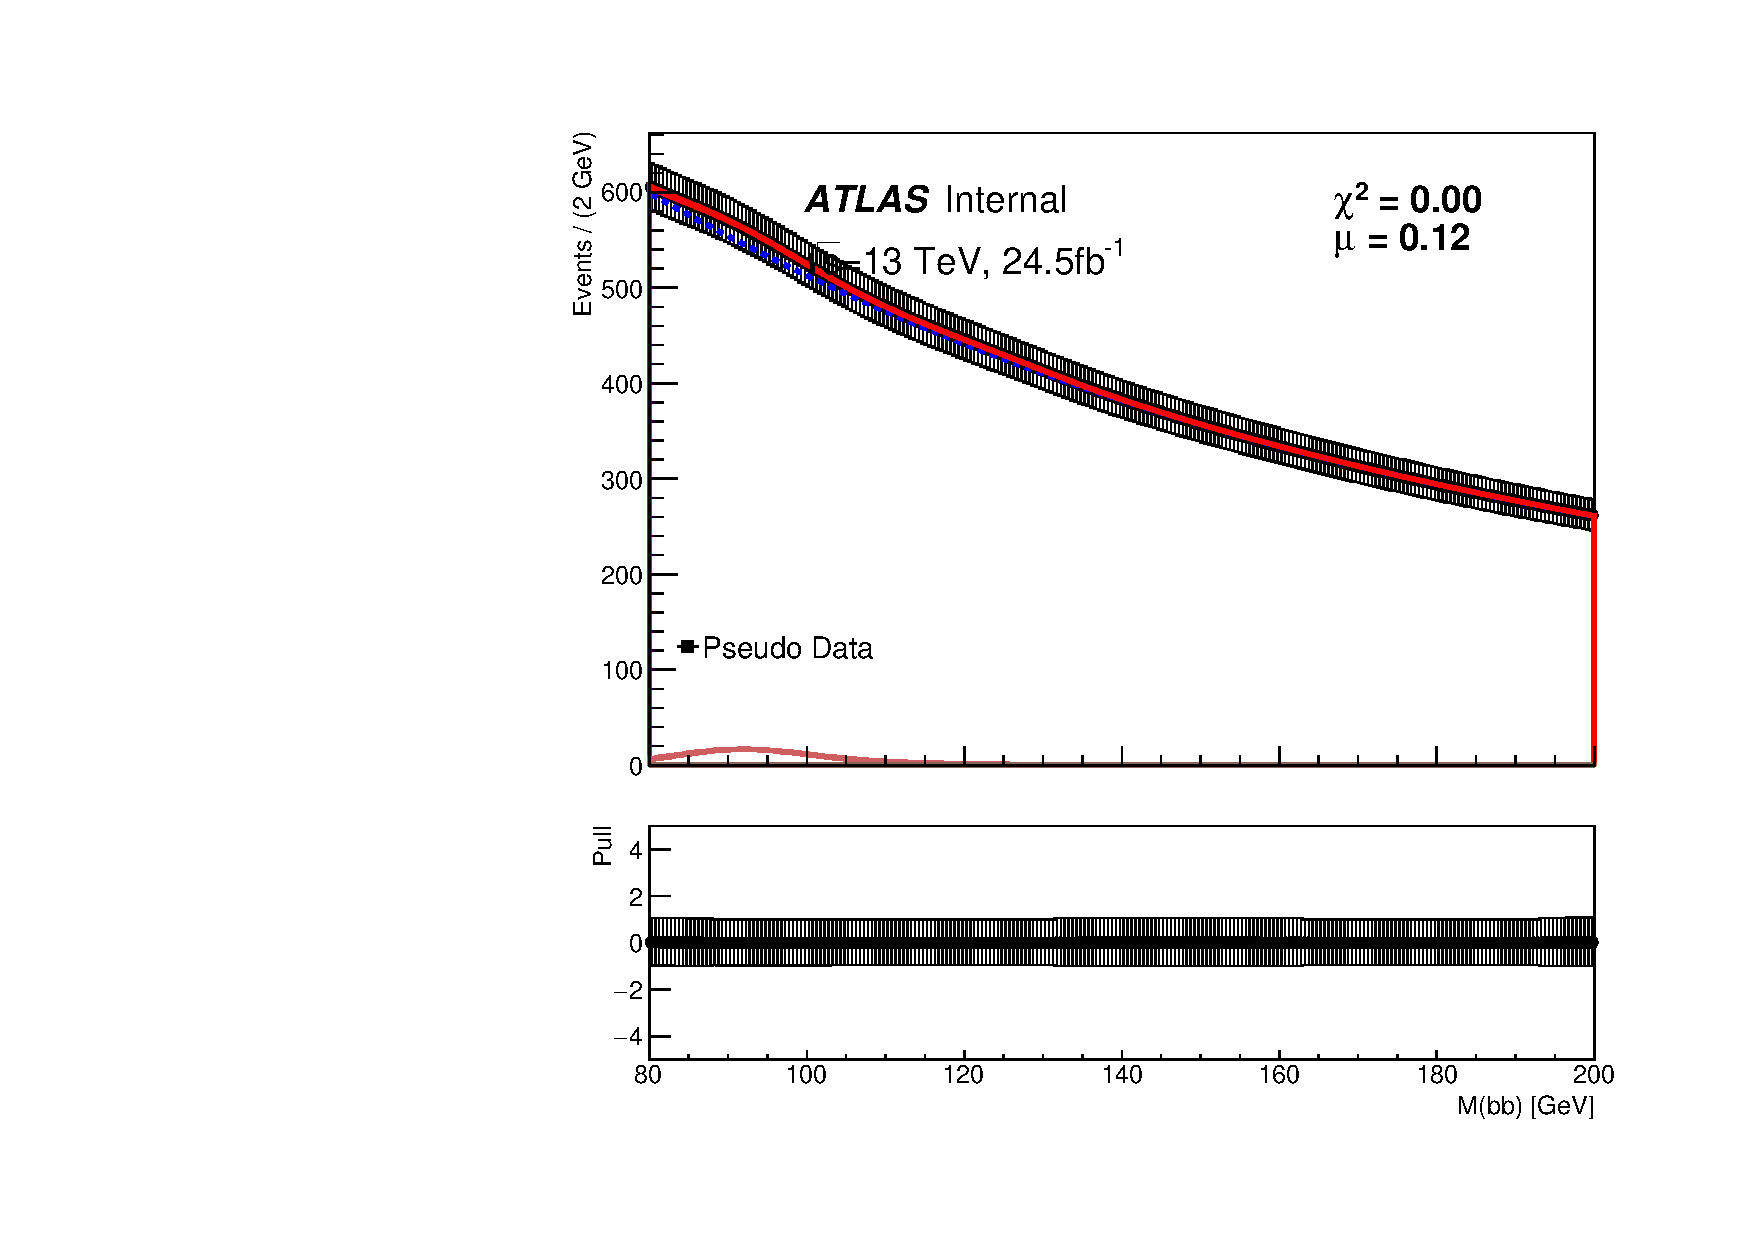
\includegraphics[width=0.24\textwidth]{figures/VBF/Spurious_ExpoO2_testVBF_ICHEP_2cen_SRI.pdf}
% 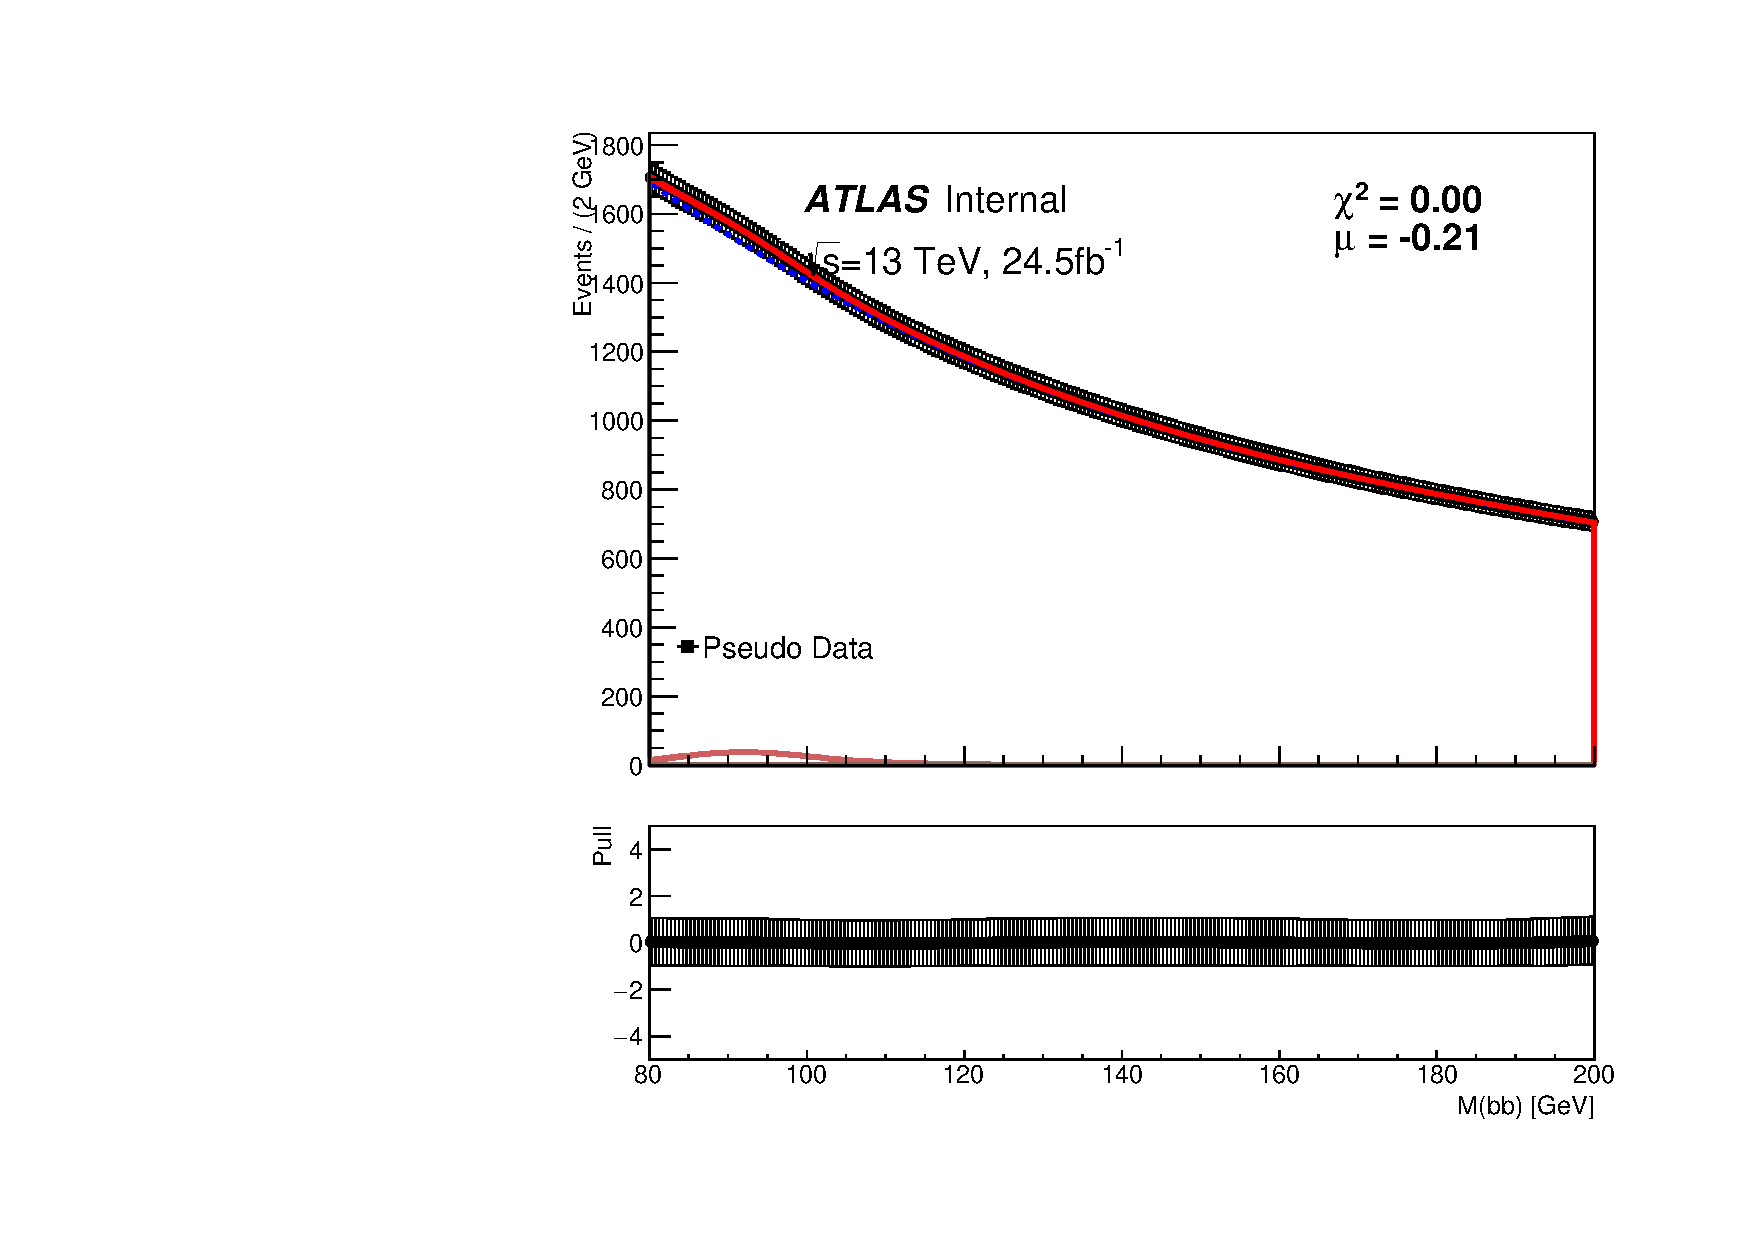
\includegraphics[width=0.24\textwidth]{figures/VBF/Spurious_ExpoO2_testVBF_ICHEP_2cen_SRII.pdf}\\
% 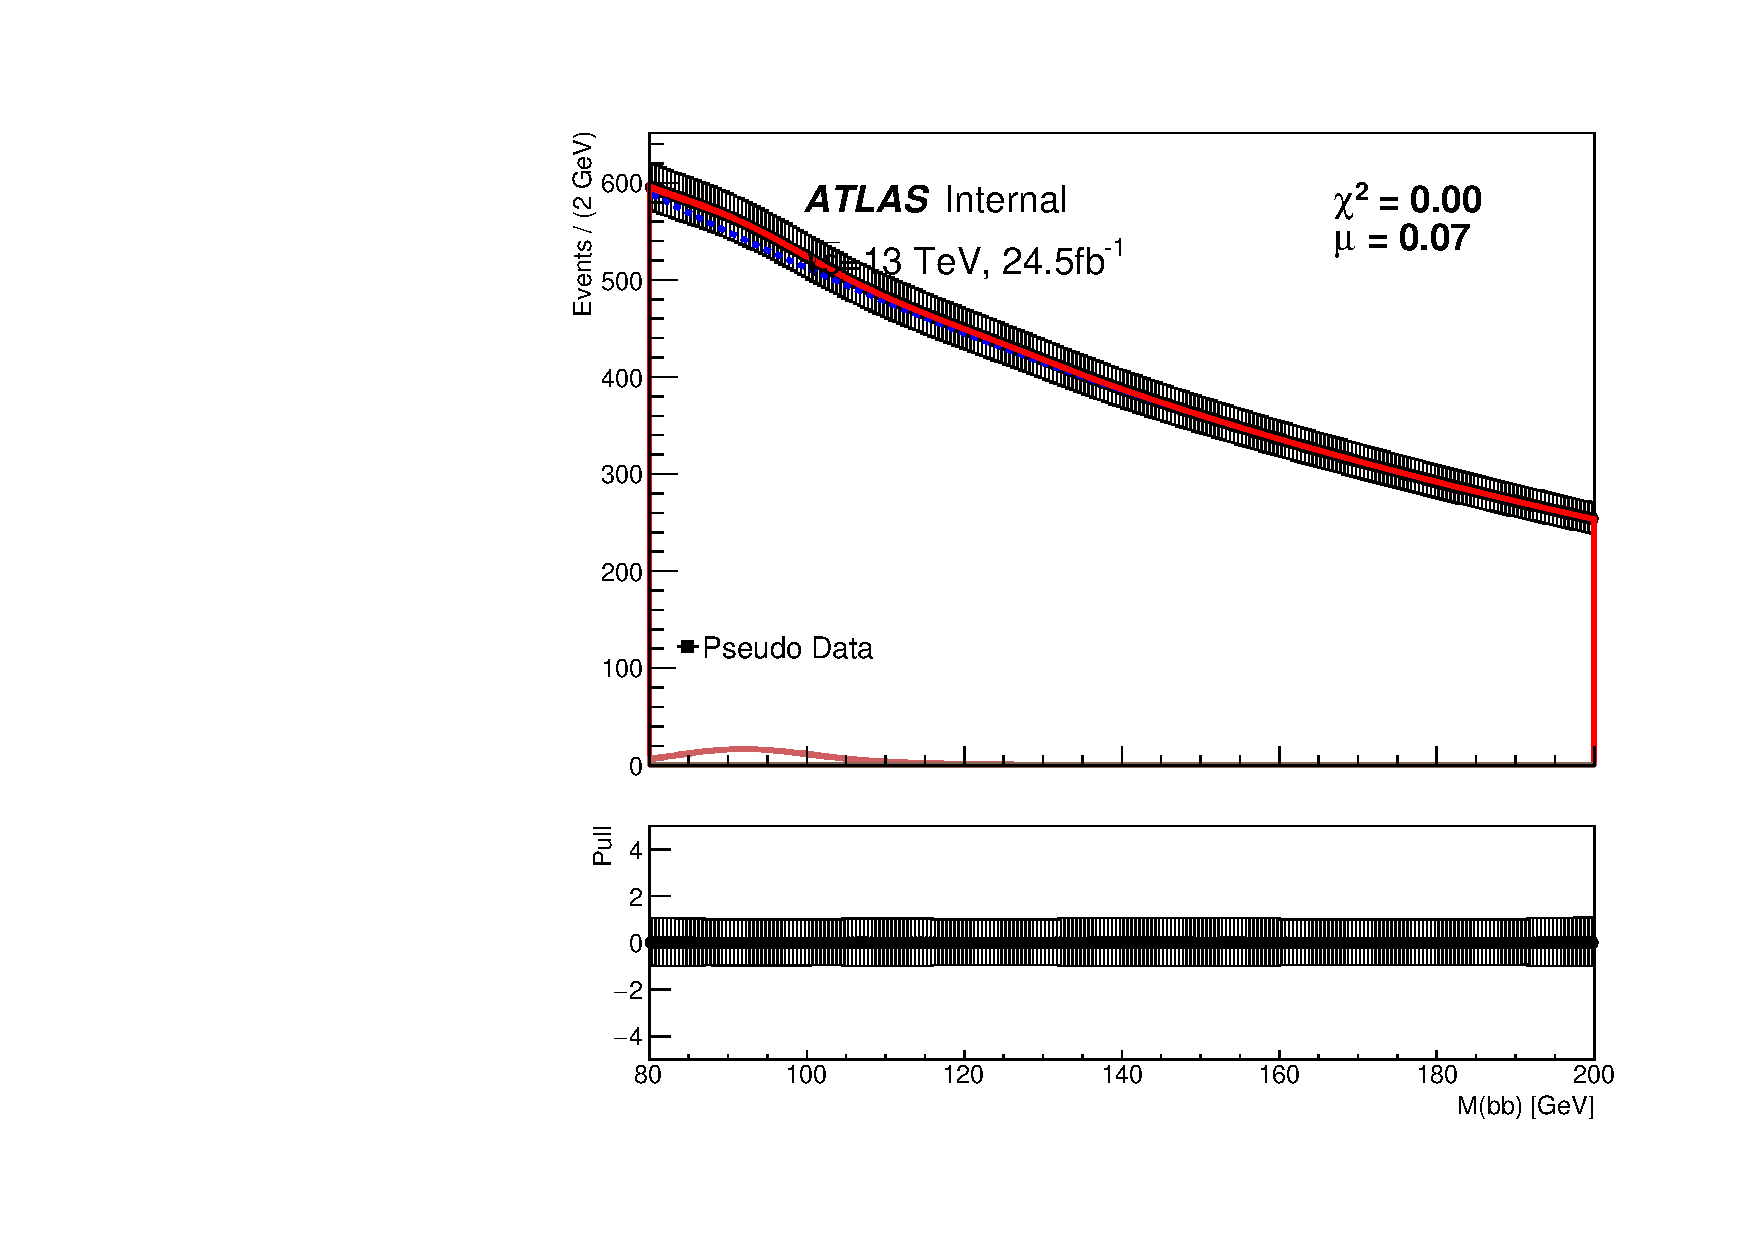
\includegraphics[width=0.24\textwidth]{figures/VBF/Spurious_SExpoO2_testVBF_ICHEP_2cen_SRI.pdf}
% 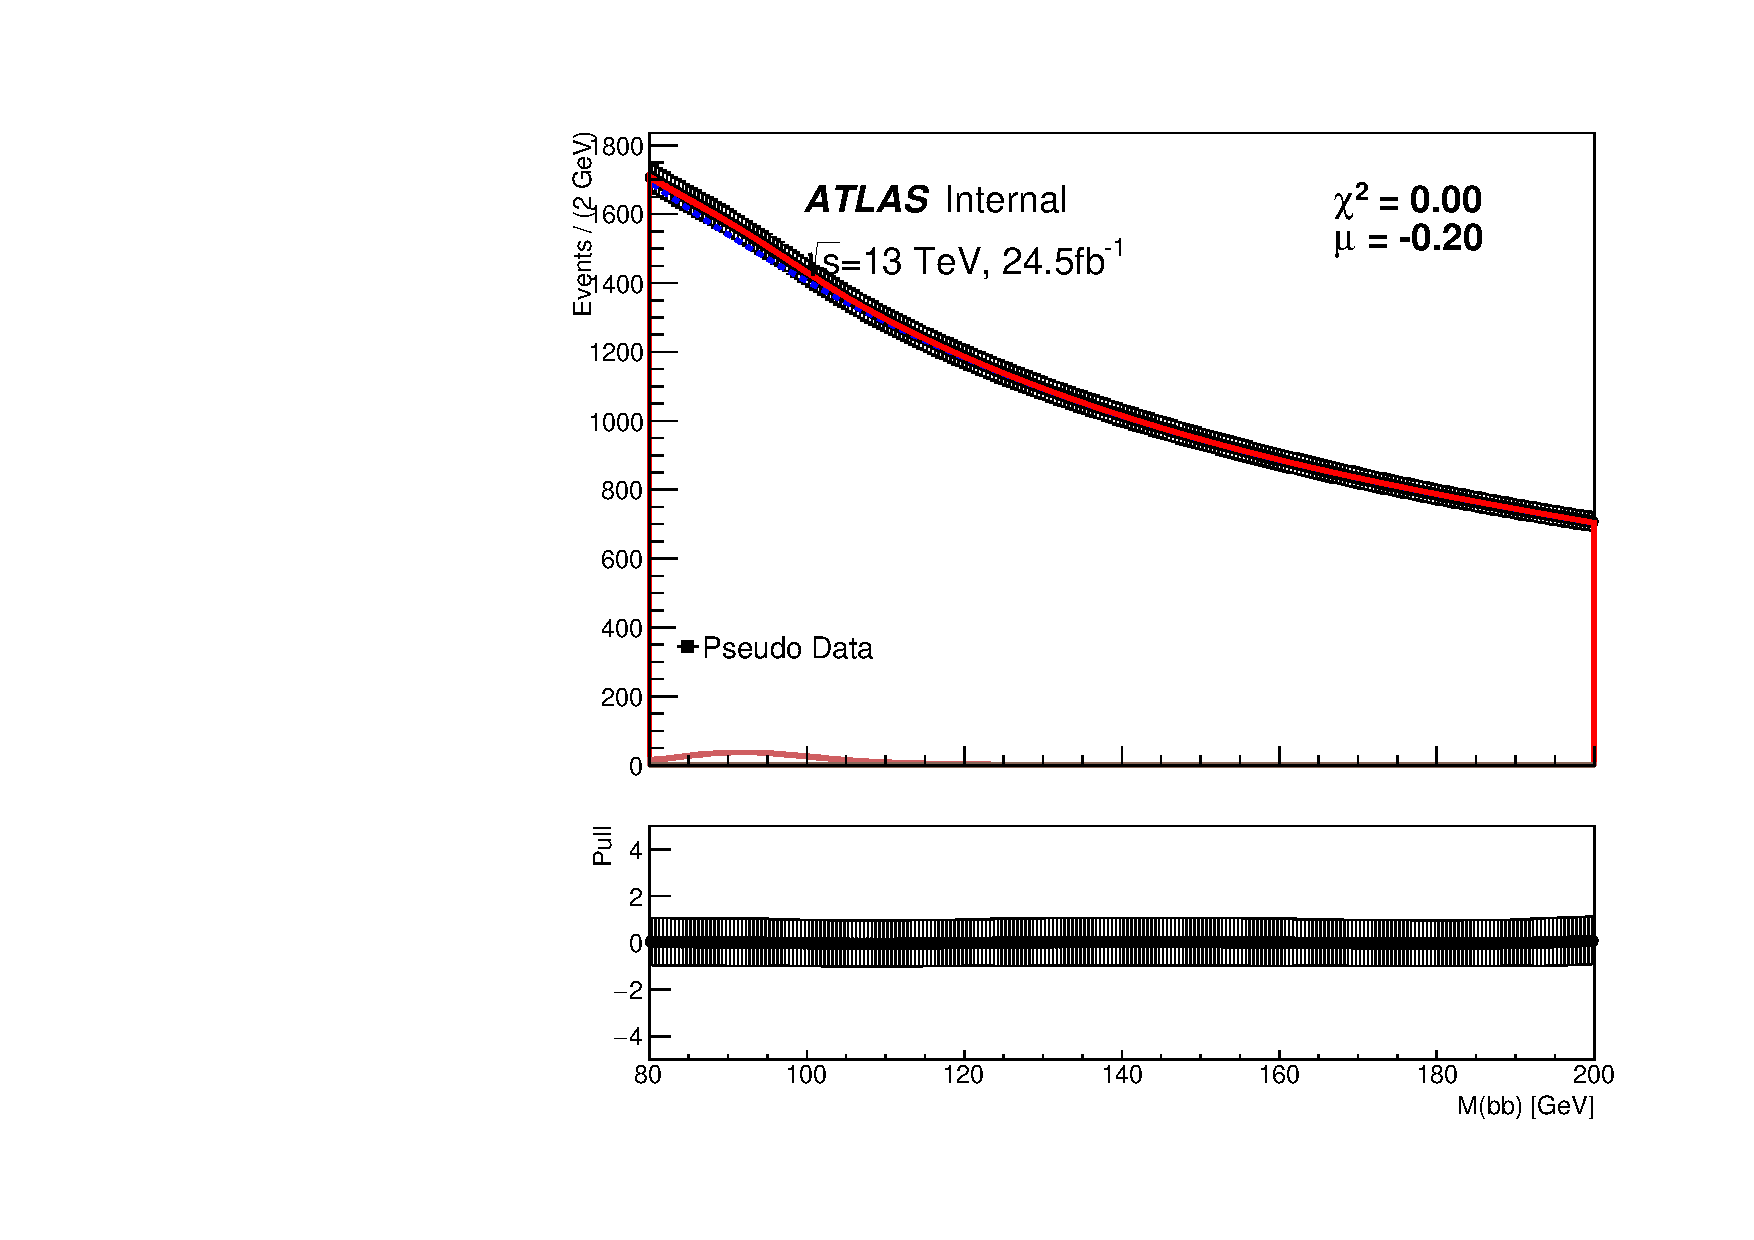
\includegraphics[width=0.24\textwidth]{figures/VBF/Spurious_SExpoO2_testVBF_ICHEP_2cen_SRII.pdf}\\
%\caption{Spurious signal fit for \twocentral channel for SR I to SR II (from left to right). The best Bernstein background models are tested against alternative truth models Expo*Bernstein O(2) (top) and Sum of Expo O(2) (bottom).}
%  \label{fig:vbf-Fit_SP_2cen}
%\end{figure}
%
%\begin{figure}[htbp]
%  \centering
% \includegraphics[width=0.24\textwidth]{figures/VBF/Spurious_ExpoO2_testVBF_ICHEP_4cen_SRI.pdf}
% \includegraphics[width=0.24\textwidth]{figures/VBF/Spurious_ExpoO2_testVBF_ICHEP_4cen_SRII.pdf}
% \includegraphics[width=0.24\textwidth]{figures/VBF/Spurious_ExpoO2_testVBF_ICHEP_4cen_SRIII.pdf}
% \includegraphics[width=0.24\textwidth]{figures/VBF/Spurious_ExpoO2_testVBF_ICHEP_4cen_SRIV.pdf}\\
% \includegraphics[width=0.24\textwidth]{figures/VBF/Spurious_SExpoO2_testVBF_ICHEP_4cen_SRI.pdf}
% \includegraphics[width=0.24\textwidth]{figures/VBF/Spurious_SExpoO2_testVBF_ICHEP_4cen_SRII.pdf}
% \includegraphics[width=0.24\textwidth]{figures/VBF/Spurious_SExpoO2_testVBF_ICHEP_4cen_SRIII.pdf}
% \includegraphics[width=0.24\textwidth]{figures/VBF/Spurious_SExpoO2_testVBF_ICHEP_4cen_SRIV.pdf}\\
%\caption{Spurious signal fit for \fourcentral channel for SR I to SR IV (from left to right). The best Bernstein background models are tested against alternative truth models Expo*Bernstein O(2) (top) and Sum of Expo O(2) (bottom).}
%  \label{fig:vbf-Fit_SP_4cen}
%\end{figure}



%\begin{table}[htbp]
%\centering
%\caption{Higgs sensitivity of each channel quantified in $\Delta \mu$ for different orders of non-resonant background function choice}
%\label{tab:perchannel_sensitivity}
%\begin{tabular}{|c|c|c|c|}
%\hline
%Channel      & Bernstein O2 & Bernstein O3 & Bernstein O4 \\ \hline
%2cen, SR I   & 2.09         & 2.67         &              \\ \hline
%2cen, SR II  & 5.50         & 8.09         &              \\ \hline
%4cen, SR I   & 2.86         & 3.60         &              \\ \hline
%4cen, SR II  & 6.44         & 9.32         & 10.07        \\ \hline
%4cen, SR III & 5.23         & 7.01         &              \\ \hline
%4cen, SR IV  & 4.20         & 5.51         & 5.89         \\ \hline
%\end{tabular}
%\end{table}


\subsection{Uncertainties}
\label{sec:vbf-uncertainties}

Several sources of systematic uncertainties,
affecting the normalization of signal and background and/or the shape of
the distributions used in this analysis, have been considered.  Individual sources of systematic 
uncertainty are considered uncorrelated. The systematic variations with less than $0.5\%$ impact 
on the yields in a particular BDT region will be ignored in the profile likelihood fit for 
that particular region. 

\subsubsection{Luminosity}
\label{sec:vbf-syst_lumi}

The integrated luminosity measurement has an uncertainty of 3.4\%. This systematic uncertainty
is applied to all physics processes estimated with MC simulated samples normalized 
to the measured integrated luminosity: \zjets{} and Higgs production. {\it Ed. Note: this will be updated after the unblinding.}

\subsubsection{Uncertainties on object definitions}
\label{sec:vbf-syst_objects}

Several uncertainties are applied to the MC simulation samples to take into account the limited knowledge of the detector and reconstruction performance.

\paragraph{Trigger efficiencies}

The per-jet online b-tagging efficiency with respect to the offline b-tagging efficiency is measured in $t\bar t$ events. 
To cover the event topology dependence, a scale factor applied to the leading b-tagged jet is derived as a function of the jet $\eta$. 

\paragraph{JVT efficiency}
The per-jet efficiency to satisfy the jet vertex tagging requirement
is measured in $Z(\to \ell^+\ell^-)$+1-jet events in data and simulation,
selecting separately events enriched in hard-scatter jets and events enriched in pile-up jets. 
The corresponding uncertainty is evaluated by shifting the per-jet scale factors,
accounting for the efficiency uncertainty~\cite{JVTwiki}.

\paragraph{Jet energy scale}
%\label{sec:vbf-syst_jes}
The jet energy scale and its uncertainty have been derived combining information from test-beam data, 
LHC collision data and simulation \cite{JESwiki}. The jet
energy scale uncertainty is split into 4 uncorrelated sources, 
which can have different jet $\pt$ and $\eta$ dependencies.  These sources are
treated independently in this analysis, using the \texttt{JetUncertainties} tool \cite{TWiki_JetUncertainties} 
to compute the uncertainties corresponding to each eigenvector. 
The variation in the jet energies as a result of these systematic uncertainties are also propagated through all
observables computed using jet kinematics.

\paragraph{Jet energy resolution}
%\label{sec:vbf-syst_jer}
[The jet energy resolution (JER) has been measured separately for data and simulation 
using in-situ techniques. The \texttt{JERUncertaintyProvider}
tool~\cite{jeruncertaintyprovider} was used to obtain the expected fractional
$p_T$ resolution for a given jet as a function of its $p_T$ and rapidity. 
The systematic uncertainty is taken by smearing the jet energy by the shift 
in resolution provided by the tool and comparing to the nominal
shape and normalization in simulation. 
The nominal value is used as the default in the analysis.

In order to propagate the uncertainty in the $p_T$ resolution, for each jet a 
random number $r$ is drawn from a Gaussian distribution with mean 0 and sigma equal 
 to the difference in quadrature between the fractional $p_T$ resolution with the tool and the nominal
one.  The jet 4-momentum is then scaled by a factor $1+r$.  By definition, such uncertainty
is one-sided, since jets in simulation cannot be under-smeared. 
We compute the normalization and shape uncertainties in the final distributions 
and symmetrize them to define a corresponding "down'' variation.

\paragraph{\btagging}
%\label{sec:vbf-syst_btag}

The effects of uncertainties in efficiencies for the heavy flavor tagging of jets by
the MV2c10 tagger have been evaluated. This analysis uses the operating points 
with approximately 60\%, 70\% and 85\% efficiency for $b$-quark jets. 
These efficiencies are measured
from data for each jet flavor.

Simulation efficiencies for $b$ and $c$ quarks have to be corrected by a
$\pt$-dependent factor. In the case of light flavor jets, the corrections also 
depend on jet $\eta$. 
Each uncertainty corresponds to a resulting eigenvector after diagonalizing the matrix
containing the information of total uncertainty per $\pt$ bin and the bin-to-bin 
corrections. These systematic
uncertainties are taken as uncorrelated between $b$, $c$, and light flavor jets.
A per-jet weighting procedure is applied to simulated events to propagate the 
calibration of $b$-tagging and the related uncertainties. 
The correlation across operating points is ignored. It has been checked that this choice
wouldn't impact the results by considering the uncertainties fully correlated or fully uncorrelated.


\paragraph{Track multiplicity for Quark/gluon separation}

The track multipicity discrimination power for quark/gluon separation in simulation 
is affected by the modeling of the charged multiplicity in jet fragmentation and the modeling of the
track multiplicity reconstruction. The estimation of the corresponding uncertainties is 
described in Ref.~\cite{qgtagging}. A total of 5 nuisance parameters is used to parametrize these
uncertainties and the impact on the results presented in this note is found to be negligible.

\subsubsection{Analytical and Theoretical Modeling uncertainties of signal}
\label{sec:vbf-syst_model}

Uncertainties in the modeling both of the non-resonant background shape and the theory and phenomenological modeling uncertainties of the Monte Carlo simulation samples are described here.


\paragraph{Non-resonant background}
The non-resonant background is modeled with an analytical function, either O(3) or O(4) Bernstein polynomial. 
The potential local bump or dip caused by the functional choice is characterized by spurious signal 
which is derived by fitting the nominal model plus signal to an alternative model. The derived spurious signal 
size is then quoted the width of a gaussian constraint which is included in the profile likelihood as in 
Eq.~\ref{likelihood}.

%\paragraph{\zjets{} normalization}
%\label{sec:vbf-zjets}
%
%Strategy~\label{item:z-treat-5} of section~\ref{sec:vbf-ztreat} is taken for the systematic uncertainties on the \zjets{} normalization.
%
%The bias on the signal $\mu$ value caused by this rescaling (or lack thereof) is estimated 
%with an injection test where the scaled pseudodata is fit with the non-scaled template. 
%The bias is found to be less than $10\%$ and therefore negligible with respect to the overall uncertainty.
%Therefore no relative rescaling is applied to the \zjets{} MC prediction in each region.
%Additional details of these studies are provided in Appendix ~\ref{sec:vbf-app-zmm}.

%The normalization of the \zjets{} background, simulated at LO, is 
%affected by potentially large uncertainties~\cite{zkfactors}. 
%In order to estimate the \zjets{} normalization in data, the $Z(\mu\mu)+$jets yield
%is used as proxy. The ratio between data and MC yield after preselection is used to estimate the overall
%normalization and the difference between \zjets{} and $Z(\mu\mu)+$jets is 
%taken as uncertainty.
%The data/MC ratio is found to be 0.74(0.1) and 0.79(0.1) for \twocentral and \fourcentral channels respectively. 
%A single gaussian NP with width 0.1 is therefore used in the global fit. 
%The $Z(\mu\mu)+$jets sample is also used to study the variation across signal and control regions.
%The \zjets{} prediction is scaled in each BDT region by the ratios between the yields observed in $Z(\mu\mu)+$jets data
%and in \zjets{} and $Z(\mu\mu)+$jets MC. The scale factors are listed in Table~\ref{tab:z_ratios}
% 

\paragraph{QCD Scale Variations}

The QCD scale uncertainty for VBF is taken as varying the renormalization
and factorization scales together by a factor of 2 and 0.5. As indicated in ~\cite{QCDscale_vbf}, 
this treatment in general leads to larger variations than the independent variation of renormalization
and factorization scales. 

The QCD scale uncertainty for ggF follows the \textit{2017 scheme} recommended by 
WG1 in the follow-up of March meeting 2017 ~\cite{QCDscale_ggF}. In total, nine independent 
variations in six categories are considered. The terms and corersponding uncertainty sources 
are the following:

\begin{enumerate}
\item \textit{mu}, factorization scale variation
\item \textit{res}, renormalization scale variation
\item \textit{vbf2j} and \textit{vbf3j}, VBF topology uncertainties
\item \textit{mig01} and \textit{mig12}, truth level bin migration for non-Higgs jets
\item \textit{pTH60} and \textit{pTH120}, uncertainties extrapolation with Higgs $p_T$
\item \textit{qmt}, uncertainties of top quark mass
\end{enumerate}

The dominant source of uncertainty for this analysis comes from the term \textit{mig12} (size of $~17-18\%$), 
which is the leading source of uncertainty in high $p_T(H)$ event topology. 

Naively, one would assume uncertainties due to VBF topology terms are considerable. 
However, it is worth noting that these terms only matter for events which 
at truth level are generated in VBF topology. An event falls into Stage one classification 
of VBF topology if the truth Higgs has $p_T<200GeV$ and 
\begin{enumerate}
\item $MJJ>400 GeV$ and $|\textnormal{rapidity(J1)-rapidity(J2)}|>2.8$ ( loose VBF, events having >3 jets),
\item Pass loose VBF selection $\overrightarrow{p_{T}}(J1)+\overrightarrow{p_{T}}(J2)+\overrightarrow{p_{T}}(Higgs)<25GeV$ (tight VBF, events having ~2 jets),
\end{enumerate}
where the VBF jets are defined as the leading two jets aside from the Higgs. We note that $80\%$ of the events have $p_T(H)>200GeV$ and 
these events would not fall into the VBF category. Hence, the VBF topology uncertainties would not even apply in the \textit{2017 scheme} for most of our events. 
For our application, we could extend the definition of VBF topology to high $p_T(H)$ events and take the \textit{vbf2j} and \textit{vbf3j} values
for low $p_T(H)$ VBF topology to be the uncertainty for high $p_T(H)$ events as well. (\textit{vbf2j} and \textit{vbf3j} are defined as constants.)

We also notice that the \textit{2017 scheme} has a different definition of VBF jets, which selects the leading two jets aside from Higgs,  from the 
offline selection we apply in this analysis, which seeks a pair of jets that maximizes the $MJJ$ value. Hence if an event which is categorized by \textit{2017 scheme}
as non-VBF, the scheme lacks a term to properly count the 2J VS. 3J truth event topology uncertainty. Therefore, we also propagate the VBF topology 2J VS. 3J
uncertainties to standard non-VBF ggF+GE2j category. 

Overall, if VBF topology uncertainties are only applied to low $p_T(H)$ events, this source 
of ucnertainty is $<3\%$ in all signal regions. If the uncertainty is extended to high $p_T(H)$ events and as well as non-VBF ggF+GE2j events, the uncertainty
is about $20\%$. We take this conservative extended version of uncertainty for ggF events.

%\begin{table}[htbp]
%\centering
%\caption{Fraction of ggF events in high $p_T(H)$ and VBF topology category}
%\label{tab:highpTfraction}
%\begin{tabular}{|l|l|l|l|l|l|l|}
%Region   & 2cen SR I & 2cen SR II & 4cen SR I & 4cen SR II & 4cen SR III & 4cen SR IV \\
%Fraction & 17.5\%    & 10.4\%     & 13.2\%    & 19.4\%     & 8.8\%       & 9.5\%     
%\end{tabular}
%\end{table}


\paragraph{PDF}
The uncertainty on the PDF description used to simulate the signal is evaluated
by varying the PDF based on the uncertainties along each of the PDF eigenvectors.
Each variation is applied by reweighting the signal samples event-by-event.
A single nuisance parameter, corresponding to the envelope of all the variations,
is considered.

\paragraph{Parton Shower}

The modeling of parton shower could directly affect observables which are heavily 
correlated with the jettiness of the event. In this analysis, its impact is most 
prominent on $p_{T}$ balance, which is a variable used as the BDT input. The nominal
Pythia sample is compared with the \herwig{} sample at the truth level to derive a 
reweighting map for $p_{T}$ balance.
This reweighting map is then applied to the observable of the reconstructed events. The full impact of this variation 
is evaluated by running the BDT analysis while fixing other variables at their nominal 
and applying reweighting of $p_{T}$ balance. 


\paragraph{Signal Contamination from \VH and \ttH Processes}

The cross section of other Higgs production mode like \VH and \ttH are comparable to
the VBF process. Events from \VH (fully hadronic final states) and \ttH production could 
also pass the event selections of this analysis. The \Mbb distributions of these process
 are shown in Figure~\ref{fig:Mbb-ttH-VH}. The yields of these processes are presented 
in Table~\ref{tab:vh-tth-yield}.  The contributions to the total Higgs yields are  small 
in the most sensitive signal regions (0.2 -- 0.8 \%),  and rise to 15\% in the least sensitive regions.  

The VH process has a prominent resonance peak, similar to the VBF and ggF distributions. However, 
the statistics of the Monte Carlo sample is low, especially in \twocentral channel. 
We assign a 100\% uncertainty to the \VH process yield for a conservative estimate of 
the \VH contribution. %Its yield is added to the Higgs yields from VBF and ggF processes.

The \ttH mass distribution is a combination of the resonance peak and a continuum. 
The continuum arises from the fact that the \ttH process has at least four $b$-jets in the final state.
The failure of the jet assignment to identify the correct Higgs daughter $b$-jets results in a 
continuum combinatorial background which can be clearly seen in Figure~\ref{fig:Mbb-ttH-VH}. 
The yield is also assigned with 100\% uncertainty.
%In the fit, we take the actual shape of \ttH treating it as a background. 


\begin{figure}[htbp]
  \centering
 \includegraphics[width=0.42\textwidth]{figures/VBF/Mbb_VH_2cen.pdf}
 \includegraphics[width=0.42\textwidth]{figures/VBF/Mbb_ttH_2cen.pdf}\\
 \includegraphics[width=0.42\textwidth]{figures/VBF/Mbb_VH_4cen.pdf}
 \includegraphics[width=0.42\textwidth]{figures/VBF/Mbb_ttH_4cen.pdf}
 \caption{\Mbb distributions of \VH (left) and \ttH (right) for \twocentral (top) and \fourcentral (bottom) channels passing event pre-selection. }
  \label{fig:Mbb-ttH-VH}
\end{figure}

\begin{table}[htbp]
\centering
\caption{Yields of \VH and \ttH}
\label{tab:vh-tth-yield}
\begin{tabular}{|l|l|l|l|l|}
\hline
     & \multicolumn{2}{l|}{\twocentral SR I}    & \multicolumn{2}{l|}{\twocentral SR II}  \\ \hline
     & Expected Yied  & Fraction of Total Yield & Expected Yied & Fraction of Total Yield \\ \hline
\VH  & 0.2           & 0.2\%                  & 9.3          & 6.8\%                  \\ \hline
\ttH & 4.2           & 2.9\%                  & 30.0         & 19.7\%                 \\ \hline
     & \multicolumn{2}{l|}{\fourcentral SR I}   & \multicolumn{2}{l|}{\fourcentral SR II} \\ \hline
     & Expected Yied  & Fraction of Total Yield & Expected Yied & Fraction of Total Yield \\ \hline
\VH  & 1.4           & 2.0\%                  & 0.7          & 1.4\%                  \\ \hline
\ttH & 0.6           & 0.8\%                  & 2.2          & 4.2\%                  \\ \hline
     & \multicolumn{2}{l|}{\fourcentral SR III} & \multicolumn{2}{l|}{\fourcentral SR IV} \\ \hline
     & Expected Yied  & Fraction of Total Yield & Expected Yied & Fraction of Total Yield \\ \hline
\VH  & 6.0           & 5.2\%                  & 34.1         & 13.5\%                  \\ \hline
\ttH & 12.4          & 10.2\%                 & 42.4         & 15.5\%                 \\ \hline
\end{tabular}
\end{table}

\clearpage

\subsubsection{Summary}
The typical signal yield changes due to a few representative systematic uncertainties are 
shown in Tables. \ref{tab:syst-2cen} and \ref{tab:syst-4cen}.  The theory uncertainties, especially from the QCD scale dominate, at the 20\% level across all signal regions.  The largest experimental uncertainties are from \btagging, at the 3--4\% level.

\begin{table}[hbpt]
\centering
\scriptsize
\begin{tabular}{|l|l|l|l|l|l|l|}
\hline
                 & \multicolumn{6}{c|}{\twocentral}                     \\ \hline
                 & \multicolumn{3}{c|}{SRI} & \multicolumn{3}{c|}{SRII} \\ \hline
                 & Total  & VBF    & ggF    & Total   & VBF    & ggF    \\ \hline
Jet Energy Scale NP1           & 0.75   & 1.19   & 1.14   & 2.54    & 4.11   & 2.07   \\ \hline
Jet Energy Scale \bjets        & 1.52   & 1.62   & 1.08   & 2.21    & 2.71   & 2.06   \\ \hline
Jet Energy Resolution          & 1.65   & 3.03   & 4.11   & 2.16    & 4.69   & 4.19   \\ \hline
\qgtagging                     & 0.65   & 0.73   & 0.28   & 1.39    & 2.12   & 1.18   \\ \hline
Pile-up Reweighting            & 0.49   & 0.18   & 1.74   & 0.18    & 0.99   & 0.54   \\ \hline
\btagging NP0 70WP             & 2.66   & 2.67   & 2.60   & 2.88    & 2.74   & 2.92   \\ \hline
\btagging NP0 85WP             & 0.80   & 0.87   & 0.52   & 1.26    & 1.08   & 1.31   \\ \hline
$\alpha_s$                     & 0.73   & 0.14   & 3.18   & 2.66    & 3.95   & 3.35   \\ \hline
QCD scale VBF                  & 9.92   & 12.29  & 0      & 2.41    & 10.50  & 0      \\ \hline
QCD scale ggF                  & 8.17   & 0      & 42.33  & 29.61   & 0      & 41.91  \\ \hline
PDF Variations                 & 10.08  & 11.52  & 4.16   & 6.36    & 9.56   & 5.42   \\ \hline
Parton Shower                  & 0.34   & 1.06   & 2.69   & 0.62    & 1.92   & 0.24   \\ \hline
\end{tabular}
\caption{Yield change in percentage due to $\pm 1 \sigma$ variation of systematics for \twocentral for combined signal, VBF and ggF production modes. }
\label{tab:syst-2cen}
\end{table}


\begin{table}[hbpt]
\centering
\scriptsize
\begin{tabular}{|l|l|l|l|l|l|l|l|l|l|l|l|l|}
\hline
                    & \multicolumn{12}{c|}{\fourcentral}                                                                                \\ \hline
                    & \multicolumn{3}{c|}{SR I} & \multicolumn{3}{c|}{SR II} & \multicolumn{3}{c|}{SR III} & \multicolumn{3}{c|}{SR IV} \\ \hline
                    & Total   & VBF    & ggF    & Total   & VBF     & ggF    & Total   & VBF     & ggF     & Total   & VBF     & ggF    \\ \hline
Jet Energy Scale NP1      & 3.38    & 1.05   & 18.50  & 0.65    & 0.57    & 3.10   & 1.56    & 2.43    & 0.76    & 1.12    & 0.59    & 1.44   \\ \hline
Jet Energy Scale \bjets   & 0.21    & 0.64   & 1.67   & 1.48    & 1.57    & 12.9   & 0.49    & 1.35    & 0.31    & 1.66    & 2.25    & 1.46   \\ \hline
Jet Energy Resolution     & 1.16    & 1.25   & 12.04  & 0.35    & 2.20    & 3.38   & 3.96    & 1.14    & 8.64    & 1.13    & 0.79    & 1.78   \\ \hline
\qgtagging                & 3.98    & 2.41   & 10.69  & 0.21    & 0.60    & 1.86   & 0.33    & 1.81    & 0.22    & 0.11    & 4.27    & 1.56   \\ \hline
Pile-up Reweighting       & 0.34    & 0.38   & 0.17   & 2.17    & 2.06    & 4.19   & 1.49    & 0.19    & 3.04    & 2.55    & 2.23    & 2.66   \\ \hline
\btagging NP0 77WP        & 4.37    & 4.33   & 4.53   & 4.19    & 4.17    & 4.23   & 4.30    & 4.12    & 4.47    & 4.21    & 4.15    & 4.25   \\ \hline
$\alpha_s$                & 0.76    & 0.16   & 3.35   & 1.32    & 0.23    & 3.45   & 1.85    & 0.34    & 3.23    & 2.85    & 0.90    & 3.49   \\ \hline
QCD scale VBF             & 6.69    & 8.25   & 0      & 5.39    & 8.06    & 0      & 3.86    & 8.08    & 0       & 1.98    & 7.95    & 0      \\ \hline
QCD scale ggF             & 7.83    & 0      & 41.56  & 12.86   & 0       & 40.66  & 22.67   & 0       & 43.42   & 31.99   & 0       & 42.60  \\ \hline
PDF Variations            & 6.19    & 6.44   & 5.16   & 5.62    & 6.33    & 4.18   & 5.03    & 6.11    & 4.05    & 4.95    & 7.23    & 4.19   \\ \hline
Parton Shower             & 3.24    & 4.14   & 0.62   & 1.75    & 3.56    & 1.87   & 2.36    & 0.31    & 0.96    & 0.26    & 0.32    & 0.24   \\ \hline
\end{tabular}
\caption{Yield change in percentage due to $\pm 1 \sigma$ variation of systematics for \fourcentral for combined signal, VBF and ggF production modes.}
\label{tab:syst-4cen}

\end{table}


\subsection{Binned Likelihood Maximization}
\label{sec:vbf-likelihood}

\subsubsection{Yield and likelihood}
The negative log-likelihood is constructed as shown in Equation~\ref{likelihood}, 
where $Y_{ijk}$ denotes the yield of $k^{th}$ bin of $j^{th}$ region of $i^{th}$ channel. 
Nuisance parameters, which have external constraints $f(\alpha_l)$, are penalized in the negative log-likelihood. 

Both \twocentral{} and  \fourcentral{} channel consists of four signal regions and yield in total eight \Mbb{} distributions.
The yield of a given region R is calculated with Equation~\ref{yield_float}. Note in the equation that a Gaussian constraint $\alpha_{sp}$  for spurious signal is included with width being the spurious signal size we measured in the spurious signal test.

Free parameters are the normalizations of the non-resonant background in each control and
signal region, denoted with $N_B$.
The signal normalizations $N_H$ are set to the Standard Model expectation from simulation,
while $\mu$ represents the observed signal strength.
The shapes of Higgs, Z and non-resonant background are $H$, $Z$ and $B$, respectively.

\begin{equation}
\label{likelihood}
-\log\mathcal{L}(\mu, \{\alpha_{l}\} )= -\log \prod_{i=1}^{\textnormal{Channels}} \prod_{j=1}^{\textnormal{Regions}} \prod_{k=1}^{\textnormal{Bins}} \frac{e^{-Y_{ijk}(\mu, \{\alpha_l\})} \times Y_{ijk}N_{ijk}^{Obs} }{N_{ijk}^{Obs}} - \log \prod_{l}^{\textnormal{Nuisance Pars}} f(\alpha_l)
\end{equation}

\begin{equation}
\label{yield_float}
\begin{split}
Y(R) &= (\mu + \alpha_{sp}(R))N_{H}H(R)+ N_{B}B(R)+ \mu_{z}(R)N_{Z}Z  \\
\end{split}
\end{equation}


Eq.\ref{yield_float} adopts the strategy floating the $Z$ contributions in all BDT regions. 


%In case we adopt the method only floating the $Z$ contributions in SR I and SR II of \twocentral, the rest of the regions will have yield as in Eq.\ref{yield_constrain} where $\mu_z(Norm)$ stands for the floating parameters for $Z$ normalization and $\alpha_z(R)$ stands for the BDT shape nuisance parameter with 50\% width. 

%\begin{equation}
%\label{yield_constrain}
%\begin{split}
%Y(R) &= (\mu + \alpha_{sp}(R))N_{H}H(R)+ N_{B}B(R)+ \mu_{z}(Norm)\alpha_z(R)N_{Z}Z  \\
%\end{split}
%\end{equation}



%The nuisance parameter $\alpha_{z}$ controls the overall normalization for the \zjets{} template 
%and is constrained with a Gaussian prior with width 0.06. The overall normalization is scaled
% to 0.81 and 0.75 for \twocentral and \fourcentral channels, respectively, determined as described in Section~\ref{sec:vbf-ztreat}..
%We also adopt independent NPs for each BDT region to account the data/MC shape difference of \zjets{}. 
%The chosen values are motivated by the validation study in data described in Appendix~\ref{sec:vbf-zjets}. 


\subsubsection{Fits on toy experiments}

To determine if the fit procedure yields bias, we build 2000 toy experiments from the background function determined in background only fit and inject the \zjets{} component fixed at the Standard Model prediction. The Higgs signals are injected of different strengths at $\mu_{inj} = 0.5, 1.0, 2.0, 5.0$. The pulls of the toy experiment fits defined as $(\mu_{fit}-\mu_{inj})/ \sigma$ are shown in Figures \ref{fig:MCToy}. The distributions of pulls are fitted with Gaussian distribution to determine means and widths, which are consistent with 0 and 1, respectively, within statistical uncertainties. For $\mu_{inj}=1.0$ test, we fit back $\hat{\mu}=1.0\pm 1.9$. %treating all NPs except the analytical background parameterization and normalization as systeamtics. 
The expected signal significance in this case is 0.5. The dominant uncertainty is statistical which encompasses the normalization and parameterization of the non-resonant background. The Z signal strength is shown in Table \ref{tab:zstrength}. The effective combined Z signal strength is $1.0\pm 0.1$. %(If we adopt the strategy to only float the $Z$ contribution in SR I and SR II of \twocentral channel, we get $\hat{\mu}=1.00\pm 1.35$). 

\begin{figure}[htbp]
  \centering
 \includegraphics[width=0.45\textwidth]{figures/VBF/Mu05.pdf}
 \includegraphics[width=0.45\textwidth]{figures/VBF/Mu1.pdf}\\
 \includegraphics[width=0.45\textwidth]{figures/VBF/Mu2.pdf}
 \includegraphics[width=0.45\textwidth]{figures/VBF/Mu5.pdf}\\
\caption{Pull distribution of toy experiment fits. We inject Higgs signal strength of 0.5 (top left), 1.0 (top right), 2.0 (bottom left) and 5.0 (bottom right) times the Standard Model prediction. The pulls are fitted with Gaussian to determine the means and widths which are unbiased. }
  \label{fig:MCToy}
\end{figure}

\begin{table}[htbp]
\centering
\caption{Floating Z normalization parameters in Asimov fit}
\label{tab:zstrength}
\begin{tabular}{|c|c|}
\hline
Region               & Asimov fit Z signal strength \\ \hline
SR I, \twocentral    & $ 1.00 \pm 0.7$              \\ \hline
SR II, \twocentral   & $ 1.00 \pm 0.5$             \\ \hline
SR I, \fourcentral   & $ 1.00 \pm 1.1$             \\ \hline
SR II, \fourcentral  & $ 1.00 \pm 0.6$             \\ \hline
SR III, \fourcentral & $ 1.00 \pm 0.3$             \\ \hline
SR IV, \fourcentral  & $ 1.00 \pm 0.2$             \\ \hline
\end{tabular}
\end{table}



%The uncertainties and pulls in the fit are shown in Figure~\ref{fig:pull_asimov} and the correlation matrix is shown in Figure~\ref{fig:corr_asimov}.
The fit correlation matrix is shown in Figure~\ref{fig:corr_asimov}. We observe, as expected, the Higgs signal is mildly anti-correlated with background normalization, Z strength and spurious signal size. The Z signal strength also shows as expected to be anti-correlated to background normalization given the degeneracy between the Z mass region and the low-mass sideband. The background parameters within a given channel are highly correlated as the variation of the contribution of one base function will need the variation of other bases to maintain the same background shape. 


%\begin{figure}[htbp]
%  \centering
% \includegraphics[width=0.48\textwidth]{figures/VBF/Asimov_testVBF_ICHEP_2cen_SRI.pdf}
% \includegraphics[width=0.48\textwidth]{figures/VBF/Asimov_testVBF_ICHEP_2cen_SRII.pdf}\\
%\caption{Asymptotic Asimov fits for SRI and SRII for the \twocentral channel.}
%  \label{fig:2cenAsimov}
%\end{figure}
%
%\begin{figure}[htbp]
%  \centering
% \includegraphics[width=0.48\textwidth]{figures/VBF/Asimov_testVBF_ICHEP_4cen_SRI.pdf}
% \includegraphics[width=0.48\textwidth]{figures/VBF/Asimov_testVBF_ICHEP_4cen_SRII.pdf}
% \includegraphics[width=0.48\textwidth]{figures/VBF/Asimov_testVBF_ICHEP_4cen_SRIII.pdf}
% \includegraphics[width=0.48\textwidth]{figures/VBF/Asimov_testVBF_ICHEP_4cen_SRIV.pdf}\\
%
%\caption{Asymptotic Asimov fits for SRI to SRIV for the \fourcentral channel.}
%  \label{fig:4cenAsimov}
%\end{figure}


%\begin{figure}[htbp]
%  \centering
% \includegraphics[width=0.9\textwidth]{figures/VBF/VBFHbb_Asimov_pulls_125.pdf}
% \caption{Nuisance parameter post-fit impact ($>1$ \%) and pulls are plotted for the simultaneous Asimov fit. Only the constrained NPs are shown. The uncertainties follow the naming defined in Table. \ref{tab:systnames}. The leading systematics are the jet energy scale and jet energy resolution}
%  \label{fig:pull_asimov}
%\end{figure}


\begin{figure}[htbp]
  \centering
 \includegraphics[width=0.8\textwidth]{figures/VBF/Correlation.pdf}

\caption{Nuisance parameter correlation for Asimov fit. Only parameters with $>0.2$ correlations are shown. The background normalizations are pre-fixed as ``nbkg''. The spurious signal size are pre-fixed as ``sp''. The background parameterizations are pre-fixed as ``a1,a2,...,a5'' as defined in \ref{eq:bernstein}. The Z floating parameters are pre-fixed as ``sf\_z''. }
  \label{fig:corr_asimov}
\end{figure}





\clearpage

\section{Results}
\subsection{VBF \Hbb Unblinded Results}
The VBF \Hbb analysis unblinding proceeds in two steps. First, overall strategy is validated with a fit to the $Z$ contribution in a sideband only fit while the Higgs mass window is kept unblinded, shown in Section~\ref{sec:vbf-zunblind}.  Then a simultaneous fit to the signal, correlated over all signal regions, and the $Z$ signal, uncorrelated across signal regions, is done over the entire mass region, as described in~\ref{sec:vbf-higgsunblind}. As an alternative interpretation of this analysis the $\mu_{VBF}$ strength is extracted by only allowing $VBF$ events to float in the fit and fixing all other Higgs processes, i.e. ggF, ttH and VH, to Standard Model expectation, as described in~\ref{sec:vbf-higgsunblindvbf}. The combination of inclusive $VBF$ and $VBF+\gamma$ results are presented in~\ref{sec:vbf-higgscomb}.


\subsection{Unblinding of \zjets{} in mass sidebands}
\label{sec:vbf-zunblind}

The fit strategy is first validated in data with a closure obtained in \zjets{} mass sideband fit. We performed a side-band only fit to extract the \zjets{} contribution independently in all regions. The fitted \zjets{} strengths are summarized in Table~\ref{tab:zsidebandfit}, presented with with all experimental and statistical uncertainties.   Note that we have no BDT shape uncertainties on the \zjets{} MC so cannot draw any conclusions from the compatibility of $\mu_Z$ with 1 in the different BDT regions. The effective $\mu_{Z}^{\rm eff}$ of all regions combined is defined as
\begin{equation}
\label{eqn:zsig}
\mu_{Z}^{\rm eff} = \sum \mu_{Z,i}\frac{n_{Z,i}}{\sum n_{Z,i}} 
\end{equation}
where $n_{Z,i}$ is the number of $Z$ events in region $i$, and $\mu_{Z,i}$ is the measured $\mu_Z$ in region $i$.  $\mu_{Z}^{\rm eff}$ is measured to be $1.0\pm 0.4$ in the sideband only fit with a compatibility of $\chi^2/nodf = 5.5/6=0.9$ ($\chi^2$ probability of 48\%).


\begin{table}[htbp]
\centering
\caption{Floating Z normalization parameters in data sideband fit including all systematic uncertainties.}
\label{tab:zsidebandfit}
\begin{tabular}{|l|c|c|}
\hline
Channel      & $\mu_{Z}$   & $\chi^2/ndof$ \\ \hline
2 cen SR I   & 2.6 $\pm$1.3  & 1.1          \\ \hline
2 cen SR II  & 0.4$\pm$0.8  & 0.7          \\ \hline
4 cen SR I   & 2.2$\pm$2.0  & 0.8          \\ \hline
4 cen SR II  & 2.0$\pm$1.9  & 0.9          \\ \hline
4 cen SR III & 1.9$\pm$0.6  & 0.9          \\ \hline
4 cen SR IV  & 0.6$\pm$0.6  & 0.9          \\ \hline
\end{tabular}
\end{table}



%\begin{figure}[htbp]
%  \centering
% \includegraphics[width=0.24\textwidth]{figures/VBF/zunblind_testVBF_ICHEP_2cen_SRI.pdf}
% \includegraphics[width=0.24\textwidth]{figures/VBF/zunblind_testVBF_ICHEP_2cen_SRII.pdf}\\
% \includegraphics[width=0.24\textwidth]{figures/VBF/zunblind_testVBF_ICHEP_4cen_SRI.pdf}
% \includegraphics[width=0.24\textwidth]{figures/VBF/zunblind_testVBF_ICHEP_4cen_SRII.pdf}
% \includegraphics[width=0.24\textwidth]{figures/VBF/zunblind_testVBF_ICHEP_4cen_SRIII.pdf}
% \includegraphics[width=0.24\textwidth]{figures/VBF/zunblind_testVBF_ICHEP_4cen_SRIV.pdf}\\
%\caption{Data and fit model comparison for sideband only \zjets{} fit in \twocentral (top) and \fourcentral channel (bottom) for SR I (left) to SR IV (right).  The data are the black points and the fit model (red), which comprises the continuum background (blue dashed line) and the Z contribution (light red histogram).}
%  \label{fig:vbf-zsidebandfit}
%\end{figure}


\subsection{Extraction of $\mu_{H}$}
\label{sec:vbf-higgsunblind}

The observed value of the Higgs signal strength is $2.7^{+2.2}_{-2.0}$, while the Asimov fit yields $\mu_{H}=1\pm 1.9$. The breakdown of the uncertainty is $\mu_H=2.7^{+1.9}_{-1.9}\textnormal{(stat)}^{+1.1}_{-0.6}\textnormal{(syst)}$ treating the NPs for the analytical background parameterization and normalization as well as the normalization of $Z$ contribution as statistical uncertainty.

%Figures~\ref{fig:vbf-higgsfit_2cen} and ~\ref{fig:vbf-higgsfit_4cen} show the resulting distributions for the \twocentral and \fourcentral channels. %displaying the residuals with respect to the continuum background fit on the bottom panel. % whereas Figures~\ref{fig:vbf-higgsfit_2cen_pull} and~\ref{fig:vbf-higgsfit_4cen_pull} show the pull values with respect to the full background model.  

%The pull values are shown in Figure~\ref{fig:vbf-higgsfitpull} for nuisance parameters with a post-fit impact of more than 4\%.  None of the nuisance parameters are strongly pulled. The largest uncertainty on $\mu_H$ comes from the theory uncertainty on the QCD scale, followed by the background parameterization and the jet energy resolution. The increase of the total uncertainty with respect to the expected value comes from the larger than expected background normalization as well as an increase of the signal systematics which scales as the size of the $\mu_H$. 

The fitted $Z$ values are shown in Table~\ref{tab:zfullfit} for each SR.  Reductions of 30--60\% of the $\mu_Z$ uncertainties are observed with respect to the sideband only fit. A statistical combination of all the channels, as described in Equation~\ref{eqn:zsig}, yields an effective $\mu_Z = 1.2 \pm 0.2$ with a combined $\chi^2/$ndof of 1.05 with a probability of 38.8\%.  

\begin{table}[htbp]
\centering
\caption{Floating Z normalization parameters in full mass range fit.}
\label{tab:zfullfit}
\begin{tabular}{|l|c|c|}
\hline
Channel      & $\mu_{Z}$   & $\chi^2/ndof$ \\ \hline
2 cen SR I   & 2.2$\pm$0.7  & 0.9      \\ \hline
2 cen SR II  & 0.4$\pm$0.4  & 0.7        \\ \hline
4 cen SR I   & 0.3$\pm$1.1  & 0.7         \\ \hline
4 cen SR II  & 1.2$\pm$0.6  & 0.7        \\ \hline
4 cen SR III & 1.4$\pm$0.4  & 0.7         \\ \hline
4 cen SR IV  & 0.9$\pm$0.2  & 0.8          \\ \hline
\end{tabular}
\end{table}


%\begin{figure}[htbp]
%  \centering
% \includegraphics[width=0.48\textwidth]{figures/VBF/unblind_testVBF_ICHEP_2cen_SRI.pdf}
% \includegraphics[width=0.48\textwidth]{figures/VBF/unblind_testVBF_ICHEP_2cen_SRII.pdf}\\
%\caption{Data and fit model comparison for profile likelihood fit in the \twocentral channel signal regions.  The fitted continuum background is shown with at  dashed green line, the fitted $Z$ signal in green, and the fitted Higgs signal in red.  The total fit is displayed as the blue line.  The bottom panels show the residual of the data with respect to the continuum background fit, and the fitted $Z$ signal (grey) and Higgs signal (red) are also displayed. }
%  \label{fig:vbf-higgsfit_2cen}
%\end{figure}
%
%\begin{figure}[htbp]
%  \centering
% \includegraphics[width=0.48\textwidth]{figures/VBF/unblind_testVBF_ICHEP_4cen_SRI.pdf}
% \includegraphics[width=0.48\textwidth]{figures/VBF/unblind_testVBF_ICHEP_4cen_SRII.pdf}\\
% \includegraphics[width=0.48\textwidth]{figures/VBF/unblind_testVBF_ICHEP_4cen_SRIII.pdf}
% \includegraphics[width=0.48\textwidth]{figures/VBF/unblind_testVBF_ICHEP_4cen_SRIV.pdf}\\
%\caption{Data and fit model comparison for profile likelihood fit in the \fourcentral channel signal regions. The fitted continuum background is shown with at  dashed green line, the fitted $Z$ signal in green, and the fitted Higgs signal in red.  The total fit is displayed as the blue line.  The bottom panels show the residual of the data with respect to the continuum background fit, and the fitted $Z$ signal (grey) and Higgs signal (red) are also displayed.}
%  \label{fig:vbf-higgsfit_4cen}
%\end{figure}


\subsection{Extraction of $\mu_{VBF}$}
\label{sec:vbf-higgsunblindvbf}
A different interpretation of the analysis is the extraction of $\mu_{VBF}$ signal strength.
The fit procedure follows the same way as the extraction of $\mu_{H}$, except we only float
the $VBF$ signal in the fit while fixing the yield of all other Higgs modes, i.e. ggF,
ttH and VH to their Standard Model predictions (with uncertainties applied).
The Asimov fit yields $\mu_{VBF}=1\pm 2.8$. The unblinded value of the VBF Higgs signal
strength is $4.1^{+3.2}_{-2.9}$. The breakdown of the uncertainty
is $\mu_{VBF}=4.1^{+2.8}_{-2.8}\textnormal{(stat)}^{+1.5}_{-0.8}\textnormal{(syst)}$ treating
the NPs for the analytical background parameterization and normalization as well as
the normalization of $Z$ contribution as statistical uncertainty.


\subsubsection{Combination with VBF$+\gamma$ Analysis}
\label{sec:vbf-higgscomb}

The combination of the all-hadronic VBF analysis and the
VBF$+\gamma$ analysis~\cite{vbfplusgammaint} is performed
by a simultaneous likelihood fit to both datasets. The Higgs signal strength is
treated as correlated across all analysis regions,
the $Z$ contributions are extracted as described in the respective analyses.
As described in Section~\ref{sec:vbf-presel}, overlap between the two samples is removed.

The combined fit yields $\mu_H = 2.5^{+1.4}_{-1.3}$ corresponding to an observed significance
of $1.9\sigma$ ($0.8\sigma$ expected). The $VBF$ signal only extraction is also performed combining two analyses similar to \ref{sec:vbf-higgsunblindvbf}. The combined fit yields $\mu_{VBF} =3.0^{+1.7}_{-1.6}$ corresponding to an observed significance of $1.9\sigma$ ($0.7\sigma$ expected). The data and fit model comparisons for $\mu_{VBF}$ extraction are shown in Fig.\ref{fig:higgsfit_2cen},\ref{fig:higgsfit_4cen},\ref{fig:mbb_postfit_photon}.

The extractions of $\mu_{H}$ and $\mu_{VBF}$ for separate fits of both all-hadronic and photon analysis and the combination fit are summarized in Fig.\ref{fig:vbf-summary}.


\begin{figure}[htbp]
  \centering
 \includegraphics[width=0.48\textwidth]{figures/VBF/comb_vbfonly_testVBF_ICHEP_2cen_SRI_vbfincl.pdf}
 \includegraphics[width=0.48\textwidth]{figures/VBF/comb_vbfonly_testVBF_ICHEP_2cen_SRII_vbfincl.pdf}\\

\caption{Data and fit model comparison for the combined fit of $\mu_{VBF}$ extraction in the \twocentral channel}
  \label{fig:higgsfit_2cen}
\end{figure}

\begin{figure}[htbp]
  \centering
  \includegraphics[width=0.48\textwidth]{figures/VBF/comb_vbfonly_testVBF_ICHEP_4cen_SRI_vbfincl.pdf}
 \includegraphics[width=0.48\textwidth]{figures/VBF/comb_vbfonly_testVBF_ICHEP_4cen_SRII_vbfincl.pdf}\\
 \includegraphics[width=0.48\textwidth]{figures/VBF/comb_vbfonly_testVBF_ICHEP_4cen_SRIII_vbfincl.pdf}
 \includegraphics[width=0.48\textwidth]{figures/VBF/comb_vbfonly_testVBF_ICHEP_4cen_SRIV_vbfincl.pdf}\\

\caption{Data and fit model comparison for the combined fit of $\mu_{VBF}$ extraction in the \fourcentral channel}
  \label{fig:higgsfit_4cen}
\end{figure}



\begin{figure}[htbp]
\centering

\includegraphics[width=0.48\textwidth]{figures/VBF/comb_vbfonly_testchannel1_vbfg.pdf}
\includegraphics[width=0.48\textwidth]{figures/VBF/comb_vbfonly_testchannel2_vbfg.pdf}
\includegraphics[width=0.48\textwidth]{figures/VBF/comb_vbfonly_testchannel3_vbfg.pdf}
\caption{Data and fit model comparison for the combined fit of $\mu_{VBF}$ extraction in the \textit{photon} channel}
\label{fig:mbb_postfit_photon}
\end{figure}


\begin{figure}[htbp]
  \centering
  \includegraphics[width=0.49\textwidth]{figures/VBF/Plot_mu_summary_VBF.pdf}
  \includegraphics[width=0.49\textwidth]{figures/VBF/Plot_mu_summary_VBFonly.pdf}

\caption{Summary of the extraction of $\mu_{H}$(left) and $\mu_{VBF}$(right) for  \textit{all-hadronic}, \textit{photon} and combination fits.}
  \label{fig:vbf-summary}
\end{figure}



%\begin{figure}[htbp]
%  \centering
% \includegraphics[width=0.8\textwidth]{figures/VBF/VBFHbb_pulls_125.pdf}
% \caption{Nuisance parameter post-fit impact and pulls are plotted for the data fit. Only the constrained NPs are shown. The uncertainties follow the naming defined in Table. \ref{tab:systnames}.}
%  \label{fig:vbf-higgsfitpull}
%\end{figure}

Regarding the treatment of uncertainties, both the inclusive and photon analyses apply systematics trimming. The inclusive analyses ignore nuisance parameters with yield impact $<0.5\%$ while the photon analysis ignore systematics with yield impact $<1\%$. Some NPs, for instance the third effective NP of jet energy scale may pass the systematics trimming cut of one analysis but not the other and therefore only show up in the combination fit for one analysis. 

Same set of nuisance parameters of detector related uncertainties including jet energy scale/resolution, luminosity, pile-up reweighting and q/g tagging is used by both analyses and hence treated as correlated.  $b$-tagging related uncertainties are an exception because the operating points are different between the two analyses. The inclusive analysis uses 70\% and 85\% WPs for \twocentral and \fourcentral channels respectively and the VBF$+\gamma$ analysis uses the 77\% WP. We experimented correlating NPs of the $b$-tagging uncertainties with highest impact, e.g. alpha\_FT\_EFF\_Eigen\_B\_0 of different WPs, across the two analyses and observed negligible change in the final result. Therefore the $b$-tagging NPs are left to be un-correlated.

Common terms of theoretical uncertainties including QCD scale of VBF process, parton shower and variation of $ttH$ yield are also correlated as the underlying variations are derived with same approaches. Background systematics such as non-resonant background normalization/parameterization, Z normalization and spurious signals are specific to each analysis and are not correlated.

The combination fit pull for $\mu_H$ is shown in Fig.\ref{fig:vbf-higgsfitpull_combination}. The combination fit pull for $\mu_{VBF}$ is shown in Fig.\ref{fig:vbf-vbffitpull_combination}. None of the systematics nuisance parameters are pulled significantly from their central values. One event display for the SRI of the \twocentral channel, the most sensitive BDT region, is shown in Fig.\ref{fig:vbf-evtdisplay}.


%%% no longer needed as VBF inclusive breaks down the QCD scale for VBF and ggF separately:  The inclusive and VBF$+\gamma$ analyses have some overlaps in the treatment of the QCD scale uncertainty although do not use exactly the same procedure therefore, by default, it is treated as uncorrelated.  The VBF$+\gamma$ analysis generates samples at truth level with changes by factors of two in the QCD scale and then does a truth-level calculation of the impact on the acceptance and normalization.  This analysis uses weights generated according to the \textit{WG1 scheme} (see Section~\ref{sec:vbf-syst_model}). Since it is a large systematic uncertainty for both analyses, we also try to correlate this particular nuisance parameter. The combined fit correlating the QCD scale uncertainty yields $\mu_H = 2.40^{+1.37}_{-1.32}$, which has a negligible difference with respect to the uncorrelated treatment. Hence we eventually adopt the result treating QCD scale as un-correlated as it is a more conservative approach. 


\begin{figure}[htbp]
  \centering
 \includegraphics[width=0.8\textwidth]{figures/VBF/VBFHbb_Combined_pulls_125.pdf}
\caption{Data fit pulls for nuisance parameters with a post-fit impact $> 2$ \% for $\mu_H$ combining VBF inclusive and VBF$+\gamma$ analyses.}
  \label{fig:vbf-higgsfitpull_combination}
\end{figure}

\begin{figure}[htbp]
  \centering
 \includegraphics[width=0.8\textwidth]{figures/VBF/VBFHbb_Combined_vbfonly_pulls_125.pdf}
\caption{Data fit pulls for nuisance parameters with a post-fit impact $> 2$ \% for $\mu_{VBF}$ combining VBF inclusive and VBF$+\gamma$ analyses.}
  \label{fig:vbf-vbffitpull_combination}
\end{figure}


\begin{figure}[htbp]
  \centering
 \includegraphics[width=0.8\textwidth]{figures/VBF/EvtDisplay2cen}
\caption{Event display of a \twocentral candidate event in SR I of the with \Mbb = 147 GeV. The cones representing the jets are colored magenta for the forward jets and orange for the b-tagged jets. The transverse momenta of the leading forward jet and sub-leading forward jet are 130.5 GeV and 82.0 GeV respectively. The pseudorapidity of the leading forward jet and sub-leading forward jet are -2.0 and 3.6 respectively}
  \label{fig:vbf-evtdisplay}
\end{figure}



\clearpage
\subsection{Higgs Combination}
\subsubsection{\Hbb combination}

In summer of 2018, \Hbb is observed at the ATLAS experiment \cite{VHPaper} confirming the Higgs to quark Yukawa coupling. Three separate \Hbb production modes: VH, ttH and VBF including both Run I and Run II data are combined for a measurement. The 7\TeV data and 8\TeV data have luminosity of $4.7\ifb$ and $20.3\ifb$ respectively. The 13\TeV analyses use data with luminosity ranging from $24.5-79.8\ifb$. This combination measured observed signal strength to be $\mu_{\Hbb}= 1.01 \pm 0.20 = 1.01 \pm 0.12\text{(stat.)}^{+0.16}_{-0.15}\text{(syst.)}$ with a $5\sigma$ significance.


\begin{figure}[htbp]
  \centering
 \includegraphics[width=0.8\textwidth]{figures/VBF/HbbComb.pdf}
 \caption{The fitted Higgs boson signal strength for the \Hbb combination. The combination includes 7\TeV, 8\TeV and 13\TeV data of VH, ttH and VBF analyses. Probability of signal strength compatibility of individual channel signal sterngths is 83\%.}
  \label{fig:vbf-combination-hbb}
\end{figure}



\subsubsection{Higgs combination}


\clearpage


%%%%%%%%%%%%%%%%%%%%%%%%%%%%%%%%%%%
%%%%%  RNN b-tagging
%%%%%%%%%%%%%%%%%%%%%%%%%%%%%%%%%%%
\chapter{Identification of $b$-quarks with RNN}
\label{chap:btagging}
\section{Introduction}
As discussed in Chapter \ref{chap:vbf}, the VBF \Hbb measurement requires identification of \bjets for both online and offline. Improvements of \btagging techniques can suppress the light and charm backgrounds and hence increase the sensitivity of \Hbb search. More importantly, improvement for online \btagging can lower the energy threshold for \bjet triggers and hence increase the efficiency of \Hbb event selections. This chapter focuses on improving the \btagging algorithm with Recurrent Neural Network (RNN). 

The most widely used and recommended \btagging algorithm within the ATLAS collaboration during the Run II LHC operation was \textit{MV2}. Briefly, the \textit{MV2} algorithm utilizes the different aspects of the $b$-hadron decay such as large impact parameters for its daughter tracks, existence of secondary vertex and so on. The algorithm is based on three low-level $b$-tagging algorithms: \textit{IP3D} (an impact parameter(IP)-based algorithms), \textit{SV1}(an inclusive secondary vertex-based algorithm), \textit{JetFitter} (a decay chain multi-vertex reconstruction algorithm)~\cite{ref:btagPaper}. The \textit{MV2} algorithm then takes the final and intermediate outputs from these baseline taggers as input and combines them through BDT~\cite{ATL-PHYS-PUB-2016-012}.

Many aspects of the \textit{MV2} algorithm can be improved despite its effectiveness. One could design better baseline algorithms or combination algorithm to improve \textit{MV2}. This thesis investigates particularly the improvement of the baseline algorithm \textit{IP3D}. This IP algorithm has the benefit that $b$-jet identification is possible even if no secondary vertex is explicitly reconstructed. The algorithm assigns per-track probabilities that a track is originated from a jet of a given flavor and take products of the marginal probabilities to estimate the likelihood. The per-track probabilities are estimated by referencing binned likelihood distributions from simulation while ignoring the potential correlations between them. This simplification is driven by a practical concern in the likelihood algorithm: accounting the correlations between tracks or the different track variables would need an estimation of the joint probabilities which have unmanageably large dimensions for binned linkelihood method.

To overcome these difficulties, the Recurrent Neural Network(RNN) is adopted. RNNs are a subclass of neural networks architectures that allow extensions to sequence-based and temporal domains (see~\cite{ref:RNNthesis} and references therein). They are typically used in natural language processing~\cite{languagemodel,DBLP:journals/corr/abs-1303-5778}, machine translation~\cite{MT,MT2}, and time-series analysis~\cite{timeseries,timeseries2}. In the case of $b$-tagging, the tracks in a $b$-jet can be treated as a variable-length sequence to recast $b$-tagging into a domain where RNNs have proven to be useful. This chapter presents the work of designing a new RNN-based \btagging algorithm called \textit{RNNIP}.

\clearpage

\section{Datasets and Object Definition}
The simulated $t\bar{t}$ and Z' production corresponding to $\sqrt{s}=$13~TeV proton-proton
collisions is used to study the tagger performance. Events are generated with the
next-to-leading order generator \powheg{}~\cite{bib:powheg} and the \textsc{CT10}~\cite{Lai:2010vv}
parton distribution functions, interfaced with \pythia{}~\cite{pythia2} for parton showing and
fragmentation. \textsc{EvtGen}~\cite{Lange:2001uf} is used to model the decays of
the $b$ and $c$-hadrons. Minimum bias interactions are generated with \textsc{Pythia8}~\cite{Pythia8}
and are overlaid on the $t\bar{t}$ events. Particles are passed through the ATLAS detector
simulation~\cite{atlas_simulation} which is based on \textsc{GEANT4}~\cite{geant}.

Event vertex, track and jet reconstructions follow exactly the same approach as described in \ref{sec:vbf-objsel}. Events are selected by requiring a reconstructed primary vertex. The anti-$k_t$ R=0.4 jets with JVT pile-up cleaning are used for this study. Moreover, tracks are required to pass quality requirements identical to those required by \textit{IP3D}: track $p_{T} > 1$ GeV, $| d_0 | <1$ mm and $| z_0 \sin \theta | <1.5$ mm, and seven or more silicon hits, with at most two silicon holes, at most one of which is in the pixel detector,

The tracks used in the $b$-tagging algorithms are associated to jets
using the angular separation $\Delta R$ between the track and the jet axis.
The $\Delta R$ requirement varies as a function of jet $\pt$,
being wide for low $\pt$ jets and narrower for high $\pt$ jets which tend to be more
collimated~\cite{ref:btagPaper}.
A similar geometric matching scheme to match jets with truth $b$-hadrons, $c$-hadrons and $\tau$-leptons
is used to label the flavor jets as $b$, $c$, light, or $\tau$ jets in simulation as described in ~\cite{ATL-PHYS-PUB-2015-022}.

A jet is considered as $b$-tagged if the output
discriminant of the tagging algorithm
is above certain threshold. Several such thresholds,
or ``working points'' (WP), are defined, in such a way as to correspond to
a average efficiency when applied to $b$-jets from a sample of
inclusive $t\bar{t}$ events. This study focuses on the tagger performance at
70\% $b$-tagging efficiency WP, which would retain the majority of the $b$-jets.
In addition, tagger performance for flat efficiency working points will also be considered,
which are $\pt$ dependent threshold for the tagger discriminant such that the \btagging efficiency
is uniform as a function of $\pt$.

\clearpage

\section{Recurrent Neural Network for \btagging}
\subsection{Limitations of \textit{IP3D} Algorithm}

The $b$-hadron decay gives birth to a number of charged particles with large impact parameters emerging from the same secondary vertex. Given they have the same origin, these track impact parameters are correlated. Given the jet is a $b$-jet and there is a track with large impact parameter, the probability of finding some other high impact parameter tracks in the jet is high, while the light-jet track impact parameters shall be independent. The 2D distribution of transverse impact parameter significance (\sdip) for the leading and sub-leading $|\sdip|$ tracks are shown in Figure~\ref{fig:ip_corr} for $b$-jets, where a correlation can clearly be seen, and light flavor-jets, where no such correlation is observed.

\begin{figure}[htbp]
  \centering
   \includegraphics[width=0.48\textwidth]{figures/RNN/Sd0_2d_B.pdf}
 \includegraphics[width=0.48\textwidth]{figures/RNN/Sd0_2d_L.pdf}
\caption{The distribution of the \sdip for the leading and sub-leading $|\sdip|$ significance track in $b$-jets (left) and light jets (right). }
  \label{fig:ip_corr}
\end{figure}


The baseline \textit{IP3D} $b$-tagging algorithm, uses 3D likelihood templates in $\sdip$, $\szip$, and a track categorization to compute three per-flavor conditional likelihoods, $p_b$, $p_c$, and $p_{\textrm{light}}$. These likelihood templates are derived from histograms with 35 bins in $\sdip$, 20 bins in $\szip$, and 14 bins in track category, where each category corresponds to a different track quality~\cite{ATL-PHYS-PUB-2015-022}. Direct estimate of the joint probability distribution of these three variables is not possible, as the joint distribution has a total bin count of $35 \times 20 \times 14 \times 3 = 29,400$ if we want to maintain the same resolution as for the marginal distribution of each variable.In addition, extending the template to account for additional kinematic variables and the variable number of tracks within the jet is even more computationally expensive, as the number of template bins grows exponentially.

To overcome this difficulty, the \textit{IP3D} algorithm made the assumption that is that the per-track flavor conditional likelihood can be computed independent of the other tracks in the jet.  Such a likelihood model does not take into account correlations among track parameters, and the method of building templates to define likelihoods requires large sample sizes. Technically, the \textit{IP3D} algorithm adopts a Naive Bayes estimate was made, the likelihood of a jet being of a given flavor is computed as the product of the per-track likelihoods which are in turn estimated by the product of per-track per-variable likelihoods . The \textit{IP3D} discriminant is built from the conditional log-likelihood ratio, $\textrm{IP3D}=\ln \prod_{i \in \textrm{tracks}} p_b^i / p_{\textrm{light}}^i$. 

\subsection{Recurrent Networks}

Recurrent Neural Networks are used to learn patterns in variable-length ordered inputs features~\cite{ref:RNNthesis, dlbook}. In contrast to regular multi-layer perceptrons, the forward pass equation of the hidden RNN units has in addition an activation from itself from the previous time-stamp: $O^t_l = A( W_i x_t + W_{l,l'} O^{t-1}_{l'})$, where $O$ is the output of the $l^{\text{th}}$ hidden layer's $t^{\text{th}}$ time-stamp; $A$ is the activation function, usually in the form of sigmoid function, tanh and etc.; $W_i$ are the network input weights, which is common to multi-layer perceptrons; $W_{l,l'}$ are the recurrent weights which are unique to RNNs. In this way a recurrent cell is able to reduce a sequence of arbitrary length to a fixed number of variables, which can then be processed by a traditional feed-forward network. The cell level illustration for a one-layer RNN is shown in Fig.\ref{fig:rnn_ilustration}.

\begin{figure}[htbp]
  \centering
   \includegraphics[width=0.5\textwidth]{figures/RNN/RNNIlustration.png}
\caption{Cell level illustration for a one-layer unrolled RNN}
  \label{fig:rnn_ilustration}
\end{figure}


%The fundamental unit of an RNN is a cell encapsulating an internal state vector. As the first step of processing any given sequence (in this case the tracks in a jet), the internal state is initialized to zero. At each step in the sequence, the cell is handed a fixed number of inputs (in this case the parameters that describe one track). These parameters are combined with the \emph{current} internal state in order to compute a \emph{new} internal state based on a set of rules which are tuned in the training phase. At the end of the sequence the cell's internal state serves as a fixed-dimensional representation of the entire sequence. 

It is not difficult to notice that, given a long input sequence, the derivative of the loss function with respect to the RNN weights will involve multiplicative terms which are the weights to the order of the length of the input sequence. Because of these terms, the gradient would likely explode or vanish~\cite{hochreiter1991untersuchungen,Bengio:1994:LLD:2325857.2328340,DBLP:journals/corr/abs-1211-5063}. In this work, a special type of RNN cell called Long Short-Term Memory (LSTM)~\cite{ref:LSTM} units are used to mitigate the vanishing and exploding gradients problem. This special kind of recurrent units employ different internal gating mechanisms to modify the cell state in order to balance and regulate the relative importance of long-term and short-term information as shown in Fig.\ref{fig:lstm_cell}. 


\begin{figure}[htbp]
  \centering
   \includegraphics[width=0.5\textwidth]{figures/RNN/LSTM.png}
\caption{Illustration of LSTM RNN cell \cite{ref:RNNthesis}}
  \label{fig:lstm_cell}
\end{figure}

\clearpage

\section{RNN IP Tagger}
\subsection{Implementation}

For each selected track, the variables provided to the network can be found in Table~\ref{tab:rnn_vars}, and the architecture is represented schematically in Figure~\ref{fig:rnn}. The \sdip, \szip and the track category variables are the same inputs to the \textit{IP3D} algorithm. Note that the input variables, the track category, is an integer used by the \textit{IP3D} algorithm to define categories of tracks with similar reconstruction quality and resolution. The value of this variable has no physical meaning, hence this variable is embedded into a 2D continuous representation. In addition, the \textit{RNNIP} tagger is built to take in two more variables: the fraction of jet energy of each track, $\ptfrac$, and the angular separation between the track and jet axis, $\drtj$.

\begin{table}[htbp]
\small
\begin{center}
  \tabulinesep=1.5mm
  \begin{tabu}{X[-1,l,m] | X[L,m]}
\hline
   Track Variable  &  Description \\ \hline
   \hline
   \multicolumn{2}{c}{Used in \textit{IP3D} and \textit{RNNIP} tagger} \\ \hline
$\sdip$	& Lifetime signed transverse impact parameter significance, $d_{0} / \sigma_{d_0}$. The detailed sign determination is documented in Sec.\ref{sec:gbb-sd0}\\ \hline 
$\szip$ & Lifetime signed longitudinal impact parameter significance, $z_{0} / \sigma_{z_0}$. The sign determination is similar to that of \sdip. \\ \hline
Category \cite{ATL-PHYS-PUB-2015-022}		& A categorization of the tracks depending on the number of observed, expected,
			 or missing hits in the different layers of the silicon pixel and strip detectors.
			 The category organizes tracks into categories of different impact parameter resolutions.\\ \hline
       \hline
       \multicolumn{2}{c}{New to the \textit{RNNIP} tagger} \\ \hline
$\ptfrac$	& The fraction of transverse momentum carried by the track relative to the jet, $p_{T}^{\rm track} / p_{T}^{\rm jet}$. \\
\hline
$\drtj$	& The angular distance between the track and the jet axis, 
						 $\sqrt{ (\phi_{\rm track} - \phi_{\rm jet})^2 +(\eta_{\rm track} - \eta_{\rm jet})^2} $.\\
\hline
\end{tabu}
\caption{Descriptions of track variables used in \textit{IP3D} and the \textit{RNNIP} tagger.}
\label{tab:rnn_vars}
\end{center}
\end{table}

The tracks within a jet has no natural ordering. Since RNN takes in sequential input, the tracks are ordered by $|\sdip|$ and passed to the LSTM cells. The output of the LSTM cells' last time-stamp is then fed into a fully-connected layer with four outputs corresponding to the $b$-jet, $c$-jet, light-jet, and $\tau$-jet probabilities ($p_b$, $p_c$, $p_{\textrm{light}}$, and $p_\tau$). The final softmax layer is connected to the dense layer in order to compute the cross-entropy loss. 

%% The RNN $b$-tagging algorithms contains a single layer of LSTM with 50 units followed by a softmax layer for classification with four outputs ($p_b$, $p_c$, $p_{\textrm{light}}$, and $p_\tau$).

%% In the context of $b$-tagging, RNNs can be used to process sets of tracks associated to a jet.  When processing a step of variables in a sequence, RNNs build probability estimates conditioned on previous step, thereby encapsulating the structure and correlations of the sequence into the RNN output. Specifically, we use Long-Short-Term-Memory (LSTM) units in recurrent layers of neurons to process features of each track in the jet and use the output of the RNN after all tracks have been processed for classification.
\begin{figure}[htbp]
  \centering
  \includegraphics[width=\textwidth]{figures/RNN/RNNIP.pdf}
\caption{A schematic diagram of the RNN-based flavor-tagger.}
  \label{fig:rnn}
\end{figure}

The network was trained with 3.2 million jets and tested with an independent sample of 4 million jets. When evaluating the \textit{RNNIP}, all tracks satisfying the quality criteria listed above are used, although for the sake of training the sequence was truncated at 15 tracks. Since the fractions of the different flavor jets in $t\bar t$ sample are not even and the jet \pt distributions are different for different flavors, the jet \pt spectra and normalization of $b$-jets and $c$-jets were re-weighted to those of the light-jet to down-sample the light jets and train the neural network to be indifferent to the flavor specific \pt distributions. The entire network was trained for 50 epochs using \textsc{Keras}~\cite{keras} with the \textsc{Theano}~\cite{theano} backend and the Adam optimizer~\cite{ref:ADAM}. The \textit{RNNIP} tagger performance against \textit{IP3D} shown in Sec.\ref{sec:rnn-result-rnn} is trained with $t\bar{t}$ for simplicity, while the \textit{RNNIP} used for combination with other taggers as shown in Sec.\ref{sec:rnn-result-combination} is trained with a hybrid of $t\bar{t}$ and Z' sample to cover a wider range of \pt and analyses need.

Several variations of the architectures and training procedures were considered but similar or worse tagger performance:
\begin{enumerate}
\item Ordering tracks by $|\sdip^2 + \szip^2|$ or $\pt$
\item Removing the 2D track category embedding
\item Using Gated Recurrent Units (GRU) ~\cite{ref:GRU,cho14}, a recent variant of LSTM, as the cell units of the RNN
 
\end{enumerate}


\clearpage

\section{Performance}
\subsection{\textit{RNNIP} Tagger}

\label{sec:rnn-result-rnn}

To understand the performance of the \textit{RNNIP} algorithm, the $b$-tagging efficiency and background rejection (1 / background efficiency) are examined inclusively and as a function of the jet $\pt$. As the \textit{RNNIP} has a four-class output, several of these outputs are combined into the following discriminant function:
\begin{equation}
D_{\mathrm{RNN}} = \ln \frac{p_{b}}{f_c p_c + (1-f_c) p_l}
\end{equation}
where $f_c$ is a parameter representing the $c$-jet fraction, which can be used change the relative importance of $c$-jet and light-jet rejection by the discriminant.  This parameter is fixed at $f_c=0.07$, which is close to the 8\% $c$-jet fraction present in the $t\bar{t}$ training sample. The tau output $p_\tau$ is ignored.

Inclusive background rejection versus signal efficiency curves are produced by scanning a minimum threshold on $D_{\mathrm{RNN}}$ and computing background rejection and signal efficiency at each threshold. These curves can be found in Figure~\ref{fig:ROC}, for a background of light jets and a background of $c$-jets separately.  Curves are also presented for \textit{IP3D}, \textit{SV1}, and \textit{MV2}. One can see that the \textit{RNNIP} outperforms other low-level taggers like \textit{IP3D} and \textit{SV1}. As the \textit{RNNIP} tagger operates directly on tracks, utilizing both impact parameter and kinematic information and taking into account track-to-track correlations, it is not surprising that it outperforms the \textit{IP3D} algorithm.  However, the performance is not as strong as that of \textit{MV2}, which is expected because \textit{MV2} combines information from several low-level tagging algorithms, utilizing more information than is being fed to the RNN. To understand the origin of the performance gain of \textit{RNNIP} compared to \textit{IP3D}, the ROC curves of the RNN taggers using only the same inputs as \textit{IP3D} and using all track features including $\ptfrac$ and $drtj$ are shown Fig.\ref{fig:IP3D-RNN}. The adoption of RNN algorithm and the inclusion of more track variables both boost the lightjet and $c$-jet rejections.

\begin{figure}[htbp]
  \centering
 \includegraphics[width=0.48\textwidth]{figures/RNN/BL_ROC.pdf}
 \includegraphics[width=0.48\textwidth]{figures/RNN//BC_ROC.pdf}
\caption{The light-jet (left) and $c$-jet (right) rejection versus $b$-tagging efficiency for jets with $p_T > 20$ GeV and $|\eta|<2.5$. The statistical error on the curve is less than 3\%.}
  \label{fig:ROC}
\end{figure}

\begin{figure}[htbp]
  \centering
 \includegraphics[width=0.48\textwidth]{figures/RNN/BL_ROC_RNNComp.pdf}
 \includegraphics[width=0.48\textwidth]{figures/RNN//BC_ROC_RNNComp.pdf}
 \caption{The light-jet (left) and c-jet (right) rejection versus b-tagging efficiency for jets with $\pt > 20 \gev$ and $|\eta|$<2.5, for RNNs trained using various sets of input variables, and for \textit{IP3D}. The \textit{RNNIP} without $\ptfrac$ and $drtj$ uses only the inputs available to \textit{IP3D}.}
  \label{fig:IP3D-RNN}
\end{figure}


In order to gain insights of how the tagging performance depends on jet kinematics, the $b$-tagging efficiency versus jet $p_T$ is shown in Figure~\ref{fig:fixed_eff_pt}. To isolate the effect of a changing $b$-tagging efficiency from that of the changing light-jet and $c$-jet rejection rejection, a flat-efficiency 70\% WP is examined.  In this case, all taggers will have a 70\% efficiency across $p_T$, and only the rejection is varying.  The light- and $c$-jet rejection as a function of jet $p_T$ can be seen in Figure~\ref{fig:flat_rej_pt}.  One can see that the \textit{RNNIP} outperforms \textit{IP3D} and \textit{SV1} in terms of light-jet rejection across the $p_T$ range, and outperforms \textit{IP3D} in terms of charm rejection.

\begin{figure}[htbp]
  \centering
 \includegraphics[width=0.48\textwidth]{figures/RNN/BEff_FixWP70.pdf}
\caption{$b$-tagging efficiency for a 70\% WP cut versus jet $p_T$. }
  \label{fig:fixed_eff_pt}
\end{figure}

\begin{figure}[htbp]
  \centering
 \includegraphics[width=0.48\textwidth]{figures/RNN/LRej_FlatEff.pdf}
  \includegraphics[width=0.48\textwidth]{figures/RNN/CRej_FlatEff.pdf}
\caption{Light jet rejection (left) and $c$-jet rejection (right) at flat $b$-tagging efficiency of 70\% versus jet $p_T$.}
  \label{fig:flat_rej_pt}
\end{figure}

%While the power of the RNN approach applied directly on track related variables can be seen from the efficiency and rejection curves, the source of this performance is difficult to pinpoint as this information is carried in the learned weights of the network and is not easy to interpret.  


The power of the RNN approach, which can be inferred directly from the ROC curves, is due to the deep network’s ability to build complex, non-linear, hierarchical, internal representations, and it is therefore hard to assign the performance increase to any specific input variable.
However, one can examine how the RNN discriminant $D_{\mathrm{RNN}}$ depends on the inputs to the network by examining the Pearson linear correlation coefficient, $\rho$ between the per track input variables and $D_{\mathrm{RNN}}$.  This can be seen in Figure~\ref{fig:input_output_corrs}.  The strongest correlation is the $S_{d_0}$, especially for the first  $\sim8$ tracks in the sequence.  This may be related to the typical charged particle multiplicity expected in a $b$-jet. $S_{z_0}$ is the second most correlated variable. There is a small negative correlation with the $p_T^{\textrm{frac}}$, especially for tracks later in the sequence, which may be related to the harder fragmentation of $b$-quarks compared to lighter quarks, leading to an expectation of only a small number of high $p_T^{\textrm{frac}}$ tracks. Finally there is a small negative correlation with $\Delta R$, indicating that tracks far from the jet axis are less likely inside of $b$-jets where most tracks from a high momentum $b$-hadron are collimated.

\begin{figure}[htbp]
  \centering
 \includegraphics[width=0.48\textwidth]{figures/RNN/Corr_Sd0.pdf}
 \includegraphics[width=0.48\textwidth]{figures/RNN/Corr_Sz0.pdf}
 \includegraphics[width=0.48\textwidth]{figures/RNN/Corr_pTFrac.pdf}
 \includegraphics[width=0.48\textwidth]{figures/RNN/Corr_DeltaR.pdf}

\caption{Correlations of per track input variables $S_{d_0}$ (top left), $S_{z_0}$ (top right), $p_T^{\textrm{frac}}$ (bottom left), and $\Delta R$, with the RNN score $D_{\mathrm{RNN}}$.}
  \label{fig:input_output_corrs}
\end{figure}


\subsection{Combination with ATLAS Taggers}

\label{sec:rnn-result-combination}
The ultimate goal of the study is to improve the $b$-tagging performance. One possible critique of the \textit{RNNIP} Tagger is that the correlation of the track parameters stem from the fact that there exist secondary verticies in the $b$-hadron decay chain. If such correlation is already captured by other taggers such as \textit{SV1}, the overall performance of the combined tagger may not be improved. As shown in Fig.\ref{fig:combtagger}, combined with other baseline taggers of \textit{MV2} and another newly designed soft muon tagger which seeks to incorporate the muon information from the semi-leptonic decays, the RNN IP tagger does provide orthognoal information and boosts the combined algorithm performance for $c$-jet rejection, in high $b$-tagging efficiency regime and high $\pt$ regime. 


\begin{figure}[htbp]
  \centering
 \includegraphics[width=0.48\textwidth]{figures/RNN/LRej_ttbar_combtagger.png}
 \includegraphics[width=0.48\textwidth]{figures/RNN/CRej_ttbar_combtagger.png}\\
 \includegraphics[width=0.48\textwidth]{figures/RNN/LRej_Zprime_combtagger.png}
 \includegraphics[width=0.48\textwidth]{figures/RNN/CRej_Zprime_combtagger.png}

 \caption{Light-flavour (left) and c-jet rejection (right) as a function of b-jet efficiency for \textit{MV2} (black line), \textit{MV2Mu} (red line), \textit{MV2MuRNN} (blue line). The algorithm evaluation is performed on $t\bar t$ (top) and Z' (botom) events. The ratio reported on the bottom of the figure is calculated for each \textit{MV2} variant (\textit{MV2Mu} and \textit{MV2MuRNN}) with respect to \textit{MV2}.}
  \label{fig:combtagger}
\end{figure}


\clearpage


%%%%%%%%%%%%%%%%%%%%%%%%%%%%%%%%%%%
%%%%%  qg tagging
%%%%%%%%%%%%%%%%%%%%%%%%%%%%%%%%%%%
\chapter{Identification of light quarks and gluons with CNN}
\label{chap:qgtagging}
\section{Introduction}
Differentiating quark-initiated (quark) jets from gluon-initiated (gluon) jets is import for VBF \Hbb search as the signal final state includes two VBF quark jets while a big portion of the QCD backgrounds contain final state gluons as discussed in Chapter\ref{chap:vbf}. The key difference between quark and gluon jets is that the Altarelli-Parisi splitting functions~\cite{Altarelli:1977zs} contain a factor of $C_A=3$ for gluon radiation from a gluon and a factor of $C_F=4/3$ for gluon radiation from a quark. Due to this difference, gluon jets tend to have more constituents and a broader radiation pattern than quark jets. A simple sensitivity study in Fig.\ref{fig:cnn-gain} shows that for the \twocentral channel of the VBF \Hbb search\ref{sec:vbf-evtsel}, a reasonalbe quark gluon tagging tool with 15 gluon rejection at 70\% quark efficiency applied to the forward jet can help improve the analysi sensitivity ($s/\sqrt{b}$) by $7\%$ (more gain expected if applied to both VBF jets and to \fourcentral).

Most of the prior experimental studies have focused on devising a small number of key jet level observables that capture this difference. Variables such as \ntrk, whic is the number of tracks within a jet, has been used in VBF \Hbb search \ref{sec:vbf-bdt} and improved the overall sensitivity for the analysis. However, such high level representation of jet information may not capture the spatial and internal structure of jets. Prior works such as ~\cite{deOliveira:2015xxd} has suggested that an image representation of the jets with high granularity such that most of the individual costituent are visible could provide richer information for the classification problem. Recently, the development of powerful machine learning techniques that can utilize the jet images in phenomenological studies~\cite{Komiske:2016rsd,Dery:2017fap} suggest \qgtagging performance improvement in constrast to the traditional jet level quantities. Once the jet images are formed, these studies apply machine learning tools such as Convolutional Neural Networks (CNN) for \qgtagging. In this chapter, a study of using jet image and CNN to separate quark and gluon jets with experimental data from ATLAS is presented. 

%The purpose of this note is to present a first full detector simulation study of quark versus gluon jet tagging using the entire radiation pattern inside a jet.  The approach is based on state-of-the-art image classification techniques and is benchmarked against classical quark versus gluon jet tagging schemes.  A complete comparison with a (physically-motivated) dimensionally reduced set of inputs is beyond the current scope.

%Identifying the nature of a jet through its internal structure has a long history, originating with the discovery of the gluon at PETRA~\cite{Bartel:1979ut,Berger:1979cj,Barber:1979yr,Brandelik:1979bd}. Recent interest has resulted from an enhanced theoretical~\cite{Larkoski:2014pca,Gras:2017jty,Frye:2017yrw}, phenomenological~\cite{Gallicchio:2011xq,Gallicchio:2012ez}, and experimental~\cite{Aad:2014gea,ATLAS-CONF-2016-034,ATL-PHYS-PUB-2017-009,CMS-PAS-JME-13-002,CMS-DP-2016-070} understanding of quark-versus-gluon jet tagging as well as the development of powerful 


\begin{figure}[htpb]
\begin{center}
\includegraphics[width=0.8\textwidth]{figures/CNN/Relative_Gain.pdf}
\caption{Sensitivity gain study of applying quark/gluon tagging with different assumptions of quark efficiency and gluon rejections to the \twocentral channel of the VBF \Hbb search. The quark/gluon tagging is only applied to the forward jet of the event.}
\label{fig:cnn-gain}
\end{center}
\end{figure}


\clearpage

\section{Datasets and Jet Labeling}
The generic dijet events which include abundant quark and gluon jets generated with \textsc{Pythia} 8~\cite{Pythia,Pythia8} using the A14 tune~\cite{ATL-PHYS-PUB-2014-021}, the NNPDF2.3~\cite{Ball:2014uwa} PDF set, and processed with a full simulation of the ATLAS detector~\cite{Agostinelli:2002hh,Aad:2010ah} is used for this study.  Additional samples generated with \textsc{Sherpa} 2.1.1 (CT10 PDF~\cite{Gao:2013xoa}) and \textsc{Herwig++} 2.7.1 (UE-EE5 tune~\cite{Seymour:2013qka} and CTEQ6L1 PDF~\cite{Stump:2003yu}) are used to quantify the model dependence. Both \textsc{Pythia} 8 and \textsc{Herwig++} is interfaced with \textsc{EvtGen} v1.2.0~\cite{Lange:2001uf} for heavy flavor decays.

As quarks and gluons carry color charge and jets are color neutral, 
there is some ambiguity in the labeling of jets in simulation as quark or gluon.
In this study, jets in simulation are 
labeled based on the highest-energy parton emerging from the hard-scatter collision within the jet catchment area~\cite{jetareas}, 
just as was used and studied in previous studies~\cite{ATL-PHYS-PUB-2017-009}.
Only jets labeled as gluon or light quark (i.e. excluding bottom and top quark) are considered.

\clearpage

\section{Jets as Images}
\label{sec:cnn-image}
\subsection{Image Constituents}
For this study, jets clustered the anti-$k_t$ jet algorithm~\cite{Cacciari:2008gp}
are used and are required to have $|\eta|<2.1$ such that they remain fully within the
tracker coverage.
For reconstruction study, three types of constituents for jet image formations
are considered: tracks, calorimeter clusters and calorimeter towers. The truth level images
based on truth particles are also considered as performance benchmark as they have
higher qualities than images based on reconstructed quatities which are degraded by
finite detector resolution and noise. 

\subsubsection{tracks}
Track reconstructions follow the same procedure as described in Chapter\ref{chap:reconstruction}. Tight quality
criteria~\cite{ATL-PHYS-PUB-2015-051} on the track properties are used to mitigate the impact of pile-up as well as
to reject spurious (fake) tracks that result from multiple charged particles or noise.
Tracks used for this study are required to have $p_\text{T} > 0.5~\GeV$ and to originate from the hard-scatter primary vertex. 
Tracks are assigned to primary vertices based on the track-to-vertex matching resulting from the vertex reconstruction.
Tracks not included in vertex reconstruction are assigned to the nearest vertex based on the
distance $|\Delta z \times \sin\theta|$, up to a maximum distance of 3 mm.
The track to jet association scheme is ghost-association same as documented in Sec.\ref{sec:vbf-objsel}.


\subsubsection{calorimeter clusters}
The first type of energy information considered is topological calorimeter-cell 
clusters (topo-clusters)~\cite{PERF-2014-07}.
The algorithm uses as seeds calorimeter cells
with energy significance $|E_\text{cell}|/\sigma_\text{noise}>4$,
iteratively combines all neighbouring cells with
$|E_\text{cell}|/\sigma_\text{noise}>2$ and finally adds neighbouring cells
without any significance requirement.
%Topo-clusters at the EM scale are used as input for jet reconstruction with 
%with distance parameter $R=0.4$, as provided by FastJet~\cite{Cacciari:2011ma}.  

\subsubsection{calorimeter towers}
An alternative energy organization scheme, calorimeter towers,
is used to associate calorimeter information with the jets
reconstructed from topo-clusters.
Calorimeter towers are fixed-size objects ($\Delta\eta\times\Delta\phi=0.1\times0.1$)~\cite{cscbook}
that ensure a uniform segmentation of the calorimeter information.
Instead of building clusters, the cells are projected onto a fixed grid in $\eta$ and $\phi$ corresponding to 6400 towers
for the full calorimeter coverage $|\eta|<5$.
Calorimeter cells which completely fit within a tower contribute their total energy
to the single tower.
Cells which extend beyond the tower boundary contribute to multiple
towers, depending on the overlap fraction of the cell area with the towers.
In the following, towers are matched geometrically to jets built from topo-clusters, by considering all the towers within
the jet radius $R=0.4$.

%An overall jet calibration corrects the detector-level jet $p_\text{T}$ to the particle-level jet $p_\text{T}$ on average~\cite{Aad:2014bia}.   
\subsubsection{truth particles}
Truth-particle jets in Monte Carlo (MC) simulation are built from generated stable particles with a mean lifetime $\tau>30$~ps, 
excluding muons and neutrinos.
As with the detector-level jets, truth-particle jets are clustered with the anti-$k_t$ $R=0.4$ algorithm.
The $p_\text{T}$ of the truth-particle jet is used to select the jets.
Two $p_\text{T}$ ranges are considered for this study: $150~\GeV<p_\text{T}<200~\GeV$ and $400~\GeV<p_\text{T}<500~\GeV$.


\subsection{Image Formation}

There is an extensive literature on formation of jet images images. In line with the work such as~\cite{Cogan:2014oua,Almeida:2015jua}, the first step in constructing a jet image rotates and Lorentz boost all of the constituents inside a jet so that $\phi_\text{jet}=\eta_\text{jet}=0$. Then, the jet is cropped into a grid of size $16\times 16$ in $\eta$ and $\phi$ with pixel sizes $0.05\times 0.05$ and centered.  The intensity of each pixel is the total $p_\text{T}$ within the pixel, using a particular type of constituents (calorimeter-cell clusters, towers, tracks, or truth particles). Each image is then normalized so that $\sum_i I_i=1$, where $I_i$ is the intensity of the $i^\text{th}$ pixel. Normalization is performed for the tagger to learn only the information orthogonal to the jet transverse momentum.  %Normalization is known to remove useful discrimination information, but studies suggest the impact is small and it is useful for training. For an extensive description of the impact of image preprocessing on the information content of a jet image, see Ref.~\cite{deOliveira:2015xxd}.

One representative set of gluon jet images using different inputs is shown in Figure~\ref{fig:cnn-oneimage} and the average quark and gluon jet images and their differences are shown in Figure~\ref{fig:cnn-avg:truthtrack} and Figure~\ref{fig:cnn-avg:clustertower}. As clearly show, Jet images are extremely sparse. Only when shown in average form would one see a difference between quark and gluon jets in ensemble level. As expected, the radiation pattern around the core is broader for gluon jets relative to quark jets.
The slightly reduced central activity in track images shown in Figure~\ref{fig:cnn-avg:truthtrack} is compatible with the lower track reconstruction efficiency at the core of the jet~\cite{Aaboud:2017all}.
Topo-cluster images are found to be more collimated than tower images (Figure~\ref{fig:cnn-avg:clustertower}) as a result of the built-in noise suppression mechanism that removes some of the soft large-angle radiation.

\begin{figure}[htpb]
\begin{center}
\includegraphics[width=0.45\textwidth]{figures/CNN/gluon_truth_one.pdf}
\includegraphics[width=0.45\textwidth]{figures/CNN/gluon_track_one.pdf}\\
\includegraphics[width=0.45\textwidth]{figures/CNN/gluon_cluster_one.pdf}
\includegraphics[width=0.45\textwidth]{figures/CNN/gluon_tower_one.pdf}
\caption{The stable particles (top left), track (top right), topocluster (bottom left), and tower (bottom right) images 
for an example gluon jet image.  
The tower image has gaps between hit pixels because the $0.1\times 0.1$ towers are projected onto a $0.05\times 0.05$ jet image.}
\label{fig:cnn-oneimage}
\end{center}
\end{figure}

\begin{figure}[htpb]
\begin{center}
\includegraphics[width=0.31\textwidth]{figures/CNN/quark_truth.pdf}
\includegraphics[width=0.31\textwidth]{figures/CNN/diff_quark_truth_track.pdf}
\includegraphics[width=0.31\textwidth]{figures/CNN/quark_track.pdf}\\
\includegraphics[width=0.31\textwidth]{figures/CNN/diff_truth.pdf}\hspace{54mm}
\includegraphics[width=0.31\textwidth]{figures/CNN/diff_track.pdf}\\
\includegraphics[width=0.31\textwidth]{figures/CNN/gluon_truth.pdf}
\includegraphics[width=0.31\textwidth]{figures/CNN/diff_gluon_truth_track.pdf}
\includegraphics[width=0.31\textwidth]{figures/CNN/gluon_track.pdf}
\caption{The four corners show the average quark (upper) and gluon (lower) jet images, from true constituents, both charged and neutral, (left) and reconstructed tracks (right); the four plots on the edges show the difference between the adjacent plots, for example the top plot shows the difference between the average quark jet for stable particles and reconstructed tracks. Quark-jets are more collimated than gluon ones, and track images show slightly less central activity than in the true jet.}
\label{fig:cnn-avg:truthtrack}
\end{center}
\end{figure}

\begin{figure}[h!]
\begin{center}
\includegraphics[width=0.31\textwidth]{figures/CNN/quark_cluster.pdf}
\includegraphics[width=0.31\textwidth]{figures/CNN/diff_quark_cluster_tower.pdf}
\includegraphics[width=0.31\textwidth]{figures/CNN/quark_tower.pdf}\\
\includegraphics[width=0.31\textwidth]{figures/CNN/diff_cluster.pdf}\hspace{54mm}
\includegraphics[width=0.31\textwidth]{figures/CNN/diff_tower.pdf}\\
\includegraphics[width=0.31\textwidth]{figures/CNN/gluon_cluster.pdf}
\includegraphics[width=0.31\textwidth]{figures/CNN/diff_gluon_cluster_tower.pdf}
\includegraphics[width=0.31\textwidth]{figures/CNN/gluon_tower.pdf}
\caption{The four corners show the average quark (upper) and gluon (lower) jet images, from topo-clusters (left) and towers (right); the four plots on the edges show the difference between the adjacent plots, for example the top plot shows the difference between the average quark jet for topoclusters and towers. Quark-jets are more collimated than gluon ones, and topo-cluster images are more collimated than tower images.}
\label{fig:cnn-avg:clustertower}
\end{center}
\end{figure}

\clearpage


\clearpage

%\section{Convolutional Neural Network}
%\label{sec:cnn-cnn}

Rule-based and closed-form solutions to image classification problems were the main stream techniques until the advent of deep CNNs. The AlexNet in 2012's ImageNet contest suddenly improved the performance of image classifiers by a significant margin and profoundly changed the landscape of this research area.

CNNs are a class of neural networks based on convolutional layers which are modular sets of weights (convolutional filters) that operate on a small $m\times n$ patch of the input image at a time. The output of each filter is the dot-product between the weights and the pixels in the corresponding patch. Each filter is then \emph{convolved} with the input image, sliding across the entire image with a pre-determined stride and taking dot-products. It is important to note that the same set of weights for a given filter is used for the entire image otherwise the number of parameters for a CNN will explode and the network is impossible to train. The output of the operation is a new convolved image with size smaller or equal to the original image. A non-linear activation function is typically applied to each pixel of the convolved image.
Common to CNN architectures are non-covolutional down-sampling layers such as Max-pooling~\cite{MAXPOOL}.
Such layer takes non-overlapping patches of convolution outputs as input, and outputs the maximum value for each patch.
Typical CNNs are built with convolutional layers interleaved with pooling layers. 

%The depth of the network is determined by the number of convolutions concatenated in the network.
%The sets of filters, the activations and the Max-pooling constitute the fundamental building block for CNNs.





\section{CNN q/g tagger}
\subsection{Convolutional Neural Networks}
\label{sec:cnn-cnn}

Rule-based and closed-form solutions to image classification problems were the main stream techniques until the advent of deep CNNs. The AlexNet~\cite{AlexNet} in 2012's ImageNet contest suddenly improved the performance of image classifiers by a significant margin and profoundly changed the landscape of this research area.

CNNs are a class of neural networks based on convolutional layers which are modular sets of weights (convolutional filters) that operate on a small $m\times n$ patch of the input image at a time. The output of each filter is the dot-product between the weights and the pixels in the corresponding patch. Each filter is then \emph{convolved} with the input image, sliding across the entire image with a pre-determined stride and taking dot-products. It is important to note that the same set of weights for a given filter is used for the entire image otherwise the number of parameters for a CNN will explode and the network is impossible to train. The output of the operation is a new convolved image with size smaller or equal to the original image. A non-linear activation function is typically applied to each pixel of the convolved image.
Common to CNN architectures are non-covolutional down-sampling layers such as Max-pooling~\cite{MAXPOOL}.
Such layer takes non-overlapping patches of convolution outputs as input, and outputs the maximum value for each patch.
Typical CNNs are built with convolutional layers interleaved with pooling layers of different types. 

%The depth of the network is determined by the number of convolutions concatenated in the network.
%The sets of filters, the activations and the Max-pooling constitute the fundamental building block for CNNs.


\subsection{design and training of the q/g tagger}

The CNN architecture used in this study follows the example of Ref.~\cite{Komiske:2016rsd} and consists of three blocks of a convolutional layer with a
Rectified Linear Unit (ReLU) activation~\cite{RELU} and paired with a Max-pooling layer.
The last dense layer has 128 neurons with a ReLU activation taking in the flattened output from the convolutional blocks.
The output of the network is a softmax function~\cite{dlbook} of size two, 
predicting the probability for the quark jet and the gluon jet class, respectively. 
The convolutional layers consist of 128, 128 and 64 filters, with filter sizes of $5\times5$, $5\times5$ and $3\times3$, respectively.
The Max-pooling layers perform a $2\times2$ downsampling with a stride length of 2.
In order to prevent overfitting, dropout layer~\cite{Goodfellow-et-al-2016-Book} is applied to each convolution and the final fully connected layer with rate 0.3.
In addition, a L2 regularization~\cite{Goodfellow-et-al-2016-Book} with strength $10^{-8}$ is applied to all layers.  
A coarse scan of the various hyper-parameters was performed prior to settling on the architecture described above.
An illustration of the architecture used is shown in Figure~\ref{fig:networkarch}.

\begin{figure}[htpb]
\begin{center}
\includegraphics[width=0.8\textwidth]{figures/CNN/network.pdf}
\caption{Illustration of the deep convolutional neural network architecture.}
\label{fig:networkarch}
\end{center}
\end{figure}

Training is performed by minimizing the categorical crossentropy~\cite{Goodfellow-et-al-2016-Book}.
Minimization is performed with the Adam optimizer~\cite{DBLP:journals/corr/KingmaB14} 
as implemented in Keras~\cite{keras}
with a learning rate of 0.0001 over 50 iterations.
Training is performed using a single NVidia Tesla K80 GPU with 224000 jet images, while 56000 jet images are used for testing.
A typical training requires about 1 hour.
The network is retrained for each of the two $p_\text{T}$ ranges considered.
The output of the network corresponding to the quark jet class is used as a discriminant (\textit{CNN tagger}).

\clearpage

\section{Performance}
Overall, the performance of CNN tagger is better than the jet level quantities and their combination in both kinematic regimes considered, $150<\pt<200~\GeV$ and $400<\pt<500~\GeV$.

\begin{figure}[htpb]
\begin{center}
\subfloat[][]{\includegraphics[width=0.5\textwidth]{figures/CNN/ROC_pt150_200_classifier.pdf}\label{lowpt}}
\subfloat[][]{\includegraphics[width=0.5\textwidth]{figures/CNN/ROC_pt400_500_classifier.pdf}\label{highpt}}
\caption{Gluon jet rejection as a function of the quark jet efficiency using physics motivated observables and jet image discriminants
for jets with \protect\subref{lowpt} $150<\pt<200~\GeV$ and \protect\subref{highpt} $400<\pt<500~\GeV$.  The LLH is a tagger constructed from the optimal (likelihood) combination of $n_\text{track}$ and jet width. }
\label{fig:classifiers}
\end{center}
\end{figure}

The rest of the study probes where and how the CNN is able to outperform simple jet quantities as discriminant and its limitations.

\subsection{Inputs}

As mentioned in Sec.\ref{sec:cnn-image}, three types input images are considered for the study at reconstruction level.
It is expected that the tagger based on different inputs would have different performance as they are affected
by different experimental effects. While the calorimeter towers and cluster images include both neutral and charged quark
and gluon decay daughters, the tracks only account the charged particles the momenta of which have better resolution
in general for low and moderate \pt particles. While the tower images have fixed spatial resolution,
clusters retains the full granularity of the calorimeters. The calorimeter based images shall have larger dependence on pile-ups.
The best CNN q/g tagger performance is obtained using combined image of calorimeter tower and track images as shown in
Figure~\ref{fig:cnn-input}.
The two types of image can be thought as two different colors of the image and hence the input image is of size $16\times 16\times 2$.
As shown in the left plot of Fig.~\ref{fig:cnn-input}, the reconstruction image at low \pt regime can achieve performance as good as
the truth image which has full resolution. This suggests that the image formation is optimal and reached the theoretical best. On the other hand,
there is a small performance gap between the truth and reconstructed image for high \pt regime as shown in the right plot of Fig.~\ref{fig:cnn-input}.

\begin{figure}[htpb]
\begin{center}
\subfloat[][]{\includegraphics[width=0.5\textwidth]{figures/CNN/ROC_pt150_200_input.pdf}\label{lowpt}}
\subfloat[][]{\includegraphics[width=0.5\textwidth]{figures/CNN/ROC_pt400_500_input.pdf}\label{highpt}}
\caption{Gluon jet rejection as a function of the quark jet efficiency using the CNN tagger with different inputs
for jets with \protect\subref{lowpt} $150<\pt<200~\GeV$ and \protect\subref{highpt} $400<\pt<500~\GeV$.}
\label{fig:cnn-input}
\end{center}
\end{figure}


%The difference between the full truth-particle line and the calorimeter + reconstructed tracks lines in Figure~\ref{fig:cnn-input} 
%depends on many details of the detector response, angular resolution, reconstruction efficiency, etc.  
%However, it is possible to isolate one component of the difference by focusing only on the charged-particles.  Figure~\ref{fig:cnn-tracktruth}(a) shows the performance of a track-only-image at both particle-level and detector-level.  As might be expected, due to the precise measurement of charged-particle trajectories, there is little difference between the particle- and detector-levels.  Degradation due to efficiency and resolution effects are only expected at much lower and higher transverse momenta.


\subsection{Detector Regions and Pile-ups}
\label{sec:cnn-detectorregion}

The robustness of the CNN q/g tagger is tested against experimental effects. In particular, the $\eta$ and pile-up effects are tested,
by training the tagger for the full range of different conditions and test tagger in a particular phase space.
For the jets considered in this study, part of them are fully within the barrel of the calorimeter $|\eta|<2.1$ and some of them
are in the barrel-endcap transition region $1.2<|\eta|<2.1$. As shown in Fig.\ref{fig:cnn-tracktruth} the $|\eta|$ dependence is negligible. 

%Both tower and topocluster inputs are projected onto a regular grid, but variations in the underlying geometry of the calorimeter could have an impact on performance.  
%Focusing on towers, Figure~\ref{fig:tracktruth}(b) shows that similar performance is achieved when testing the tagger on jets that are predominately in the barrel ($|\eta|<1.2$) 
%to those that are in the transition region between the barrel and endcap calorimeters ().
%The full $|\eta|$ range ($|\eta|<2.1$) is used for training.

\begin{figure}[htpb]
\begin{center}
 \includegraphics[width=0.6\textwidth]{figures/CNN/ROC_pt150_200_eta.pdf}
\caption{Gluon jet rejection as a function of the quark jet efficiency using the CNN tagger for jets with $150<\pt<200~\GeV$ in different $|\eta|$ regions}
%\protect\subref{tracktruth} Comparison between using track images and truth charge particle images as input.
%\protect\subref{kinematics} Comparison between different $|\eta|$ ranges. The full $|\eta|$ range ($|\eta|<2.1$) is used for training.}
\label{fig:cnn-tracktruth}
\end{center}
\end{figure}

The impact of pileup effects is also evaluated as the calorimeter tower image is subject to contamination from pile-ups
. The test sample is divided into both bins of $N_\text{PV}$
and bins of $\mu$. As shown in Fig.~\ref{fig:cnn-pileup} and \ref{fig:cnn-pileup2}, the tagger is robust against
to in-time ($N_\text{PV}$) as well as out-of-time pile-up ($\mu$) variations.

\begin{figure}[htpb]
\begin{center}
\includegraphics[width=0.6\textwidth]{figures/CNN/ROC_pt150_200_NPV.pdf}
\caption{Gluon jet rejection as a function of the quark jet efficiency %\protect\subref{roc} 
evaluated at different pileup conditions, 
quantified by the number of reconstructed primary vertices ($N_\text{PV}$).}
\label{fig:cnn-pileup}
\end{center}
\end{figure}

%Calorimeter-based discrimination is not only effected by in-time pileup (quantified by $N_\text{PV}$) but also by out-of-time pileup. 
%Figure~\ref{fig:cnn-pileup2} compares the tagger performance in two different regimes of the average number of collisions per bunch crossing ($\mu$) regimes corresponding to the out-of-time pileup representative of LHC Run 2 conditions.

\begin{figure}[htpb]
\begin{center}
\subfloat[][]{\includegraphics[width=0.5\textwidth]{figures/CNN/ROC_pt150_200_mu18_21.pdf}\label{roc1}}
\subfloat[][]{\includegraphics[width=0.5\textwidth]{figures/CNN/ROC_pt150_200_mu23.pdf}\label{roc2}}
\caption{Gluon jet rejection as a function of the quark jet efficiency 
evaluated at different levels of $N_\text{PV}$ for \protect\subref{roc1} $18<\mu<23$ and \protect\subref{roc2}  $\mu > 23$.
The two $\mu$ bins where chosen to have roughly the same number of events.}
\label{fig:cnn-pileup2}
\end{center}
\end{figure}


\subsection{Modeling}

Fragmentation modeling could affect significantly the descriptions of quark and gluon jets and hence
the performance of the CNN q/g tagger.
Figure~\label{fig:cnn-avg:CNN} shows that the average image of quark and gluon jets simulated in 
\textsc{Pythia} 8 and with \textsc{Herwig++}. It is noteworthy that there is a more significant difference between
quark and gluon jets in \textsc{Pythia} 8 images as compared to that of \textsc{Herwig++}. Such difference mainly comes
from the description of the quark jets. 

%The radiation pattern inside gluon jets is similar between the two models, whereas there are larger differences for quark jets.  
%In particular, quark and gluon jets are more different according to  relative to 
%This is observed with the CNN in Fig.~\ref{fig:cnn-pythiasherpa}.
%As gluon jets in \textsc{Herwig++} are more similar to quark jets than in \textsc{Pythia} 8, 
%any observable (including the CNN tagger output) tends to have less discrimination power when tested in \textsc{Herwig++}.

Although the images from \textsc{Pythia} 8 and \textsc{Herwig++} are different
we still want to know if the CNN tagger trained with these different images
would still learn the physics difference between quark and gluon jets. Following the study
of ~\cite{Barnard:2016qma}, two networks are separately trained with \textsc{Pythia} 8 and \textsc{Herwig++}
images and each of them is then tested on \textsc{Pythia} 8, \textsc{Sherpa} and \textsc{Herwig++}
images. We noticed that the if the same network is used for testing and only the training sample is varied, 
the performance gap is small (consistent with the result from ~\cite{Komiske:2016rsd}) while the difference is large
if the testing samples are different (mainly between \textsc{Pythia} and \textsc{Herwig++}).
Hence the network is robust against the different fragmentation models and gives
us the confidence applying the MC trained networks to data. Also, not surprisingly, since \textsc{Sherpa} employs similar fragmentation
model as \textsc{Pythia}, the CNN tagger is essentially indifferent to these two models.

\begin{figure}[htpb]
\begin{center}
  \includegraphics[width=0.31\textwidth]{figures/CNN/quark_truth_pythia.pdf}
  \includegraphics[width=0.31\textwidth]{figures/CNN/diff_truthq_pythiaherwig.pdf}
  \includegraphics[width=0.31\textwidth]{figures/CNN/quark_truth_herwig.pdf}\\
  \includegraphics[width=0.31\textwidth]{figures/CNN/diff_truth_pythia.pdf}\hspace{54mm}
  \includegraphics[width=0.31\textwidth]{figures/CNN/diff_truth_herwig.pdf}\\
  \includegraphics[width=0.31\textwidth]{figures/CNN/gluon_truth_pythia.pdf}
  \includegraphics[width=0.31\textwidth]{figures/CNN/diff_truthg_pythiaherwig.pdf}
  \includegraphics[width=0.31\textwidth]{figures/CNN/gluon_truth_herwig.pdf}
\caption{
The four corners show the average quark (top) and gluon (bottom) jet images, for jets generated with \textsc{Pythia} (left) and
and \textsc{Herwig} (right); the four plots on the edges show the difference between the adjacent plots,
for example the top plot shows the difference between the average quark jet in \textsc{Pythia} and
and \textsc{Herwig}.}
\label{fig:cnn-avg:CNN}
\end{center}
\end{figure}


\begin{figure}[htpb]
\begin{center}
\subfloat[][]{\includegraphics[width=0.5\textwidth]{figures/CNN/ROC_pt150_200_gen_pythia_sherpa.pdf}\label{CNN}} 
\subfloat[][]{\includegraphics[width=0.5\textwidth]{figures/CNN/ROC_pt150_200_gen_pythia_herwig.pdf}\label{pythiaherwig}} 
\caption{Gluon jet rejection as a function of the quark jet efficiency comparing \textsc{Pythia} to \protect\subref{CNN} \textsc{Sherpa}
and \protect\subref{pythiaherwig} \textsc{Herwig} for jets with $150<\pt<200~\GeV$.}
\label{fig:cnn-pythiasherpa}
\end{center}
\end{figure}

\clearpage

\section{Visualization}
Interpretability is always a concern for applying deep neural networks
with complicated structures. It is essential for us to make sure that the
CNN taggers we build yield results which at least conform to our physics intuition.
The first cross check performed following the strategy in Ref.~\cite{deOliveira:2015xxd} calculates
the Pearson Correlation Coefficient of the per pixel intensity with the CNN output score.
As shown in Figure ~\ref{fig:correlation}, the pixel intensity of the core of the image is strongly
 correlated with the output, meaning that the more heavily centered the image is the more likely
the jet is a quark. The intensity of the outer peripheral pixels are anti-correlated with
the CNN output, consistent with the fact that gluon jets tend to have a broader radiation pattern. 

The convolutional filters of CNN can be viewed as capturing features which are distinct to different
class of images. Investigation of these filters will provide useful information of what the CNN regard as
important difference between quarks and gluons. Formally, we examine the difference of applying the
convolutional filters to the average image of quarks($I_q$) and gluons($I_g$), i.e. computing $I_q * w_i - I_g * w_i$,
where $*$ is the convolution operator and $w_i$ denotes the individual filters. The visualizations for the
filters in the first convolutional layer are shown in Figure~\ref{fig:filters}.
Many such difference images are rotational copies of each other as the CNN is able to capture the rotational
invariance. Some of these images are similar to the correlation plot in Figure ~\ref{fig:correlation} suggesting
the radial image difference is one important feature while others are more complex. 

\begin{figure}[htbp]
\begin{center}
\subfloat[][]{\includegraphics[width=0.7\textwidth]{figures/CNN/corr_tower150200.pdf}}
\caption{
Per-pixel linear correlation with CNN tagger output.
}
\label{fig:correlation}
\end{center}
\end{figure}

\begin{figure}[htbp]
\begin{center}
\subfloat[][]{\includegraphics[width=0.9\textwidth]{figures/CNN/convimage_diff.pdf}}
\caption{
Average convolved filter differences for jet images (same color scheme as left plot; red is more quark-like). 
The filters of the first convolutional layer are considered.}
\label{fig:filters}
\end{center}
\end{figure}

\clearpage

%%%%%%%%%%%%%%%%%%%%%%%%%%%%%%%%%%%
%%%%%  gbb
%%%%%%%%%%%%%%%%%%%%%%%%%%%%%%%%%%%
\chapter{Measuremnts of \gbb splitting in dense environment}
\label{chap:gbb}
\section{Introduction}
One critical research area at the Large Hadron Collider (LHC) is the search for highly Lorentz boosted Higgs bosons produced from the Standard Model (SM)~\cite{Sirunyan:2017dgc} or from beyond the SM processes~\cite{Aaboud:2017ecz,Aaboud:2017ahz,Aaboud:2017yqz,Aaboud:2016xco,Khachatryan:2016cfa,Sirunyan:2017nrt}.  As the branching ratio for the Higgs to decay into bottom quark pairs dominates the total decay rate, the boosted $H\rightarrow b\bar{b}$ channel is often the most sensitive.  Algorithms for identifying jets resulting from bottom quark fragmentation are very powerful, so the main background for boosted Higgs boson searches contains real $b$-quarks.  The main contribution to this background is gluon splitting to $b$-$\bar{b}$ pairs at small opening angles since the angle between the $b$ quarks in $H\rightarrow b\bar{b}$ scales with $m_H/p_H$.  The $g\rightarrow b\bar{b}$ process also contributes to many other important SM measurements and searches, providing a source of additional real $b$-quark jets that can fake a signal where $b$ quarks originate from elsewhere.  


The modeling of $g\rightarrow b\bar{b}$ fragmentation is complex and interesting in its own right.  The significant mass of the $b$-quark modifies the usual quantum chromodynamic (QCD) splitting functions.  Trijet events from LEP~\cite{Barate:1998vs,Abbiendi:2000zt,Abreu:1999qh} and SLD~\cite{Abe:2001csa} provide valuable information on the rate of $g\rightarrow b\bar{b}$, but do not constrain the differential properties of the fragmentation in the small opening angle regime.  Previous measurements that include the the $b\bar{b}$ final state at the S$p\bar{p}$S, Tevatron, and LHC using inclusive~\cite{Albajar:1993be,Albajar:1990zu,Aaboud:2017vqt,Khachatryan:2011wq,Chatrchyan:2012hw,Aad:2011rr,Abbott:1999se,Aaltonen:2007zza,Abbott:1999wu,Abachi:1994kj,Khachatryan:2011wq,Aaij:2017pvu,Aaij:2010gn,Aaij:2013noa,Aaij:2012jd,Aaij:2010gn,Aad:2012jga,Aad:2011sp,Aad:2015duc,Khachatryan:2010yr,Acosta:2004yw,ATLAS:2013cia}, multijet~\cite{Aaboud:2016jed,ATLAS:2011ac,Chatrchyan:2012dk}, and associated production~\cite{Aad:2013vka,Aad:2014dvb,Chatrchyan:2014dha,Abazov:2014fka,Abazov:2013uza,Abazov:2015aha,Aaltonen:2013ama,Aaltonen:2009qi,Aaltonen:2008mt,Chatrchyan:2013zja,Chatrchyan:2013zja} topologies have focused on well-separated quark pairs and were limited in their kinematic reach due in part to limited dataset sizes and low $\sqrt{s}$.

The high transverse momentum and low angular separation regime for $g\rightarrow b\bar{b}$ can be probed at the LHC using large-radius jets with $b$-tagged subjets. This topology has been used for calibrating $b$-tagging in dense environments~\cite{ATLAS-CONF-2016-039,ATLAS-CONF-2016-002,CMS:2013vea} and has been studied phenomenologically~\cite{Anderle:2017qwx,Ilten:2017rbd}.  This measurement builds on these studies to perform the first differential cross-section measurement of the $g\rightarrow b\bar{b}$ at high transverse momentum inside jets.  Small-radius jets built from charged particle tracks are used as proxies for the $b$-quark fragmentation and allow for a precision probe of the small opening angle regime.


\clearpage

\section{Vertex Variables}
\label{sec:gbb-var}
There are\footnote{This section is stolen from Ref.~\cite{Ilten:2017rbd} and has benefited from conversations with Peter Skands.} several aspects of the $g\rightarrow b\bar{b}$ decay that would provide nearly direct measurements of the fragmentation function.  Three key variables are\footnote{Plots for the unnormalized mass can be found in Appendix~\ref{sec:app-trkmass}.} $\Delta R(b,\bar{b}), \rho_{b\bar{b}}=m_{b\bar{b}}/p_\text{T,$b\bar{b}$}$, and $z_{b\bar{b}}=p_\text{b}/p_\text{T,g}$.  None of the distributions of these quantities have been measured for $\Delta R(b,\bar{b}) < R$ ($R=$ jet radius).  Figure~\ref{fig:gbb-gbbdistributions} shows the distribution of these three variables, as predicted by Pythia~\cite{Pythia8}.  In addition to the nominal prediction, the sensitivity to variations in the modeling of fragmentation is illustrated by varying parameters in Pythia~\cite{pythiavariations}.  The variables sensitive to the $b\bar{b}$ opening angle ($\Delta R$ and mass) have 10\% variations due to the scale variations in the fragmentation.  There are likely other variations that these observables are sensitive to, such as the quark mass effects.

One of the key choices in this measurement is deciding to unfold to less observable quantities ($b$-quarks), more observable quantities ($b$-jets or $b$ track-jets), or somewhere in between ($B$-hadrons).  The impact of this choice is illustrated in Fig.~\ref{fig:gbb-gbbresponse}.  For $\Delta R$, all choices give similar answers.  Unsurprisingly, the momentum fraction is more sensitive to the choice of unfolding target.  In order to have access to small angular scales without needing to explicitly reconstruct $B$-hadrons, we use small-radius track jets.

In addition to the QCD properties of the fragmentation, one can also make measurements of observables that are sensitive to the gluon spin, as in the angle between the gluon production and gluon `decay' planes shown in Fig.~\ref{fig:gbb-gbbangle}.

\begin{figure}[htpb!]
\begin{center}
\includegraphics[width=0.33\linewidth]{figures/gbb/truth_level/DeltaRbb.pdf}\includegraphics[width=0.33\linewidth]{figures/gbb/truth_level/rhobb.pdf}\includegraphics[width=0.33\linewidth]{figures/gbb/truth_level/DeltaZbb.pdf}
\caption{The distributions of $\Delta R(b,\bar{b}), \rho_{b\bar{b}}=m_{b\bar{b}}/p_\text{T,$b\bar{b}$}$, and $z_{b\bar{b}}=p_\text{b}/p_\text{T,g}$ in simulation along with a series of variations in the form of the fragmentation described by Pythia~\cite{pythiavariations}.} 
\label{fig:gbb-gbbdistributions}
\end{center}
\end{figure}

\begin{figure}[htpb!]
\begin{center}
\includegraphics[width=0.95\linewidth]{figures/gbb/truth_level/compare2.pdf}\\
\includegraphics[width=0.95\linewidth]{figures/gbb/truth_level/compare1.pdf}
\includegraphics[width=0.45\linewidth]{figures/gbb/truth_level/rho_calo_track_b.pdf}
\includegraphics[width=0.45\linewidth]{figures/gbb/truth_level/rho_calo_track.pdf}
\caption{The two-dimensional distribution of two of the variables from Fig.~\ref{fig:gbb-gbbdistributions}, but using different definitions of `b' ($B$-hadrons, $b$-jets, $b$-track-jets).} 
\label{fig:gbb-gbbresponse}
\end{center}
\end{figure}

\begin{figure}[htpb!]
\begin{center}
\includegraphics[width=0.45\linewidth]{figures/gbb/truth_level/phi.pdf}
\caption{The angle $\phi$ that the $g\rightarrow b\bar{b}$ plane makes with respect to the $pp\rightarrow g$ plane.  This distribution is sensitive to the gluon polarization.} 
\label{fig:gbb-gbbangle}
\end{center}
\end{figure}


\clearpage

\section{Dataset}
\subsection{Simulations}

The list of Monte Carlo (MC) samples used as default in Table. \ref{tab:mc_samples1}. The di-jet MC samples are produced in slices of $p_{T}$ of the original parton produced from the collision (and then sliced in truth anti-$k_t$ $R=0.6$ truth jet $p_T$).  These samples are re-weighted to the correct $p_{T}$ spectrum in order to more efficiently sample the high tails of the $p_{T}$ distribution. The leading anti-$k_t$ R=0.4 jet distribution of the di-jet MC sample is checked in Fig.\ref{fig:gbb-leadAkt4} to be smoothly falling to ensure the cross sections and samples weights are implemented correctly.

\begin{figure}[htbp]
  \centering
 \includegraphics[width=0.4\textwidth]{figures/gbb/LeadJetCheck.png}
\caption{Distribution of $p_T$ of the leading anti-$k_t$ R=0.4 jet in each JZ slice and for all slices combined ``JZX''.}
  \label{fig:gbb-leadAkt4}
\end{figure}


\begin{table}[htpb]
\centering
\begin{tabular}{cccc}
Process & Name & ID & Generator \\
\hline 
\hline
Di-Jets & Pythia8\_EvtGen\_A14NNPDF23LO\_JZ3W & 361023 & Pythia  \\
Di-Jets & Pythia8\_EvtGen\_A14NNPDF23LO\_JZ4W & 361024 & Pythia  \\
Di-Jets & Pythia8\_EvtGen\_A14NNPDF23LO\_JZ5W & 361025 & Pythia  \\
Di-Jets & Pythia8\_EvtGen\_A14NNPDF23LO\_JZ6W & 361026 & Pythia  \\
Di-Jets & Pythia8\_EvtGen\_A14NNPDF23LO\_JZ7W & 361027 & Pythia  \\
\hline
\hline
\end{tabular}
\caption{Monte Carlo samples as used in the analysis. }
\label{tab:mc_samples1}
\end{table}


\subsection{Data}

The data samples used in this analysis were recorded by the ATLAS detector over the period June 2016 to December 2016, corresponding to data-taking periods A to L. This corresponds to an integrated luminosity of 33.1 fb${}^{-1}$ after application of basic data quality requirements via the standard ATLAS Good Run List\footnote{The official standard GRL for 2016 data (\url{data16_13TeV.periodAllYear_DetStatus-v83-pro20-15_DQDefects-00-02-04_PHYS_StandardGRL_All_Good_25ns.xml}) is used.}. The uncertainty on the integrated luminosity is 2.2\%. 


\clearpage

\section{Selections}
\label{sec:gbb-selection}
\subsection{Objects}
\label{sec:gbb-obj}

\subsubsection{Primary Vertex and Track Selection}
The primary hard scattering vertex for the event is chosen as the vertex with the highest $\sum p_{T}^{2}$ where the sum runs over the tracks associated to the vertex. Tracks which are used to determine the primary vertex need to pass the following selection:
\begin{enumerate}
    \item $p_T>$ 0.5 GeV
    \item Number of Pixel hits greater than 1
    \item Number of SCT hits greater than 6
    \item $|d_0|<1$mm, with respect to primary vertex
    \item $|z_0\sin(\theta)|<1$mm, with respect to primary vertex
\end{enumerate}

\subsubsection{Jet Selection}
In this study we use $R$=1.0 calorimeter jets and $R=0.2$ track jets. Calorimeter jets are clustered in $y-\phi$ space using the anti-$k_t$~\cite{Cacciari:2008gp} algorithm with $R=1.0$ reconstructed from topological calorimeter clusters~\cite{TopoClusters} using the local cluster weighting (LCW) algorithm \cite{EndcapTBelectronPion2002} and calibrated to account for the detector response. Track jets are reconstructed clustering inner detector tracks using the anti-$k_t$ algorithm and are required to have at least two tracks.

\noindent The $R = 1.0$ calorimeter jets are groomed using the trimming procedure~\cite{Krohn:2009th}, whereupon the $k_{t}$ subjets ~\cite{Cacciari200657} with $R=0.3$ are discarded if the fractional $p_{T}$ of the subject relative to the whole $R=1.0$ jet satisfies $f_\text{ cut}<0.05$.  

\noindent The $R=0.2$ track jets are subject to the following selection, 
\begin{enumerate}
	\item $p_T>$10 GeV
	\item $|\eta|<2.5$	
	\item The track jet originates from the primary vertex (OriginIndex==0)
\end{enumerate}

\subsubsection{$b$-tagging}

Jets are identified as $b$-jets using the multivariate discriminant $MV2c10$ \cite{btag} which includes impact parameter and secondary vertex information as inputs.  The chosen $MV2c10$ working point corresponds to an average $b$-tagging efficiency of 70\% for $b$-jets in simulated $t\bar{t}$ events.  

\subsubsection{Ghost Association of Jets}

We adopt a robust matching algorithm called ghost association~\cite{area} to associate $R=0.2$ track jets to $R=1.0$ jets. With this method, the 4-vector of the physics object is added to the inputs of the jet clustering algorithm but the object 4-vector has the $p_T$ set to an infinitesimal amount, hence called a ghost.  Jet clustering is then performed. This way, the ghost does not alter the clustering history, but the 4-vectors retain the original object direction and are clustered into a jet if the ghost 4-vector points within the active area of the jet.

\subsubsection{Flavor Labeling of Jets in Simulation}

The flavor content of the track jet is determined by ghost matching truth particles (weakly decaying $B$-hadrons and $c$-hadrons) to the track jet. For each jet, if a $B$-hadron is found to be associated to the jet, then the jet is labeled as a $b$-jet.  If there are no $B$-hadrons but a $c$-hadron is found to be associated to the jet, then the jet is labeled as a $c$-jet. Otherwise, the jet is labeled as a light-flavored jet. 

\subsubsection{Truth Jets}

All final state truth particles (ignoring truth pileup) with mean lifetimes longer than 30 ps, except muons and neutrinos, are used as input to the clustering of truth jets. 

\subsection{Event Selection}

\label{sec:gbb-eventselection}

The overall event selection strategy aims to enhance the purity of gluon splitting to $b \bar b$ events. The gluon splitting process dominates at low $\Delta R$. To isolate this process, we require events to have one $R=1.0$ jet, which is the proxy of the gluon. The $R=1.0$ jet is required to have at least two ghost associated $R=0.2$ track jets, which are proxies of the splitting products of the gluon. The leading track jet is then $b$-tagged. 

The un-prescaled HLT item \textbf{HLT\_j420\_a10\_lcw\_L1J100} triggers on events which have $R=1.0$ jets. The leading $R=1.0$ jet is required to have $p_T>450$ GeV to be on the trigger efficiency pleateu. 

The detailed event selection goes as the following:
\begin{enumerate}
	\item MC events are subject to event cleaning: the average $p_T$ of leading two $R=0.4$ reco jets is less than 1.4 times the $p_T$ of the leading $R=0.4$ truth jet. 
	\item Pass the $R=1.0$ single jet trigger: \textbf{HLT\_j420\_a10\_lcw\_L1J100}
	\item The leading $R=1.0$ jet in the event has $p_T>450$ GeV
        \item The leading $R=1.0$ jet in the event has at least two $R=0.2$ jets ghost matched
	\item The leading track jet passes the 60\% $b$-tagging efficiency working point
\end{enumerate}


\subsubsection{Kinematic Reweighting}

After the event selection is made, we observed that there are mild disagreements between data and MC of jet kinematic properties. The impact of the disagreement on the final results is explored by reweighting the MC, event-by-event, by the ratio of the two dimensional leading and sub-leading track jets $p_T$ distributions between MC and data\footnote {Note that $b$-tagging scale factors are applied prior to re-weighting.}. The mis-modeling could arise from the overall di-jet cross section, $R=1.0$ ghost matching efficiency and $b$-tagging efficiency as a function of $p_T$ in the particular event topology.

The re-weighting factors are shown in Fig.~\ref{fig:gbb-reweightmap}. The data and MC comparison for the $p_{T}$ and $\eta$ of the $R=1.0$ and track jets are shown before applying $b$-tagging and after applying $b$-tagging and kinematics reweighting in Fig.~\ref{fig:gbb-pT_largeR},\ref{fig:gbb-eta_largeR},\ref{fig:gbb-pT_leadtrkjets},\ref{fig:gbb-pT_subtrkjets},\ref{fig:gbb-eta_leadtrkjets},\ref{fig:gbb-eta_subtrkjets}.

The impact of the re-weighting is assessed in Sec.\ref{sec:gbb-data_mc_comp}. We do not find the reweighting affects the flavor fit in any significant way and hence do not apply the reweighting for the nominal results.

\begin{figure}[htbp]
  \centering
 \includegraphics[width=0.6\textwidth]{figures/gbb/pTReweightMap.pdf}
\caption{The re-weighting factor applied to MC as a function of leading and sub-leading track jet $p_T$.}
  \label{fig:gbb-reweightmap}
\end{figure}


\begin{figure}[htbp]
  \centering
 \includegraphics[width=0.45\textwidth]{figures/gbb/LargeRJet_pT_NoReweight.pdf}
 \includegraphics[width=0.45\textwidth]{figures/gbb/LargeRJet_pT_PreReweight.pdf}\\ 
 \includegraphics[width=0.45\textwidth]{figures/gbb/LargeRJet_pT_Reweight.pdf}
\caption{Data/MC comparison of $R=1.0$ jet $p_T$ before applying $b$-tagging (top left), post $b$-tagging without kinematic reweighting (top right) and post $b$-tagging with kinematic reweighting (bottom). The label of the $R=1.0$ jet flavor content ``XY'' denotes the leading and sub-leading track jet flavor. For example, the flavors of the leading and sub-leading track jet of a ``BL'' $R=1.0$ jet are `B' and `Light' respectively.}
  \label{fig:gbb-pT_largeR}
\end{figure}


\begin{figure}[htbp]
  \centering
 \includegraphics[width=0.45\textwidth]{figures/gbb/LargeRJet_eta_NoReweight.pdf}
 \includegraphics[width=0.45\textwidth]{figures/gbb/LargeRJet_eta_PreReweight.pdf}\\
 \includegraphics[width=0.45\textwidth]{figures/gbb/LargeRJet_eta_Reweight.pdf}
\caption{Data/MC comparison of $R=1.0$ jet $\eta$ before applying $b$-tagging (top left), post $b$-tagging without kinematic reweighting (top right) and post $b$-tagging with kinematic reweighting (bottom). The label of the $R=1.0$ jet flavor content ``XY'' denotes the leading and sub-leading track jet flavor. For example, the flavors of the leading and sub-leading track jet of a ``BL'' $R=1.0$ jet are `B' and `Light' respectively.}
  \label{fig:gbb-eta_largeR}
\end{figure}



\begin{figure}[htbp]
  \centering
 \includegraphics[width=0.45\textwidth]{figures/gbb/LeadTrkJet_pT_NoReweight.pdf}
 \includegraphics[width=0.45\textwidth]{figures/gbb/LeadTrkJet_pT_PreReweight.pdf}\\
 \includegraphics[width=0.45\textwidth]{figures/gbb/LeadTrkJet_pT_Reweight.pdf}
\caption{Data/MC comparison of leading track jets $p_T$ before applying $b$-tagging (top left), post $b$-tagging without kinematic reweighting (top right) and post $b$-tagging with kinematic reweighting (bottom). The label of the $R=1.0$ jet flavor content ``XY'' denotes the leading and sub-leading track jet flavor. For example, the flavors of the leading and sub-leading track jet of a ``BL'' $R=1.0$ jet are `B' and `Light' respectively.}
  \label{fig:gbb-pT_leadtrkjets}
\end{figure}


\begin{figure}[htbp]
  \centering
\includegraphics[width=0.45\textwidth]{figures/gbb/SubLeadTrkJet_pT_NoReweight.pdf}
\includegraphics[width=0.45\textwidth]{figures/gbb/SubLeadTrkJet_pT_PreReweight.pdf}\\
 \includegraphics[width=0.45\textwidth]{figures/gbb/SubLeadTrkJet_pT_Reweight.pdf}
\caption{Data/MC comparison of sub-leading track jets $p_T$ before applying $b$-tagging (top left), post $b$-tagging without kinematic reweighting (top right) and post $b$-tagging with kinematic reweighting (bottom). The label of the $R=1.0$ jet flavor content ``XY'' denotes the leading and sub-leading track jet flavor. For example, the flavors of the leading and sub-leading track jet of a ``BL'' $R=1.0$ jet are `B' and `Light' respectively.}
  \label{fig:gbb-pT_subtrkjets}
\end{figure}


\begin{figure}[htbp]
  \centering
 \includegraphics[width=0.45\textwidth]{figures/gbb/LeadTrkJet_eta_NoReweight.pdf}
 \includegraphics[width=0.45\textwidth]{figures/gbb/LeadTrkJet_eta_PreReweight.pdf}\\
 \includegraphics[width=0.45\textwidth]{figures/gbb/LeadTrkJet_eta_Reweight.pdf}
\caption{Data/MC comparison of leading track jets $\eta$ before applying $b$-tagging (top left), post $b$-tagging without kinematic reweighting (top right) and post $b$-tagging with kinematic reweighting (bottom). The label of the $R=1.0$ jet flavor content ``XY'' denotes the leading and sub-leading track jet flavor. For example, the flavors of the leading and sub-leading track jet of a ``BL'' $R=1.0$ jet are `B' and `Light' respectively.}
  \label{fig:gbb-eta_leadtrkjets}
\end{figure}


\begin{figure}[htbp]
  \centering
 \includegraphics[width=0.45\textwidth]{figures/gbb/SubLeadTrkJet_eta_NoReweight.pdf}
 \includegraphics[width=0.45\textwidth]{figures/gbb/SubLeadTrkJet_eta_PreReweight.pdf}\\
 \includegraphics[width=0.45\textwidth]{figures/gbb/SubLeadTrkJet_eta_Reweight.pdf}
\caption{Data/MC comparison of sub-leading track jets $\eta$ before applying $b$-tagging (top left), post $b$-tagging without kinematic reweighting (top right) and post $b$-tagging with kinematic reweighting (bottom). The label of the $R=1.0$ jet flavor content ``XY'' denotes the leading and sub-leading track jet flavor. For example, the flavors of the leading and sub-leading track jet of a ``BL'' $R=1.0$ jet are `B' and `Light' respectively.}
  \label{fig:gbb-eta_subtrkjets}
\end{figure}



\clearpage

\section{Background Subtraction Method}
\label{sec:gbb-bkgsub}
\subsection{Flavor Fractions}
Post \btagging, a large fraction of events are backgrounds as shown in Table~\ref{tab:posttaggingflav}. To unfold the data, subtraction of the remnant background is necessary. It is a known problem that the nominal MC flavor fractions could deviate from the true values in data (see e.g.~\cite{ATLAS-CONF-2016-002}). To have good control over the flavor fractions, we seek to estimate the flavor fractions in bins of each observable by fitting the distributions of some variables, which may not be powerful enough to tag individual jets, but are sensitive to the numbers of jets of different flavors. 

\begin{table}[htbp]
\centering
\resizebox{\textwidth}{!}{
\begin{tabular}{|l|l|l|l|l|l|l|l|l|l|}
\hline
Flavor Combination & BB      & BC     & BL     & CB     & CC     & CL     & LB     & LC     & LL     \\ \hline
Flavor Fraction    & 19.01\% & 2.20\% & 34.68\% & 0.39\% & 5.73\% & 17.99\% & 0.37\% & 0.86\% & 18.76\% \\ \hline
\end{tabular}}
\caption{Post $b$-tagging flavor composition in MC. The first letter of the flavor combination is the flavor of the leading jet. The second letter of the combination is the flavor of the sub-leading jet. }
\label{tab:posttaggingflav}
\end{table}


\subsection{$s_{d_{0}}$ as Discriminant Variable }
\label{sec:gbb-sd0}

The long decay length of heavy flavor hadrons make the signed significance of impact parameter $s_{d_{0}}$ of tracks associated to a jet a good discriminating variable. The $s_{d_{0}}$ is defined as 
\begin{equation}
s_{d_{0}} = \frac{d_0}{\sigma(d_0)} \cdot s_{j}
\end{equation}
where $d_{0}$ is the track transverse impact parameter, $\sigma(d_{0})$ is the uncertainty on the $d_0$ measurement, and $s_{j}$ is the sign of $d_{0}$ with respect to the jet axis. The variable $s_j$ is defined as
\begin{equation}
s_{j} = \textrm{sign}\left\{\ \sin\left(\arctan \left( \frac{p_{j,\ y}}{p_{j,\ x}}\right) - \phi_t\right) \cdot d_{0} \ \right\}
\end{equation}
 where $p_{j,\ x}$ and $p_{j,\ y}$ are the $x$ and $y$ components of the jet moments, respectively, and $\phi_{t}$ is the azimuthal angle of the track.
 
For a given track jet, by construction we have at least two tracks as constituents of the jet. %(number of track constituents distributions are shown in Fig.\ref{fig:gbb-ntrk}).
We take the sub-leading $s_{d_{0}}$ of the track (leading means highest value of $|s_{d_{0}}|$, sub-leading is second largest, etc.) as \subsdzero and build templates of different flavors using this variable to fit and derive the flavor fractions from data.   The second highest $s_{d_{0}}$ is used because it is less likely the result of mis-measured track parameters for non-$b$-jets. For illustration of the impact parameter significance please refer back to Fig.\ref{fig:reco-trkdef}.


%\begin{figure}[htbp]
%  \centering
% \includegraphics[width=0.48\textwidth]{figures/gbb/Leading_trkjet_ntrk_PostTag.pdf}
% \includegraphics[width=0.48\textwidth]{figures/gbb/SubLeading_trkjet_ntrk_PostTag.pdf}\\
%\caption{The number of track distribution for leading (left) and sub-leading (right) track jets in MC prediction}
%  \label{fig:gbb-ntrk}
%\end{figure}


%%%%%%%%%%%%%%%%%%%%%%%%%%%%%%%%%%%%%%%%%%%%%%%%%

\subsection{Binned Maximum Likelihood Estimation}

An $m$ flavor component template fit ($m = 3$ for the fit we perform) is carried out by maximizing a binned likelihood function defined as $\mathcal{L} = \prod _{i=1} ^n p(y_i| \vec{\theta})$, where $\vec{\theta} \in \mathbb{R}^m$ denotes the number of events from each flavor component, $n$ is the number of bins we are fitting and $y_i$ is the number of data events in bin $i$. The assumption of $p(y_i|\vec{\theta})$ is Poisson distribution: 
\begin{equation}
p(y_i|\vec{\theta}) = \frac{\exp{(-\vec{\theta} \vec{\cdot x_i)}} {(\vec{\theta}} \vec{\cdot x_i})^{y_i}}{y_i !}, 
\end{equation}
where $\vec{x_i}=(x_{i1}...,x_{ij}...,x_{im}) \in \mathbb{R}^m$ is a vector, and each component denotes the $i^{th}$ bin value in the normalized templates for the $j^{th}$ flavor ($b$, $c$ and light).   We determine the flavor fractions by finding the $\vec{\theta}$ that maximizes $\mathcal{L}$. The fit is carried out by the MIGRAD function of the MINUIT package. 

%%%%%%%%%%%%%%%%%%%%%%%%%%%%%%%
\subsection{\subsdzero Templates }
\label{sec:gbb-subdzerotemplates}

The flavor contents of the two $R=0.2$ jets in a $R=1.0$ jet are correlated. 
Tagging one of the $b$ jets increases the probability of the other track jet 
being a $b$ jet. Therefore, we should not treat the flavor 
contents of the two jets independently and thus must take into account both jets 
flavors simultaneously when fitting. On the other hand, given the flavors of the 
two $R= 0.2$ jets, their \subsdzero values are not correlated, as shown in Table \ref{tab:sd0cor}. 
Therefore, we can derive the flavor fractions by fitting simultaneously the 
1-dimensional \subsdzero distributions of the leading and sub-leading jets
 using templates derived from all of the possible 2-jet flavor pair 
combinations. This is essentially a Naive Bayes approximation, i.e. assuming the joint 
2-D probability density is the product of the two 1-D probability density
 $p(\subsdzero(j1), \subsdzero(j2)) = p(\subsdzero(j1))p(\subsdzero(j2))$.

\begin{table}[htbp]
\centering
\begin{tabular}{|r|r|r|r|}
\hline
\centering
Flavor Combination & \subsdzero Correlation Factor\\
\hline
BB & 0.7\% \\
BL & 0.4\% \\
BC & -2.2\% \\
LB & 3.9\%\\
LL & 0.3\%\\
LC & 0.8\%\\
CB & -0.3\% \\
CL & 0.5\% \\
CC & -4.1\% \\

\hline
\end{tabular}%
\caption{Correlation factor between the \subsdzero values of the two R = 0.2 jets.}
\label{tab:sd0cor}
\end{table}%

There are in total nine different ordered flavor pairs: BB, BL, BC, CB, CL, CC, 
LB, LC and LL such that the first flavor is that of the leading track jet and 
the second is that of the other track jet. Many of these components are very small 
for us to fit their contributions correctly as show in Table~\ref{tab:posttaggingflav}. 
Therefore, starting with BL, CL templates, we merge other templates to these templates
to form B-like and C/L-like templates. The metric we use for determining the similarity 
between two distributions is: $S=\frac{1}{2}\int \frac{(p_1(x)-p_2(x))^2}{p_1(x)+p_2(x)}$, 
where $p_1(x)$ and $p_2(x)$ are two different distributions. 
Based on calculation, we merge the BC template with the BL 
template, and other components into CL as seen in 
Table \ref{tab:overlap-unmerged}. The merged templates are 
presented in Figure \ref{fig:gbb-templates} and the separation powers estimated by the same metric are 
presented in Table \ref{tab:overlap-merged}. 
We show the full set of templates in bins of the observables we are interested in 
measuring in Appendix~\ref{sec:gbb-app-sd0templates}. 

It is noteworthy that the statistics of our Monte Carlo samples is low.
Presumably, a double $b$-tagging strategy would be preferable as it could filter 
out most of the background processes.
However, double $b$-tagging strategy would also yield background templates with large 
statistical fluctuations. In Fig. \ref{fig:gbb-template-leadtight-medium} the comparison 
of the templates derived from single $b$-tagging and double $b$-tagging (at 70\% $b$-
efficiency for both jets) in one bin of $\Delta R$ is shown. The considerable statistical uncertainties ($\geq 10\%$ relative uncertainty per bin in template)
of double $b$-tagging strategy lead us to use single $b$-tagging strategy instead. 


\begin{table}[htpb]
\centering
\begin{tabular}{|l|l|l|l|l|}
\hline
   & BL   & CL    & BB   \\ \hline
BC & 0.02 & 0.08  & 0.11 \\ \hline
CC & 0.09 & 0.03  & 0.14 \\ \hline
LC & 0.07 & 0.05  & 0.12 \\ \hline
LB & 0.17 & 0.12  & 0.05 \\ \hline
CB & 0.19 & 0.14  & 0.08 \\ \hline
LL & 0.02 & 0.01  & 0.17 \\ \hline
BB & 0.16 & 0.21  & 0    \\ \hline

\end{tabular}
\caption{Templates similarity calculated using the metric $S=\frac{1}{2}\int \frac{(p_1(x)-p_2(x))^2}{p_1(x)+p_2(x)}$ for un-merged templates. Given two distributions $p_1(x)$ and $p_2(x)$, the metric returns 0 if they are exactly the same and returns 1 if there is no overlap between them.}
\label{tab:overlap-unmerged}
\end{table}



\begin{table}[htpb]
\centering
\begin{tabular}{|l|l|l|l|l|}
\hline
    & B    & L+C    & BB   \\ \hline
B   & 0    & 0.04  & 0.16 \\ \hline
L+C & 0.04 & 0     & 0.17 \\ \hline
BB  & 0.16 & 0.17  & 0    \\ \hline

\end{tabular}
\caption{Templates similarity calculated using the metric $S=\frac{1}{2}\int \frac{(p_1(x)-p_2(x))^2}{p_1(x)+p_2(x)}$ for merged templates. Given two distributions $p_1(x)$ and $p_2(x)$, the metric returns 0 if they are exactly the same and returns 1 if there is no overlap between them.}
\label{tab:overlap-merged}
\end{table}


\begin{figure}[htbp]
  \centering
 \includegraphics[width=0.48\textwidth]{figures/gbb/Sub_Sd0_Fits/Canv_FitTemplate_Inclusive_x.pdf}
 \includegraphics[width=0.48\textwidth]{figures/gbb/Sub_Sd0_Fits/Canv_FitTemplate_Inclusive_y.pdf}\\
\caption{The merged \subsdzero templates (inclusive) for leading (left) and sub-leading (right) track jets.}
  \label{fig:gbb-templates}
\end{figure}


\begin{figure}[htbp]
  \centering
 \includegraphics[width=0.48\textwidth]{figures/gbb/Canv_FitTemplate_medium.pdf}
 \includegraphics[width=0.48\textwidth]{figures/gbb/Sub_Sd0_Fits/Canv_FitTemplate_02-DeltaR-025_LpT_INF_SpT_INF_x.pdf}\\
\caption{The merged \subsdzero templates for leading track jets of events with $0.2<\Delta R<0.25$ for double $b$-tagging at 70\% eff WP (left) and single $b$-tagging (right). Post double $b$-tagging the statistics of background templates is too low.}
 \label{fig:gbb-template-leadtight-medium}
\end{figure}


%%%%%%%%%%%%%%%%%%%%%%%%%%%%%%%
\subsection{Systematic Uncertainty from Flavor Fraction Fits and Validation Checks}
\label{sec:gbb-sub_systematics}

Separate fits are performed for all the $\pm 1\sigma$ variations of detector systematics listed in Section~\ref{sec:gbb-systs:exp} and propagated through fits. In addition, a number of systematic uncertainties specific for the flavor fraction fits are taken into account for the background determination of the nominal fit:

\begin{enumerate}
  \item \textbf{Data and MC statistical uncertainties:} The fit statistical uncertainties are taken directly from the errors from the MINUIT fitting package and propagated to unfolding.
  \item \textbf{Fit range:} The nominal flavor fraction fit is performed in \subsdzero$\in[-40, 70]$. To avoid having the potential tail mis-modeling of \subsdzero affects the result, fits are separately performed excluding the tails on the left $[-40, -30]$ and right side $[60, 70]$ of the \subsdzero distributions. The $b\bar b$ fitted fraction differences between the left/right-excluded fits and the nominal fit are propagated to unfolding machinery as one source of uncertainty. 
  \item \textbf{Template merging scheme:} The merge of small components to form aggregated templates essentially fixes the relative fractions of these components. The systematic uncertainties caused by the merging scheme is estimated by varying the contribution of each merged component up and down by a factor of two. The template fits are performed for each of these variations. In total $8\times 2 =16$ such variations are propagated to unfolding.
  \item \textbf{Alternative discriminants:} The robustness of the choice using \subsdzero as our fitting templates is checked against another choice using the leading and third-leading $s_{d0}$ value of the track jets, which we define as \sdzero and \subsubsdzero respectively. Note that fitting with these two different variables serves only as a closure check for different background modeling. The difference of fitted flavor fractions are not propagated as a systematic uncertainty associated with unfolding.
  \item \textbf{Fitting with \pt parameterized templates:} The nominal flavor fraction fit with inclusive \subsdzero templates are checked against fitting templates parameterized with track jets \pt. For each bin of observable, the flavor fraction fit is performed in four bins of leading (J1) and sub-leading (J2) track jet \pt: $(p_T(J1), p_T(J2))$. The four bins are $(p_T(J1)<200$~$\GeV, p_T(J2)<80$~$\GeV)$, $(p_T(J1)>200$~$\GeV, p_T(J2)<80$~$\GeV)$, $(p_T(J1)<200$~$\GeV, p_T(J2)>80$~$\GeV)$ and $(p_T(J1)>200$~~$\GeV, p_T(J2)>80$~$\GeV)$. The cross check is performed to check closure. The difference of fitted flavor fractions are not propagated as a systematic uncertainty associated with unfolding.
  \item \textbf{Kinematic re-weighting:} After the event selection, there are mild disagreements between data and MC of jet kinematic properties. The impact of the disagreement on the final results is explored by re-weighting the MC, event-by-event, by the ratio of the two dimensional leading and sub-leading track jets \pt and $\eta$ distributions between MC and data post \btagging as shown in Fig.~\ref{fig:gbb-reweightmap}. The mis-modeling could arise from the overall di-jet cross section, $R=1.0$ ghost matching efficiency and $b$-tagging efficiency as a function of \pt in the particular event topology. The data and MC comparison for the \pt of the $R=1.0$ and track jets are shown after applying $b$-tagging with and without kinematics re-weighting in Fig.~\ref{fig:gbb-pT_largeR},\ref{fig:gbb-pT_leadtrkjets},\ref{fig:gbb-pT_subtrkjets}. We do not find the re-weighting affects the flavor fit in any significant way and hence do not apply the re-weighting for the nominal results and the difference of fitted flavor fractions are not propagated as a systematic uncertainty associated with unfolding.

%\ref{fig:gbb-eta_largeR} \ref{fig:gbb-eta_leadtrkjets},\ref{fig:gbb-eta_subtrkjets}. The effects of applying kinematics re-weighting is checked. A cross check is performed fitting data with templates derived from reweighted sample.

\end{enumerate}

\begin{figure}[htbp]
  \centering
 \includegraphics[width=0.6\textwidth]{figures/gbb/pTReweightMap.pdf}
\caption{The re-weighting factor applied to MC as a function of leading and sub-leading track jet \pt.}
  \label{fig:gbb-reweightmap}
\end{figure}


\begin{figure}[htbp]
  \centering
 %\includegraphics[width=0.38\textwidth]{figures/gbb/LargeRJet_pT_NoReweight.pdf}
 \includegraphics[width=0.38\textwidth]{figures/gbb/LargeRJet_pT_PreReweight.pdf}
 \includegraphics[width=0.38\textwidth]{figures/gbb/LargeRJet_pT_Reweight.pdf}
\caption{Data/MC comparison of $R=1.0$ jet post $b$-tagging without kinematic re-weighting (left) and post $b$-tagging with kinematic re-weighting (right).}% The label of the $R=1.0$ jet flavor content ``XY'' denotes the leading and sub-leading track jet flavor. For example, the flavors of the leading and sub-leading track jet of a ``BL'' $R=1.0$ jet are `B' and `Light' respectively.}
  \label{fig:gbb-pT_largeR}
\end{figure}


\begin{figure}[htbp]
  \centering
  %\includegraphics[width=0.38\textwidth]{figures/gbb/LeadTrkJet_pT_NoReweight.pdf}
 \includegraphics[width=0.38\textwidth]{figures/gbb/LeadTrkJet_pT_PreReweight.pdf}
 \includegraphics[width=0.38\textwidth]{figures/gbb/LeadTrkJet_pT_Reweight.pdf}
\caption{Data/MC comparison of leading track jets \pt post $b$-tagging without kinematic re-weighting (left) and post $b$-tagging with kinematic re-weighting (right).} % The label of the $R=1.0$ jet flavor content ``XY'' denotes the leading and sub-leading track jet flavor. For example, the flavors of the leading and sub-leading track jet of a ``BL'' $R=1.0$ jet are `B' and `Light' respectively.}
  \label{fig:gbb-pT_leadtrkjets}
\end{figure}


\begin{figure}[htbp]
  \centering
%\includegraphics[width=0.38\textwidth]{figures/gbb/SubLeadTrkJet_pT_NoReweight.pdf}
\includegraphics[width=0.38\textwidth]{figures/gbb/SubLeadTrkJet_pT_PreReweight.pdf}
 \includegraphics[width=0.38\textwidth]{figures/gbb/SubLeadTrkJet_pT_Reweight.pdf}
\caption{Data/MC comparison of sub-leading track jets \pt post $b$-tagging without kinematic re-weighting (left) and post $b$-tagging with kinematic re-weighting (right).}% The label of the $R=1.0$ jet flavor content ``XY'' denotes the leading and sub-leading track jet flavor. For example, the flavors of the leading and sub-leading track jet of a ``BL'' $R=1.0$ jet are `B' and `Light' respectively.}
  \label{fig:gbb-pT_subtrkjets}
\end{figure}

\clearpage

\section{Background Estimate Results}
\label{sec:gbb-bkgres}
%%%%%%%%%%%%%%%%%%%%%%%%%%%%%%%%%%%%

The flavor fraction fits are performed in each bin of each observable to determine the $b\bar b $ fractions in data. For \drbb, fits are performed in bins of \{[0.2, 0.25], [0.25, 0.3], [0.3, 0.4], [0.4,0.5], [0.5,0.6], [0.6,0.7]\}. For \zpt, fits are performed in bins of \{[0, 0.1], [0.1, 0.2], [0.2, 0.3], [0.3,0.4], [0.4,0.5]\}. For \mpt, fits are performed in bins of \{[-3, -2.2], [-2.2, -1.9], [-1.9, -1.5], [-1.5, -1.1], [-1.1,0]\}. For \dphi, fits are performed in bins of \{[0, $\pi/5$], [$\pi/5$, $2\pi/5$], [$2\pi/5$, $3\pi/5$], [$3\pi/5$, $4\pi/5$], [$4\pi/5$, $\pi$]\}. Examples of post-fit Data/MC comparisons for each variable are shown in Fig.~\ref{fig:fit-example-leading}~\ref{fig:fit-example-subleading}. Refer to \ref{sec:app-subsd0fits} for all pre-fits and post-fits data-MC comparisons. The MC predicted and fitted fraction of each flavor component are shown in Fig.~\ref{fig:gbb-fitfrac}.

Four sets of fit cross check are performed: (1) using \sdzero as discriminant (2) using \subsubsdzero (3) using $p_T$ parameterized templates and (4) with track jet kinematic re-weighting. The cross check results are summarized in Fig.~\ref{fig:dR-fitfrac-crosscheck}~\ref{fig:ZpT-fitfrac-crosscheck}~\ref{fig:fracmasspt-fitfrac-crosscheck}~\ref{fig:dphi-fitfrac-crosscheck}. We observe closure of the fitted signal (`BB' component) event fraction in all the cross checks within fitting uncertainties. The size of each of the systematic uncertainty is summarized in Table ~\ref{tab:dRsys}~\ref{tab:ZpTsys}~\ref{tab:fracmassptsys}~\ref{tab:dphisys}.

\begin{figure}[htbp]
  \centering
 \includegraphics[width=0.45\textwidth]{figures/gbb/paperplots/Canv_Fit_dR_LpT_INF_SpT_INF_coarse_x}
 \includegraphics[width=0.45\textwidth]{figures/gbb/paperplots/Canv_Fit_zpt_LpT_INF_SpT_INF_coarse_x}  
 \includegraphics[width=0.45\textwidth]{figures/gbb/paperplots/Canv_Fit_M_LpT_INF_SpT_INF_coarse_x}
 \includegraphics[width=0.45\textwidth]{figures/gbb/paperplots/Canv_Fit_dphi_LpT_INF_SpT_INF_coarse_x}
\caption{Example of post-fit \subsdzero distributions of the leading track jets in bin of \drbb (top left), \zpt (top right), \mpt (bottom left) and \dphi (bottom right). Error bars only include statistical uncertainties.}
  \label{fig:fit-example-leading}
\end{figure}


\begin{figure}[htbp]
  \centering
 \includegraphics[width=0.45\textwidth]{figures/gbb/paperplots/Canv_Fit_b0_25_DeltaR_0_3_LpT_INF_SpT_INF_coarse_y}
 \includegraphics[width=0.45\textwidth]{figures/gbb/paperplots/Canv_Fit_b0_25_zpt_0_3_LpT_INF_SpT_INF_coarse_y}
 \includegraphics[width=0.45\textwidth]{figures/gbb/paperplots/Canv_Fit_b0_25_M_0_3_LpT_INF_SpT_INF_coarse_y}
 \includegraphics[width=0.45\textwidth]{figures/gbb/paperplots/Canv_Fit_b0_25_dphi_0_3_LpT_INF_SpT_INF_coarse_y}
\caption{Example of post-fit \subsdzero distributions of the sub-leading track jets in bin of \drbb (top left), \zpt (top right), \mpt (bottom left) and \dphi (bottom right). Error bars only include statistical uncertainties.}
  \label{fig:fit-example-subleading}
\end{figure}


\begin{figure}[htbp]
  \centering
  \includegraphics[width=0.45\textwidth]{figures/gbb/paperplots/Canv_dR_FracDataMC}
  \includegraphics[width=0.45\textwidth]{figures/gbb/paperplots/Canv_ZpT_FracDataMC}
  \includegraphics[width=0.45\textwidth]{figures/gbb/paperplots/Canv_fracmasspt_FracDataMC}       
  \includegraphics[width=0.45\textwidth]{figures/gbb/paperplots/Canv_dphi_FracDataMC}       
\caption{MC predicted (hollow) and fitted (solid) flavor fraction in bins of \drbb (top left), \zpt (top right), \mpt (bottom left) and \dphi (bottom right). The error bar is the quadrature sum of the uncertainty derived from fit range systematics and fit statistics as defined in Sec.\ref{sec:gbb-sub_systematics} }
  \label{fig:gbb-fitfrac}
\end{figure}


\begin{figure}[htbp]
  \centering
 \includegraphics[width=0.45\textwidth]{figures/gbb/Sub_Sd0_Fits/Canv_dR_leadCrossCheck.pdf}
 \includegraphics[width=0.45\textwidth]{figures/gbb/Sub_Sd0_Fits/Canv_dR_subsubCrossCheck.pdf}\\
 \includegraphics[width=0.45\textwidth]{figures/gbb/Sub_Sd0_Fits/Canv_dR_ptbinCrossCheck.pdf}
 \includegraphics[width=0.45\textwidth]{figures/gbb/Sub_Sd0_Fits/Canv_dR_noreweightCrossCheck.pdf}\\
\caption{Comparison of flavor fractions fitted (1) using \subsdzero and \sdzero (top left), (2) using \subsdzero and \subsubsdzero (top right), (3) using inclusive and $p_T$ parameterized templates (bottom left) and (4) with and without track jet kinematic re-weighting in bins of \drbb}
  \label{fig:dR-fitfrac-crosscheck}
\end{figure}

\begin{figure}[htbp]
  \centering
 \includegraphics[width=0.45\textwidth]{figures/gbb/Sub_Sd0_Fits/Canv_ZpT_leadCrossCheck.pdf}
 \includegraphics[width=0.45\textwidth]{figures/gbb/Sub_Sd0_Fits/Canv_ZpT_subsubCrossCheck.pdf}\\
 \includegraphics[width=0.45\textwidth]{figures/gbb/Sub_Sd0_Fits/Canv_ZpT_ptbinCrossCheck.pdf}
 \includegraphics[width=0.45\textwidth]{figures/gbb/Sub_Sd0_Fits/Canv_ZpT_noreweightCrossCheck.pdf}\\
\caption{Comparison of flavor fractions fitted (1) using \subsdzero and \sdzero (top left), (2) using \subsdzero and \subsubsdzero (top right), (3) using inclusive and $p_T$ parameterized templates (bottom left) and (4) with and without track jet kinematic re-weighting (bottom right) in bins of \zpt}
  \label{fig:ZpT-fitfrac-crosscheck}
\end{figure}


\begin{figure}[htbp]
  \centering
 \includegraphics[width=0.45\textwidth]{figures/gbb/Sub_Sd0_Fits/Canv_fracmasspt_leadCrossCheck.pdf}
 \includegraphics[width=0.45\textwidth]{figures/gbb/Sub_Sd0_Fits/Canv_fracmasspt_subsubCrossCheck.pdf}\\
 \includegraphics[width=0.45\textwidth]{figures/gbb/Sub_Sd0_Fits/Canv_fracmasspt_ptbinCrossCheck.pdf}
 \includegraphics[width=0.45\textwidth]{figures/gbb/Sub_Sd0_Fits/Canv_fracmasspt_noreweightCrossCheck.pdf}\\
\caption{Comparison of flavor fractions fitted (1) using \subsdzero and \sdzero (top left), (2) using \subsdzero and \subsubsdzero (top right), (3) using inclusive and $p_T$ parameterized templates (bottom left) and (4) with and without track jet kinematic re-weighting (bottom right) in bins of \mpt}
  \label{fig:fracmasspt-fitfrac-crosscheck}
\end{figure}

\begin{figure}[htbp]
  \centering
 \includegraphics[width=0.45\textwidth]{figures/gbb/Sub_Sd0_Fits/Canv_dphi_leadCrossCheck.pdf}
 \includegraphics[width=0.45\textwidth]{figures/gbb/Sub_Sd0_Fits/Canv_dphi_subsubCrossCheck.pdf}\\
 \includegraphics[width=0.45\textwidth]{figures/gbb/Sub_Sd0_Fits/Canv_dphi_ptbinCrossCheck.pdf}
 \includegraphics[width=0.45\textwidth]{figures/gbb/Sub_Sd0_Fits/Canv_dphi_noreweightCrossCheck.pdf}\\
\caption{Comparison of flavor fractions fitted (1) using \subsdzero and \sdzero (top left), (2) using \subsdzero and \subsubsdzero (top right), (3) using inclusive and $p_T$ parameterized templates (bottom left) and (4) with and without track jet kinematic re-weighting (bottom right) in bins of \dphi}
  \label{fig:dphi-fitfrac-crosscheck}
\end{figure}


\clearpage


\clearpage

\section{Unfolding}
\label{sec:gbb-unfolding}
\subsection{Background information}
\label{sec:gbb-unfoldingintro}

We unfold data to the space jet level phase space as defined in reco-level, i.e. same requirements of jet kinematics and multiplicity. To unfold the data, we need to correct the detector response for the reconstructed distribution, which is measured by our detector. As such distribution is usually summarized by histograms, without loss of generality, we denote it as $y_i$. We also assume at this stage the reconstructed distribution has the background subtracted. For the true distribution we are interested in, let us denote it as $x_i$, its transformation into the reconstructed distribution should be represented as: $T_{ij}e_ix_i = y_j (1-f_j)$, where $e_i$ is the efficiency factor, $f_j$ is the fake rate and $T_ij$ is the response matrix. The efficiency factor accounts for the efficiency loss of a true particle ending up outside the reco-level fiducial region. The fake factor corrects for the effect of reconstructed events originating from outside the targeted truth level fiducial region. The response matrix can be thought as a bin transition matrix between reco and truth-level quantities both of which within their proper fiducial region.

The estimation of efficiency factor and fake rates is relatively simple as they are vectors which we directly take them from MC. The estimation of $U_{ij}=T_{ij}^{-1}$, i.e. the unfolding matrix, is difficult as it involves matrix inversion which is subject to instability and large uncertainties arising from potential degeneracy. Instead, we take a Bayesian approach invented by ~\cite{D'Agostini:1994zf}, to directly estimate the unfolding matrix itself. In the language of probability and by Bayes rule, we know that

\begin{equation}
  U_{ij} = \mathrm{P}(x_i|y_j) = \frac{\mathrm{P}(y_j|x_i)\mathrm{P}(x_i)}{\sum_i \mathrm{P}(y_j|x_i)\cdot \mathrm{P}(x_i)}
  \label{eqn:unfolding:final}
\end{equation}

where $x_i$ and $y_j$ are efficiency and fake corrected true and reconstructed distributions, and $\mathrm{P}(y_j|x_i)$ are the response matrix entries. The data truth priors $\mathrm{P}(x_i)$, are not known to us but can be approximated by the MC truth distributions to start with. Through iterative procedure and using the output unfolded distribution as the next step prior, one can lower the bias once the result has converged. For this analysis the package that executes the Bayesian iterative unfolding is \texttt{RooUnfold} 1.1.1~\cite{Adye:2011gm}.

The following sections describe the details of unfolding with respect to the $g\rightarrow b\bar{b}$  measurement. Sec.~\ref{sec:gbb-unfolding:inputquantities} contains the input quantities used for unfolding: the unfolding matrices and the fake and inefficiency factors. The systematic uncertainties related to the unfolding procedure are described in Sec.~\ref{sec:gbb-systs:unfolding}. Technical closure and unfolding iteration optimization are documented in Sec.~\ref{app:gbb-unfolding:technicalclosure} and Sec.~\ref{app:gbb-unfolding:optimization} respectively.  


\subsection{Response matrices and acceptance factors}
\label{sec:gbb-unfolding:inputquantities}

The fake and efficiency factors are shown in Fig.~\ref{fig:gbb-acceptance} and Fig.~\ref{fig:gbb-fake}, respectively.  As expected, the factors are largely independent of the variables; there is a small decrease at low values in Fig.~\ref{fig:gbb-fake} in cases where the second sub-jet is lost/merged.  The unfolding matrices are shown in Fig.~\ref{fig:gbb-responsematrix1}; as the track-jet angular and momentum resolutions are superb, the matrices are very diagonal especially for angular variables.

\begin{figure}[htpb!]
\begin{center}
  \includegraphics[width=0.23\linewidth]{figures/gbb/Unfolding/dR_effic_factor.pdf}
  \includegraphics[width=0.23\linewidth]{figures/gbb/Unfolding/dphi_effic_factor.pdf}
  \includegraphics[width=0.23\linewidth]{figures/gbb/Unfolding/ZpT_effic_factor.pdf}
  \includegraphics[width=0.23\linewidth]{figures/gbb/Unfolding/fracmasspt_effic_factor.pdf}
\caption[]{The efficiency factors as described in Sec.~\ref{sec:gbb-unfoldingintro}.} 
\label{fig:gbb-acceptance}
\end{center}
\end{figure}

\begin{figure}[htpb!]
\begin{center}
  \includegraphics[width=0.23\linewidth]{figures/gbb/Unfolding/dR_fake_factor.pdf}
  \includegraphics[width=0.23\linewidth]{figures/gbb/Unfolding/dphi_fake_factor.pdf}
  \includegraphics[width=0.23\linewidth]{figures/gbb/Unfolding/ZpT_fake_factor.pdf}
  \includegraphics[width=0.23\linewidth]{figures/gbb/Unfolding/fracmasspt_fake_factor.pdf}
\caption[]{The fake factors as described in Sec.~\ref{sec:gbb-unfoldingintro}.} 
\label{fig:gbb-fake}
\end{center}
\end{figure}

\begin{figure}[htpb!]
\begin{center}
  \includegraphics[width=0.4\linewidth]{figures/gbb/Unfolding/dR_ResponseMatrix_x.pdf}
  \includegraphics[width=0.4\linewidth]{figures/gbb/Unfolding/dphi_ResponseMatrix_x.pdf}
  \includegraphics[width=0.4\linewidth]{figures/gbb/Unfolding/ZpT_ResponseMatrix_x.pdf}
  \includegraphics[width=0.4\linewidth]{figures/gbb/Unfolding/fracmasspt_ResponseMatrix_x.pdf}
\caption[]{The unfolding matrices.  } 
\label{fig:gbb-responsematrix1}
\end{center}
\end{figure}

\clearpage


\clearpage

\section{Results}
\label{sec:gbb-results}
\label{sec:gbb-results}

Figure~\ref{fig:gbb-results} presents a summary of the results. Generally we observe that the Sherpa predictions are closer to data, especially for low \zpt and \mpt. However both generators seem to show an opposite trend in $\dphi$ compared to data. The data distribution is upward curving in contrast to downward curving or flat distributions in MC. For \drbb, both generators show very good agreement with data. This study suggests further investigations of this kind or others to fully explore the quantities where disagreements between data and MC are prominent and are largely unconstrained. The truth level distributions are available at HEPdata\footnote{http://hepdata.cedar.ac.uk/} for MC tunning or different interpretations. 

\begin{figure}[htpb!]
\begin{center}
  \includegraphics[width=0.45\linewidth]{figures/gbb/unfold_final_dR}
  \includegraphics[width=0.45\linewidth]{figures/gbb/unfold_final_zpt}
  \includegraphics[width=0.45\linewidth]{figures/gbb/unfold_final_mass}
  \includegraphics[width=0.45\linewidth]{figures/gbb/unfold_final_dtheta}
\caption[]{The unfolded data compared with Pythia. The data points have error bars that are the statistical uncertainties and the bands are the total systematic uncertainties. The bands for the Pythia prediction represented by a square indicate the variation of a $\pm10\%$ in the final state shower $\alpha_s$. The additional set of Pythia markers use $m_{b\bar b}^2/4$ for the renormalization scale or turns off gluon polarization.}
\label{fig:gbb-results}
\end{center}
\end{figure}



\clearpage

\chapter{Conclusions}
\clearpage

\appendix
\chapter{Auxiliary Materials for VBF \Hbb Analysis}
\section{Input Variables for BDT}
\label{sec:app-vbf-inputs}
\begin{figure}[htbp]
  \centering
 \includegraphics[width=0.3\textwidth]{figures/VBF/BDT_input_mJJ2cen.pdf}
 \includegraphics[width=0.3\textwidth]{figures/VBF/BDT_input_pTJJ2cen.pdf}
 \includegraphics[width=0.3\textwidth]{figures/VBF/BDT_input_cosTheta_boost2cen.pdf}\\
 \includegraphics[width=0.3\textwidth]{figures/VBF/BDT_input_deltaMJJ2cen.pdf}
 \includegraphics[width=0.3\textwidth]{figures/VBF/BDT_input_max_J1J22cen.pdf}
 \includegraphics[width=0.3\textwidth]{figures/VBF/BDT_input_eta_J_star2cen.pdf}\\
 \includegraphics[width=0.3\textwidth]{figures/VBF/BDT_input_mindRJ1_Ex2cen.pdf}
 \includegraphics[width=0.3\textwidth]{figures/VBF/BDT_input_mindRJ2_Ex2cen.pdf}
 \includegraphics[width=0.3\textwidth]{figures/VBF/BDT_input_QGTaggerJ22cen.pdf}\\
 \includegraphics[width=0.3\textwidth]{figures/VBF/BDT_input_pT_balance2cen.pdf}\\

 %\includegraphics[width=0.3\textwidth]{figures/VBF/BDT_input_HT_2cen.pdf}
\caption{Distributions of BDT input variables of \twocentral channel.  $N_{\rm Trk}($J1$)PV500$ is identically zero because J1 is by definition outside of the tracker acceptance.}
  \label{fig:vbf-BDTInputs2cen}
\end{figure}

\begin{figure}[htbp]
  \centering
 \includegraphics[width=0.3\textwidth]{figures/VBF/BDT_input_mJJ4cen.pdf}
 \includegraphics[width=0.3\textwidth]{figures/VBF/BDT_input_pTJJ4cen.pdf}
 \includegraphics[width=0.3\textwidth]{figures/VBF/BDT_input_cosTheta_boost4cen.pdf}\\
 \includegraphics[width=0.3\textwidth]{figures/VBF/BDT_input_deltaMJJ4cen.pdf}
 \includegraphics[width=0.3\textwidth]{figures/VBF/BDT_input_max_J1J24cen.pdf}
 \includegraphics[width=0.3\textwidth]{figures/VBF/BDT_input_eta_J_star4cen.pdf}\\
 \includegraphics[width=0.3\textwidth]{figures/VBF/BDT_input_mindRJ1_Ex4cen.pdf}
 \includegraphics[width=0.3\textwidth]{figures/VBF/BDT_input_mindRJ2_Ex4cen.pdf}
 \includegraphics[width=0.3\textwidth]{figures/VBF/BDT_input_QGTaggerJ14cen.pdf}\\
 \includegraphics[width=0.3\textwidth]{figures/VBF/BDT_input_QGTaggerJ24cen.pdf}
 \includegraphics[width=0.3\textwidth]{figures/VBF/BDT_input_pT_balance4cen.pdf}\\

\caption{Distributions of BDT input variables of \fourcentral channel}
  \label{fig:vbf-BDTInputs4cen}
\end{figure}

\clearpage

\section{Definition of Bernstein Functions}
\begin{equation}
\label{eq:bernstein}
\begin{aligned}
\textnormal{Berstein O2} &= a_1(1-k)^2 + 2a_2(1-k)k + a_3k^2, \\
\textnormal{Berstein O3} &= a_1(1-k)^3 + 3a_2(1-k)^2k + 3a_3(1-k)k^2 + a_4k^3, \\
\textnormal{Berstein O4} &= a_1(1-k)^4 + 4a_2(1-k)^3k + 6a_3(1-k)^2k^2 + 4a_4(1-k)k^3 + a_5k^4,\\
\textnormal{Berstein O5} &= a_1(1-k)^5 + 5a_2(1-k)^4k + 10a_3(1-k)^3k^2 + 10a_4(1-k)^2k^3 + 5a_5(1-k)k^4 +a_6k^5, \\
\textnormal{where } k &\equiv \frac{(x-80)}{120}
\end{aligned}
\end{equation}

\clearpage

\section{Non-resonant Background Function Choice}
\begin{table}[htbp]
\centering
\caption{Background only fit $\chi^2$ and Prob($\chi^2$) for \twocentral region. The first number in each cell is the $\chi^2$ and the number in parentheses is the probability.}
\label{tab:chi2-2cen}
\begin{tabular}{|l|l|l|l|l|l|l|}
\hline
   & \multicolumn{3}{c|}{\twocentral SR I}      & \multicolumn{3}{c|}{\twocentral SR II}     \\ \hline
   & Bernstein   & Expo*Bernstein & Sum of Expo & Bernstein   & Expo*Bernstein & Sum of Expo \\ \hline
O2 & 1.08 (0.23) & 1.08 (0.22)    & 1.13 (0.13) & 0.87 (0.88) & 0.84 (0.92)    & 0.84 (0.92) \\ \hline
O3 & 1.08 (0.22) & 1.07 (0.24)    & 1.19 (0.19) & 0.85 (0.92) & 0.85 (0.91)    & 0.85 (0.91) \\ \hline
O4 & 1.07 (0.27) & 1.07 (0.25)    & 1.11 (0.16) & 0.85 (0.92) & 0.85 (0.91)    & 0.87 (0.88) \\ \hline
O5 & 1.07 (0.27) &                &             & 0.85 (0.92) &                &             \\ \hline
\end{tabular}
\end{table}


\begin{table}[htbp]
\centering
\caption{Background only fit $\chi^2$ and Prob($\chi^2$) for \fourcentral region. The first number in each cell is the $\chi^2$ and the number in parentheses is the probability.}
\label{tab:chi2-4cen}
\begin{tabular}{|l|l|l|l|l|l|l|}
\hline
   & \multicolumn{3}{c|}{\fourcentral SR I}              & \multicolumn{3}{c|}{\fourcentral SR II}             \\ \hline
   & Bernstein   & Expo*Bernstein & Sum of Expo & Bernstein   & Expo*Bernstein & Sum of Expo \\ \hline
O2 & 0.93 (0.73) & 0.93 (0.73)    & 0.93 (0.73)         & 0.98 (0.55) & 0.96 (0.61)    & 0.97 (0.61)         \\ \hline
O3 & 0.93 (0.73) & 0.93 (0.71)    & 0.94 (0.69)         & 0.96 (0.63) & 0.95 (0.68)    & 0.98 (0.56)         \\ \hline
O4 & 0.93 (0.73) & 0.94 (0.69)    & 0.94 (0.65)         & 0.95 (0.65) & 0.95 (0.66)    & 0.99 (0.52)         \\ \hline
O5 & 0.94 (0.71) &                &                     & 0.95 (0.67) &                &                     \\ \hline
   & \multicolumn{3}{c|}{\fourcentral SR III}            & \multicolumn{3}{c|}{\fourcentral SR IV}             \\ \hline
   & Bernstein   & Expo*Bernstein & Sum of Expo & Bernstein   & Expo*Bernstein & Sum of Expo \\ \hline
O2 & 1.03 (0.39) & 0.96 (0.62)    & 0.93 (0.73)         & 1.21 (0.04) & 1.06 (0.29)    & 1.06 (0.29)         \\ \hline
O3 & 0.96 (0.62) & 0.97 (0.58)    & 0.94 (0.69)         & 1.08 (0.23) & 1.07 (0.26)    & 1.07 (0.25)         \\ \hline
O4 & 0.97 (0.61) & 0.98 (0.55)    & 0.98 (0.55)         & 1.06 (0.28) & 1.06 (0.30)    & 1.08 (0.24)         \\ \hline
O5 & 0.96 (0.63) &                &                     & 1.05 (0.31) &                &                     \\ \hline
\end{tabular}
\end{table}

\clearpage


\begin{table}[htbp]
\centering
\caption{Value of the background only fit F-test for several sets of functions in both channels.}
\label{tab:f-test}
\begin{tabular}{|l|l|l|l|l|l|l|}
\hline
                     & \multicolumn{2}{c|}{\twocentral} & \multicolumn{4}{c|}{\fourcentral} \\ \hline
Region               & SR I           & SR II           & SR I  & SR II  & SR III  & SR IV  \\ \hline
Bernstein O2/ O3     & 0.50           & 0.43            & 0.50  & 0.44   & 0.34    & 0.14   \\ \hline
Bernstein O3/ O4     & 0.46           & 0.49            & 0.52  & 0.49   & 0.51    & 0.42   \\ \hline
Bernstein O4/ O5     & 0.50           & 0.50            & 0.52  & 0.48   & 0.48    & 0.46   \\ \hline
Sum of Expo O2/O3    & 0.48           & 0.52            & 0.55  & 0.53   & 0.53    & 0.52   \\ \hline
Sum of Expo O3/O4    & 0.49           & 0.50            & 0.55  & 0.53   & 0.52    & 0.45   \\ \hline
Expo*Bernstein O2/O3 & 0.44           & 0.53            & 0.52  & 0.53   & 0.49    & 0.56   \\ \hline
Expo*Bernstein O3/O4 & 0.53           & 0.54            & 0.52  & 0.53   & 0.52    & 0.34   \\ \hline
\end{tabular}
\end{table}

\clearpage

\begin{table}[htbp]
\centering
\caption{Background spurious signal strength, $\mu_{\rm sp}$, in the spurious signal test for the \twocentral channel. The Bernstein functions ($f_B$) are tested against exponentials times Bernstein functions as well as the sum of exponentials ($f_A$).}
\label{tab:spurious-test-2cen}
\begin{tabular}{|c|c|c|c|c|}
\hline
             & \multicolumn{2}{c|}{SR I}          & \multicolumn{2}{c|}{SR II}         \\ \hline
             & Expo*Bernstein O2 & Sum of Expo O2 & Expo*Bernstein O2 & Sum of Expo O2 \\ \hline
Bernstein O2 & 1.34              & 0.61           & 12.4              & 15.4           \\ \hline
Bernstein O3 & 0.12              & 0.07           & 0.21              & 0.20           \\ \hline
\end{tabular}
\end{table}


\begin{table}[htbp]
\centering
\caption{Background spurious signal strength test, $\mu_{\rm sp}$, in the spurious signal test for the \fourcentral channel. The Bernstein functions ($f_B$) are tested against exponentials times Bernstein functions as well as the sum of exponentials ($f_A$).}
\label{tab:spurious-test-4cen}
\begin{tabular}{|c|c|c|c|c|}
\hline
             & \multicolumn{2}{c|}{SR I}                  & \multicolumn{2}{c|}{SR II}                 \\ \hline
             & Expo*Bernstein O2 & Sum of Expo O2 & Expo*Bernstein O2 & Sum of Expo O2 \\ \hline
Bernstein O2 & 2.3               & 3.1                    & 9.3               & 5.8                    \\ \hline
Bernstein O3 & 0.04              & 0.04                   & 0.19              & 1.0                    \\ \hline
Bernstein O4 &                   &                        & 0.12              & 0.15                   \\ \hline
             & \multicolumn{2}{c|}{SR III}                & \multicolumn{2}{c|}{SR IV}                 \\ \hline
             & Expo*Bernstein O2 & Sum of Expo O2 & Expo*Bernstein O2 & Sum of Expo O2 \\ \hline
Bernstein O2 & 8.3               & 14.7                   & 21.9              & 21.7                   \\ \hline
Bernstein O3 & 0.25              & 0.18                   & 0.46              & 1.2                    \\ \hline
Bernstein O4 &                   &                        & 0.46              & 0.08                   \\ \hline
\end{tabular}
\end{table}



\chapter{Auxiliary Materials for \gbb Analysis}
\section{\subsdzero templates in Bins of Vertex Variables}
%%%%%%%%%%%%%%%%%%%%%%%%%%%%%%%%%%%%

In this section we show the \subsdzero templates in bins of the observables we are measuring. 

\subsection{$\Delta R$}

The leading and sub-leading track jets template \subsdzero distributions in bins of $\Delta R$ are shown in Figures.\ref{fig:dR-template-leading},\ref{fig:dR-template-subleading}.

\begin{figure}[htbp]
  \centering
 \includegraphics[width=0.32\textwidth]{figures/Sub_Sd0_Fits/Canv_FitTemplate_02-DeltaR-025_LpT_INF_SpT_INF_x.pdf}
 \includegraphics[width=0.32\textwidth]{figures/Sub_Sd0_Fits/Canv_FitTemplate_025-DeltaR-03_LpT_INF_SpT_INF_x.pdf}
 \includegraphics[width=0.32\textwidth]{figures/Sub_Sd0_Fits/Canv_FitTemplate_03-DeltaR-04_LpT_INF_SpT_INF_x.pdf}\\
 \includegraphics[width=0.32\textwidth]{figures/Sub_Sd0_Fits/Canv_FitTemplate_04-DeltaR-05_LpT_INF_SpT_INF_x.pdf}
 \includegraphics[width=0.32\textwidth]{figures/Sub_Sd0_Fits/Canv_FitTemplate_05-DeltaR-06_LpT_INF_SpT_INF_x.pdf}
 \includegraphics[width=0.32\textwidth]{figures/Sub_Sd0_Fits/Canv_FitTemplate_06-DeltaR-07_LpT_INF_SpT_INF_x.pdf}\\

\caption{Template \subsdzero distributions of the leading track jet in bins of $\Delta R$. }
  \label{fig:dR-template-leading}
\end{figure}


\begin{figure}[htbp]
  \centering
 \includegraphics[width=0.32\textwidth]{figures/Sub_Sd0_Fits/Canv_FitTemplate_02-DeltaR-025_LpT_INF_SpT_INF_y.pdf}
 \includegraphics[width=0.32\textwidth]{figures/Sub_Sd0_Fits/Canv_FitTemplate_025-DeltaR-03_LpT_INF_SpT_INF_y.pdf}
 \includegraphics[width=0.32\textwidth]{figures/Sub_Sd0_Fits/Canv_FitTemplate_03-DeltaR-04_LpT_INF_SpT_INF_y.pdf}\\
 \includegraphics[width=0.32\textwidth]{figures/Sub_Sd0_Fits/Canv_FitTemplate_04-DeltaR-05_LpT_INF_SpT_INF_y.pdf}
 \includegraphics[width=0.32\textwidth]{figures/Sub_Sd0_Fits/Canv_FitTemplate_05-DeltaR-06_LpT_INF_SpT_INF_y.pdf}
 \includegraphics[width=0.32\textwidth]{figures/Sub_Sd0_Fits/Canv_FitTemplate_06-DeltaR-07_LpT_INF_SpT_INF_y.pdf}\\

\caption{Template \subsdzero distributions of the sub-leading track jet in bins of $\Delta R$. }
  \label{fig:dR-template-subleading}
\end{figure}


\clearpage
\subsection{\zpt}

The leading and sub-leading track jets template \subsdzero distributions in bins of \zpt are shown in Figures.\ref{fig:ZpT-template-leading},\ref{fig:ZpT-template-subleading}.

\begin{figure}[htbp]
  \centering
 \includegraphics[width=0.32\textwidth]{figures/Sub_Sd0_Fits/Canv_FitTemplate_0-Zp_T-01_LpT_INF_SpT_INF_x.pdf}
 \includegraphics[width=0.32\textwidth]{figures/Sub_Sd0_Fits/Canv_FitTemplate_01-Zp_T-02_LpT_INF_SpT_INF_x.pdf}
 \includegraphics[width=0.32\textwidth]{figures/Sub_Sd0_Fits/Canv_FitTemplate_02-Zp_T-03_LpT_INF_SpT_INF_x.pdf}\\
 \includegraphics[width=0.32\textwidth]{figures/Sub_Sd0_Fits/Canv_FitTemplate_03-Zp_T-04_LpT_INF_SpT_INF_x.pdf}
 \includegraphics[width=0.32\textwidth]{figures/Sub_Sd0_Fits/Canv_FitTemplate_04-Zp_T-05_LpT_INF_SpT_INF_x.pdf}

\caption{Template \subsdzero distributions of the leading track jet in bins of \zpt. }
  \label{fig:ZpT-template-leading}
\end{figure}


\begin{figure}[htbp]
  \centering
 \includegraphics[width=0.32\textwidth]{figures/Sub_Sd0_Fits/Canv_FitTemplate_0-Zp_T-01_LpT_INF_SpT_INF_y.pdf}
 \includegraphics[width=0.32\textwidth]{figures/Sub_Sd0_Fits/Canv_FitTemplate_01-Zp_T-02_LpT_INF_SpT_INF_y.pdf}
 \includegraphics[width=0.32\textwidth]{figures/Sub_Sd0_Fits/Canv_FitTemplate_02-Zp_T-03_LpT_INF_SpT_INF_y.pdf}\\
 \includegraphics[width=0.32\textwidth]{figures/Sub_Sd0_Fits/Canv_FitTemplate_03-Zp_T-04_LpT_INF_SpT_INF_y.pdf}
 \includegraphics[width=0.32\textwidth]{figures/Sub_Sd0_Fits/Canv_FitTemplate_04-Zp_T-05_LpT_INF_SpT_INF_y.pdf}

\caption{Template \subsdzero distributions of the sub-leading track jet in bins of \zpt. }
  \label{fig:ZpT-template-subleading}
\end{figure}



\clearpage
%\subsection{\mpt}
%
%The leading and sub-leading track jets template \subsdzero distributions in bins of \mpt are shown in Figures.\ref{fig:fracmasspt-template-leading},\ref{fig:fracmasspt-template-subleading}.
%
%\begin{figure}[htbp]
%  \centering
% \includegraphics[width=0.32\textwidth]{figures/Sub_Sd0_Fits/Canv_FitTemplate_-30-logMbbpTG--22_LpT_INF_SpT_INF_x.pdf}
% \includegraphics[width=0.32\textwidth]{figures/Sub_Sd0_Fits/Canv_FitTemplate_-22-logMbbpTG--19_LpT_INF_SpT_INF_x.pdf}
% \includegraphics[width=0.32\textwidth]{figures/Sub_Sd0_Fits/Canv_FitTemplate_-19-logMbbpTG--16_LpT_INF_SpT_INF_x.pdf}\\
% \includegraphics[width=0.32\textwidth]{figures/Sub_Sd0_Fits/Canv_FitTemplate_-16-logMbbpTG--13_LpT_INF_SpT_INF_x.pdf}
% \includegraphics[width=0.32\textwidth]{figures/Sub_Sd0_Fits/Canv_FitTemplate_-13-logMbbpTG--0_LpT_INF_SpT_INF_x.pdf}
%
%\caption{Template \subsdzero distributions of the leading track jet in bins of \mpt. }
%  \label{fig:fracmasspt-template-leading}
%\end{figure}
%
%
%\begin{figure}[htbp]
%  \centering
% \includegraphics[width=0.32\textwidth]{figures/Sub_Sd0_Fits/Canv_FitTemplate_-30-logMbbpTG--22_LpT_INF_SpT_INF_y.pdf}
% \includegraphics[width=0.32\textwidth]{figures/Sub_Sd0_Fits/Canv_FitTemplate_-22-logMbbpTG--19_LpT_INF_SpT_INF_y.pdf}
% \includegraphics[width=0.32\textwidth]{figures/Sub_Sd0_Fits/Canv_FitTemplate_-19-logMbbpTG--16_LpT_INF_SpT_INF_y.pdf}\\
% \includegraphics[width=0.32\textwidth]{figures/Sub_Sd0_Fits/Canv_FitTemplate_-16-logMbbpTG--13_LpT_INF_SpT_INF_y.pdf}
% \includegraphics[width=0.32\textwidth]{figures/Sub_Sd0_Fits/Canv_FitTemplate_-13-logMbbpTG--0_LpT_INF_SpT_INF_y.pdf}
%
%\caption{Template \subsdzero distributions of the sub-leading track jet in bins of \mpt. }
%  \label{fig:fracmasspt-template-subleading}
%\end{figure}


\clearpage
\subsection{\dphi}

The leading and sub-leading track jets template \subsdzero distributions in bins of \dphi are shown in Figures.\ref{fig:dphi-template-leading},\ref{fig:dphi-template-subleading}.

\begin{figure}[htbp]
  \centering
 \includegraphics[width=0.32\textwidth]{figures/Sub_Sd0_Fits/Canv_FitTemplate_0-Deltaphi-0628_LpT_INF_SpT_INF_x.pdf}
 \includegraphics[width=0.32\textwidth]{figures/Sub_Sd0_Fits/Canv_FitTemplate_0628-Deltaphi-1256_LpT_INF_SpT_INF_x.pdf}
 \includegraphics[width=0.32\textwidth]{figures/Sub_Sd0_Fits/Canv_FitTemplate_1256-Deltaphi-1884_LpT_INF_SpT_INF_x.pdf}\\
 \includegraphics[width=0.32\textwidth]{figures/Sub_Sd0_Fits/Canv_FitTemplate_1884-Deltaphi-2512_LpT_INF_SpT_INF_x.pdf}
 \includegraphics[width=0.32\textwidth]{figures/Sub_Sd0_Fits/Canv_FitTemplate_2512-Deltaphi-3140_LpT_INF_SpT_INF_x.pdf}

\caption{Template \subsdzero distributions of the leading track jet in bins of \dphi. }
  \label{fig:dphi-template-leading}
\end{figure}


\begin{figure}[htbp]
  \centering
 \includegraphics[width=0.32\textwidth]{figures/Sub_Sd0_Fits/Canv_FitTemplate_0-Deltaphi-0628_LpT_INF_SpT_INF_y.pdf}
 \includegraphics[width=0.32\textwidth]{figures/Sub_Sd0_Fits/Canv_FitTemplate_0628-Deltaphi-1256_LpT_INF_SpT_INF_y.pdf}
 \includegraphics[width=0.32\textwidth]{figures/Sub_Sd0_Fits/Canv_FitTemplate_1256-Deltaphi-1884_LpT_INF_SpT_INF_y.pdf}\\
 \includegraphics[width=0.32\textwidth]{figures/Sub_Sd0_Fits/Canv_FitTemplate_1884-Deltaphi-2512_LpT_INF_SpT_INF_y.pdf}
 \includegraphics[width=0.32\textwidth]{figures/Sub_Sd0_Fits/Canv_FitTemplate_2512-Deltaphi-3140_LpT_INF_SpT_INF_y.pdf}

\caption{Template \subsdzero distributions of the sub-leading track jet in bins of \dphi. }
  \label{fig:dphi-template-subleading}
\end{figure}


\clearpage
\section{Systematic Uncertainty Size}

\begin{table}[htbp]
\centering
\caption{Fit systematics size in percentage in bins of \drbb}
\label{tab:dRsys}
\resizebox{\textwidth}{!}{
\begin{tabular}{lrrrrrr}
\hline
Syst Name                          & 0.2$<\drbb<$0.25 & 0.25$<\drbb<$0.3 & 0.3$<\drbb<$0.4 & 0.4$<\drbb<$0.5 & 0.5$<\drbb<$0.6 & 0.6$<\drbb<$0.7 \\ \hline
Tracking Efficiency                           & 2.74               & 0.32               & 3.92              & 3.03              & 4.02              & -6.64             \\
Tracking Fakes                          & 0.22               & 1.12               & 4.09              & 3.22              & -0.44             & 2.06              \\
Tracking In Jet                       & 0.58               & 0.9                & 6.63              & 1.48              & -1.36             & 0.63              \\
Tracking Sagitta                       & 0.35               & 0.66               & 1.94              & -2.46             & -7.13             & 1.12              \\
Tracking d0 Smearing                       & -1.98              & -0.01              & 1.82              & 3.01              & -0.92             & 6.06              \\
Fit Range Left                     & -1.26              & -0.08              & 0.03              & 0.89              & 1.73              & 0.19              \\
Fit Range Right                    & 1.9                & 0.17               & -0.34             & -0.76             & 0.26              & -1.38             \\
Flavor Composition BLUp                               & 1.66               & 2.16               & 2.08              & 2.44              & 2.46              & 1.72              \\
Flavor Composition BLDn                               & -3.23              & -2.98              & -3.21             & -3.8              & -4.19             & -1.63             \\
Flavor Composition BCUp                               & -3.17              & -3.03              & -3.14             & -3.88             & -4.02             & -1.74             \\
Flavor Composition BCDn                               & 1.86               & 1.81               & 2.02              & 2.53              & 2.74              & 1.58              \\
Flavor Composition LLUp                               & 2.79               & 3.54               & 4.64              & 4.63              & 3.2               & 2.33              \\
Flavor Composition LLDn                               & -1.87              & -2.55              & -2.76             & -2.55             & -1.66             & 0.21              \\
Flavor Composition LCUp                               & -0.13              & -0.77              & -0.7              & -0.98             & -0.73             & -0.6              \\
Flavor Composition LCDn                               & 0.06               & 0.34               & 0.47              & 0.65              & 0.47              & 1.04              \\
Flavor Composition LBUp                               & -0.63              & -1.14              & -0.84             & -1.29             & -1.42             & -2.15             \\
Flavor Composition LBDn                               & 0.09               & 0.91               & 0.68              & 1.04              & 0.98              & 1.49              \\
Flavor Composition CLUp                               & 2.8                & 4.41               & 4.38              & 4.22              & 4.36              & 5.97              \\
Flavor Composition CLDn                               & -2.35              & -3.13              & -2.97             & -3.16             & -3.69             & -3.39             \\
Flavor Composition CCUp                               & -4.87              & -5.51              & -5.71             & -5.57             & -4.52             & -1.89             \\
Flavor Composition CCDn                               & 3.17               & 3.77               & 4.26              & 4.11              & 3.25              & 2.91              \\
Flavor Composition CBUp                               & -0.83              & -1.06              & -1.5              & -1.05             & -1.71             & -0.43             \\
Flavor Composition CBDn                               & 0.18               & 0.4                & 1.36              & 1.13              & 1.24              & 1.25              \\
Statistics Up                             & 3.97               & 4.35               & 3.65              & 4.39              & 5.46              & 7.95              \\
Statistics Dn                             & -4.11              & -3.95              & -3.38             & -3.86             & -5.24             & -7.47             \\
FT EFF Eigen B 0  1down      & 0.04               & 0.14               & 0.37              & 0.12              & 0.26              & 0.44              \\
FT EFF Eigen B 1  1down      & -0.22              & -0.15              & 0.1               & 0.06              & -0.42             & 0.28              \\
FT EFF Eigen C 0  1down      & -0.48              & 0.32               & -0.13             & -0.36             & -0.47             & 0.24              \\
FT EFF Eigen C 1  1down      & -0.56              & -0.21              & -0.53             & -0.32             & -0.41             & 1.09              \\
FT EFF Eigen C 2  1down      & -0.2               & -0.01              & -0.42             & 0.13              & 0.43              & 0.22              \\
FT EFF Eigen Light 0  1down  & 1.57               & 2.2                & 2.76              & 1.95              & 1.1               & 0.57              \\
FT EFF Eigen Light 1  1down  & 1.38               & 1.59               & 2.33              & 1.41              & 1.06              & 0.18              \\
FT EFF Eigen Light 2  1down  & 1.23               & 1.68               & 1.98              & 1.32              & 0.71              & 0.95              \\
FT EFF Eigen Light 3  1down  & -0.05              & 0.18               & 0.08              & 0.08              & 0.25              & 0.48              \\
FT EFF extrapolation  1down    & -1.44              & -0.8               & -0.6              & -0.24             & -0.42             & 0.28              \\
FT EFF Eigen B 0  1up        & -0.16              & -0.16              & 0.19              & 0.11              & -0.13             & -0.09             \\
FT EFF Eigen B 1  1up        & -0.09              & 0.06               & 0.18              & 0.07              & 0.29              & -0.01             \\
FT EFF Eigen C 0  1up        & 0.11               & 0.14               & 0.57              & 0.44              & 0.25              & -0.08             \\
FT EFF Eigen C 1  1up        & 0.61               & 0.85               & 1.38              & 0.66              & 0.68              & 0.46              \\
FT EFF Eigen C 2  1up        & 0.28               & 0.35               & 0.87              & 0.25              & 0.55              & 0.47              \\
FT EFF Eigen Light 0  1up    & -2.08              & -2.45              & -3.18             & -2.24             & -1.08             & 1.9               \\
FT EFF Eigen Light 1  1up    & -1.72              & -1.8               & -2.18             & -1.53             & -0.89             & 1.29              \\
FT EFF Eigen Light 2  1up    & -1.6               & -1.48              & -1.97             & -0.86             & -0.98             & 0.08              \\
FT EFF Eigen Light 3  1up    & -0.09              & 0.06               & 0.3               & 0.37              & -0.0              & -0.35             \\
FT EFF extrapolation  1up      & 0.89               & 1.2                & 0.87              & 0.43              & 0.13              & 0.52              \\
JET JER                           & -0.06              & -0.11              & 1.79              & -4.28             & -11.12            & 3.91              \\
JET Comb Baseline All  1up    & 0.82               & 2.67               & 6.15              & 5.81              & 3.21              & 4.2               \\
JET Comb Modelling All  1down & -12.93             & -7.55              & -4.98             & -12.95            & -14.0             & -13.49            \\
JET Comb Modelling All  1up   & 10.2               & 6.35               & 12.92             & 7.94              & 8.2               & 10.5              \\
JET Comb TotalStat All  1down & 0.65               & 2.75               & 5.64              & -0.23             & -4.5              & -3.51             \\
JET Comb TotalStat All  1up   & -2.95              & 2.87               & 2.37              & 4.94              & -1.47             & -0.01             \\
JET Comb Tracking All  1down  & -4.44              & 3.68               & 3.08              & 3.07              & -3.08             & 4.57              \\
JET Comb Tracking All  1up    & 4.2                & 7.07               & 1.7               & -0.22             & -3.54             & 5.71              \\
JET Comb Baseline All  1down  & -5.68              & -1.34              & -2.71             & -4.93             & -4.04             & -0.87             \\
Fragmentation                             & 6.09               & 7.71               & 5.15              & -13.54            & 4.0               & -37.06            \\
\end{tabular}}
\end{table}

\clearpage


\begin{table}[htbp]
\centering
\caption{Fit systematics size in percentage in bins of \zpt}
\label{tab:ZpTsys}
\resizebox{\textwidth}{!}{
\begin{tabular}{lrrrrr}
\hline
Syst Name     & $0<\zpt<0.1$ & $0.1<\zpt<0.2$ & $0.2<\zpt<0.3$ & $0.3<\zpt<0.4$ & $0.4<\zpt<0.5$ \\ \hline
Tracking Efficiency                           & 9.08             & 1.33               & -2.55              & -4.41              & 3.95               \\
Tracking Fakes                          & 7.48             & -3.42              & 0.06               & -2.51              & 9.52               \\
Tracking In Jet                       & 4.46             & -1.55              & -1.01              & -1.65              & 4.5                \\
Tracking Sagitta                       & 6.46             & -3.28              & -6.76              & -4.85              & 0.75               \\
Tracking d0 Smearing                       & 14.66            & -0.28              & -2.39              & -1.03              & 1.16               \\
Fit Range Left                     & 0.04             & -0.39              & 1.42               & -0.93              & -0.34              \\
Fit Range Right                    & 2.27             & -1.32              & -1.72              & -1.51              & -1.63              \\
Flavor Composition BLUp                               & 6.1              & 2.91               & 1.88               & 1.38               & 1.99               \\
Flavor Composition BLDn                               & -11.06           & -5.31              & -3.0               & -2.31              & -3.53              \\
Flavor Composition BCUp                               & -11.46           & -5.39              & -3.2               & -2.65              & -3.26              \\
Flavor Composition BCDn                               & 6.25             & 2.96               & 1.6                & 1.29               & 1.95               \\
Flavor Composition LLUp                               & 4.69             & 3.89               & 3.04               & 1.98               & 1.44               \\
Flavor Composition LLDn                               & -3.53            & -2.42              & -1.87              & -1.14              & -0.36              \\
Flavor Composition LCUp                               & -2.55            & -1.04              & -0.59              & -1.54              & -0.56              \\
Flavor Composition LCDn                               & 0.83             & 0.58               & 0.17               & 0.63               & 0.35               \\
Flavor Composition LBUp                               & -2.06            & -1.69              & -1.05              & -1.39              & -2.23              \\
Flavor Composition LBDn                               & 0.83             & 0.91               & 0.16               & 0.23               & 1.25               \\
Flavor Composition CLUp                               & 5.7              & 5.29               & 3.87               & 4.85               & 5.72               \\
Flavor Composition CLDn                               & -4.34            & -4.24              & -3.17              & -5.0               & -4.82              \\
Flavor Composition CCUp                               & -6.61            & -6.25              & -4.69              & -4.82              & -2.19              \\
Flavor Composition CCDn                               & 4.07             & 4.16               & 3.23               & 3.36               & 1.89               \\
Flavor Composition CBUp                               & -1.97            & -1.92              & -1.46              & -1.58              & -2.52              \\
Flavor Composition CBDn                               & 0.8              & 0.76               & 0.67               & 0.28               & 1.41               \\
Statistics Up                             & 7.11             & 4.23               & 4.03               & 3.85               & 5.23               \\
Statistics Dn                             & -6.95            & -4.32              & -4.5               & -4.75              & -5.27              \\
FT EFF Eigen B 0  1down      & 0.13             & 0.15               & -0.32              & -0.25              & -0.13              \\
FT EFF Eigen B 1  1down      & 0.3              & 0.05               & 0.28               & -0.3               & -0.02              \\
FT EFF Eigen C 0  1down      & 0.08             & -0.02              & -0.38              & -0.09              & 0.26               \\
FT EFF Eigen C 1  1down      & -0.58            & -0.34              & -0.74              & -0.37              & 0.3                \\
FT EFF Eigen C 2  1down      & -0.57            & -0.38              & -0.45              & -0.75              & -0.01              \\
FT EFF Eigen Light 0  1down  & 1.12             & 1.0                & 1.03               & -0.17              & -0.87              \\
FT EFF Eigen Light 1  1down  & 1.03             & 0.68               & 0.58               & -0.41              & -0.45              \\
FT EFF Eigen Light 2  1down  & 0.68             & -0.91              & -0.63              & -0.32              & 0.05               \\
FT EFF Eigen Light 3  1down  & -0.25            & 0.0                & -0.29              & -0.23              & -0.06              \\
FT EFF extrapolation  1down    & 0.8              & 0.6                & 0.42               & -0.26              & 0.12               \\
FT EFF Eigen B 0  1up        & -0.24            & 0.48               & -0.31              & -0.08              & 0.1                \\
FT EFF Eigen B 1  1up        & 0.02             & -0.11              & -0.42              & -0.39              & -0.08              \\
FT EFF Eigen C 0  1up        & -0.24            & 0.36               & 0.18               & -0.16              & -0.13              \\
FT EFF Eigen C 1  1up        & 0.36             & 0.71               & 0.84               & 0.09               & -0.19              \\
FT EFF Eigen C 2  1up        & 0.41             & 0.35               & 0.18               & -0.09              & -0.15              \\
FT EFF Eigen Light 0  1up    & -1.32            & -0.76              & -1.1               & 0.44               & 1.27               \\
FT EFF Eigen Light 1  1up    & -1.22            & -0.46              & -0.66              & -0.01              & 0.8                \\
FT EFF Eigen Light 2  1up    & 0.23             & 1.03               & 0.46               & 0.13               & 0.12               \\
FT EFF Eigen Light 3  1up    & 0.33             & -0.04              & 0.04               & -0.53              & 0.05               \\
FT EFF extrapolation  1up      & -0.73            & -0.74              & -0.75              & -0.38              & -0.12              \\
JET JER                           & 4.43             & -4.16              & -1.91              & -5.57              & 5.26               \\
JET Comb Baseline All  1up    & 13.03            & 0.75               & 3.29               & -0.58              & 4.8                \\
JET Comb Modelling All  1down & -9.04            & -11.67             & -10.95             & -13.82             & 2.95               \\
JET Comb Modelling All  1up   & 32.83            & 10.02              & 4.84               & -1.52              & 7.22               \\
JET Comb TotalStat All  1down & 2.99             & 2.72               & 0.53               & -1.4               & 2.12               \\
JET Comb TotalStat All  1up   & 1.01             & -1.4               & 0.81               & 1.37               & 1.71               \\
JET Comb Tracking All  1down  & 4.9              & -6.24              & -1.41              & -4.93              & 10.36              \\
JET Comb Tracking All  1up    & 12.53            & 3.18               & -2.41              & -4.71              & 3.48               \\
JET Comb Baseline All  1down  & -4.57            & -4.51              & -2.03              & -6.83              & 3.93               \\
Fragmentation                             & 39.38            & 13.9               & 7.35               & -12.26             & -7.23              \\
\end{tabular}}
\end{table}




\clearpage
\begin{table}[htbp]
\centering
\caption{Fit systematics size in percentage in bins of \mpt}
\label{tab:fracmassptsys}
\resizebox{\textwidth}{!}{
\begin{tabular}{lrrrrr}
\hline
Syst Name     & $-3<\mpt<-2.2$ & $-2.2<\mpt<-1.9$ & $-1.9<\mpt<-1.5$ & $-1.5<\mpt<-1.1$ & $-1.1<\mpt<0$ \\ \hline
Tracking Efficiency                                              & -1.03             & 2.31   & 3.04  & 1.36  & 1.1    \\
Tracking Fakes                                             & 1.83              & 1.09   & 2.01  & 2.46  & 7.22   \\
Tracking In Jet                                          & -0.74             & 1.39   & -0.11 & 6.84  & -0.83  \\
Tracking Sagitta                                          & 2.18              & -4.4   & 0.87  & -3.71 & 3.05   \\
Tracking d0 Smearing                                          & 3.34              & -2.83  & 1.3   & 7.01  & 4.74   \\
Fit Range Left                                        & -1.04             & -0.25  & 0.06  & 1.39  & 2.67   \\
Fit Range Right                                       & 2.08              & 1.23   & -1.01 & -1.67 & -0.38  \\
Flavor Composition BLUp                                                  & 3.79              & 1.85   & 1.9   & 2.92  & 2.39   \\
Flavor Composition BLDn                                                  & -4.82             & -3.5   & -3.95 & -4.14 & -3.94  \\
Flavor Composition BCUp                                                  & -4.87             & -3.53  & -3.86 & -4.07 & -3.05  \\
Flavor Composition BCDn                                                  & 3.53              & 1.86   & 2.11  & 2.45  & 2.44   \\
Flavor Composition LLUp                                                  & 4.53              & 2.66   & 2.99  & 3.52  & 1.93   \\
Flavor Composition LLDn                                                  & -2.61             & -1.57  & -2.24 & -1.33 & -0.69  \\
Flavor Composition LCUp                                                  & -0.7              & -0.51  & -0.66 & -0.52 & -1.04  \\
Flavor Composition LCDn                                                  & 1.07              & 0.23   & 0.08  & 0.71  & 0.9    \\
Flavor Composition LBUp                                                  & -1.0              & -1.08  & -1.29 & -1.29 & -1.45  \\
Flavor Composition LBDn                                                  & 1.18              & 0.38   & 0.34  & 1.12  & 1.24   \\
Flavor Composition CLUp                                                  & 5.71              & 3.96   & 4.5   & 5.73  & 5.7    \\
Flavor Composition CLDn                                                  & -3.24             & -3.09  & -4.17 & -5.0  & -3.98  \\
Flavor Composition CCUp                                                  & -6.98             & -4.58  & -5.51 & -5.37 & -3.22  \\
Flavor Composition CCDn                                                  & 4.82              & 3.05   & 3.43  & 4.46  & 2.66   \\
Flavor Composition CBUp                                                  & -0.71             & -1.2   & -1.76 & -1.7  & -2.2   \\
Flavor Composition CBDn                                                  & 1.01              & 0.79   & 0.66  & 1.15  & 0.97   \\
Statistics Up                                                & 5.96              & 3.34   & 2.84  & 4.83  & 8.74   \\
Statistics Dn                                                & -5.01             & -3.41  & -3.24 & -4.49 & -8.71  \\
FT EFF Eigen B 0  1down                         & 0.24              & 0.04   & -0.19 & 0.13  & -0.07  \\
FT EFF Eigen B 1  1down                         & -0.04             & -0.21  & -0.24 & 0.32  & 0.03   \\
FT EFF Eigen C 0  1down                         & -0.11             & -0.17  & -0.4  & 0.06  & 0.1    \\
FT EFF Eigen C 1  1down                         & -0.16             & -0.12  & -0.5  & -0.28 & 0.03   \\
FT EFF Eigen C 2  1down                         & 0.3               & -0.16  & -0.25 & 0.16  & -0.6   \\
FT EFF Eigen Light 0  1down                     & 2.26              & 1.01   & 1.0   & 1.07  & 0.15   \\
FT EFF Eigen Light 1  1down                     & 1.53              & 0.87   & 0.64  & 0.9   & 0.09   \\
FT EFF Eigen Light 2  1down                     & 1.46              & 0.45   & 0.26  & 0.57  & -0.28  \\
FT EFF Eigen Light 3  1down                     & 0.18              & 0.02   & -0.4  & 0.22  & -0.11  \\
FT EFF extrapolation  1down                       & 0.3               & -0.37  & -0.37 & 0.29  & 0.76   \\
FT EFF Eigen B 0  1up                           & 0.39              & -0.25  & -0.21 & 0.38  & 0.4    \\
FT EFF Eigen B 1  1up                           & 0.42              & 0.09   & -0.29 & 0.26  & -0.24  \\
FT EFF Eigen C 0  1up                           & 0.79              & 0.05   & -0.02 & 0.59  & 0.09   \\
FT EFF Eigen C 1  1up                           & 1.3               & 0.24   & 0.43  & 0.81  & 0.01   \\
FT EFF Eigen C 2  1up                           & 0.82              & 0.03   & 0.03  & 0.47  & 0.44   \\
FT EFF Eigen Light 0  1up                       & -2.53             & -1.25  & -1.65 & -0.53 & 0.83   \\
FT EFF Eigen Light 1  1up                       & -1.55             & -0.81  & -1.28 & -0.2  & -0.32  \\
FT EFF Eigen Light 2  1up                       & -1.12             & -0.69  & -0.82 & -0.01 & -0.16  \\
FT EFF Eigen Light 3  1up                       & 0.28              & 0.04   & -0.18 & 0.1   & -0.02  \\
FT EFF extrapolation  1up                         & 0.38              & -0.05  & 0.06  & 0.17  & -0.02  \\
JET JER                                              & -2.45             & -0.65  & 0.15  & -0.23 & 5.96   \\
JET Comb Baseline All  1up                       & 1.37              & 3.25   & 5.41  & 3.27  & 7.06   \\
JET Comb Modelling All  1down                    & -6.28             & -13.14 & -6.25 & -7.24 & -2.16  \\
JET Comb Modelling All  1up                      & 13.99             & 7.81   & 7.36  & 11.62 & 13.61  \\
JET Comb TotalStat All  1down                    & -2.1              & 1.64   & 1.96  & 3.95  & 4.36   \\
JET Comb TotalStat All  1up                      & -1.55             & -2.57  & 3.05  & 4.59  & 5.2    \\
JET Comb Tracking All  1down                     & -4.12             & -1.54  & 4.0   & -0.34 & 6.26   \\
JET Comb Tracking All  1up                       & 7.82              & 3.19   & 2.13  & 2.84  & 0.71   \\
JET Comb Baseline All  1down                     & -6.8              & -2.95  & -1.25 & -2.06 & 0.79   \\
Fragmentation                                                & 10.66             & 7.09   & -1.28 & 4.09  & -10.54 \\
\end{tabular}}
\end{table}


\clearpage
\begin{table}[htbp]
\centering
\caption{Fit systematics size in percentage in bins of \dphi}
\label{tab:dphisys}
\resizebox{\textwidth}{!}{
\begin{tabular}{lrrrrr}
\hline
Syst Name                          & 0$<\dphi<$0.6 & 0.6$<\dphi<$1.2 & 1.2$<\dphi<$1.8 & 1.8$<\dphi<$2.4 & 2.4$<\dphi<$3.2 \\ \hline
Tracking Efficiency                           & 0.46               & 8.58                 & 2.6                  & 5.63                 & -0.67                \\
Tracking Fakes                          & -1.28              & 3.84                 & 9.64                 & 5.93                 & 3.64                 \\
Tracking In Jet                       & -0.67              & 5.78                 & 9.2                  & 5.98                 & -2.07                \\
Tracking Sagitta                       & -1.73              & 3.2                  & 2.64                 & 1.08                 & -1.95                \\
Tracking d0 Smearing                       & -0.9               & 8.5                  & 3.19                 & 8.35                 & -3.76                \\
Fit Range Left                     & 0.35               & 1.02                 & -0.18                & 0.16                 & -0.06                \\
Fit Range Right                    & 1.0                & 0.19                 & -0.55                & -1.84                & -0.29                \\
Flavor Composition BLUp                               & 2.42               & 1.93                 & 2.8                  & 2.74                 & 1.65                 \\
Flavor Composition BLDn                               & -4.01              & -2.81                & -4.87                & -4.89                & -2.78                \\
Flavor Composition BCUp                               & -3.82              & -2.94                & -4.76                & -4.75                & -2.75                \\
Flavor Composition BCDn                               & 2.39               & 2.0                  & 2.67                 & 2.87                 & 1.56                 \\
Flavor Composition LLUp                               & 3.96               & 3.49                 & 4.31                 & 4.71                 & 3.05                 \\
Flavor Composition LLDn                               & -2.57              & -1.77                & -2.92                & -3.05                & -1.81                \\
Flavor Composition LCUp                               & -0.88              & -0.49                & -0.99                & -0.94                & -0.14                \\
Flavor Composition LCDn                               & 0.83               & 0.8                  & 0.66                 & 0.65                 & 0.26                 \\
Flavor Composition LBUp                               & -1.26              & -0.94                & -1.06                & -1.64                & -1.27                \\
Flavor Composition LBDn                               & 0.97               & 0.63                 & 0.51                 & 0.78                 & 0.51                 \\
Flavor Composition CLUp                               & 4.46               & 4.85                 & 3.11                 & 3.99                 & 3.67                 \\
Flavor Composition CLDn                               & -3.5               & -4.28                & -2.53                & -3.29                & -2.87                \\
Flavor Composition CCUp                               & -4.99              & -5.77                & -4.81                & -6.23                & -4.69                \\
Flavor Composition CCDn                               & 3.43               & 4.22                 & 3.35                 & 4.28                 & 3.33                 \\
Flavor Composition CBUp                               & -2.16              & -1.24                & -1.61                & -1.26                & -1.54                \\
Flavor Composition CBDn                               & 0.98               & 1.03                 & 0.55                 & 0.52                 & 0.77                 \\
Statistics Up                             & 4.0                & 4.83                 & 4.49                 & 4.44                 & 4.3                  \\
Statistics Dn                             & -4.2               & -4.63                & -4.29                & -4.51                & -3.87                \\
FT EFF Eigen B 0  1down      & 0.17               & 0.26                 & 0.07                 & 0.22                 & 0.1                  \\
FT EFF Eigen B 1  1down      & -0.16              & 0.07                 & -0.21                & -0.04                & -0.21                \\
FT EFF Eigen C 0  1down      & -0.29              & -0.13                & -0.41                & -0.35                & -0.04                \\
FT EFF Eigen C 1  1down      & -0.42              & -0.22                & -0.71                & -0.73                & -0.54                \\
FT EFF Eigen C 2  1down      & -0.35              & 0.09                 & -0.5                 & -0.57                & 0.13                 \\
FT EFF Eigen Light 0  1down  & 1.97               & 1.68                 & 1.93                 & 2.23                 & 1.74                 \\
FT EFF Eigen Light 1  1down  & 1.54               & 1.15                 & 1.66                 & 1.87                 & 1.25                 \\
FT EFF Eigen Light 2  1down  & 1.86               & 1.68                 & 1.21                 & 1.4                  & 1.33                 \\
FT EFF Eigen Light 3  1down  & -0.12              & 0.36                 & -0.02                & -0.18                & 0.07                 \\
FT EFF extrapolation  1down    & -0.93              & -0.92                & -0.62                & -0.43                & -0.71                \\
FT EFF Eigen B 0  1up        & 0.06               & 0.3                  & 0.18                 & -0.17                & 0.03                 \\
FT EFF Eigen B 1  1up        & 0.35               & 0.28                 & 0.22                 & 0.16                 & 0.1                  \\
FT EFF Eigen C 0  1up        & 0.39               & 0.17                 & 0.3                  & 0.57                 & 0.29                 \\
FT EFF Eigen C 1  1up        & 1.02               & 0.44                 & 1.0                  & 1.05                 & 0.69                 \\
FT EFF Eigen C 2  1up        & 0.27               & 0.26                 & 0.39                 & 0.55                 & 0.39                 \\
FT EFF Eigen Light 0  1up    & -2.39              & -1.81                & -2.45                & -3.63                & -1.78                \\
FT EFF Eigen Light 1  1up    & -1.56              & -0.93                & -1.77                & -2.25                & -1.38                \\
FT EFF Eigen Light 2  1up    & -2.06              & -1.82                & -1.21                & -1.46                & -1.29                \\
FT EFF Eigen Light 3  1up    & -0.01              & -0.11                & -0.12                & 0.48                 & -0.06                \\
FT EFF extrapolation  1up      & 1.02               & 0.78                 & 0.39                 & 0.25                 & 0.77                 \\
JET JER                           & 0.05               & 6.45                 & 3.34                 & 2.48                 & -1.94                \\
JET Comb Baseline All  1up    & 3.31               & 12.12                & 7.8                  & 13.27                & 2.89                 \\
JET Comb Modelling All  1down & -10.82             & -11.16               & -11.74               & -3.48                & -15.9                \\
JET Comb Modelling All  1up   & 12.41              & 19.56                & 19.19                & 15.06                & 6.25                 \\
JET Comb TotalStat All  1down & 0.81               & 7.21                 & 5.52                 & 5.06                 & -0.65                \\
JET Comb TotalStat All  1up   & -2.85              & 3.38                 & 8.91                 & 6.43                 & 1.02                 \\
JET Comb Tracking All  1down  & -1.57              & 5.69                 & 3.94                 & 3.76                 & -0.9                 \\
JET Comb Tracking All  1up    & 3.8                & 6.89                 & 6.85                 & 9.34                 & -4.82                \\
JET Comb Baseline All  1down  & -2.15              & -1.04                & -4.0                 & -1.58                & -7.59                \\
Fragmentation                             & -9.44              & 7.11                 & 18.0                 & -16.63               & 7.05                 \\
\end{tabular}}
\end{table}


\clearpage
\section{\subsdzero fits}
%%%%%%%%%%%%%%%%%%%%%%%%%%%%%%%%%%%%
The pre-fits and post-fits Data/MC comparison for \subsdzero distributions in bins of all vertex variables are shown in this section.
\label{sec:app-subsd0fits}

\subsection{$\Delta R$}

\begin{figure}[htbp]
  \centering
 \includegraphics[width=0.3\textwidth]{figures/gbb/Sub_Sd0_Fits/Canv_PreFit_02-DeltaR-025_LpT_INF_SpT_INF_coarse_x.pdf}
 \includegraphics[width=0.3\textwidth]{figures/gbb/Sub_Sd0_Fits/Canv_PreFit_025-DeltaR-03_LpT_INF_SpT_INF_coarse_x.pdf}
 \includegraphics[width=0.3\textwidth]{figures/gbb/Sub_Sd0_Fits/Canv_PreFit_03-DeltaR-04_LpT_INF_SpT_INF_coarse_x.pdf}\\
 \includegraphics[width=0.3\textwidth]{figures/gbb/Sub_Sd0_Fits/Canv_PreFit_04-DeltaR-05_LpT_INF_SpT_INF_coarse_x.pdf}
 \includegraphics[width=0.3\textwidth]{figures/gbb/Sub_Sd0_Fits/Canv_PreFit_05-DeltaR-06_LpT_INF_SpT_INF_coarse_x.pdf}
 \includegraphics[width=0.3\textwidth]{figures/gbb/Sub_Sd0_Fits/Canv_PreFit_06-DeltaR-07_LpT_INF_SpT_INF_coarse_x.pdf}\\

\caption{Pre-fits \subsdzero distributions of the leading track jet in bins of $\Delta R$. Only statistical uncertainty is ploted.}
  \label{fig:dR-prefits-leading-sub}
\end{figure}


\begin{figure}[htbp]
  \centering
 \includegraphics[width=0.3\textwidth]{figures/gbb/Sub_Sd0_Fits/Canv_PreFit_02-DeltaR-025_LpT_INF_SpT_INF_coarse_y.pdf}
 \includegraphics[width=0.3\textwidth]{figures/gbb/Sub_Sd0_Fits/Canv_PreFit_025-DeltaR-03_LpT_INF_SpT_INF_coarse_y.pdf}
 \includegraphics[width=0.3\textwidth]{figures/gbb/Sub_Sd0_Fits/Canv_PreFit_03-DeltaR-04_LpT_INF_SpT_INF_coarse_y.pdf}\\
 \includegraphics[width=0.3\textwidth]{figures/gbb/Sub_Sd0_Fits/Canv_PreFit_04-DeltaR-05_LpT_INF_SpT_INF_coarse_y.pdf}
 \includegraphics[width=0.3\textwidth]{figures/gbb/Sub_Sd0_Fits/Canv_PreFit_05-DeltaR-06_LpT_INF_SpT_INF_coarse_y.pdf}
 \includegraphics[width=0.3\textwidth]{figures/gbb/Sub_Sd0_Fits/Canv_PreFit_06-DeltaR-07_LpT_INF_SpT_INF_coarse_y.pdf}\\

\caption{Pre-fits \subsdzero distributions of the sub-leading track jet in bins of $\Delta R$. Only statistical uncertainty is ploted.}
  \label{fig:dR-prefits-subleading-sub}
\end{figure}

\begin{figure}[htbp]
  \centering
 \includegraphics[width=0.3\textwidth]{figures/gbb/Sub_Sd0_Fits/Canv_Fit_02-DeltaR-025_coarse_x.pdf}
 \includegraphics[width=0.3\textwidth]{figures/gbb/Sub_Sd0_Fits/Canv_Fit_025-DeltaR-03_coarse_x.pdf}
 \includegraphics[width=0.3\textwidth]{figures/gbb/Sub_Sd0_Fits/Canv_Fit_03-DeltaR-04_coarse_x.pdf}\\
 \includegraphics[width=0.3\textwidth]{figures/gbb/Sub_Sd0_Fits/Canv_Fit_04-DeltaR-05_coarse_x.pdf}
 \includegraphics[width=0.3\textwidth]{figures/gbb/Sub_Sd0_Fits/Canv_Fit_05-DeltaR-06_coarse_x.pdf}
 \includegraphics[width=0.3\textwidth]{figures/gbb/Sub_Sd0_Fits/Canv_Fit_06-DeltaR-07_coarse_x.pdf}\\

\caption{Post-fits \subsdzero distributions of the leading track jet in bins of $\Delta R$. The statistical uncertainty and systematic uncertainty from tracking $d_0$ smearing are included.}
  \label{fig:dR-postfits-leading-sub}
\end{figure}


\begin{figure}[htbp]
  \centering
 \includegraphics[width=0.3\textwidth]{figures/gbb/Sub_Sd0_Fits/Canv_Fit_02-DeltaR-025_coarse_y.pdf}
 \includegraphics[width=0.3\textwidth]{figures/gbb/Sub_Sd0_Fits/Canv_Fit_025-DeltaR-03_coarse_y.pdf}
 \includegraphics[width=0.3\textwidth]{figures/gbb/Sub_Sd0_Fits/Canv_Fit_03-DeltaR-04_coarse_y.pdf}\\
 \includegraphics[width=0.3\textwidth]{figures/gbb/Sub_Sd0_Fits/Canv_Fit_04-DeltaR-05_coarse_y.pdf}
 \includegraphics[width=0.3\textwidth]{figures/gbb/Sub_Sd0_Fits/Canv_Fit_05-DeltaR-06_coarse_y.pdf}
 \includegraphics[width=0.3\textwidth]{figures/gbb/Sub_Sd0_Fits/Canv_Fit_06-DeltaR-07_coarse_y.pdf}\\

\caption{Post-fits \subsdzero distributions of the sub-leading track jet in bins of $\Delta R$. The statistical uncertainty and systematic uncertainty from tracking $d_0$ smearing are included.}
  \label{fig:dR-postfits-subleading-sub}
\end{figure}


\clearpage
\subsection{\zpt}

\begin{figure}[htbp]
  \centering
 \includegraphics[width=0.3\textwidth]{figures/gbb/Sub_Sd0_Fits/Canv_PreFit_0-Zp_T-01_LpT_INF_SpT_INF_coarse_x.pdf}
 \includegraphics[width=0.3\textwidth]{figures/gbb/Sub_Sd0_Fits/Canv_PreFit_01-Zp_T-02_LpT_INF_SpT_INF_coarse_x.pdf}
 \includegraphics[width=0.3\textwidth]{figures/gbb/Sub_Sd0_Fits/Canv_PreFit_02-Zp_T-03_LpT_INF_SpT_INF_coarse_x.pdf}\\
 \includegraphics[width=0.3\textwidth]{figures/gbb/Sub_Sd0_Fits/Canv_PreFit_03-Zp_T-04_LpT_INF_SpT_INF_coarse_x.pdf}
 \includegraphics[width=0.3\textwidth]{figures/gbb/Sub_Sd0_Fits/Canv_PreFit_04-Zp_T-05_LpT_INF_SpT_INF_coarse_x.pdf}

\caption{Pre-fits \subsdzero distributions of the leading track jet in bins of \zpt. Only statistical uncertainty is ploted.}
  \label{fig:ZpT-prefits-leading-sub}
\end{figure}


\begin{figure}[htbp]
  \centering
 \includegraphics[width=0.3\textwidth]{figures/gbb/Sub_Sd0_Fits/Canv_PreFit_0-Zp_T-01_LpT_INF_SpT_INF_coarse_y.pdf}
 \includegraphics[width=0.3\textwidth]{figures/gbb/Sub_Sd0_Fits/Canv_PreFit_01-Zp_T-02_LpT_INF_SpT_INF_coarse_y.pdf}
 \includegraphics[width=0.3\textwidth]{figures/gbb/Sub_Sd0_Fits/Canv_PreFit_02-Zp_T-03_LpT_INF_SpT_INF_coarse_y.pdf}\\
 \includegraphics[width=0.3\textwidth]{figures/gbb/Sub_Sd0_Fits/Canv_PreFit_03-Zp_T-04_LpT_INF_SpT_INF_coarse_y.pdf}
 \includegraphics[width=0.3\textwidth]{figures/gbb/Sub_Sd0_Fits/Canv_PreFit_04-Zp_T-05_LpT_INF_SpT_INF_coarse_y.pdf}

\caption{Pre-fits \subsdzero distributions of the sub-leading track jet in bins of \zpt. Only statistical uncertainty is ploted.}
  \label{fig:ZpT-prefits-subleading-sub}
\end{figure}

\begin{figure}[htbp]
  \centering
 \includegraphics[width=0.3\textwidth]{figures/gbb/Sub_Sd0_Fits/Canv_Fit_0-Zp_T-01_coarse_x.pdf}
 \includegraphics[width=0.3\textwidth]{figures/gbb/Sub_Sd0_Fits/Canv_Fit_01-Zp_T-02_coarse_x.pdf}
 \includegraphics[width=0.3\textwidth]{figures/gbb/Sub_Sd0_Fits/Canv_Fit_02-Zp_T-03_coarse_x.pdf}\\
 \includegraphics[width=0.3\textwidth]{figures/gbb/Sub_Sd0_Fits/Canv_Fit_03-Zp_T-04_coarse_x.pdf}
 \includegraphics[width=0.3\textwidth]{figures/gbb/Sub_Sd0_Fits/Canv_Fit_04-Zp_T-05_coarse_x.pdf}


\caption{Post-fits \subsdzero distributions of the leading track jet in bins of \zpt. The statistical uncertainty and systematic uncertainty from tracking $d_0$ smearing are included.}
  \label{fig:ZpT-postfits-leading-sub}
\end{figure}


\begin{figure}[htbp]
  \centering
 \includegraphics[width=0.3\textwidth]{figures/gbb/Sub_Sd0_Fits/Canv_Fit_0-Zp_T-01_coarse_y.pdf}
 \includegraphics[width=0.3\textwidth]{figures/gbb/Sub_Sd0_Fits/Canv_Fit_01-Zp_T-02_coarse_y.pdf}
 \includegraphics[width=0.3\textwidth]{figures/gbb/Sub_Sd0_Fits/Canv_Fit_02-Zp_T-03_coarse_y.pdf}\\
 \includegraphics[width=0.3\textwidth]{figures/gbb/Sub_Sd0_Fits/Canv_Fit_03-Zp_T-04_coarse_y.pdf}
 \includegraphics[width=0.3\textwidth]{figures/gbb/Sub_Sd0_Fits/Canv_Fit_04-Zp_T-05_coarse_y.pdf}

\caption{Post-fits \subsdzero distributions of the sub-leading track jet in bins of \zpt. The statistical uncertainty and systematic uncertainty from tracking $d_0$ smearing are included.}
  \label{fig:ZpT-postfits-subleading-sub}
\end{figure}



\clearpage
\subsection{\mpt}

\begin{figure}[htbp]
  \centering
 \includegraphics[width=0.3\textwidth]{figures/gbb/Sub_Sd0_Fits/Canv_PreFit_-3-logM_bb_over_p_TG--22_LpT_INF_SpT_INF_coarse_x.pdf}
 \includegraphics[width=0.3\textwidth]{figures/gbb/Sub_Sd0_Fits/Canv_PreFit_-22-logM_bb_over_p_TG--19_LpT_INF_SpT_INF_coarse_x.pdf}
 \includegraphics[width=0.3\textwidth]{figures/gbb/Sub_Sd0_Fits/Canv_PreFit_-19-logM_bb_over_p_TG--15_LpT_INF_SpT_INF_coarse_x.pdf}\\
 \includegraphics[width=0.3\textwidth]{figures/gbb/Sub_Sd0_Fits/Canv_PreFit_-15-logM_bb_over_p_TG--11_LpT_INF_SpT_INF_coarse_x.pdf}
 \includegraphics[width=0.3\textwidth]{figures/gbb/Sub_Sd0_Fits/Canv_PreFit_-11-logM_bb_over_p_TG-0_LpT_INF_SpT_INF_coarse_x.pdf}

\caption{Pre-fits \subsdzero distributions of the leading track jet in bins of \mpt. Only statistical uncertainty is ploted.}
  \label{fig:fracmasspt-prefits-leading-sub}
\end{figure}


\begin{figure}[htbp]
  \centering
 \includegraphics[width=0.3\textwidth]{figures/gbb/Sub_Sd0_Fits/Canv_PreFit_-3-logM_bb_over_p_TG--22_LpT_INF_SpT_INF_coarse_y.pdf}
 \includegraphics[width=0.3\textwidth]{figures/gbb/Sub_Sd0_Fits/Canv_PreFit_-22-logM_bb_over_p_TG--19_LpT_INF_SpT_INF_coarse_y.pdf}
 \includegraphics[width=0.3\textwidth]{figures/gbb/Sub_Sd0_Fits/Canv_PreFit_-19-logM_bb_over_p_TG--15_LpT_INF_SpT_INF_coarse_y.pdf}\\
 \includegraphics[width=0.3\textwidth]{figures/gbb/Sub_Sd0_Fits/Canv_PreFit_-15-logM_bb_over_p_TG--11_LpT_INF_SpT_INF_coarse_y.pdf}
 \includegraphics[width=0.3\textwidth]{figures/gbb/Sub_Sd0_Fits/Canv_PreFit_-11-logM_bb_over_p_TG-0_LpT_INF_SpT_INF_coarse_y.pdf}

\caption{Pre-fits \subsdzero distributions of the sub-leading track jet in bins of \mpt. Only statistical uncertainty is ploted.}
  \label{fig:fracmasspt-prefits-subleading-sub}
\end{figure}

\begin{figure}[htbp]
  \centering
 \includegraphics[width=0.3\textwidth]{figures/gbb/Sub_Sd0_Fits/Canv_Fit_-3-logM_bb_over_p_TG--22_coarse_x.pdf}
 \includegraphics[width=0.3\textwidth]{figures/gbb/Sub_Sd0_Fits/Canv_Fit_-22-logM_bb_over_p_TG--19_coarse_x.pdf}
 \includegraphics[width=0.3\textwidth]{figures/gbb/Sub_Sd0_Fits/Canv_Fit_-19-logM_bb_over_p_TG--15_coarse_x.pdf}\\
 \includegraphics[width=0.3\textwidth]{figures/gbb/Sub_Sd0_Fits/Canv_Fit_-15-logM_bb_over_p_TG--11_coarse_x.pdf}
 \includegraphics[width=0.3\textwidth]{figures/gbb/Sub_Sd0_Fits/Canv_Fit_-11-logM_bb_over_p_TG-0_coarse_x.pdf}


\caption{Post-fits \subsdzero distributions of the leading track jet in bins of \mpt. The statistical uncertainty and systematic uncertainty from tracking $d_0$ smearing are included.}
  \label{fig:fracmasspt-postfits-leading-sub}
\end{figure}


\begin{figure}[htbp]
  \centering
 \includegraphics[width=0.3\textwidth]{figures/gbb/Sub_Sd0_Fits/Canv_Fit_-3-logM_bb_over_p_TG--22_coarse_y.pdf}
 \includegraphics[width=0.3\textwidth]{figures/gbb/Sub_Sd0_Fits/Canv_Fit_-22-logM_bb_over_p_TG--19_coarse_y.pdf}
 \includegraphics[width=0.3\textwidth]{figures/gbb/Sub_Sd0_Fits/Canv_Fit_-19-logM_bb_over_p_TG--15_coarse_y.pdf}\\
 \includegraphics[width=0.3\textwidth]{figures/gbb/Sub_Sd0_Fits/Canv_Fit_-15-logM_bb_over_p_TG--11_coarse_y.pdf}
 \includegraphics[width=0.3\textwidth]{figures/gbb/Sub_Sd0_Fits/Canv_Fit_-11-logM_bb_over_p_TG-0_coarse_y.pdf}

\caption{Post-fits \subsdzero distributions of the sub-leading track jet in bins of \mpt. The statistical uncertainty and systematic uncertainty from tracking $d_0$ smearing are included.}
  \label{fig:fracmasspt-postfits-subleading-sub}
\end{figure}



\clearpage
\subsection{\dphi}

\begin{figure}[htbp]
  \centering
 \includegraphics[width=0.3\textwidth]{figures/gbb/Sub_Sd0_Fits/Canv_PreFit_0-Deltatheta-0628_LpT_INF_SpT_INF_coarse_x.pdf}
 \includegraphics[width=0.3\textwidth]{figures/gbb/Sub_Sd0_Fits/Canv_PreFit_0628-Deltatheta-1256_LpT_INF_SpT_INF_coarse_x.pdf}
 \includegraphics[width=0.3\textwidth]{figures/gbb/Sub_Sd0_Fits/Canv_PreFit_1256-Deltatheta-1884_LpT_INF_SpT_INF_coarse_x.pdf}\\
 \includegraphics[width=0.3\textwidth]{figures/gbb/Sub_Sd0_Fits/Canv_PreFit_1884-Deltatheta-2512_LpT_INF_SpT_INF_coarse_x.pdf}
 \includegraphics[width=0.3\textwidth]{figures/gbb/Sub_Sd0_Fits/Canv_PreFit_2512-Deltatheta-3140_LpT_INF_SpT_INF_coarse_x.pdf}
\caption{Pre-fits \subsdzero distributions of the leading track jet in bins of \dphi. Only statistical uncertainty is ploted.}
  \label{fig:dphi-prefits-leading-sub}
\end{figure}


\begin{figure}[htbp]
  \centering
 \includegraphics[width=0.3\textwidth]{figures/gbb/Sub_Sd0_Fits/Canv_PreFit_0-Deltatheta-0628_LpT_INF_SpT_INF_coarse_y.pdf}
 \includegraphics[width=0.3\textwidth]{figures/gbb/Sub_Sd0_Fits/Canv_PreFit_0628-Deltatheta-1256_LpT_INF_SpT_INF_coarse_y.pdf}
 \includegraphics[width=0.3\textwidth]{figures/gbb/Sub_Sd0_Fits/Canv_PreFit_1256-Deltatheta-1884_LpT_INF_SpT_INF_coarse_y.pdf}\\
 \includegraphics[width=0.3\textwidth]{figures/gbb/Sub_Sd0_Fits/Canv_PreFit_1884-Deltatheta-2512_LpT_INF_SpT_INF_coarse_y.pdf}
 \includegraphics[width=0.3\textwidth]{figures/gbb/Sub_Sd0_Fits/Canv_PreFit_2512-Deltatheta-3140_LpT_INF_SpT_INF_coarse_y.pdf}

\caption{Pre-fits \subsdzero distributions of the sub-leading track jet in bins of \dphi. Only statistical uncertainty is ploted.}
  \label{fig:dphi-prefits-subleading-sub}
\end{figure}

\begin{figure}[htbp]
  \centering
 \includegraphics[width=0.3\textwidth]{figures/gbb/Sub_Sd0_Fits/Canv_Fit_0-Deltatheta-0628_coarse_x.pdf}
 \includegraphics[width=0.3\textwidth]{figures/gbb/Sub_Sd0_Fits/Canv_Fit_0628-Deltatheta-1256_coarse_x.pdf}
 \includegraphics[width=0.3\textwidth]{figures/gbb/Sub_Sd0_Fits/Canv_Fit_1256-Deltatheta-1884_coarse_x.pdf}\\
 \includegraphics[width=0.3\textwidth]{figures/gbb/Sub_Sd0_Fits/Canv_Fit_1884-Deltatheta-2512_coarse_x.pdf}
 \includegraphics[width=0.3\textwidth]{figures/gbb/Sub_Sd0_Fits/Canv_Fit_2512-Deltatheta-3140_coarse_x.pdf}


\caption{Post-fits \subsdzero distributions of the leading track jet in bins of \dphi. The statistical uncertainty and systematic uncertainty from tracking $d_0$ smearing are included.}
  \label{fig:dphi-postfits-leading-sub}
\end{figure}


\begin{figure}[htbp]
  \centering
 \includegraphics[width=0.3\textwidth]{figures/gbb/Sub_Sd0_Fits/Canv_Fit_0-Deltatheta-0628_coarse_y.pdf}
 \includegraphics[width=0.3\textwidth]{figures/gbb/Sub_Sd0_Fits/Canv_Fit_0628-Deltatheta-1256_coarse_y.pdf}
 \includegraphics[width=0.3\textwidth]{figures/gbb/Sub_Sd0_Fits/Canv_Fit_1256-Deltatheta-1884_coarse_y.pdf}\\
 \includegraphics[width=0.3\textwidth]{figures/gbb/Sub_Sd0_Fits/Canv_Fit_1884-Deltatheta-2512_coarse_y.pdf}
 \includegraphics[width=0.3\textwidth]{figures/gbb/Sub_Sd0_Fits/Canv_Fit_2512-Deltatheta-3140_coarse_y.pdf}

\caption{Post-fits \subsdzero distributions of the sub-leading track jet in bins of \dphi. The statistical uncertainty and systematic uncertainty from tracking $d_0$ smearing are included.}
  \label{fig:dphi-postfits-subleading-sub}
\end{figure}


\bibliographystyle{unsrt}
\bibliography{bibtex/bib/ATLAS,bibtex/bib/CMS,bibtex/bib/ConfNotes,bibtex/bib/PubNotes,bibtex/vbf,bibtex/RNN,bibtex/qgnote,bibtex/gbb,bibtex/VBFPaper2016}
\end{document}
